% Options for packages loaded elsewhere
\PassOptionsToPackage{unicode}{hyperref}
\PassOptionsToPackage{hyphens}{url}
\PassOptionsToPackage{dvipsnames,svgnames,x11names}{xcolor}
%
\documentclass[
]{book}
\usepackage{amsmath,amssymb}
\usepackage{lmodern}
\usepackage{iftex}
\ifPDFTeX
  \usepackage[T1]{fontenc}
  \usepackage[utf8]{inputenc}
  \usepackage{textcomp} % provide euro and other symbols
\else % if luatex or xetex
  \usepackage{unicode-math}
  \defaultfontfeatures{Scale=MatchLowercase}
  \defaultfontfeatures[\rmfamily]{Ligatures=TeX,Scale=1}
\fi
% Use upquote if available, for straight quotes in verbatim environments
\IfFileExists{upquote.sty}{\usepackage{upquote}}{}
\IfFileExists{microtype.sty}{% use microtype if available
  \usepackage[]{microtype}
  \UseMicrotypeSet[protrusion]{basicmath} % disable protrusion for tt fonts
}{}
\makeatletter
\@ifundefined{KOMAClassName}{% if non-KOMA class
  \IfFileExists{parskip.sty}{%
    \usepackage{parskip}
  }{% else
    \setlength{\parindent}{0pt}
    \setlength{\parskip}{6pt plus 2pt minus 1pt}}
}{% if KOMA class
  \KOMAoptions{parskip=half}}
\makeatother
\usepackage{xcolor}
\usepackage{color}
\usepackage{fancyvrb}
\newcommand{\VerbBar}{|}
\newcommand{\VERB}{\Verb[commandchars=\\\{\}]}
\DefineVerbatimEnvironment{Highlighting}{Verbatim}{commandchars=\\\{\}}
% Add ',fontsize=\small' for more characters per line
\usepackage{framed}
\definecolor{shadecolor}{RGB}{248,248,248}
\newenvironment{Shaded}{\begin{snugshade}}{\end{snugshade}}
\newcommand{\AlertTok}[1]{\textcolor[rgb]{0.94,0.16,0.16}{#1}}
\newcommand{\AnnotationTok}[1]{\textcolor[rgb]{0.56,0.35,0.01}{\textbf{\textit{#1}}}}
\newcommand{\AttributeTok}[1]{\textcolor[rgb]{0.77,0.63,0.00}{#1}}
\newcommand{\BaseNTok}[1]{\textcolor[rgb]{0.00,0.00,0.81}{#1}}
\newcommand{\BuiltInTok}[1]{#1}
\newcommand{\CharTok}[1]{\textcolor[rgb]{0.31,0.60,0.02}{#1}}
\newcommand{\CommentTok}[1]{\textcolor[rgb]{0.56,0.35,0.01}{\textit{#1}}}
\newcommand{\CommentVarTok}[1]{\textcolor[rgb]{0.56,0.35,0.01}{\textbf{\textit{#1}}}}
\newcommand{\ConstantTok}[1]{\textcolor[rgb]{0.00,0.00,0.00}{#1}}
\newcommand{\ControlFlowTok}[1]{\textcolor[rgb]{0.13,0.29,0.53}{\textbf{#1}}}
\newcommand{\DataTypeTok}[1]{\textcolor[rgb]{0.13,0.29,0.53}{#1}}
\newcommand{\DecValTok}[1]{\textcolor[rgb]{0.00,0.00,0.81}{#1}}
\newcommand{\DocumentationTok}[1]{\textcolor[rgb]{0.56,0.35,0.01}{\textbf{\textit{#1}}}}
\newcommand{\ErrorTok}[1]{\textcolor[rgb]{0.64,0.00,0.00}{\textbf{#1}}}
\newcommand{\ExtensionTok}[1]{#1}
\newcommand{\FloatTok}[1]{\textcolor[rgb]{0.00,0.00,0.81}{#1}}
\newcommand{\FunctionTok}[1]{\textcolor[rgb]{0.00,0.00,0.00}{#1}}
\newcommand{\ImportTok}[1]{#1}
\newcommand{\InformationTok}[1]{\textcolor[rgb]{0.56,0.35,0.01}{\textbf{\textit{#1}}}}
\newcommand{\KeywordTok}[1]{\textcolor[rgb]{0.13,0.29,0.53}{\textbf{#1}}}
\newcommand{\NormalTok}[1]{#1}
\newcommand{\OperatorTok}[1]{\textcolor[rgb]{0.81,0.36,0.00}{\textbf{#1}}}
\newcommand{\OtherTok}[1]{\textcolor[rgb]{0.56,0.35,0.01}{#1}}
\newcommand{\PreprocessorTok}[1]{\textcolor[rgb]{0.56,0.35,0.01}{\textit{#1}}}
\newcommand{\RegionMarkerTok}[1]{#1}
\newcommand{\SpecialCharTok}[1]{\textcolor[rgb]{0.00,0.00,0.00}{#1}}
\newcommand{\SpecialStringTok}[1]{\textcolor[rgb]{0.31,0.60,0.02}{#1}}
\newcommand{\StringTok}[1]{\textcolor[rgb]{0.31,0.60,0.02}{#1}}
\newcommand{\VariableTok}[1]{\textcolor[rgb]{0.00,0.00,0.00}{#1}}
\newcommand{\VerbatimStringTok}[1]{\textcolor[rgb]{0.31,0.60,0.02}{#1}}
\newcommand{\WarningTok}[1]{\textcolor[rgb]{0.56,0.35,0.01}{\textbf{\textit{#1}}}}
\usepackage{longtable,booktabs,array}
\usepackage{calc} % for calculating minipage widths
% Correct order of tables after \paragraph or \subparagraph
\usepackage{etoolbox}
\makeatletter
\patchcmd\longtable{\par}{\if@noskipsec\mbox{}\fi\par}{}{}
\makeatother
% Allow footnotes in longtable head/foot
\IfFileExists{footnotehyper.sty}{\usepackage{footnotehyper}}{\usepackage{footnote}}
\makesavenoteenv{longtable}
\usepackage{graphicx}
\makeatletter
\def\maxwidth{\ifdim\Gin@nat@width>\linewidth\linewidth\else\Gin@nat@width\fi}
\def\maxheight{\ifdim\Gin@nat@height>\textheight\textheight\else\Gin@nat@height\fi}
\makeatother
% Scale images if necessary, so that they will not overflow the page
% margins by default, and it is still possible to overwrite the defaults
% using explicit options in \includegraphics[width, height, ...]{}
\setkeys{Gin}{width=\maxwidth,height=\maxheight,keepaspectratio}
% Set default figure placement to htbp
\makeatletter
\def\fps@figure{htbp}
\makeatother
\setlength{\emergencystretch}{3em} % prevent overfull lines
\providecommand{\tightlist}{%
  \setlength{\itemsep}{0pt}\setlength{\parskip}{0pt}}
\setcounter{secnumdepth}{5}
\usepackage{booktabs}
\ifLuaTeX
  \usepackage{selnolig}  % disable illegal ligatures
\fi
\usepackage[]{natbib}
\bibliographystyle{plainnat}
\IfFileExists{bookmark.sty}{\usepackage{bookmark}}{\usepackage{hyperref}}
\IfFileExists{xurl.sty}{\usepackage{xurl}}{} % add URL line breaks if available
\urlstyle{same} % disable monospaced font for URLs
\hypersetup{
  pdftitle={R Bootcamp for Data Analytics},
  pdfauthor={Yigit Aydede},
  colorlinks=true,
  linkcolor={Maroon},
  filecolor={Maroon},
  citecolor={Blue},
  urlcolor={cyan},
  pdfcreator={LaTeX via pandoc}}

\title{R Bootcamp for Data Analytics}
\author{\href{https://yaydede.github.io/}{Yigit Aydede}}
\date{2022-10-26}

\begin{document}
\maketitle

{
\hypersetup{linkcolor=}
\setcounter{tocdepth}{1}
\tableofcontents
}
\hypertarget{about}{%
\chapter*{About}\label{about}}
\addcontentsline{toc}{chapter}{About}

This book covers basics to learn R for Data Science. It is designed for \href{https://www.smu.ca/mban/index.html}{MBAN} students.

We also have a companion R package named \texttt{RBootcamp}, containing the data sets used as well as interactive exercises for each chapter. Install \texttt{RBootcamp} by running the following lines on your console:

\begin{Shaded}
\begin{Highlighting}[]
\CommentTok{\#install.packages("remotes")}
\CommentTok{\#remotes::install\_github("yaydede/RBootcamp")}
\end{Highlighting}
\end{Shaded}


\includegraphics[width=4.16667in,height=5.72917in]{png/cover2.png}

\hypertarget{why-r}{%
\section*{Why R?}\label{why-r}}
\addcontentsline{toc}{section}{Why R?}

R is both a programming language and software environment for statistical computing, which is free and open-source.

With ever increasing availability of large amounts of data, it is critical to have the ability to analyze the data and learn from it for making informed decisions. Familiarity with software such as R allows users to visualize data, run statistical tests, and apply machine learning algorithms. Even if you already know other software, there are still good reasons to learn R:

\begin{enumerate}
\def\labelenumi{\arabic{enumi}.}
\item
  \textbf{R is free.} If your future employer does not already have R installed, you can always download it for free, unlike other proprietary software packages that require expensive licenses. You can always have access to R on your computer.
\item
  \textbf{R gives you access to cutting-edge technology.} Top researchers develop statistical learning methods in R, and new algorithms are constantly added to the list of packages you can download.
\item
  \textbf{R is a useful skill.} Employers that value analytics recognize R as useful and important. If for no other reason, learning R is worthwhile to help \textbf{boost your resume.}
\end{enumerate}

Here is a very good article about R and Programming that everybody should read: \href{http://gilesd-j.com/2019/01/07/7-reasons-for-policy-professionals-to-get-pumped-about-r-programming-in-2019/}{7 Reasons for policy professionals to get into R programming in 2019} \citep{Jones_2019}.

\hypertarget{sources}{%
\section*{Sources}\label{sources}}
\addcontentsline{toc}{section}{Sources}

There are many sources for learning R. But there is one source that compiles all possible sources in R: \href{https://www.bigbookofr.com/index.html}{Big Book of R}

The other source is \href{https://lost-stats.github.io}{LOST}, Library of Statistical Techniques. It provides all possible data analytics tools in multiple languages including Python, R, SAS, Stata etc \ldots{}

\hypertarget{license}{%
\section*{License}\label{license}}
\addcontentsline{toc}{section}{License}

\begin{figure}
\centering

\includegraphics{png/cc.png}
\caption{This work is licensed under a \href{http://creativecommons.org/licenses/by-nc-sa/4.0/}{Creative Commons Attribution-NonCommercial-ShareAlike 4.0 International License}.}
\end{figure}

\hypertarget{introduction}{%
\chapter{Introduction}\label{introduction}}

The following sections will serve as an introduction to the R basics that could be used in data analytics. At the beginning, these introductory R subjects may feel like an overwhelming amount of information. The leaning curve will be steeper as practice more. You should try all of the codes from these examples and solve the practice exercises.

R is used both for software development and data analysis. We will not use it for software development but apply some concepts in that area. Our main goal will be to analyze data, but we will also perform programming exercises that help illustrate certain algorithmic concepts.

\hypertarget{installation-of-r-rstudio-and-r-packages}{%
\section{Installation of R, RStudio and R Packages}\label{installation-of-r-rstudio-and-r-packages}}

To get started, you will need to install two pieces of software:

\textbf{R}, the actual programming language: \href{https://cran.r-project.org}{\textbf{Download it from here.}} -- Chose your operating system, and select the most recent version.

\textbf{RStudio}, an excellent integrated development environment (IDE) for working with R, an interface used to interact with R: \href{https://www.rstudio.com}{\textbf{Download it from here.}} Throughout this book, you will use RStudio instead of R to learn R programming.

\hypertarget{rstudio}{%
\section{RStudio}\label{rstudio}}

\includegraphics[width=15.15in]{png/Rstudio}

Source Pane, click on the plus sign in the top left corner. From the drop-down menu, select \textbf{R Script} . As shown in that dropdown menu, you can also open an R Script by pressing \textbf{Ctrl+Shift+N}. You should now see the screen above.

The \textbf{Console Pane} is the interface to R. If you opened R directly instead of opening RStudio, you would see just this console. You can type commands directly in the console. The console displays the results of any command you run. For example, type 2+4 in the command line and press enter. You should see the command you typed, the result of the command, and a new command line.

\includegraphics[width=8.24in]{png/Rstudio2}

To clear the console, you press \textbf{Ctrl+L} or type \textbf{cat(``\textbackslash014'')} in the command line.

R code can be entered into the command line directly (in Console Pane) or saved to a script (Source Pane).

Let's try some coding.

\begin{Shaded}
\begin{Highlighting}[]
\DecValTok{2} \SpecialCharTok{+} \DecValTok{3} \CommentTok{\#write this on the command line and hit Enter}
\end{Highlighting}
\end{Shaded}

\begin{verbatim}
## [1] 5
\end{verbatim}

Now write the same line into the script in Source Pane and \textbf{run} it

\includegraphics[width=4.75in]{png/Rstudio5}

The \textbf{Source Pane} is a text editor where you can type your code before running it. You can save your code in a text file called a script. Scripts have typically file names with the extension \textbf{.R}. Any text shown in green is a comment in the script. You write a comment by adding a \textbf{\#} to an RScript. Anything to the right of a \texttt{\#} is considered a comment and is thus ignored by R when running code. Place your cursor anywhere on the first few lines of code and click \textbf{Run}. You can also run code by pressing \textbf{Ctrl+Enter}.

\includegraphics[width=8.12in]{png/Rstudio3}

The \textbf{Environment Pane} includes an Environment, a History tab, and a Connections tab. The Connections tab makes it easy to connect to any data source on your system.

The Environment tab displays any objects that you have created during your R session. For example, if we create three variables: \(x\), \(y\), and \(z\), R stored those variables as objects so that you can see them in the Environment pane.

To do object assignments, you need to assign value(s) to a name via the assignment operator, which will create a new object with a name.

\begin{Shaded}
\begin{Highlighting}[]
\NormalTok{x }\OtherTok{\textless{}{-}} \DecValTok{5}
\NormalTok{y }\OtherTok{\textless{}{-}}\NormalTok{ x}\SpecialCharTok{*}\FloatTok{1.5}
\NormalTok{z }\OtherTok{\textless{}{-}}\NormalTok{ x }\SpecialCharTok{{-}}\NormalTok{ y}\SpecialCharTok{*}\DecValTok{3}
\FunctionTok{ls}\NormalTok{()}
\end{Highlighting}
\end{Shaded}

\begin{verbatim}
## [1] "x" "y" "z"
\end{verbatim}

We will discuss R objects in more detail later. If you want to see a list of all objects in the current session, type \texttt{ls()} in the command line. You can remove an individual object from the environment with the \texttt{rm()} command. For example, remove \(x\) by typing \texttt{rm(x)} in the command line. You can remove all objects from the environment by clicking or typing \texttt{rm(list=ls())} in the command line. The History tab keeps a record of all the commands you have run. To copy a command from the history into the console, select the command and press Enter.

The \textbf{Files Pane} includes several tabs that provide useful information. The Files tab displays the contents of your working directory. The Plot tab shows all graphs that you have created. The Packages tab displays the R packages that you have installed in your System Library.

\hypertarget{packages}{%
\section{Packages}\label{packages}}

An R package typically includes code, data, documentation for the package and functions inside, and tests to check everything works as it should. Check to see if the package \texttt{moments} has been installed. If you cannot find it, you need to install it by using the command \texttt{install.packages("moments")}. Once you have installed the package, you need to load it using the command \texttt{library(moments)}. Or you can use install tab and follow the instructions and the go to package to check it to activate as shown below.

\includegraphics[width=8.12in]{png/Rstudio4}

The help tab has built-in documentation for packages and functions in R. The help is automatically available for any loaded packages. You can access that file by typing \texttt{help(mean)} or \texttt{?mean} in the command line. You can also use the search bar in the help tab.

The packages can be installed from sources other than CRAN. For example, in this book we will use \texttt{RBootcamp} which is not located on CRAN

\begin{Shaded}
\begin{Highlighting}[]
\CommentTok{\#install.packages("remotes")}
\CommentTok{\#remotes::install\_github("yaydede/RBootcamp")}
\end{Highlighting}
\end{Shaded}

One of the most difficult things to do when learning R is to know how to find help. Your very first helper should be \textbf{Google} where you post your error message or a short description of your issue. The ability to solve problems using this method is quickly becoming an extremely valuable skill.

\textbf{Do not be discouraged by running into errors and difficulties when learning R. It is simply part of the learning process.}

The Viewer tab displays HTML output. R packages such as R Markdown and Shiny create HTML outputs that you can view in the Viewer tab. We'll see it later.

\hypertarget{working-directory}{%
\section{Working directory}\label{working-directory}}

Without further specification, files will be loaded from and saved to the working directory. The functions \texttt{getwd()} and \texttt{setwd()} will get and set the working directory, respectively.

\begin{Shaded}
\begin{Highlighting}[]
\FunctionTok{getwd}\NormalTok{()}
\end{Highlighting}
\end{Shaded}

\begin{verbatim}
## [1] "/Users/yigitaydede/Dropbox/Documents/Courses/MBAN/RBootcamps/Bootcamp_book"
\end{verbatim}

\begin{Shaded}
\begin{Highlighting}[]
\CommentTok{\#setwd("Book2022")}

\CommentTok{\#List all the objects in your local workspace using}
\FunctionTok{ls}\NormalTok{()}
\end{Highlighting}
\end{Shaded}

\begin{verbatim}
## [1] "x" "y" "z"
\end{verbatim}

\begin{Shaded}
\begin{Highlighting}[]
\CommentTok{\#List all the files in your working directory using list.files() or }
\FunctionTok{dir}\NormalTok{()}
\end{Highlighting}
\end{Shaded}

\begin{verbatim}
##  [1] "_book"                    "_bookdown_files"         
##  [3] "_bookdown.yml"            "_main_files"             
##  [5] "_output.yml"              "01-intro.Rmd"            
##  [7] "02-Others_files"          "02-Others.Rmd"           
##  [9] "03-ReadWrite.Rmd"         "04-visual_files"         
## [11] "04-visual.Rmd"            "05-DataMan_files"        
## [13] "05-DataMan.Rmd"           "06-Progrmamingbasics.Rmd"
## [15] "07-Sim_cache"             "07-Sim_files"            
## [17] "07-Sim.Rmd"               "08-cross-refs_files"     
## [19] "08-EDA_files"             "08-EDA.Rmd"              
## [21] "09-Lessons.Rmd"           "Book_for_RBootcamp.log"  
## [23] "Book_for_RBootcamp.rds"   "book.bib"                
## [25] "Bootcamp_book.Rproj"      "docs"                    
## [27] "index.md"                 "index.Rmd"               
## [29] "packages.bib"             "png"                     
## [31] "preamble.tex"             "README.md"               
## [33] "render9287638b9550.rds"   "some_functions.R"        
## [35] "style.css"                "table1.text"
\end{verbatim}

\begin{Shaded}
\begin{Highlighting}[]
\CommentTok{\#As we go through this lesson, you should be examining the help page }
\CommentTok{\#for each new function. Check out the help page for list.files with the}
\CommentTok{\#command}
\NormalTok{?list.files}
\CommentTok{\#or}
\FunctionTok{help}\NormalTok{(}\StringTok{"list.files"}\NormalTok{)}

\CommentTok{\#Using the args() function on a function name is also a handy way to }
\CommentTok{\#see what arguments a function can take.}
\FunctionTok{args}\NormalTok{(list.files)}
\end{Highlighting}
\end{Shaded}

\begin{verbatim}
## function (path = ".", pattern = NULL, all.files = FALSE, full.names = FALSE, 
##     recursive = FALSE, ignore.case = FALSE, include.dirs = FALSE, 
##     no.. = FALSE) 
## NULL
\end{verbatim}

For this bootcamp, I would suggest to create a RStudio Project in your local driver. RStudio projects make it straightforward to divide your work into multiple contexts, each with their own working directory, workspace, history, and source documents.

RStudio projects are associated with R working directories. You can create an RStudio project:

\begin{itemize}
\tightlist
\item
  In a brand new directory
\item
  In an existing directory where you already have R code and data
\item
  By cloning a version control (Git or Subversion) repository
\end{itemize}

To create a new project in the RStudio, use the Create Project command (available on the Projects menu and on the global toolbar)

\hypertarget{hints}{%
\section{Hints}\label{hints}}

\begin{itemize}
\tightlist
\item
  R distinguishes upper case from lower case letters. Thus a variable named \texttt{X} differs from another variable named \texttt{x}.
\item
  The way to learn programming is through practice. The learning curve to R is not bad. You may struggle a bit in the process, but the skills learned will be invaluable for you in the future.
\item
  There are many ways to write a code to solve the same thing. You can develop your own style. But, if you see nother and better code, try to learn from others!
\item
  There are many option that you can customize R Studio. Check out Tools \textgreater{} Global Options \textgreater{} General tab in the menu bar of RStudio.
\item
  Before you start coding, draft a plan to address the question at hand.
\item
  There is convention in writing codes. Try to adhere these accepted styles.
\item
  Comment your code properly (using a \# sign at the beginning of each line). Good documentation is a great reminder what you have done. Believe me you will forget later the lines in the your own script.
\item
  The character \texttt{\textgreater{}} in the R Console indicates that R is ready for you to enter a command.\\
\item
  Do not overwrite the original data set and variables. Create new data sets just to be sure, especially when taking a subset from that data set.
\end{itemize}

\hypertarget{console-or-script}{%
\section{Console or Script?}\label{console-or-script}}

The Script Window is the place to enter and run your code so that it is easily edited and saved for future use. You create new R Script by clicking on File \textgreater{} New File \textgreater{} R Script in the RStudio menu bar.

To execute your code in the R script, you can either highlight the code and click on Run, or you can highlight the code and press CTRL + Enter on your keyboard.

If you prefer, you can enter code directly in the Console Window and click Enter. The commands that you run will be shown in the History Window on the top right of RStudio. You can save these commands for future use.

Or, to find the older commands in the console, use the upper arrow to get them again \ldots{}

Make sure you save your code. With your code, you can always regenerate your workspace but it could take a little time. Or you can save your workspace which allows you to start where you left off, with all of the variables you created and renamed saved.

Your code (in your script window) is saved by clicking the SAVE button in the RStudio menu bar. The code will be saved in the working directory. See 2.1 for setting and getting the working directory.

\hypertarget{r-as-a-calculator}{%
\section{R as a calculator}\label{r-as-a-calculator}}

At a very basic level, we can use R as a calculator.

See \texttt{Lesson1} in our package \texttt{Rbootcamp}:

\begin{Shaded}
\begin{Highlighting}[]
\FunctionTok{library}\NormalTok{(RBootcamp)}
\CommentTok{\#learnr::run\_tutorial("Lesson1", "RBootcamp")}
\end{Highlighting}
\end{Shaded}

\hypertarget{data-object-types}{%
\section{Data \& Object Types}\label{data-object-types}}

R has a number of basic data types.

\textbf{Numeric}: Also known as Double. The default type when dealing with numbers. 1,1.0,42.5\\
\textbf{Integer}: 1L,2L,42L\\
\textbf{Complex}: 4 + 2i\\
\textbf{Logical}: Two possible values: TRUE and FALSE. NA is also considered logical.\\
\textbf{Character}:``a'',``Statistics'',``1plus2.''

R also has a number of basic data structures. A data structure is either \textbf{homogeneous} (all elements are of the same data type) or \textbf{heterogeneous} (elements can be of more than one data type): You can think each data structure as \textbf{data container} (object types) where you data is stored. Here are the main ``container'' or data structures. Think it as Stata or Excel spread-sheets.

\textbf{Vector}: 1 dimension (column OR row) and homogeneous. That is every element of the vector has to be the same type. Each vector can be thought of as a variable.\\
\textbf{Matrix}: 2 dimensions (column AND row) and homogeneous. That is every element of the matrix has to be the same type.\\
\textbf{Data Frame}: 2 dimensions (column AND row) and heterogeneous. That is every element of the data frame doesn't have to be the same type. This is the main difference between a matrix and a data frame. Data frames are the most common data structure in any data analysis.\\
\textbf{List}: 1 dimension and heterogeneous. Data can be multiple data structures.\\
\textbf{Array}: 3+ dimensions and homogeneous.

\hypertarget{r-style-guide}{%
\section{R-Style Guide}\label{r-style-guide}}

The idea is simple: your R code, or any other code in different languages, should be written in a readable and maintainable style. Here is a \href{https://rpahl.github.io/r-some-blog/posts/r-style-guide/}{blog} by Roman Pahl that may help you develop a better styling in your codes. (You may find in some chapters and labs that my codes are not following the ``good'' styling practices. I am trying to improve!)

\hypertarget{vectors}{%
\chapter{Vectors}\label{vectors}}

Many operations in R make heavy use of vectors. Possibly the most common way to create a vector in R is using the \texttt{c()} function, which is short for ``combine.'' As the name suggests, it combines a list of elements separated by commas.

\begin{Shaded}
\begin{Highlighting}[]
\FunctionTok{c}\NormalTok{(}\DecValTok{1}\NormalTok{, }\DecValTok{5}\NormalTok{, }\DecValTok{0}\NormalTok{, }\SpecialCharTok{{-}}\DecValTok{1}\NormalTok{)}
\end{Highlighting}
\end{Shaded}

\begin{verbatim}
## [1]  1  5  0 -1
\end{verbatim}

If we would like to store this vector in a \textbf{variable} we can do so with the assignment operator \texttt{\textless{}-} or \texttt{=}. But the convention is \texttt{\textless{}-}

\begin{Shaded}
\begin{Highlighting}[]
\NormalTok{x }\OtherTok{\textless{}{-}} \FunctionTok{c}\NormalTok{(}\DecValTok{1}\NormalTok{, }\DecValTok{5}\NormalTok{, }\DecValTok{0}\NormalTok{, }\SpecialCharTok{{-}}\DecValTok{1}\NormalTok{)}
\NormalTok{z }\OtherTok{=} \FunctionTok{c}\NormalTok{(}\DecValTok{1}\NormalTok{, }\DecValTok{5}\NormalTok{, }\DecValTok{0}\NormalTok{, }\SpecialCharTok{{-}}\DecValTok{1}\NormalTok{)}
\NormalTok{x}
\end{Highlighting}
\end{Shaded}

\begin{verbatim}
## [1]  1  5  0 -1
\end{verbatim}

\begin{Shaded}
\begin{Highlighting}[]
\NormalTok{z}
\end{Highlighting}
\end{Shaded}

\begin{verbatim}
## [1]  1  5  0 -1
\end{verbatim}

Note that scalars do not exists in R. They are simply vectors of length 1.

\begin{Shaded}
\begin{Highlighting}[]
\NormalTok{y }\OtherTok{\textless{}{-}} \DecValTok{24}  \CommentTok{\#this a vector with 1 element, 24}
\end{Highlighting}
\end{Shaded}

\hypertarget{one-type-same-type}{%
\section{One type, same type}\label{one-type-same-type}}

Because vectors must contain elements that are all the same type, R will automatically coerce to a single type when attempting to create a vector that combines multiple types.

\begin{Shaded}
\begin{Highlighting}[]
\FunctionTok{c}\NormalTok{(}\DecValTok{10}\NormalTok{, }\StringTok{"Machine Learning"}\NormalTok{, }\ConstantTok{FALSE}\NormalTok{)}
\end{Highlighting}
\end{Shaded}

\begin{verbatim}
## [1] "10"               "Machine Learning" "FALSE"
\end{verbatim}

\begin{Shaded}
\begin{Highlighting}[]
\FunctionTok{c}\NormalTok{(}\DecValTok{10}\NormalTok{, }\ConstantTok{FALSE}\NormalTok{)}
\end{Highlighting}
\end{Shaded}

\begin{verbatim}
## [1] 10  0
\end{verbatim}

\begin{Shaded}
\begin{Highlighting}[]
\FunctionTok{c}\NormalTok{(}\DecValTok{10}\NormalTok{, }\ConstantTok{TRUE}\NormalTok{)}
\end{Highlighting}
\end{Shaded}

\begin{verbatim}
## [1] 10  1
\end{verbatim}

\begin{Shaded}
\begin{Highlighting}[]
\NormalTok{x }\OtherTok{\textless{}{-}} \FunctionTok{c}\NormalTok{(}\DecValTok{10}\NormalTok{, }\StringTok{"Machine Learning"}\NormalTok{, }\ConstantTok{FALSE}\NormalTok{) }
\FunctionTok{str}\NormalTok{(x) }\CommentTok{\#this tells us the structure of the object}
\end{Highlighting}
\end{Shaded}

\begin{verbatim}
##  chr [1:3] "10" "Machine Learning" "FALSE"
\end{verbatim}

\begin{Shaded}
\begin{Highlighting}[]
\FunctionTok{class}\NormalTok{(x)}
\end{Highlighting}
\end{Shaded}

\begin{verbatim}
## [1] "character"
\end{verbatim}

\begin{Shaded}
\begin{Highlighting}[]
\NormalTok{y }\OtherTok{\textless{}{-}} \FunctionTok{c}\NormalTok{(}\DecValTok{10}\NormalTok{, }\ConstantTok{FALSE}\NormalTok{)}
\FunctionTok{str}\NormalTok{(y)}
\end{Highlighting}
\end{Shaded}

\begin{verbatim}
##  num [1:2] 10 0
\end{verbatim}

\begin{Shaded}
\begin{Highlighting}[]
\FunctionTok{class}\NormalTok{(y)}
\end{Highlighting}
\end{Shaded}

\begin{verbatim}
## [1] "numeric"
\end{verbatim}

We know that vectors are objects that have values of the same type. If you combine them into a vector, R will unify all values into the most complex one, which is usually called the coercion rule.

\begin{Shaded}
\begin{Highlighting}[]
\NormalTok{m }\OtherTok{\textless{}{-}} \FunctionTok{c}\NormalTok{(}\ConstantTok{TRUE}\NormalTok{, }\DecValTok{5}\NormalTok{, }\SpecialCharTok{{-}}\DecValTok{2}\NormalTok{, }\ConstantTok{FALSE}\NormalTok{)}
\NormalTok{m}
\end{Highlighting}
\end{Shaded}

\begin{verbatim}
## [1]  1  5 -2  0
\end{verbatim}

\begin{Shaded}
\begin{Highlighting}[]
\FunctionTok{class}\NormalTok{(m)}
\end{Highlighting}
\end{Shaded}

\begin{verbatim}
## [1] "numeric"
\end{verbatim}

And,

\begin{Shaded}
\begin{Highlighting}[]
\NormalTok{m\_2 }\OtherTok{\textless{}{-}} \FunctionTok{c}\NormalTok{(}\DecValTok{8}\NormalTok{, }\StringTok{"Joe"}\NormalTok{, }\DecValTok{21}\NormalTok{, }\StringTok{"Mustang"}\NormalTok{)}
\NormalTok{m\_2 }
\end{Highlighting}
\end{Shaded}

\begin{verbatim}
## [1] "8"       "Joe"     "21"      "Mustang"
\end{verbatim}

\begin{Shaded}
\begin{Highlighting}[]
\FunctionTok{class}\NormalTok{(m\_2)}
\end{Highlighting}
\end{Shaded}

\begin{verbatim}
## [1] "character"
\end{verbatim}

You can also manually convert the vectors

\begin{Shaded}
\begin{Highlighting}[]
\NormalTok{n }\OtherTok{\textless{}{-}} \FunctionTok{c}\NormalTok{(}\DecValTok{8}\NormalTok{, }\DecValTok{3}\NormalTok{, }\DecValTok{21}\NormalTok{, }\DecValTok{2}\NormalTok{)}
\NormalTok{n}
\end{Highlighting}
\end{Shaded}

\begin{verbatim}
## [1]  8  3 21  2
\end{verbatim}

\begin{Shaded}
\begin{Highlighting}[]
\NormalTok{nc }\OtherTok{\textless{}{-}} \FunctionTok{as.character}\NormalTok{(n)}
\NormalTok{nc}
\end{Highlighting}
\end{Shaded}

\begin{verbatim}
## [1] "8"  "3"  "21" "2"
\end{verbatim}

\begin{Shaded}
\begin{Highlighting}[]
\NormalTok{n }\OtherTok{\textless{}{-}} \FunctionTok{as.numeric}\NormalTok{(nc)}
\NormalTok{n}
\end{Highlighting}
\end{Shaded}

\begin{verbatim}
## [1]  8  3 21  2
\end{verbatim}

And be careful:

\begin{Shaded}
\begin{Highlighting}[]
\NormalTok{m\_2 }\OtherTok{\textless{}{-}} \FunctionTok{c}\NormalTok{(}\DecValTok{8}\NormalTok{, }\StringTok{"Joe"}\NormalTok{, }\DecValTok{21}\NormalTok{, }\StringTok{"Mustang"}\NormalTok{)}
\FunctionTok{as.numeric}\NormalTok{(m\_2)}
\end{Highlighting}
\end{Shaded}

\begin{verbatim}
## Warning: NAs introduced by coercion
\end{verbatim}

\begin{verbatim}
## [1]  8 NA 21 NA
\end{verbatim}

\hypertarget{patterns}{%
\section{Patterns}\label{patterns}}

If you want to create a vector based on a sequence of numbers, you can do it easily with an operator, which creates a sequence of integers between two specified integers.

\begin{Shaded}
\begin{Highlighting}[]
\NormalTok{y }\OtherTok{\textless{}{-}} \FunctionTok{c}\NormalTok{(}\DecValTok{1}\SpecialCharTok{:}\DecValTok{15}\NormalTok{)}
\NormalTok{y}
\end{Highlighting}
\end{Shaded}

\begin{verbatim}
##  [1]  1  2  3  4  5  6  7  8  9 10 11 12 13 14 15
\end{verbatim}

\begin{Shaded}
\begin{Highlighting}[]
\CommentTok{\#or}
\NormalTok{y }\OtherTok{\textless{}{-}} \DecValTok{1}\SpecialCharTok{:}\DecValTok{15}
\NormalTok{y}
\end{Highlighting}
\end{Shaded}

\begin{verbatim}
##  [1]  1  2  3  4  5  6  7  8  9 10 11 12 13 14 15
\end{verbatim}

If you want to create a vector based on a specific sequence of numbers increasing or decreasing, you can use \texttt{seq()}

\begin{Shaded}
\begin{Highlighting}[]
\NormalTok{y }\OtherTok{\textless{}{-}} \FunctionTok{seq}\NormalTok{(}\AttributeTok{from =} \FloatTok{1.5}\NormalTok{, }\AttributeTok{to =} \DecValTok{13}\NormalTok{, }\AttributeTok{by =} \FloatTok{0.9}\NormalTok{) }\CommentTok{\#increasing}
\NormalTok{y}
\end{Highlighting}
\end{Shaded}

\begin{verbatim}
##  [1]  1.5  2.4  3.3  4.2  5.1  6.0  6.9  7.8  8.7  9.6 10.5 11.4 12.3
\end{verbatim}

\begin{Shaded}
\begin{Highlighting}[]
\NormalTok{y }\OtherTok{\textless{}{-}} \FunctionTok{seq}\NormalTok{(}\FloatTok{1.5}\NormalTok{, }\SpecialCharTok{{-}}\DecValTok{13}\NormalTok{, }\SpecialCharTok{{-}}\FloatTok{0.9}\NormalTok{) }\CommentTok{\#decreasing.  Note that you can ignore the argument labels}
\NormalTok{y}
\end{Highlighting}
\end{Shaded}

\begin{verbatim}
##  [1]   1.5   0.6  -0.3  -1.2  -2.1  -3.0  -3.9  -4.8  -5.7  -6.6  -7.5  -8.4
## [13]  -9.3 -10.2 -11.1 -12.0 -12.9
\end{verbatim}

The other useful tool is \texttt{rep()}

\begin{Shaded}
\begin{Highlighting}[]
\FunctionTok{rep}\NormalTok{(}\StringTok{"ML"}\NormalTok{, }\AttributeTok{times =} \DecValTok{10}\NormalTok{)}
\end{Highlighting}
\end{Shaded}

\begin{verbatim}
##  [1] "ML" "ML" "ML" "ML" "ML" "ML" "ML" "ML" "ML" "ML"
\end{verbatim}

\begin{Shaded}
\begin{Highlighting}[]
\CommentTok{\#or}

\NormalTok{x }\OtherTok{\textless{}{-}} \FunctionTok{c}\NormalTok{(}\DecValTok{1}\NormalTok{, }\DecValTok{5}\NormalTok{, }\DecValTok{0}\NormalTok{, }\SpecialCharTok{{-}}\DecValTok{1}\NormalTok{)}
\FunctionTok{rep}\NormalTok{(x, }\AttributeTok{times =} \DecValTok{2}\NormalTok{)}
\end{Highlighting}
\end{Shaded}

\begin{verbatim}
## [1]  1  5  0 -1  1  5  0 -1
\end{verbatim}

And we can use them as follows.

\begin{Shaded}
\begin{Highlighting}[]
\NormalTok{wow }\OtherTok{\textless{}{-}} \FunctionTok{c}\NormalTok{(x, }\FunctionTok{rep}\NormalTok{(}\FunctionTok{seq}\NormalTok{(}\DecValTok{1}\NormalTok{, }\DecValTok{9}\NormalTok{, }\DecValTok{2}\NormalTok{), }\DecValTok{3}\NormalTok{), }\FunctionTok{c}\NormalTok{(}\DecValTok{1}\NormalTok{, }\DecValTok{2}\NormalTok{, }\DecValTok{3}\NormalTok{), }\DecValTok{42}\NormalTok{, }\DecValTok{2}\SpecialCharTok{:}\DecValTok{4}\NormalTok{)}
\NormalTok{wow}
\end{Highlighting}
\end{Shaded}

\begin{verbatim}
##  [1]  1  5  0 -1  1  3  5  7  9  1  3  5  7  9  1  3  5  7  9  1  2  3 42  2  3
## [26]  4
\end{verbatim}

Another one, which can be used to create equal intervals.

\begin{Shaded}
\begin{Highlighting}[]
\NormalTok{g }\OtherTok{\textless{}{-}} \FunctionTok{seq}\NormalTok{(}\DecValTok{6}\NormalTok{, }\DecValTok{60}\NormalTok{, }\AttributeTok{length =} \DecValTok{4}\NormalTok{)}
\NormalTok{g}
\end{Highlighting}
\end{Shaded}

\begin{verbatim}
## [1]  6 24 42 60
\end{verbatim}

See this

\begin{Shaded}
\begin{Highlighting}[]
\FunctionTok{unique}\NormalTok{(wow)}
\end{Highlighting}
\end{Shaded}

\begin{verbatim}
##  [1]  1  5  0 -1  3  7  9  2 42  4
\end{verbatim}

\hypertarget{attributes}{%
\section{Attributes}\label{attributes}}

We can calculate the number of elements in a vector:

\begin{Shaded}
\begin{Highlighting}[]
\FunctionTok{length}\NormalTok{(wow)}
\end{Highlighting}
\end{Shaded}

\begin{verbatim}
## [1] 26
\end{verbatim}

There is set of functions starting with \texttt{is.***()}. For example: \texttt{is.numeric()}, which checks whether a vector is of numeric type,

\begin{Shaded}
\begin{Highlighting}[]
\FunctionTok{is.numeric}\NormalTok{(g)}
\end{Highlighting}
\end{Shaded}

\begin{verbatim}
## [1] TRUE
\end{verbatim}

\begin{Shaded}
\begin{Highlighting}[]
\FunctionTok{is.character}\NormalTok{(g)}
\end{Highlighting}
\end{Shaded}

\begin{verbatim}
## [1] FALSE
\end{verbatim}

In addition to storing the values of a vector, you can also create named vectors.

\begin{Shaded}
\begin{Highlighting}[]
\NormalTok{x }\OtherTok{\textless{}{-}} \FunctionTok{c}\NormalTok{(}\DecValTok{165}\NormalTok{, }\DecValTok{60}\NormalTok{, }\DecValTok{22}\NormalTok{)}
\NormalTok{x}
\end{Highlighting}
\end{Shaded}

\begin{verbatim}
## [1] 165  60  22
\end{verbatim}

\begin{Shaded}
\begin{Highlighting}[]
\NormalTok{x\_n }\OtherTok{\textless{}{-}} \FunctionTok{c}\NormalTok{(}\AttributeTok{height =} \DecValTok{125}\NormalTok{, }\AttributeTok{weight =} \DecValTok{56}\NormalTok{, }\AttributeTok{BMI =} \DecValTok{21}\NormalTok{)}
\NormalTok{x\_n}
\end{Highlighting}
\end{Shaded}

\begin{verbatim}
## height weight    BMI 
##    125     56     21
\end{verbatim}

And,

\begin{Shaded}
\begin{Highlighting}[]
\FunctionTok{attributes}\NormalTok{(x\_n)}
\end{Highlighting}
\end{Shaded}

\begin{verbatim}
## $names
## [1] "height" "weight" "BMI"
\end{verbatim}

\hypertarget{character-operators}{%
\section{Character operators}\label{character-operators}}

\begin{Shaded}
\begin{Highlighting}[]
\NormalTok{animals }\OtherTok{\textless{}{-}} \FunctionTok{c}\NormalTok{(}\StringTok{"dog"}\NormalTok{, }\StringTok{"cat"}\NormalTok{, }\StringTok{"donkey"}\NormalTok{)}
\FunctionTok{nchar}\NormalTok{(animals)}
\end{Highlighting}
\end{Shaded}

\begin{verbatim}
## [1] 3 3 6
\end{verbatim}

We can concatenate several strings into a single string.

\begin{Shaded}
\begin{Highlighting}[]
\NormalTok{wrong }\OtherTok{\textless{}{-}} \FunctionTok{c}\NormalTok{(}\StringTok{"we have"}\NormalTok{, }\StringTok{"dogs"}\NormalTok{, }\StringTok{"cats"}\NormalTok{, }\StringTok{"and, donkey"}\NormalTok{)}
\NormalTok{wrong}
\end{Highlighting}
\end{Shaded}

\begin{verbatim}
## [1] "we have"     "dogs"        "cats"        "and, donkey"
\end{verbatim}

\begin{Shaded}
\begin{Highlighting}[]
\NormalTok{right }\OtherTok{\textless{}{-}}\FunctionTok{paste}\NormalTok{(}\StringTok{"we have "}\NormalTok{, }\StringTok{"dogs, "}\NormalTok{, }\StringTok{"cats, "}\NormalTok{, }\StringTok{"and, donkey"}\NormalTok{)}
\NormalTok{right}
\end{Highlighting}
\end{Shaded}

\begin{verbatim}
## [1] "we have  dogs,  cats,  and, donkey"
\end{verbatim}

You can check \texttt{paste0()}

\begin{Shaded}
\begin{Highlighting}[]
\NormalTok{hah }\OtherTok{\textless{}{-}} \FunctionTok{toupper}\NormalTok{(right)}
\NormalTok{hah}
\end{Highlighting}
\end{Shaded}

\begin{verbatim}
## [1] "WE HAVE  DOGS,  CATS,  AND, DONKEY"
\end{verbatim}

\begin{Shaded}
\begin{Highlighting}[]
\NormalTok{haha }\OtherTok{\textless{}{-}}\FunctionTok{tolower}\NormalTok{(hah) }
\NormalTok{haha}
\end{Highlighting}
\end{Shaded}

\begin{verbatim}
## [1] "we have  dogs,  cats,  and, donkey"
\end{verbatim}

\hypertarget{sort-rank-and-order}{%
\section{Sort, rank, and order}\label{sort-rank-and-order}}

\begin{Shaded}
\begin{Highlighting}[]
\NormalTok{x }\OtherTok{\textless{}{-}} \FunctionTok{c}\NormalTok{(}\DecValTok{2}\NormalTok{, }\DecValTok{3}\NormalTok{, }\DecValTok{2}\NormalTok{, }\DecValTok{0}\NormalTok{, }\DecValTok{4}\NormalTok{, }\DecValTok{7}\NormalTok{) }
\NormalTok{x }
\end{Highlighting}
\end{Shaded}

\begin{verbatim}
## [1] 2 3 2 0 4 7
\end{verbatim}

By default, the \texttt{sort()} function sorts elements in vector in the increasing order.

\begin{Shaded}
\begin{Highlighting}[]
\FunctionTok{sort}\NormalTok{(x)}
\end{Highlighting}
\end{Shaded}

\begin{verbatim}
## [1] 0 2 2 3 4 7
\end{verbatim}

\begin{Shaded}
\begin{Highlighting}[]
\FunctionTok{sort}\NormalTok{(x, }\AttributeTok{decreasing =} \ConstantTok{TRUE}\NormalTok{)}
\end{Highlighting}
\end{Shaded}

\begin{verbatim}
## [1] 7 4 3 2 2 0
\end{verbatim}

The \texttt{rank()} function gives the corresponding positions in the ascending order.

\begin{Shaded}
\begin{Highlighting}[]
\FunctionTok{rank}\NormalTok{(x)}
\end{Highlighting}
\end{Shaded}

\begin{verbatim}
## [1] 2.5 4.0 2.5 1.0 5.0 6.0
\end{verbatim}

You can see that the smallest value of \texttt{x} is 0, which corresponds to the fourth element. Thus, the fourth element has rank 1.

As for the \texttt{order()} function, it is confusing and a very different function from \texttt{sort()}.

\begin{Shaded}
\begin{Highlighting}[]
\FunctionTok{order}\NormalTok{(x)}
\end{Highlighting}
\end{Shaded}

\begin{verbatim}
## [1] 4 1 3 2 5 6
\end{verbatim}

We can see that the \texttt{order()} function returns indices for the elements in the ascending order.

\hypertarget{simple-descriptive-measures}{%
\section{Simple descriptive measures}\label{simple-descriptive-measures}}

Let's have a numeric vector:

\begin{Shaded}
\begin{Highlighting}[]
\NormalTok{h }\OtherTok{\textless{}{-}} \FunctionTok{c}\NormalTok{(x, }\FunctionTok{rep}\NormalTok{(}\FunctionTok{seq}\NormalTok{(}\DecValTok{1}\NormalTok{, }\DecValTok{9}\NormalTok{, }\DecValTok{2}\NormalTok{), }\DecValTok{3}\NormalTok{), }\FunctionTok{c}\NormalTok{(}\DecValTok{1}\NormalTok{, }\DecValTok{2}\NormalTok{, }\DecValTok{3}\NormalTok{), }\DecValTok{42}\NormalTok{, }\DecValTok{2}\SpecialCharTok{:}\DecValTok{4}\NormalTok{)}
\NormalTok{h}
\end{Highlighting}
\end{Shaded}

\begin{verbatim}
##  [1]  2  3  2  0  4  7  1  3  5  7  9  1  3  5  7  9  1  3  5  7  9  1  2  3 42
## [26]  2  3  4
\end{verbatim}

\begin{Shaded}
\begin{Highlighting}[]
\FunctionTok{summary}\NormalTok{(h)}
\end{Highlighting}
\end{Shaded}

\begin{verbatim}
##    Min. 1st Qu.  Median    Mean 3rd Qu.    Max. 
##   0.000   2.000   3.000   5.357   7.000  42.000
\end{verbatim}

The set of statistical measures:

\begin{Shaded}
\begin{Highlighting}[]
\FunctionTok{min}\NormalTok{(h)}
\end{Highlighting}
\end{Shaded}

\begin{verbatim}
## [1] 0
\end{verbatim}

\begin{Shaded}
\begin{Highlighting}[]
\FunctionTok{max}\NormalTok{(h)}
\end{Highlighting}
\end{Shaded}

\begin{verbatim}
## [1] 42
\end{verbatim}

\begin{Shaded}
\begin{Highlighting}[]
\FunctionTok{mean}\NormalTok{(h)}
\end{Highlighting}
\end{Shaded}

\begin{verbatim}
## [1] 5.357143
\end{verbatim}

\begin{Shaded}
\begin{Highlighting}[]
\FunctionTok{median}\NormalTok{(h)}
\end{Highlighting}
\end{Shaded}

\begin{verbatim}
## [1] 3
\end{verbatim}

\begin{Shaded}
\begin{Highlighting}[]
\FunctionTok{sd}\NormalTok{(h)}
\end{Highlighting}
\end{Shaded}

\begin{verbatim}
## [1] 7.650777
\end{verbatim}

\begin{Shaded}
\begin{Highlighting}[]
\FunctionTok{range}\NormalTok{(h)}
\end{Highlighting}
\end{Shaded}

\begin{verbatim}
## [1]  0 42
\end{verbatim}

\begin{Shaded}
\begin{Highlighting}[]
\FunctionTok{sum}\NormalTok{(h)}
\end{Highlighting}
\end{Shaded}

\begin{verbatim}
## [1] 150
\end{verbatim}

\begin{Shaded}
\begin{Highlighting}[]
\FunctionTok{cumsum}\NormalTok{(h)}
\end{Highlighting}
\end{Shaded}

\begin{verbatim}
##  [1]   2   5   7   7  11  18  19  22  27  34  43  44  47  52  59  68  69  72  77
## [20]  84  93  94  96  99 141 143 146 150
\end{verbatim}

\begin{Shaded}
\begin{Highlighting}[]
\FunctionTok{prod}\NormalTok{(h)}
\end{Highlighting}
\end{Shaded}

\begin{verbatim}
## [1] 0
\end{verbatim}

\begin{Shaded}
\begin{Highlighting}[]
\FunctionTok{quantile}\NormalTok{(h)}
\end{Highlighting}
\end{Shaded}

\begin{verbatim}
##   0%  25%  50%  75% 100% 
##    0    2    3    7   42
\end{verbatim}

\begin{Shaded}
\begin{Highlighting}[]
\FunctionTok{IQR}\NormalTok{(h) }\CommentTok{\#interquartile range}
\end{Highlighting}
\end{Shaded}

\begin{verbatim}
## [1] 5
\end{verbatim}

We can also find the index number of maximum and minimum numbers

\begin{Shaded}
\begin{Highlighting}[]
\FunctionTok{which.max}\NormalTok{(h)}
\end{Highlighting}
\end{Shaded}

\begin{verbatim}
## [1] 25
\end{verbatim}

\begin{Shaded}
\begin{Highlighting}[]
\FunctionTok{which.min}\NormalTok{(h)}
\end{Highlighting}
\end{Shaded}

\begin{verbatim}
## [1] 4
\end{verbatim}

\hypertarget{subsetting-vectors}{%
\section{Subsetting Vectors}\label{subsetting-vectors}}

One of the most confusing subjects in R is subsetting the data containers. It's an important part in data management and if it is done in 2 steps, the whole operation becomes quite easy:

\begin{enumerate}
\def\labelenumi{\arabic{enumi}.}
\tightlist
\item
  Identifying the index of the element that satisfies the required condition,
\item
  Calling the index to subset the vector.
\end{enumerate}

But before we start, lets see a simple subsetting. (Note the square brackets)

\begin{Shaded}
\begin{Highlighting}[]
\CommentTok{\#Suppose we have the following vector}
\NormalTok{myvector }\OtherTok{\textless{}{-}} \FunctionTok{c}\NormalTok{(}\DecValTok{1}\NormalTok{, }\DecValTok{2}\NormalTok{, }\DecValTok{3}\NormalTok{, }\DecValTok{4}\NormalTok{, }\DecValTok{5}\NormalTok{, }\DecValTok{8}\NormalTok{, }\DecValTok{4}\NormalTok{, }\DecValTok{10}\NormalTok{, }\DecValTok{12}\NormalTok{)}

\CommentTok{\#I can call each element with its index number:}
\NormalTok{myvector[}\FunctionTok{c}\NormalTok{(}\DecValTok{1}\NormalTok{,}\DecValTok{6}\NormalTok{)]}
\end{Highlighting}
\end{Shaded}

\begin{verbatim}
## [1] 1 8
\end{verbatim}

\begin{Shaded}
\begin{Highlighting}[]
\NormalTok{myvector[}\DecValTok{4}\SpecialCharTok{:}\DecValTok{7}\NormalTok{]}
\end{Highlighting}
\end{Shaded}

\begin{verbatim}
## [1] 4 5 8 4
\end{verbatim}

\begin{Shaded}
\begin{Highlighting}[]
\NormalTok{myvector[}\SpecialCharTok{{-}}\DecValTok{6}\NormalTok{]}
\end{Highlighting}
\end{Shaded}

\begin{verbatim}
## [1]  1  2  3  4  5  4 10 12
\end{verbatim}

Okay, let's see commonly used operators for doing comparisons:

\begin{Shaded}
\begin{Highlighting}[]
\NormalTok{x }\OtherTok{\textless{}{-}} \DecValTok{3}
\end{Highlighting}
\end{Shaded}

\begin{Shaded}
\begin{Highlighting}[]
\NormalTok{x }\SpecialCharTok{\textless{}} \DecValTok{2}      \CommentTok{\#less}
\end{Highlighting}
\end{Shaded}

\begin{verbatim}
## [1] FALSE
\end{verbatim}

\begin{Shaded}
\begin{Highlighting}[]
\NormalTok{x }\SpecialCharTok{\textless{}=} \DecValTok{2}     \CommentTok{\#less or equal to}
\end{Highlighting}
\end{Shaded}

\begin{verbatim}
## [1] FALSE
\end{verbatim}

\begin{Shaded}
\begin{Highlighting}[]
\NormalTok{x }\SpecialCharTok{\textgreater{}} \DecValTok{1}      \CommentTok{\#bigger}
\end{Highlighting}
\end{Shaded}

\begin{verbatim}
## [1] TRUE
\end{verbatim}

\begin{Shaded}
\begin{Highlighting}[]
\NormalTok{x }\SpecialCharTok{\textgreater{}=} \DecValTok{1}     \CommentTok{\#bigger or equal to}
\end{Highlighting}
\end{Shaded}

\begin{verbatim}
## [1] TRUE
\end{verbatim}

\begin{Shaded}
\begin{Highlighting}[]
\NormalTok{x }\SpecialCharTok{==} \DecValTok{3}     \CommentTok{\#equal to}
\end{Highlighting}
\end{Shaded}

\begin{verbatim}
## [1] TRUE
\end{verbatim}

\begin{Shaded}
\begin{Highlighting}[]
\CommentTok{\#x = 3     \#Note that this an assignment operator}
\NormalTok{x }\SpecialCharTok{!=} \DecValTok{3}     \CommentTok{\#not equal to}
\end{Highlighting}
\end{Shaded}

\begin{verbatim}
## [1] FALSE
\end{verbatim}

\begin{Shaded}
\begin{Highlighting}[]
\CommentTok{\#Let\textquotesingle{}s look at this vector}
\NormalTok{myvector }\OtherTok{\textless{}{-}} \FunctionTok{c}\NormalTok{(}\DecValTok{1}\NormalTok{, }\DecValTok{2}\NormalTok{, }\DecValTok{3}\NormalTok{, }\DecValTok{4}\NormalTok{, }\DecValTok{5}\NormalTok{, }\DecValTok{8}\NormalTok{, }\DecValTok{4}\NormalTok{, }\DecValTok{10}\NormalTok{, }\DecValTok{12}\NormalTok{)}

\CommentTok{\#We want to subset only those less than 5}

\CommentTok{\#Step 1: use a logical operator to identify the elements}
\CommentTok{\#meeting the condition.}
\NormalTok{logi }\OtherTok{\textless{}{-}}\NormalTok{ myvector }\SpecialCharTok{\textless{}} \DecValTok{5} 
\NormalTok{logi}
\end{Highlighting}
\end{Shaded}

\begin{verbatim}
## [1]  TRUE  TRUE  TRUE  TRUE FALSE FALSE  TRUE FALSE FALSE
\end{verbatim}

\begin{Shaded}
\begin{Highlighting}[]
\CommentTok{\#logi is a logical vector}
\FunctionTok{class}\NormalTok{(logi)}
\end{Highlighting}
\end{Shaded}

\begin{verbatim}
## [1] "logical"
\end{verbatim}

\begin{Shaded}
\begin{Highlighting}[]
\CommentTok{\#Step 2: use it for subsetting}
\NormalTok{newvector }\OtherTok{\textless{}{-}}\NormalTok{ myvector[logi}\SpecialCharTok{==}\ConstantTok{TRUE}\NormalTok{]}
\NormalTok{newvector}
\end{Highlighting}
\end{Shaded}

\begin{verbatim}
## [1] 1 2 3 4 4
\end{verbatim}

or better:

\begin{Shaded}
\begin{Highlighting}[]
\NormalTok{newvector }\OtherTok{\textless{}{-}}\NormalTok{ myvector[logi]}
\NormalTok{newvector}
\end{Highlighting}
\end{Shaded}

\begin{verbatim}
## [1] 1 2 3 4 4
\end{verbatim}

This is good as it shows those 2 steps. Perhaps, we can combine these 2 steps as follows:

\begin{Shaded}
\begin{Highlighting}[]
\NormalTok{newvector }\OtherTok{\textless{}{-}}\NormalTok{ myvector[myvector }\SpecialCharTok{\textless{}} \DecValTok{5}\NormalTok{]}
\NormalTok{newvector}
\end{Highlighting}
\end{Shaded}

\begin{verbatim}
## [1] 1 2 3 4 4
\end{verbatim}

Another way to do this is to use of \texttt{which()}, which gives us the index of each element that satisfies the condition.

\begin{Shaded}
\begin{Highlighting}[]
\NormalTok{ind }\OtherTok{\textless{}{-}} \FunctionTok{which}\NormalTok{(myvector }\SpecialCharTok{\textless{}} \DecValTok{5}\NormalTok{)  }\CommentTok{\# Step 1}
\NormalTok{ind}
\end{Highlighting}
\end{Shaded}

\begin{verbatim}
## [1] 1 2 3 4 7
\end{verbatim}

\begin{Shaded}
\begin{Highlighting}[]
\NormalTok{newvector }\OtherTok{\textless{}{-}}\NormalTok{ myvector[ind]  }\CommentTok{\# Step 2}
\NormalTok{newvector}
\end{Highlighting}
\end{Shaded}

\begin{verbatim}
## [1] 1 2 3 4 4
\end{verbatim}

Or we can combine these 2 steps:

\begin{Shaded}
\begin{Highlighting}[]
\NormalTok{newvector }\OtherTok{\textless{}{-}}\NormalTok{ myvector[}\FunctionTok{which}\NormalTok{(myvector }\SpecialCharTok{\textless{}} \DecValTok{5}\NormalTok{)]}
\NormalTok{newvector}
\end{Highlighting}
\end{Shaded}

\begin{verbatim}
## [1] 1 2 3 4 4
\end{verbatim}

Last one: find the 4's in \texttt{myvector} make them 8 (I know hard, but after a couple of tries it will seem easier):

\begin{Shaded}
\begin{Highlighting}[]
\NormalTok{myvector }\OtherTok{\textless{}{-}} \FunctionTok{c}\NormalTok{(}\DecValTok{1}\NormalTok{, }\DecValTok{2}\NormalTok{, }\DecValTok{3}\NormalTok{, }\DecValTok{4}\NormalTok{, }\DecValTok{5}\NormalTok{, }\DecValTok{8}\NormalTok{, }\DecValTok{4}\NormalTok{, }\DecValTok{10}\NormalTok{, }\DecValTok{12}\NormalTok{)}
\CommentTok{\#I\textquotesingle{}ll show you 3 ways to do that.}

\CommentTok{\#1st way to show the steps}
\NormalTok{ind }\OtherTok{\textless{}{-}} \FunctionTok{which}\NormalTok{(myvector}\SpecialCharTok{==}\DecValTok{4}\NormalTok{) }\CommentTok{\#identifying the index with 4}
\NormalTok{newvector }\OtherTok{\textless{}{-}}\NormalTok{ myvector[ind] }\SpecialCharTok{+} \DecValTok{4} \CommentTok{\# adding them 4}
\NormalTok{myvector[ind] }\OtherTok{\textless{}{-}}\NormalTok{ newvector }\CommentTok{\#replacing those with the new values}
\NormalTok{myvector}
\end{Highlighting}
\end{Shaded}

\begin{verbatim}
## [1]  1  2  3  8  5  8  8 10 12
\end{verbatim}

\begin{Shaded}
\begin{Highlighting}[]
\CommentTok{\#2nd and easier way}
\NormalTok{myvector[}\FunctionTok{which}\NormalTok{(myvector}\SpecialCharTok{==}\DecValTok{4}\NormalTok{)] }\OtherTok{\textless{}{-}}\NormalTok{ myvector[}\FunctionTok{which}\NormalTok{(myvector}\SpecialCharTok{==}\DecValTok{4}\NormalTok{)] }\SpecialCharTok{+} \DecValTok{4}
\NormalTok{myvector}
\end{Highlighting}
\end{Shaded}

\begin{verbatim}
## [1]  1  2  3  8  5  8  8 10 12
\end{verbatim}

\begin{Shaded}
\begin{Highlighting}[]
\CommentTok{\#3nd and easiest way}
\NormalTok{myvector[myvector}\SpecialCharTok{==}\DecValTok{4}\NormalTok{] }\OtherTok{\textless{}{-}}\NormalTok{ myvector[myvector}\SpecialCharTok{==}\DecValTok{4}\NormalTok{] }\SpecialCharTok{+} \DecValTok{4}
\NormalTok{myvector}
\end{Highlighting}
\end{Shaded}

\begin{verbatim}
## [1]  1  2  3  8  5  8  8 10 12
\end{verbatim}

What happens if the vector is a character vector? How can we subset it? We can use \texttt{grep()} as shown below:

\begin{Shaded}
\begin{Highlighting}[]
\NormalTok{m }\OtherTok{\textless{}{-}} \FunctionTok{c}\NormalTok{(}\StringTok{"about"}\NormalTok{, }\StringTok{"aboard"}\NormalTok{, }\StringTok{"board"}\NormalTok{, }\StringTok{"bus"}\NormalTok{, }\StringTok{"cat"}\NormalTok{, }\StringTok{"abandon"}\NormalTok{)}

\CommentTok{\#Now suppose that we need to pick the elements that contain "ab"}

\CommentTok{\#Same steps again}
\NormalTok{a }\OtherTok{\textless{}{-}} \FunctionTok{grep}\NormalTok{(}\StringTok{"ab"}\NormalTok{, m) }\CommentTok{\#similar to which() that gives us index numbers}
\NormalTok{a}
\end{Highlighting}
\end{Shaded}

\begin{verbatim}
## [1] 1 2 6
\end{verbatim}

\begin{Shaded}
\begin{Highlighting}[]
\NormalTok{newvector }\OtherTok{\textless{}{-}}\NormalTok{ m[a]}
\NormalTok{newvector}
\end{Highlighting}
\end{Shaded}

\begin{verbatim}
## [1] "about"   "aboard"  "abandon"
\end{verbatim}

\hypertarget{vectorization-or-vector-operations}{%
\section{Vectorization or vector operations}\label{vectorization-or-vector-operations}}

One of the biggest strengths of R is its use of vectorized operations. Lets see it in action!

\begin{Shaded}
\begin{Highlighting}[]
\NormalTok{x }\OtherTok{\textless{}{-}} \DecValTok{1}\SpecialCharTok{:}\DecValTok{10}
\NormalTok{x}
\end{Highlighting}
\end{Shaded}

\begin{verbatim}
##  [1]  1  2  3  4  5  6  7  8  9 10
\end{verbatim}

\begin{Shaded}
\begin{Highlighting}[]
\NormalTok{x}\SpecialCharTok{+}\DecValTok{1}
\end{Highlighting}
\end{Shaded}

\begin{verbatim}
##  [1]  2  3  4  5  6  7  8  9 10 11
\end{verbatim}

\begin{Shaded}
\begin{Highlighting}[]
\DecValTok{2} \SpecialCharTok{*}\NormalTok{ x}
\end{Highlighting}
\end{Shaded}

\begin{verbatim}
##  [1]  2  4  6  8 10 12 14 16 18 20
\end{verbatim}

\begin{Shaded}
\begin{Highlighting}[]
\DecValTok{2} \SpecialCharTok{\^{}}\NormalTok{ x}
\end{Highlighting}
\end{Shaded}

\begin{verbatim}
##  [1]    2    4    8   16   32   64  128  256  512 1024
\end{verbatim}

\begin{Shaded}
\begin{Highlighting}[]
\NormalTok{x }\SpecialCharTok{\^{}} \DecValTok{2}
\end{Highlighting}
\end{Shaded}

\begin{verbatim}
##  [1]   1   4   9  16  25  36  49  64  81 100
\end{verbatim}

\begin{Shaded}
\begin{Highlighting}[]
\FunctionTok{sqrt}\NormalTok{(x)}
\end{Highlighting}
\end{Shaded}

\begin{verbatim}
##  [1] 1.000000 1.414214 1.732051 2.000000 2.236068 2.449490 2.645751 2.828427
##  [9] 3.000000 3.162278
\end{verbatim}

\begin{Shaded}
\begin{Highlighting}[]
\FunctionTok{log}\NormalTok{(x)}
\end{Highlighting}
\end{Shaded}

\begin{verbatim}
##  [1] 0.0000000 0.6931472 1.0986123 1.3862944 1.6094379 1.7917595 1.9459101
##  [8] 2.0794415 2.1972246 2.3025851
\end{verbatim}

Its like a calculator!

\begin{Shaded}
\begin{Highlighting}[]
\NormalTok{y }\OtherTok{\textless{}{-}} \DecValTok{1}\SpecialCharTok{:}\DecValTok{10}
\NormalTok{y}
\end{Highlighting}
\end{Shaded}

\begin{verbatim}
##  [1]  1  2  3  4  5  6  7  8  9 10
\end{verbatim}

\begin{Shaded}
\begin{Highlighting}[]
\NormalTok{x }\SpecialCharTok{+}\NormalTok{ y}
\end{Highlighting}
\end{Shaded}

\begin{verbatim}
##  [1]  2  4  6  8 10 12 14 16 18 20
\end{verbatim}

How about this:

\begin{Shaded}
\begin{Highlighting}[]
\NormalTok{y }\OtherTok{\textless{}{-}} \DecValTok{1}\SpecialCharTok{:}\DecValTok{11}
\NormalTok{x }\SpecialCharTok{+}\NormalTok{ y}
\end{Highlighting}
\end{Shaded}

\begin{verbatim}
## Warning in x + y: longer object length is not a multiple of shorter object
## length
\end{verbatim}

\begin{verbatim}
##  [1]  2  4  6  8 10 12 14 16 18 20 12
\end{verbatim}

OK, the warning is self-explanatory. But what's ``12'' at the end?\\
It's the sum of the first element of \texttt{x}, which is 1 and the last element of \texttt{y}, which is 11.

\hypertarget{set-operations}{%
\section{Set operations}\label{set-operations}}

\begin{Shaded}
\begin{Highlighting}[]
\NormalTok{x }\OtherTok{\textless{}{-}} \FunctionTok{c}\NormalTok{(}\DecValTok{1}\NormalTok{, }\DecValTok{2}\NormalTok{, }\DecValTok{1}\NormalTok{, }\DecValTok{3}\NormalTok{, }\DecValTok{1}\NormalTok{)}
\NormalTok{y }\OtherTok{\textless{}{-}} \FunctionTok{c}\NormalTok{(}\DecValTok{1}\NormalTok{, }\DecValTok{1}\NormalTok{, }\DecValTok{3}\NormalTok{, }\DecValTok{6}\NormalTok{, }\DecValTok{6}\NormalTok{, }\DecValTok{5}\NormalTok{)}
\end{Highlighting}
\end{Shaded}

You can use the \texttt{intersect()} function to get values in both \texttt{x} and \texttt{y}:

\begin{Shaded}
\begin{Highlighting}[]
\FunctionTok{intersect}\NormalTok{(x, y)}
\end{Highlighting}
\end{Shaded}

\begin{verbatim}
## [1] 1 3
\end{verbatim}

To get values in either \texttt{x} or \texttt{y}

\begin{Shaded}
\begin{Highlighting}[]
\FunctionTok{union}\NormalTok{(x, y)}
\end{Highlighting}
\end{Shaded}

\begin{verbatim}
## [1] 1 2 3 6 5
\end{verbatim}

To get values in \texttt{x} but not in \texttt{y}

\begin{Shaded}
\begin{Highlighting}[]
\FunctionTok{setdiff}\NormalTok{(x, y)}
\end{Highlighting}
\end{Shaded}

\begin{verbatim}
## [1] 2
\end{verbatim}

\begin{Shaded}
\begin{Highlighting}[]
\FunctionTok{setdiff}\NormalTok{(y, x)}
\end{Highlighting}
\end{Shaded}

\begin{verbatim}
## [1] 6 5
\end{verbatim}

To check whether each element of \texttt{x} is inside \texttt{y}

\begin{Shaded}
\begin{Highlighting}[]
\FunctionTok{is.element}\NormalTok{(x, y)}
\end{Highlighting}
\end{Shaded}

\begin{verbatim}
## [1]  TRUE FALSE  TRUE  TRUE  TRUE
\end{verbatim}

\begin{Shaded}
\begin{Highlighting}[]
\CommentTok{\# or}

\NormalTok{x }\SpecialCharTok{\%in\%}\NormalTok{ y}
\end{Highlighting}
\end{Shaded}

\begin{verbatim}
## [1]  TRUE FALSE  TRUE  TRUE  TRUE
\end{verbatim}

\hypertarget{missing-values}{%
\section{Missing values}\label{missing-values}}

R uses \texttt{NA} to represent missing values indicating they are not available. In a data file, NA's are very common and have to be dealt with properly. Why?

\begin{Shaded}
\begin{Highlighting}[]
\NormalTok{x }\OtherTok{\textless{}{-}} \FunctionTok{c}\NormalTok{(}\DecValTok{1}\NormalTok{, }\ConstantTok{NA}\NormalTok{, }\DecValTok{2}\NormalTok{, }\ConstantTok{NA}\NormalTok{, }\DecValTok{3}\NormalTok{)}
\FunctionTok{mean}\NormalTok{(x)}
\end{Highlighting}
\end{Shaded}

\begin{verbatim}
## [1] NA
\end{verbatim}

\begin{Shaded}
\begin{Highlighting}[]
\FunctionTok{sum}\NormalTok{(x)}
\end{Highlighting}
\end{Shaded}

\begin{verbatim}
## [1] NA
\end{verbatim}

And it's contagious

\begin{Shaded}
\begin{Highlighting}[]
\NormalTok{y }\OtherTok{\textless{}{-}} \DecValTok{1}\SpecialCharTok{:}\DecValTok{5}
\NormalTok{x}\SpecialCharTok{+}\NormalTok{y}
\end{Highlighting}
\end{Shaded}

\begin{verbatim}
## [1]  2 NA  5 NA  8
\end{verbatim}

To deal with NA's, we need to know how to find indices with missing values

\begin{Shaded}
\begin{Highlighting}[]
\CommentTok{\# Do we have and NA?}
\FunctionTok{anyNA}\NormalTok{(x)}
\end{Highlighting}
\end{Shaded}

\begin{verbatim}
## [1] TRUE
\end{verbatim}

\begin{Shaded}
\begin{Highlighting}[]
\CommentTok{\# Which ones?}
\FunctionTok{is.na}\NormalTok{(x)}
\end{Highlighting}
\end{Shaded}

\begin{verbatim}
## [1] FALSE  TRUE FALSE  TRUE FALSE
\end{verbatim}

\begin{Shaded}
\begin{Highlighting}[]
\CommentTok{\# Or}
\FunctionTok{which}\NormalTok{(}\FunctionTok{is.na}\NormalTok{(x))}
\end{Highlighting}
\end{Shaded}

\begin{verbatim}
## [1] 2 4
\end{verbatim}

How to remove? But before removing them:

\begin{Shaded}
\begin{Highlighting}[]
\FunctionTok{mean}\NormalTok{(x, }\AttributeTok{na.rm =} \ConstantTok{TRUE}\NormalTok{)}
\end{Highlighting}
\end{Shaded}

\begin{verbatim}
## [1] 2
\end{verbatim}

So we may skip removing them from the data as many functions have built-in arguments to deal with NA's.

\begin{Shaded}
\begin{Highlighting}[]
\NormalTok{x2 }\OtherTok{\textless{}{-}}\NormalTok{ x[}\SpecialCharTok{!}\FunctionTok{is.na}\NormalTok{(x)]}
\NormalTok{x2}
\end{Highlighting}
\end{Shaded}

\begin{verbatim}
## [1] 1 2 3
\end{verbatim}

\begin{Shaded}
\begin{Highlighting}[]
\CommentTok{\# Or}
\NormalTok{x[}\FunctionTok{complete.cases}\NormalTok{(x)]}
\end{Highlighting}
\end{Shaded}

\begin{verbatim}
## [1] 1 2 3
\end{verbatim}

\hypertarget{factors}{%
\section{Factors}\label{factors}}

Factor type is known as an ``indicator'' variable.

\begin{Shaded}
\begin{Highlighting}[]
\FunctionTok{set.seed}\NormalTok{((}\DecValTok{123}\NormalTok{))}
\NormalTok{anim }\OtherTok{\textless{}{-}} \FunctionTok{sample}\NormalTok{(animals, }\DecValTok{100}\NormalTok{, }\AttributeTok{replace =} \ConstantTok{TRUE}\NormalTok{)}
\NormalTok{anim}
\end{Highlighting}
\end{Shaded}

\begin{verbatim}
##   [1] "donkey" "donkey" "donkey" "cat"    "donkey" "cat"    "cat"    "cat"   
##   [9] "donkey" "dog"    "cat"    "cat"    "dog"    "cat"    "donkey" "dog"   
##  [17] "donkey" "donkey" "dog"    "dog"    "dog"    "dog"    "donkey" "cat"   
##  [25] "donkey" "cat"    "dog"    "cat"    "donkey" "cat"    "dog"    "donkey"
##  [33] "donkey" "dog"    "donkey" "cat"    "dog"    "donkey" "dog"    "dog"   
##  [41] "cat"    "donkey" "donkey" "dog"    "donkey" "dog"    "donkey" "cat"   
##  [49] "dog"    "cat"    "dog"    "dog"    "donkey" "dog"    "cat"    "dog"   
##  [57] "dog"    "donkey" "dog"    "cat"    "dog"    "donkey" "dog"    "donkey"
##  [65] "cat"    "donkey" "cat"    "cat"    "donkey" "cat"    "cat"    "donkey"
##  [73] "donkey" "dog"    "cat"    "cat"    "dog"    "cat"    "dog"    "dog"   
##  [81] "cat"    "donkey" "donkey" "dog"    "cat"    "dog"    "cat"    "dog"   
##  [89] "donkey" "donkey" "cat"    "donkey" "dog"    "cat"    "cat"    "donkey"
##  [97] "cat"    "dog"    "donkey" "donkey"
\end{verbatim}

\begin{Shaded}
\begin{Highlighting}[]
\FunctionTok{table}\NormalTok{(anim)}
\end{Highlighting}
\end{Shaded}

\begin{verbatim}
## anim
##    cat    dog donkey 
##     32     33     35
\end{verbatim}

Let's define \texttt{anim} vector as factor variable:

\begin{Shaded}
\begin{Highlighting}[]
\NormalTok{animf }\OtherTok{\textless{}{-}}\FunctionTok{as.factor}\NormalTok{(anim)}
\FunctionTok{levels}\NormalTok{(animf)}
\end{Highlighting}
\end{Shaded}

\begin{verbatim}
## [1] "cat"    "dog"    "donkey"
\end{verbatim}

\hypertarget{other-r-objects}{%
\chapter{Other R Objects}\label{other-r-objects}}

This chapter introduces other types of R objects: matrix, data frame, list, and array.

\hypertarget{matrices}{%
\section{Matrices}\label{matrices}}

R stores matrices (and arrays) in a similar way as vectors, but with the attribute called dimension. A matrix is an array that has two dimensions. Data in a matrix are organized into rows and columns. Matrices are commonly used while arrays are rare. We will not see arrays in this book in detail. Matrices are \textbf{homogeneous} data structures, just like atomic vectors, but they can have 2 dimensions, rows and columns, unlike vectors.

Matrices can be created using the \textbf{matrix} function. In the \texttt{matrix()} function, after the data vector, \texttt{nrow} and \texttt{ncol} specify the desired numbers of rows and columns of the matrix.

\begin{Shaded}
\begin{Highlighting}[]
\CommentTok{\#Let\textquotesingle{}s create 5 x 4 numeric matrix containing numbers from 1 to 20}
\NormalTok{mymatrix }\OtherTok{\textless{}{-}} \FunctionTok{matrix}\NormalTok{(}\DecValTok{1}\SpecialCharTok{:}\DecValTok{20}\NormalTok{, }\AttributeTok{nrow =} \DecValTok{5}\NormalTok{, }\AttributeTok{ncol =} \DecValTok{4}\NormalTok{)  }\CommentTok{\#Here we order the number by columns}
\NormalTok{mymatrix}
\end{Highlighting}
\end{Shaded}

\begin{verbatim}
##      [,1] [,2] [,3] [,4]
## [1,]    1    6   11   16
## [2,]    2    7   12   17
## [3,]    3    8   13   18
## [4,]    4    9   14   19
## [5,]    5   10   15   20
\end{verbatim}

\begin{Shaded}
\begin{Highlighting}[]
\FunctionTok{class}\NormalTok{(mymatrix)}
\end{Highlighting}
\end{Shaded}

\begin{verbatim}
## [1] "matrix" "array"
\end{verbatim}

\begin{Shaded}
\begin{Highlighting}[]
\FunctionTok{dim}\NormalTok{(mymatrix)}
\end{Highlighting}
\end{Shaded}

\begin{verbatim}
## [1] 5 4
\end{verbatim}

Notice that the matrix is created by filling in the columns. If you want to fill the rows instead of columns, you can add the argument \texttt{byrow\ =\ TRUE}.

\begin{Shaded}
\begin{Highlighting}[]
\NormalTok{mymatrix }\OtherTok{\textless{}{-}} \FunctionTok{matrix}\NormalTok{(}\DecValTok{1}\SpecialCharTok{:}\DecValTok{20}\NormalTok{, }\AttributeTok{nrow =} \DecValTok{5}\NormalTok{, }\AttributeTok{ncol =} \DecValTok{4}\NormalTok{, }\AttributeTok{byrow =} \ConstantTok{TRUE}\NormalTok{)}
\NormalTok{mymatrix}
\end{Highlighting}
\end{Shaded}

\begin{verbatim}
##      [,1] [,2] [,3] [,4]
## [1,]    1    2    3    4
## [2,]    5    6    7    8
## [3,]    9   10   11   12
## [4,]   13   14   15   16
## [5,]   17   18   19   20
\end{verbatim}

We will be using two different variables. Following the usual mathematical convention, lower-case \texttt{x} (or any other letter), which stores a vector and capital \texttt{X}, which stores a matrix. Don't forget: we can do this because R is case sensitive.

If the length of the supplied vector is not equal to the number of rows multiplied by the number of columns, R will use the recycling rule on the vector to fill in the matrix, which is usefull:

\begin{Shaded}
\begin{Highlighting}[]
\FunctionTok{matrix}\NormalTok{(}\DecValTok{6}\NormalTok{, }\DecValTok{3}\NormalTok{, }\DecValTok{3}\NormalTok{)}
\end{Highlighting}
\end{Shaded}

\begin{verbatim}
##      [,1] [,2] [,3]
## [1,]    6    6    6
## [2,]    6    6    6
## [3,]    6    6    6
\end{verbatim}

After defining a matrix, we can apply various functions on it.

\begin{Shaded}
\begin{Highlighting}[]
\NormalTok{x }\OtherTok{\textless{}{-}} \FunctionTok{matrix}\NormalTok{(}\DecValTok{1}\SpecialCharTok{:}\DecValTok{12}\NormalTok{, }\AttributeTok{nrow =} \DecValTok{4}\NormalTok{)}

\FunctionTok{dim}\NormalTok{(x)            }\CommentTok{\#the dimension of a matrix         }
\end{Highlighting}
\end{Shaded}

\begin{verbatim}
## [1] 4 3
\end{verbatim}

\begin{Shaded}
\begin{Highlighting}[]
\FunctionTok{nrow}\NormalTok{(x)           }\CommentTok{\#the number of row of a matrix }
\end{Highlighting}
\end{Shaded}

\begin{verbatim}
## [1] 4
\end{verbatim}

\begin{Shaded}
\begin{Highlighting}[]
\FunctionTok{ncol}\NormalTok{(x)           }\CommentTok{\#the number of column of a matrix }
\end{Highlighting}
\end{Shaded}

\begin{verbatim}
## [1] 3
\end{verbatim}

\hypertarget{matrix-operations}{%
\subsection{Matrix Operations}\label{matrix-operations}}

Now some key matrix operations:

\begin{Shaded}
\begin{Highlighting}[]
\NormalTok{X }\OtherTok{\textless{}{-}} \FunctionTok{matrix}\NormalTok{(}\DecValTok{1}\SpecialCharTok{:}\DecValTok{9}\NormalTok{, }\AttributeTok{nrow =} \DecValTok{3}\NormalTok{, }\AttributeTok{ncol =} \DecValTok{3}\NormalTok{)}
\NormalTok{Y }\OtherTok{\textless{}{-}} \FunctionTok{matrix}\NormalTok{(}\DecValTok{11}\SpecialCharTok{:}\DecValTok{19}\NormalTok{, }\AttributeTok{nrow =} \DecValTok{3}\NormalTok{, }\AttributeTok{ncol =} \DecValTok{3}\NormalTok{)}

\NormalTok{A }\OtherTok{\textless{}{-}}\NormalTok{ X }\SpecialCharTok{+}\NormalTok{ Y}
\NormalTok{A}
\end{Highlighting}
\end{Shaded}

\begin{verbatim}
##      [,1] [,2] [,3]
## [1,]   12   18   24
## [2,]   14   20   26
## [3,]   16   22   28
\end{verbatim}

\begin{Shaded}
\begin{Highlighting}[]
\NormalTok{B }\OtherTok{\textless{}{-}}\NormalTok{ X }\SpecialCharTok{*}\NormalTok{ Y}
\NormalTok{B}
\end{Highlighting}
\end{Shaded}

\begin{verbatim}
##      [,1] [,2] [,3]
## [1,]   11   56  119
## [2,]   24   75  144
## [3,]   39   96  171
\end{verbatim}

\begin{Shaded}
\begin{Highlighting}[]
\CommentTok{\#The symbol \%*\% is called pipe operator.}
\CommentTok{\#And it carries out a matrix multiplication}
\CommentTok{\#different than a simple multiplication.}

\NormalTok{C }\OtherTok{\textless{}{-}}\NormalTok{ X}\SpecialCharTok{\%*\%}\NormalTok{Y  }
\NormalTok{C}
\end{Highlighting}
\end{Shaded}

\begin{verbatim}
##      [,1] [,2] [,3]
## [1,]  150  186  222
## [2,]  186  231  276
## [3,]  222  276  330
\end{verbatim}

Note that \texttt{X\ *\ Y} is not a matrix multiplication. It is element by element multiplication. (Same for \texttt{X\ /\ Y}). Instead, matrix multiplication uses \texttt{\%*\%}. Other matrix functions include \texttt{t()} which gives the transpose of a matrix and \texttt{solve()} which returns the inverse of a square matrix if it is invertible.

Here are some operations very useful when using matrices:

\begin{Shaded}
\begin{Highlighting}[]
\FunctionTok{rowMeans}\NormalTok{(A)}
\end{Highlighting}
\end{Shaded}

\begin{verbatim}
## [1] 18 20 22
\end{verbatim}

\begin{Shaded}
\begin{Highlighting}[]
\FunctionTok{colMeans}\NormalTok{(B)}
\end{Highlighting}
\end{Shaded}

\begin{verbatim}
## [1]  24.66667  75.66667 144.66667
\end{verbatim}

\begin{Shaded}
\begin{Highlighting}[]
\FunctionTok{rowSums}\NormalTok{(B)}
\end{Highlighting}
\end{Shaded}

\begin{verbatim}
## [1] 186 243 306
\end{verbatim}

\begin{Shaded}
\begin{Highlighting}[]
\FunctionTok{colSums}\NormalTok{(A)}
\end{Highlighting}
\end{Shaded}

\begin{verbatim}
## [1] 42 60 78
\end{verbatim}

Last thing: When vectors are coerced to become matrices, they are column vectors. So a vector of length n becomes an \(n \times 1\) matrix after coercion.

\begin{Shaded}
\begin{Highlighting}[]
\NormalTok{x }\OtherTok{\textless{}{-}} \DecValTok{1}\SpecialCharTok{:}\DecValTok{5}
\NormalTok{X }\OtherTok{\textless{}{-}} \FunctionTok{as.matrix}\NormalTok{(x)}
\NormalTok{X}
\end{Highlighting}
\end{Shaded}

\begin{verbatim}
##      [,1]
## [1,]    1
## [2,]    2
## [3,]    3
## [4,]    4
## [5,]    5
\end{verbatim}

\hypertarget{combine-vectors-or-matrices-into-a-matrix}{%
\subsection{Combine vectors or matrices into a matrix}\label{combine-vectors-or-matrices-into-a-matrix}}

The \texttt{matrix()} function is not the only way to create a matrix. Matrices can also be created by combining vectors as columns, using \texttt{cbind()}, or combining vectors as rows, using \texttt{rbind()}. Look at this:

\begin{Shaded}
\begin{Highlighting}[]
\CommentTok{\#Let\textquotesingle{}s create 2 vectors.}
\NormalTok{x }\OtherTok{\textless{}{-}} \FunctionTok{rev}\NormalTok{(}\FunctionTok{c}\NormalTok{(}\DecValTok{1}\SpecialCharTok{:}\DecValTok{9}\NormalTok{))  }\CommentTok{\#this can be done by c(9:1). I wanted to show rev()}
\NormalTok{x}
\end{Highlighting}
\end{Shaded}

\begin{verbatim}
## [1] 9 8 7 6 5 4 3 2 1
\end{verbatim}

\begin{Shaded}
\begin{Highlighting}[]
\NormalTok{y }\OtherTok{\textless{}{-}} \FunctionTok{rep}\NormalTok{(}\DecValTok{2}\NormalTok{, }\DecValTok{9}\NormalTok{)}
\NormalTok{y}
\end{Highlighting}
\end{Shaded}

\begin{verbatim}
## [1] 2 2 2 2 2 2 2 2 2
\end{verbatim}

\begin{Shaded}
\begin{Highlighting}[]
\NormalTok{A }\OtherTok{\textless{}{-}} \FunctionTok{rbind}\NormalTok{(x, y)}
\NormalTok{A}
\end{Highlighting}
\end{Shaded}

\begin{verbatim}
##   [,1] [,2] [,3] [,4] [,5] [,6] [,7] [,8] [,9]
## x    9    8    7    6    5    4    3    2    1
## y    2    2    2    2    2    2    2    2    2
\end{verbatim}

\begin{Shaded}
\begin{Highlighting}[]
\NormalTok{B }\OtherTok{\textless{}{-}} \FunctionTok{cbind}\NormalTok{(x, y)}
\NormalTok{B}
\end{Highlighting}
\end{Shaded}

\begin{verbatim}
##       x y
##  [1,] 9 2
##  [2,] 8 2
##  [3,] 7 2
##  [4,] 6 2
##  [5,] 5 2
##  [6,] 4 2
##  [7,] 3 2
##  [8,] 2 2
##  [9,] 1 2
\end{verbatim}

\begin{Shaded}
\begin{Highlighting}[]
\CommentTok{\#You can label each column and row}
\FunctionTok{colnames}\NormalTok{(B) }\OtherTok{\textless{}{-}} \FunctionTok{c}\NormalTok{(}\StringTok{"column1"}\NormalTok{, }\StringTok{"column2"}\NormalTok{)}
\NormalTok{B}
\end{Highlighting}
\end{Shaded}

\begin{verbatim}
##       column1 column2
##  [1,]       9       2
##  [2,]       8       2
##  [3,]       7       2
##  [4,]       6       2
##  [5,]       5       2
##  [6,]       4       2
##  [7,]       3       2
##  [8,]       2       2
##  [9,]       1       2
\end{verbatim}

Also we can append or merge several matrices

\begin{Shaded}
\begin{Highlighting}[]
\NormalTok{m1 }\OtherTok{\textless{}{-}} \FunctionTok{matrix}\NormalTok{(}\DecValTok{1}\SpecialCharTok{:}\DecValTok{6}\NormalTok{, }\DecValTok{2}\NormalTok{, }\DecValTok{3}\NormalTok{)}
\NormalTok{m1}
\end{Highlighting}
\end{Shaded}

\begin{verbatim}
##      [,1] [,2] [,3]
## [1,]    1    3    5
## [2,]    2    4    6
\end{verbatim}

\begin{Shaded}
\begin{Highlighting}[]
\NormalTok{m2 }\OtherTok{\textless{}{-}} \FunctionTok{matrix}\NormalTok{(}\DecValTok{5}\SpecialCharTok{:}\DecValTok{10}\NormalTok{, }\DecValTok{2}\NormalTok{, }\DecValTok{3}\NormalTok{)}
\NormalTok{m2}
\end{Highlighting}
\end{Shaded}

\begin{verbatim}
##      [,1] [,2] [,3]
## [1,]    5    7    9
## [2,]    6    8   10
\end{verbatim}

\begin{Shaded}
\begin{Highlighting}[]
\FunctionTok{rbind}\NormalTok{(m1, m2) }\CommentTok{\# Append}
\end{Highlighting}
\end{Shaded}

\begin{verbatim}
##      [,1] [,2] [,3]
## [1,]    1    3    5
## [2,]    2    4    6
## [3,]    5    7    9
## [4,]    6    8   10
\end{verbatim}

\begin{Shaded}
\begin{Highlighting}[]
\FunctionTok{cbind}\NormalTok{(m1, m2) }\CommentTok{\# Merge}
\end{Highlighting}
\end{Shaded}

\begin{verbatim}
##      [,1] [,2] [,3] [,4] [,5] [,6]
## [1,]    1    3    5    5    7    9
## [2,]    2    4    6    6    8   10
\end{verbatim}

\hypertarget{subsetting-matrix}{%
\subsection{Subsetting Matrix}\label{subsetting-matrix}}

Like vectors, matrices can be subsetted using square brackets, \texttt{{[}\ {]}}. However, since matrices are two-dimensional, we need to specify both row and column indices when subsetting.

\begin{Shaded}
\begin{Highlighting}[]
\NormalTok{Y}
\end{Highlighting}
\end{Shaded}

\begin{verbatim}
##      [,1] [,2] [,3]
## [1,]   11   14   17
## [2,]   12   15   18
## [3,]   13   16   19
\end{verbatim}

\begin{Shaded}
\begin{Highlighting}[]
\NormalTok{Y[}\DecValTok{1}\NormalTok{,}\DecValTok{3}\NormalTok{]}
\end{Highlighting}
\end{Shaded}

\begin{verbatim}
## [1] 17
\end{verbatim}

\begin{Shaded}
\begin{Highlighting}[]
\NormalTok{Y[,}\DecValTok{3}\NormalTok{]}
\end{Highlighting}
\end{Shaded}

\begin{verbatim}
## [1] 17 18 19
\end{verbatim}

\begin{Shaded}
\begin{Highlighting}[]
\NormalTok{Y[}\DecValTok{2}\NormalTok{,]}
\end{Highlighting}
\end{Shaded}

\begin{verbatim}
## [1] 12 15 18
\end{verbatim}

\begin{Shaded}
\begin{Highlighting}[]
\NormalTok{Y[}\DecValTok{2}\NormalTok{, }\FunctionTok{c}\NormalTok{(}\DecValTok{1}\NormalTok{, }\DecValTok{3}\NormalTok{)] }\CommentTok{\# If we need more than a column (row), we use c()}
\end{Highlighting}
\end{Shaded}

\begin{verbatim}
## [1] 12 18
\end{verbatim}

\begin{Shaded}
\begin{Highlighting}[]
\FunctionTok{rownames}\NormalTok{(Y) }\OtherTok{\textless{}{-}} \FunctionTok{c}\NormalTok{(}\StringTok{"a"}\NormalTok{,}\StringTok{"b"}\NormalTok{,}\StringTok{"c"}\NormalTok{)}
\FunctionTok{colnames}\NormalTok{(Y) }\OtherTok{\textless{}{-}} \FunctionTok{c}\NormalTok{(}\StringTok{"x"}\NormalTok{,}\StringTok{"y"}\NormalTok{,}\StringTok{"z"}\NormalTok{)}
\NormalTok{Yn }\OtherTok{\textless{}{-}}\NormalTok{ Y[, }\FunctionTok{c}\NormalTok{(}\DecValTok{1}\NormalTok{, }\DecValTok{3}\NormalTok{)]}
\NormalTok{Yn}
\end{Highlighting}
\end{Shaded}

\begin{verbatim}
##    x  z
## a 11 17
## b 12 18
## c 13 19
\end{verbatim}

If you need to keep the result as a matrix, you can add a third dimension drop = FALSE in the subsetting operation.

Conditional subsetting is the same as before in vectors. Let's solve this problem: what's the number in column 1 in \texttt{Y} when the number in column 3 is 18?

\begin{Shaded}
\begin{Highlighting}[]
\NormalTok{Y}
\end{Highlighting}
\end{Shaded}

\begin{verbatim}
##    x  y  z
## a 11 14 17
## b 12 15 18
## c 13 16 19
\end{verbatim}

\begin{Shaded}
\begin{Highlighting}[]
\NormalTok{Y[Y[,}\DecValTok{3}\NormalTok{]}\SpecialCharTok{==}\DecValTok{18}\NormalTok{, }\DecValTok{1}\NormalTok{]}
\end{Highlighting}
\end{Shaded}

\begin{verbatim}
## [1] 12
\end{verbatim}

\begin{Shaded}
\begin{Highlighting}[]
\CommentTok{\#What are the numbers in a row when the number in column 3 is 18?}
\NormalTok{Y[Y[,}\DecValTok{3}\NormalTok{]}\SpecialCharTok{==}\DecValTok{19}\NormalTok{, ]}
\end{Highlighting}
\end{Shaded}

\begin{verbatim}
##  x  y  z 
## 13 16 19
\end{verbatim}

\begin{Shaded}
\begin{Highlighting}[]
\CommentTok{\#Print the rows in Y when the number in column 3 is more than 17?}
\NormalTok{Y[Y[,}\DecValTok{3}\NormalTok{] }\SpecialCharTok{\textgreater{}} \DecValTok{17}\NormalTok{, ]}
\end{Highlighting}
\end{Shaded}

\begin{verbatim}
##    x  y  z
## b 12 15 18
## c 13 16 19
\end{verbatim}

We will see later how these conditional subsetting can be done much smoother with data frames.

\hypertarget{apply-function}{%
\subsection{\texorpdfstring{\texttt{apply()} function}{apply() function}}\label{apply-function}}

We will see the \texttt{apply} family later in more detail. The \texttt{apply()} function is very handy for matrices if we may want to apply certain function on each row or column. It takes three arguments by default. The first argument is the object, the second argument is the dimension(s) to apply the function on, and the third argument is the function.

\begin{Shaded}
\begin{Highlighting}[]
\FunctionTok{apply}\NormalTok{(Y, }\DecValTok{2}\NormalTok{, mean)}
\end{Highlighting}
\end{Shaded}

\begin{verbatim}
##  x  y  z 
## 12 15 18
\end{verbatim}

\begin{Shaded}
\begin{Highlighting}[]
\FunctionTok{apply}\NormalTok{(Y, }\DecValTok{1}\NormalTok{, mean)}
\end{Highlighting}
\end{Shaded}

\begin{verbatim}
##  a  b  c 
## 14 15 16
\end{verbatim}

\begin{Shaded}
\begin{Highlighting}[]
\FunctionTok{apply}\NormalTok{(Y, }\DecValTok{2}\NormalTok{, sum)}
\end{Highlighting}
\end{Shaded}

\begin{verbatim}
##  x  y  z 
## 36 45 54
\end{verbatim}

\begin{Shaded}
\begin{Highlighting}[]
\FunctionTok{apply}\NormalTok{(Y, }\DecValTok{2}\NormalTok{, sd)}
\end{Highlighting}
\end{Shaded}

\begin{verbatim}
## x y z 
## 1 1 1
\end{verbatim}

\begin{Shaded}
\begin{Highlighting}[]
\FunctionTok{apply}\NormalTok{(Y, }\DecValTok{2}\NormalTok{, }\ControlFlowTok{function}\NormalTok{(g) g}\SpecialCharTok{\^{}}\DecValTok{2}\NormalTok{)}
\end{Highlighting}
\end{Shaded}

\begin{verbatim}
##     x   y   z
## a 121 196 289
## b 144 225 324
## c 169 256 361
\end{verbatim}

\hypertarget{data-frames}{%
\section{Data Frames}\label{data-frames}}

We have seen vectors and matrices for storing data. We will now introduce a data frame that is the most common way to store and interact with data. Data sets for statistical analysis are typically stored in data frames in R. Unlike a matrix, \textbf{a data frame can have different data types for each elements (columns)}. A data frame is a list of vectors (columns - you can think of them as ``variables''). So, each vector (column) must contain the same data type, but the different vectors (columns) can store different data types.

\textbf{However, unlike a list, the columns (elements) of a data frame must all be vectors and have the same length (number of observations)}

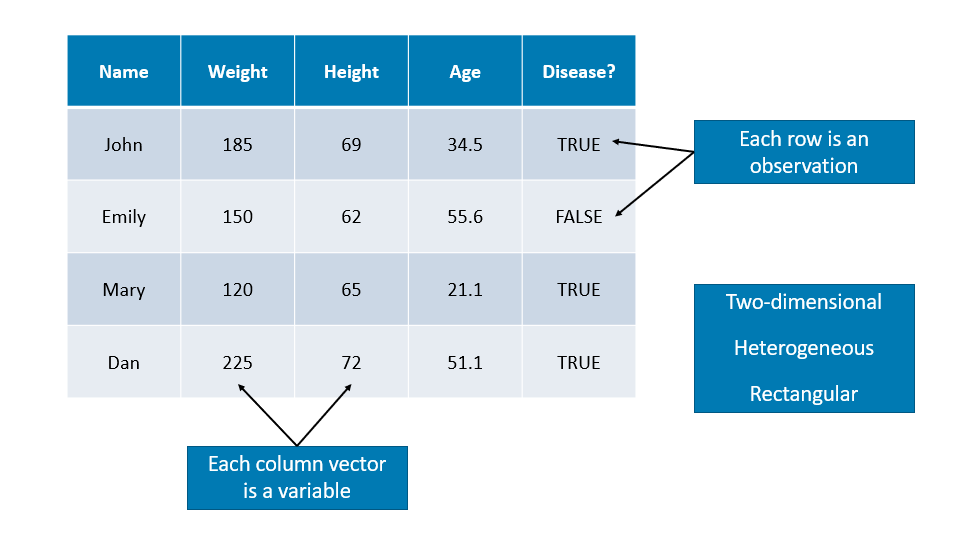
\includegraphics[width=13.56in]{png/dataframe}

Data frames combine the features of matrices and lists.

Like matrices, data frames are \textbf{rectangular}, where the columns are variables and the rows are observations of those variables. like lists, data frames can have elements (column vectors) of \textbf{different data types} (some double, some character, etc.) -- but they \textbf{must be equal length}. Real data sets usually combine variables of different types, so data frames are well suited for storage.

\begin{Shaded}
\begin{Highlighting}[]
\CommentTok{\#One way to do that}
\NormalTok{mydata }\OtherTok{\textless{}{-}} \FunctionTok{data.frame}\NormalTok{(}\AttributeTok{diabetic =} \FunctionTok{c}\NormalTok{(}\ConstantTok{TRUE}\NormalTok{, }\ConstantTok{FALSE}\NormalTok{, }\ConstantTok{TRUE}\NormalTok{, }\ConstantTok{FALSE}\NormalTok{), }
                     \AttributeTok{height =} \FunctionTok{c}\NormalTok{(}\DecValTok{65}\NormalTok{, }\DecValTok{69}\NormalTok{, }\DecValTok{71}\NormalTok{, }\DecValTok{73}\NormalTok{))}
\NormalTok{mydata}
\end{Highlighting}
\end{Shaded}

\begin{verbatim}
##   diabetic height
## 1     TRUE     65
## 2    FALSE     69
## 3     TRUE     71
## 4    FALSE     73
\end{verbatim}

\begin{Shaded}
\begin{Highlighting}[]
\FunctionTok{str}\NormalTok{(mydata)}
\end{Highlighting}
\end{Shaded}

\begin{verbatim}
## 'data.frame':    4 obs. of  2 variables:
##  $ diabetic: logi  TRUE FALSE TRUE FALSE
##  $ height  : num  65 69 71 73
\end{verbatim}

\begin{Shaded}
\begin{Highlighting}[]
\FunctionTok{dim}\NormalTok{(mydata)}
\end{Highlighting}
\end{Shaded}

\begin{verbatim}
## [1] 4 2
\end{verbatim}

\begin{Shaded}
\begin{Highlighting}[]
\CommentTok{\#Or create vectors for each column}
\NormalTok{diabetic }\OtherTok{=} \FunctionTok{c}\NormalTok{(}\ConstantTok{TRUE}\NormalTok{, }\ConstantTok{FALSE}\NormalTok{, }\ConstantTok{TRUE}\NormalTok{, }\ConstantTok{FALSE}\NormalTok{)}
\NormalTok{height }\OtherTok{=} \FunctionTok{c}\NormalTok{(}\DecValTok{65}\NormalTok{, }\DecValTok{69}\NormalTok{, }\DecValTok{71}\NormalTok{, }\DecValTok{73}\NormalTok{)}

\CommentTok{\#And include them in a data frame as follows}
\NormalTok{mydata }\OtherTok{\textless{}{-}} \FunctionTok{data.frame}\NormalTok{(diabetic, height)}
\NormalTok{mydata}
\end{Highlighting}
\end{Shaded}

\begin{verbatim}
##   diabetic height
## 1     TRUE     65
## 2    FALSE     69
## 3     TRUE     71
## 4    FALSE     73
\end{verbatim}

\begin{Shaded}
\begin{Highlighting}[]
\FunctionTok{str}\NormalTok{(mydata)}
\end{Highlighting}
\end{Shaded}

\begin{verbatim}
## 'data.frame':    4 obs. of  2 variables:
##  $ diabetic: logi  TRUE FALSE TRUE FALSE
##  $ height  : num  65 69 71 73
\end{verbatim}

\begin{Shaded}
\begin{Highlighting}[]
\FunctionTok{dim}\NormalTok{(mydata)}
\end{Highlighting}
\end{Shaded}

\begin{verbatim}
## [1] 4 2
\end{verbatim}

\begin{Shaded}
\begin{Highlighting}[]
\CommentTok{\#And more importantly, you can extend it by adding more columns}
\NormalTok{weight }\OtherTok{=} \FunctionTok{c}\NormalTok{(}\DecValTok{103}\NormalTok{, }\DecValTok{45}\NormalTok{, }\FloatTok{98.4}\NormalTok{, }\FloatTok{70.5}\NormalTok{)}
\NormalTok{mydata }\OtherTok{\textless{}{-}} \FunctionTok{data.frame}\NormalTok{(mydata, weight)}
\NormalTok{mydata}
\end{Highlighting}
\end{Shaded}

\begin{verbatim}
##   diabetic height weight
## 1     TRUE     65  103.0
## 2    FALSE     69   45.0
## 3     TRUE     71   98.4
## 4    FALSE     73   70.5
\end{verbatim}

You will have the following mistake a lot. Let's see it now so you can avoid it later.

\begin{Shaded}
\begin{Highlighting}[]
\CommentTok{\#Try running the code below separately without the comment \# and see what happens}

\CommentTok{\#mydata \textless{}{-} data.frame(diabetic = c(TRUE, FALSE, TRUE, FALSE, FALSE), }
                     \CommentTok{\#height = c(65, 69, 71, 73))}
\end{Highlighting}
\end{Shaded}

The problem in the example above is that there are a different number of rows and columns. Here are some useful tools for diagnosing this problem:

\begin{Shaded}
\begin{Highlighting}[]
\CommentTok{\#Number of columns}
\FunctionTok{ncol}\NormalTok{(mydata)}
\end{Highlighting}
\end{Shaded}

\begin{verbatim}
## [1] 3
\end{verbatim}

\begin{Shaded}
\begin{Highlighting}[]
\FunctionTok{nrow}\NormalTok{(mydata)}
\end{Highlighting}
\end{Shaded}

\begin{verbatim}
## [1] 4
\end{verbatim}

Often data you're working with has abstract column names, such as (x1, x2, x3\ldots).The \texttt{cars} is data from the 1920s on ``Speed and Stopping Distances of Cars''. There is only 2 columns shown below.

\begin{Shaded}
\begin{Highlighting}[]
\FunctionTok{colnames}\NormalTok{(datasets}\SpecialCharTok{::}\NormalTok{cars)}
\end{Highlighting}
\end{Shaded}

\begin{verbatim}
## [1] "speed" "dist"
\end{verbatim}

\begin{Shaded}
\begin{Highlighting}[]
\CommentTok{\#Using Base r:}
\FunctionTok{colnames}\NormalTok{(cars)[}\DecValTok{1}\SpecialCharTok{:}\DecValTok{2}\NormalTok{] }\OtherTok{\textless{}{-}} \FunctionTok{c}\NormalTok{(}\StringTok{"Speed (mph)"}\NormalTok{, }\StringTok{"Stopping Distance (ft)"}\NormalTok{)}
\FunctionTok{colnames}\NormalTok{(cars)}
\end{Highlighting}
\end{Shaded}

\begin{verbatim}
## [1] "Speed (mph)"            "Stopping Distance (ft)"
\end{verbatim}

\begin{Shaded}
\begin{Highlighting}[]
\CommentTok{\#Using GREP:}
\FunctionTok{colnames}\NormalTok{(cars)[}\FunctionTok{grep}\NormalTok{(}\StringTok{"dist"}\NormalTok{, }\FunctionTok{colnames}\NormalTok{(cars))] }\OtherTok{\textless{}{-}} \StringTok{"Stopping Distance (ft)"}
\FunctionTok{colnames}\NormalTok{(cars)}
\end{Highlighting}
\end{Shaded}

\begin{verbatim}
## [1] "Speed (mph)"            "Stopping Distance (ft)"
\end{verbatim}

Using \texttt{summary()} on a data frame, you get the summary statistics for each variable.

\begin{Shaded}
\begin{Highlighting}[]
\FunctionTok{summary}\NormalTok{(cars)}
\end{Highlighting}
\end{Shaded}

\begin{verbatim}
##   Speed (mph)   Stopping Distance (ft)
##  Min.   : 4.0   Min.   :  2.00        
##  1st Qu.:12.0   1st Qu.: 26.00        
##  Median :15.0   Median : 36.00        
##  Mean   :15.4   Mean   : 42.98        
##  3rd Qu.:19.0   3rd Qu.: 56.00        
##  Max.   :25.0   Max.   :120.00
\end{verbatim}

\hypertarget{subsetting-data-frames}{%
\subsection{Subsetting Data Frames}\label{subsetting-data-frames}}

Subsetting data frames can work much like subsetting matrices using square brackets, \texttt{{[},{]}}. Let's use another data given in the \texttt{ggplot2} library.

\begin{Shaded}
\begin{Highlighting}[]
\FunctionTok{library}\NormalTok{(ggplot2)}
\FunctionTok{head}\NormalTok{(mpg, }\AttributeTok{n =} \DecValTok{10}\NormalTok{)}
\end{Highlighting}
\end{Shaded}

\begin{verbatim}
## # A tibble: 10 x 11
##    manufacturer model      displ  year   cyl trans drv     cty   hwy fl    class
##    <chr>        <chr>      <dbl> <int> <int> <chr> <chr> <int> <int> <chr> <chr>
##  1 audi         a4           1.8  1999     4 auto~ f        18    29 p     comp~
##  2 audi         a4           1.8  1999     4 manu~ f        21    29 p     comp~
##  3 audi         a4           2    2008     4 manu~ f        20    31 p     comp~
##  4 audi         a4           2    2008     4 auto~ f        21    30 p     comp~
##  5 audi         a4           2.8  1999     6 auto~ f        16    26 p     comp~
##  6 audi         a4           2.8  1999     6 manu~ f        18    26 p     comp~
##  7 audi         a4           3.1  2008     6 auto~ f        18    27 p     comp~
##  8 audi         a4 quattro   1.8  1999     4 manu~ 4        18    26 p     comp~
##  9 audi         a4 quattro   1.8  1999     4 auto~ 4        16    25 p     comp~
## 10 audi         a4 quattro   2    2008     4 manu~ 4        20    28 p     comp~
\end{verbatim}

And we need to see the cars with highway mpg over 35:

\begin{Shaded}
\begin{Highlighting}[]
\NormalTok{mpg[mpg}\SpecialCharTok{$}\NormalTok{hwy }\SpecialCharTok{\textgreater{}} \DecValTok{35}\NormalTok{, }\FunctionTok{c}\NormalTok{(}\StringTok{"manufacturer"}\NormalTok{, }\StringTok{"model"}\NormalTok{, }\StringTok{"year"}\NormalTok{)]}
\end{Highlighting}
\end{Shaded}

\begin{verbatim}
## # A tibble: 6 x 3
##   manufacturer model       year
##   <chr>        <chr>      <int>
## 1 honda        civic       2008
## 2 honda        civic       2008
## 3 toyota       corolla     2008
## 4 volkswagen   jetta       1999
## 5 volkswagen   new beetle  1999
## 6 volkswagen   new beetle  1999
\end{verbatim}

An alternative would be to use the \texttt{subset()} function, which has a much more readable syntax.

\begin{Shaded}
\begin{Highlighting}[]
\FunctionTok{subset}\NormalTok{(mpg, }\AttributeTok{subset =}\NormalTok{ hwy }\SpecialCharTok{\textgreater{}} \DecValTok{35}\NormalTok{, }\AttributeTok{select =} \FunctionTok{c}\NormalTok{(}\StringTok{"manufacturer"}\NormalTok{, }\StringTok{"model"}\NormalTok{, }\StringTok{"year"}\NormalTok{))}
\end{Highlighting}
\end{Shaded}

\begin{verbatim}
## # A tibble: 6 x 3
##   manufacturer model       year
##   <chr>        <chr>      <int>
## 1 honda        civic       2008
## 2 honda        civic       2008
## 3 toyota       corolla     2008
## 4 volkswagen   jetta       1999
## 5 volkswagen   new beetle  1999
## 6 volkswagen   new beetle  1999
\end{verbatim}

Lastly, we could use the filter and select functions from the \texttt{dplyr} package which introduces the \texttt{\%\textgreater{}\%} operator from the \texttt{magrittr} package. This is not necessary for this book, however the \texttt{dplyr} package is something you should be aware of as it is becoming a popular tool in the R world.

\begin{Shaded}
\begin{Highlighting}[]
\FunctionTok{library}\NormalTok{(dplyr)}
\NormalTok{mpg }\SpecialCharTok{\%\textgreater{}\%} \FunctionTok{filter}\NormalTok{(hwy }\SpecialCharTok{\textgreater{}} \DecValTok{35}\NormalTok{) }\SpecialCharTok{\%\textgreater{}\%} \FunctionTok{select}\NormalTok{(manufacturer, model, year)}
\end{Highlighting}
\end{Shaded}

\begin{verbatim}
## # A tibble: 6 x 3
##   manufacturer model       year
##   <chr>        <chr>      <int>
## 1 honda        civic       2008
## 2 honda        civic       2008
## 3 toyota       corolla     2008
## 4 volkswagen   jetta       1999
## 5 volkswagen   new beetle  1999
## 6 volkswagen   new beetle  1999
\end{verbatim}

We will see \texttt{dplyr} later.

\hypertarget{tibble}{%
\subsection{Tibble}\label{tibble}}

Tibbles are data frames, but change some behaviors of data frames to make coding easier. To use the tibble class, you need to install the tibble package, which is part of the \texttt{tidyverse} package.

\begin{Shaded}
\begin{Highlighting}[]
\FunctionTok{library}\NormalTok{(tibble)}
\NormalTok{animal }\OtherTok{\textless{}{-}} \FunctionTok{rep}\NormalTok{(}\FunctionTok{c}\NormalTok{(}\StringTok{"sheep"}\NormalTok{, }\StringTok{"pig"}\NormalTok{), }\FunctionTok{c}\NormalTok{(}\DecValTok{3}\NormalTok{,}\DecValTok{3}\NormalTok{))}
\NormalTok{year }\OtherTok{\textless{}{-}} \FunctionTok{rep}\NormalTok{(}\DecValTok{2019}\SpecialCharTok{:}\DecValTok{2021}\NormalTok{, }\DecValTok{2}\NormalTok{)}
\NormalTok{healthy }\OtherTok{\textless{}{-}} \FunctionTok{c}\NormalTok{(}\FunctionTok{rep}\NormalTok{(}\ConstantTok{TRUE}\NormalTok{, }\DecValTok{5}\NormalTok{), }\ConstantTok{FALSE}\NormalTok{)}
\NormalTok{my\_tibble }\OtherTok{\textless{}{-}} \FunctionTok{tibble}\NormalTok{(animal, year, healthy)}
\NormalTok{my\_tibble}
\end{Highlighting}
\end{Shaded}

\begin{verbatim}
## # A tibble: 6 x 3
##   animal  year healthy
##   <chr>  <int> <lgl>  
## 1 sheep   2019 TRUE   
## 2 sheep   2020 TRUE   
## 3 sheep   2021 TRUE   
## 4 pig     2019 TRUE   
## 5 pig     2020 TRUE   
## 6 pig     2021 FALSE
\end{verbatim}

You can convert a tibble to a data frame or data frame to tibble.

\begin{Shaded}
\begin{Highlighting}[]
\NormalTok{my\_data\_frame }\OtherTok{\textless{}{-}} \FunctionTok{data.frame}\NormalTok{(animal, year,  healthy)}
\NormalTok{tt }\OtherTok{\textless{}{-}} \FunctionTok{as\_tibble}\NormalTok{(my\_data\_frame)}
\NormalTok{tt}
\end{Highlighting}
\end{Shaded}

\begin{verbatim}
## # A tibble: 6 x 3
##   animal  year healthy
##   <chr>  <int> <lgl>  
## 1 sheep   2019 TRUE   
## 2 sheep   2020 TRUE   
## 3 sheep   2021 TRUE   
## 4 pig     2019 TRUE   
## 5 pig     2020 TRUE   
## 6 pig     2021 FALSE
\end{verbatim}

\begin{Shaded}
\begin{Highlighting}[]
\CommentTok{\# Or}

\NormalTok{bck }\OtherTok{\textless{}{-}} \FunctionTok{as.data.frame}\NormalTok{(tt)}
\NormalTok{bck}
\end{Highlighting}
\end{Shaded}

\begin{verbatim}
##   animal year healthy
## 1  sheep 2019    TRUE
## 2  sheep 2020    TRUE
## 3  sheep 2021    TRUE
## 4    pig 2019    TRUE
## 5    pig 2020    TRUE
## 6    pig 2021   FALSE
\end{verbatim}

In some aspects tibbles are useful, data frames are more common.

\hypertarget{plotting-from-data-frame}{%
\subsection{Plotting from data frame}\label{plotting-from-data-frame}}

There are many good ways and packages for plotting. I'll show you one here. Visualizing the relationship between multiple variables can get messy very quickly. Here is the \texttt{ggpairs()} function in the \textbf{GGally} package \citep{Tay_2019}.

\begin{Shaded}
\begin{Highlighting}[]
\FunctionTok{library}\NormalTok{(fueleconomy)  }\CommentTok{\#install.packages("fueleconomy")}
\FunctionTok{data}\NormalTok{(vehicles)}
\NormalTok{df }\OtherTok{\textless{}{-}}\NormalTok{ vehicles[}\DecValTok{1}\SpecialCharTok{:}\DecValTok{100}\NormalTok{, ]}
\FunctionTok{str}\NormalTok{(df)}
\end{Highlighting}
\end{Shaded}

\begin{verbatim}
## tibble [100 x 12] (S3: tbl_df/tbl/data.frame)
##  $ id   : num [1:100] 13309 13310 13311 14038 14039 ...
##  $ make : chr [1:100] "Acura" "Acura" "Acura" "Acura" ...
##  $ model: chr [1:100] "2.2CL/3.0CL" "2.2CL/3.0CL" "2.2CL/3.0CL" "2.3CL/3.0CL" ...
##  $ year : num [1:100] 1997 1997 1997 1998 1998 ...
##  $ class: chr [1:100] "Subcompact Cars" "Subcompact Cars" "Subcompact Cars" "Subcompact Cars" ...
##  $ trans: chr [1:100] "Automatic 4-spd" "Manual 5-spd" "Automatic 4-spd" "Automatic 4-spd" ...
##  $ drive: chr [1:100] "Front-Wheel Drive" "Front-Wheel Drive" "Front-Wheel Drive" "Front-Wheel Drive" ...
##  $ cyl  : num [1:100] 4 4 6 4 4 6 4 4 6 5 ...
##  $ displ: num [1:100] 2.2 2.2 3 2.3 2.3 3 2.3 2.3 3 2.5 ...
##  $ fuel : chr [1:100] "Regular" "Regular" "Regular" "Regular" ...
##  $ hwy  : num [1:100] 26 28 26 27 29 26 27 29 26 23 ...
##  $ cty  : num [1:100] 20 22 18 19 21 17 20 21 17 18 ...
\end{verbatim}

Let's see how \texttt{GGally::ggpairs()} visualizes relationships between quantitative variables:

\begin{Shaded}
\begin{Highlighting}[]
\FunctionTok{library}\NormalTok{(GGally) }\CommentTok{\#install.packages("GGally")}
\NormalTok{new\_df }\OtherTok{\textless{}{-}}\NormalTok{ df[, }\FunctionTok{c}\NormalTok{(}\StringTok{"cyl"}\NormalTok{, }\StringTok{"hwy"}\NormalTok{, }\StringTok{"cty"}\NormalTok{)]}
\FunctionTok{ggpairs}\NormalTok{(new\_df)}
\end{Highlighting}
\end{Shaded}

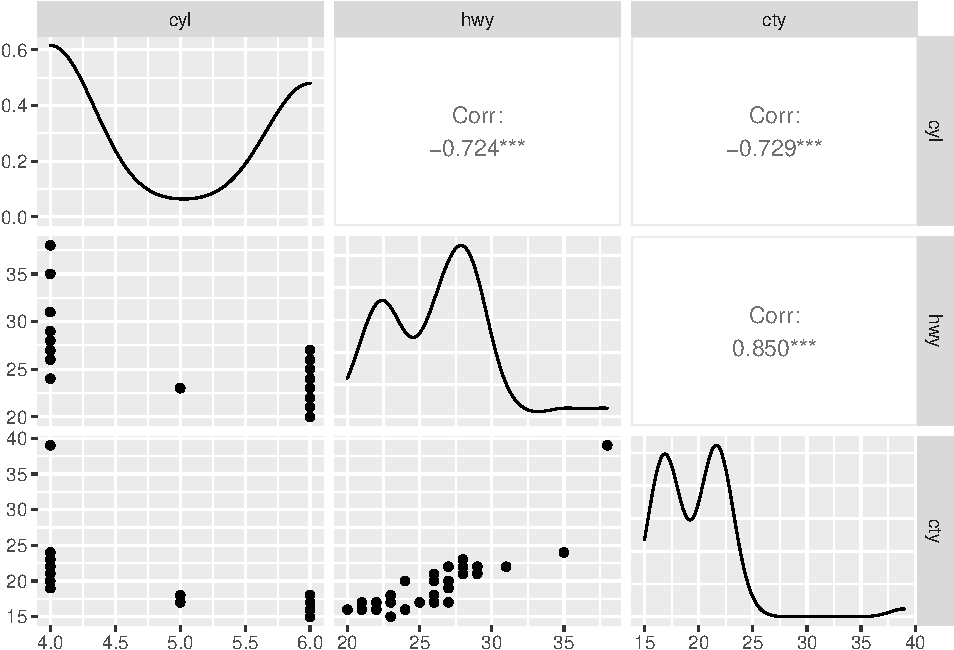
\includegraphics{02-Others_files/figure-latex/unnamed-chunk-27-1.pdf}

The visualization changes a little when we have a mix of quantitative and categorical variables. Below, fuel is a categorical variable while hwy is a quantitative variable.

\begin{Shaded}
\begin{Highlighting}[]
\NormalTok{mixed\_df }\OtherTok{\textless{}{-}}\NormalTok{ df[, }\FunctionTok{c}\NormalTok{(}\StringTok{"fuel"}\NormalTok{, }\StringTok{"hwy"}\NormalTok{)]}
\FunctionTok{ggpairs}\NormalTok{(mixed\_df)}
\end{Highlighting}
\end{Shaded}

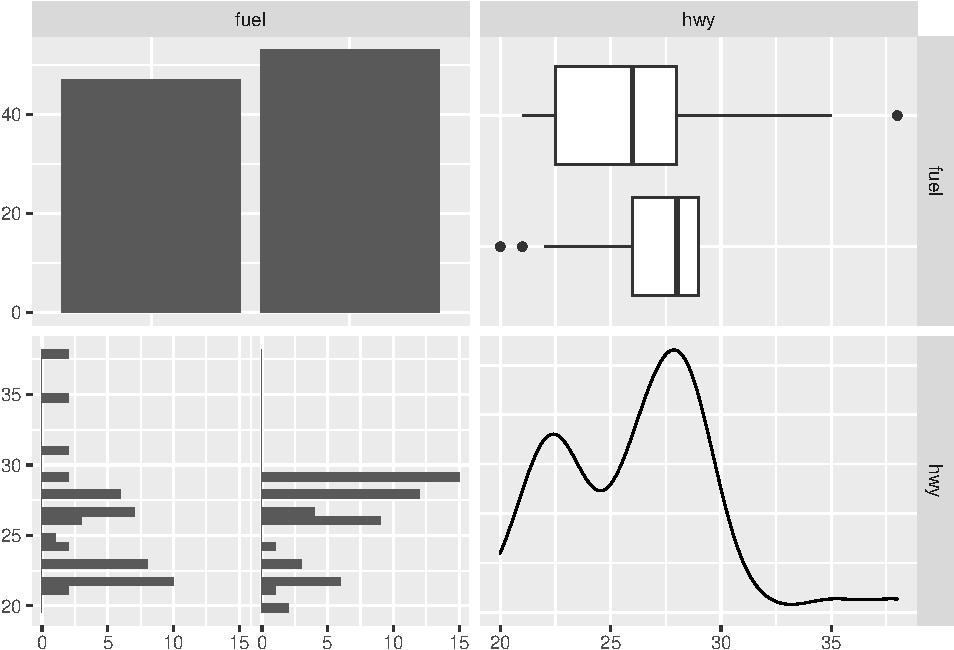
\includegraphics{02-Others_files/figure-latex/unnamed-chunk-28-1.pdf}

\hypertarget{lists}{%
\section{Lists}\label{lists}}

A list is a one-dimensional heterogeneous data structure. So it is indexed like a vector with a single integer value, but each element can contain an element of any type.

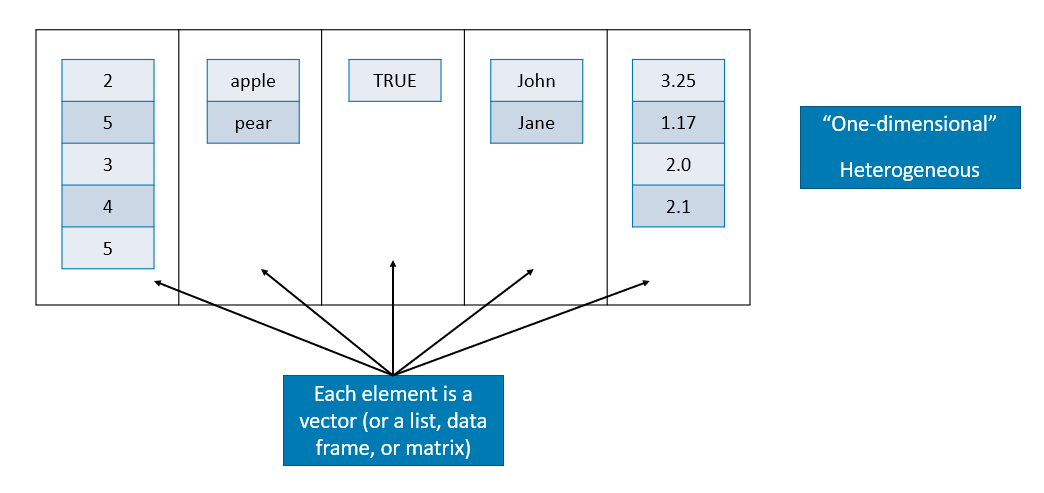
\includegraphics[width=14.5in]{png/List}

Lets look at some examples of working with them:

\begin{Shaded}
\begin{Highlighting}[]
\CommentTok{\# creation}
\NormalTok{A }\OtherTok{\textless{}{-}} \FunctionTok{list}\NormalTok{(}\DecValTok{42}\NormalTok{, }\StringTok{"Hello"}\NormalTok{, }\ConstantTok{TRUE}\NormalTok{)}
\FunctionTok{dim}\NormalTok{(A)}
\end{Highlighting}
\end{Shaded}

\begin{verbatim}
## NULL
\end{verbatim}

\begin{Shaded}
\begin{Highlighting}[]
\FunctionTok{str}\NormalTok{(A)}
\end{Highlighting}
\end{Shaded}

\begin{verbatim}
## List of 3
##  $ : num 42
##  $ : chr "Hello"
##  $ : logi TRUE
\end{verbatim}

\begin{Shaded}
\begin{Highlighting}[]
\FunctionTok{class}\NormalTok{(A)}
\end{Highlighting}
\end{Shaded}

\begin{verbatim}
## [1] "list"
\end{verbatim}

\begin{Shaded}
\begin{Highlighting}[]
\CommentTok{\# Another one}
\NormalTok{B }\OtherTok{\textless{}{-}} \FunctionTok{list}\NormalTok{(}
          \AttributeTok{a =} \FunctionTok{c}\NormalTok{(}\DecValTok{1}\NormalTok{, }\DecValTok{2}\NormalTok{, }\DecValTok{3}\NormalTok{, }\DecValTok{4}\NormalTok{),}
          \AttributeTok{b =} \ConstantTok{TRUE}\NormalTok{,}
          \AttributeTok{c =} \StringTok{"Hello!"}\NormalTok{,}
          \AttributeTok{d =} \ControlFlowTok{function}\NormalTok{(}\AttributeTok{arg =} \DecValTok{1}\NormalTok{) \{}\FunctionTok{print}\NormalTok{(}\StringTok{"Hello World!"}\NormalTok{)\},}
          \AttributeTok{X =} \FunctionTok{matrix}\NormalTok{(}\DecValTok{0}\NormalTok{, }\DecValTok{4}\NormalTok{ , }\DecValTok{4}\NormalTok{)}
\NormalTok{)}

\NormalTok{B}
\end{Highlighting}
\end{Shaded}

\begin{verbatim}
## $a
## [1] 1 2 3 4
## 
## $b
## [1] TRUE
## 
## $c
## [1] "Hello!"
## 
## $d
## function(arg = 1) {print("Hello World!")}
## 
## $X
##      [,1] [,2] [,3] [,4]
## [1,]    0    0    0    0
## [2,]    0    0    0    0
## [3,]    0    0    0    0
## [4,]    0    0    0    0
\end{verbatim}

\begin{Shaded}
\begin{Highlighting}[]
\FunctionTok{dim}\NormalTok{(B)}
\end{Highlighting}
\end{Shaded}

\begin{verbatim}
## NULL
\end{verbatim}

\begin{Shaded}
\begin{Highlighting}[]
\FunctionTok{dim}\NormalTok{(B}\SpecialCharTok{$}\NormalTok{X)}
\end{Highlighting}
\end{Shaded}

\begin{verbatim}
## [1] 4 4
\end{verbatim}

\begin{Shaded}
\begin{Highlighting}[]
\FunctionTok{str}\NormalTok{(B)}
\end{Highlighting}
\end{Shaded}

\begin{verbatim}
## List of 5
##  $ a: num [1:4] 1 2 3 4
##  $ b: logi TRUE
##  $ c: chr "Hello!"
##  $ d:function (arg = 1)  
##   ..- attr(*, "srcref")= 'srcref' int [1:8] 12 15 12 55 15 55 12 12
##   .. ..- attr(*, "srcfile")=Classes 'srcfilecopy', 'srcfile' <environment: 0x7fdd3067b200> 
##  $ X: num [1:4, 1:4] 0 0 0 0 0 0 0 0 0 0 ...
\end{verbatim}

\begin{Shaded}
\begin{Highlighting}[]
\FunctionTok{class}\NormalTok{(B)}
\end{Highlighting}
\end{Shaded}

\begin{verbatim}
## [1] "list"
\end{verbatim}

Lists can be subset using two types of syntax, the \texttt{\$} operator, and square brackets \texttt{{[}\ {]}}. The \texttt{\$} operator returns a named element of a list. The \texttt{{[}\ {]}} syntax returns a list, while the \texttt{{[}{[}\ {]}{]}} returns an element of a list.

\begin{Shaded}
\begin{Highlighting}[]
\CommentTok{\#For example to get the matrix in our list}
\NormalTok{B}\SpecialCharTok{$}\NormalTok{X}
\end{Highlighting}
\end{Shaded}

\begin{verbatim}
##      [,1] [,2] [,3] [,4]
## [1,]    0    0    0    0
## [2,]    0    0    0    0
## [3,]    0    0    0    0
## [4,]    0    0    0    0
\end{verbatim}

\begin{Shaded}
\begin{Highlighting}[]
\CommentTok{\#or}
\NormalTok{B[}\DecValTok{5}\NormalTok{]}
\end{Highlighting}
\end{Shaded}

\begin{verbatim}
## $X
##      [,1] [,2] [,3] [,4]
## [1,]    0    0    0    0
## [2,]    0    0    0    0
## [3,]    0    0    0    0
## [4,]    0    0    0    0
\end{verbatim}

\begin{Shaded}
\begin{Highlighting}[]
\CommentTok{\#or}
\NormalTok{B[[}\DecValTok{5}\NormalTok{]]}
\end{Highlighting}
\end{Shaded}

\begin{verbatim}
##      [,1] [,2] [,3] [,4]
## [1,]    0    0    0    0
## [2,]    0    0    0    0
## [3,]    0    0    0    0
## [4,]    0    0    0    0
\end{verbatim}

\begin{Shaded}
\begin{Highlighting}[]
\CommentTok{\#And to get the (1,3) element of matrix X in list B}
\NormalTok{B[[}\DecValTok{5}\NormalTok{]][}\DecValTok{1}\NormalTok{,}\DecValTok{3}\NormalTok{]}
\end{Highlighting}
\end{Shaded}

\begin{verbatim}
## [1] 0
\end{verbatim}

What's the difference between the results of \texttt{B{[}{[}5{]}{]}} and \texttt{B{[}5{]}}? The former is the third element of my\_list which is a matrix, while the latter is a list containing a single matrix element. Let's confirm this by looking at their structures.

\begin{Shaded}
\begin{Highlighting}[]
\FunctionTok{str}\NormalTok{(B[[}\DecValTok{5}\NormalTok{]])}
\end{Highlighting}
\end{Shaded}

\begin{verbatim}
##  num [1:4, 1:4] 0 0 0 0 0 0 0 0 0 0 ...
\end{verbatim}

\begin{Shaded}
\begin{Highlighting}[]
\FunctionTok{str}\NormalTok{(B[}\DecValTok{5}\NormalTok{])}
\end{Highlighting}
\end{Shaded}

\begin{verbatim}
## List of 1
##  $ X: num [1:4, 1:4] 0 0 0 0 0 0 0 0 0 0 ...
\end{verbatim}

\hypertarget{array}{%
\section{Array}\label{array}}

Array can be viewed as an extension of vector and matrix to a higher dimensional space, and still \textbf{only contains elements of the same type}.

\begin{Shaded}
\begin{Highlighting}[]
\NormalTok{A }\OtherTok{\textless{}{-}} \FunctionTok{array}\NormalTok{(}\DecValTok{1}\SpecialCharTok{:}\DecValTok{24}\NormalTok{, }\FunctionTok{c}\NormalTok{(}\DecValTok{2}\NormalTok{,}\DecValTok{3}\NormalTok{,}\DecValTok{4}\NormalTok{))}
\NormalTok{A}
\end{Highlighting}
\end{Shaded}

\begin{verbatim}
## , , 1
## 
##      [,1] [,2] [,3]
## [1,]    1    3    5
## [2,]    2    4    6
## 
## , , 2
## 
##      [,1] [,2] [,3]
## [1,]    7    9   11
## [2,]    8   10   12
## 
## , , 3
## 
##      [,1] [,2] [,3]
## [1,]   13   15   17
## [2,]   14   16   18
## 
## , , 4
## 
##      [,1] [,2] [,3]
## [1,]   19   21   23
## [2,]   20   22   24
\end{verbatim}

\begin{Shaded}
\begin{Highlighting}[]
\FunctionTok{dim}\NormalTok{(A)}
\end{Highlighting}
\end{Shaded}

\begin{verbatim}
## [1] 2 3 4
\end{verbatim}

The first argument is the data input (\texttt{1:241}). The second argument is the dimension of the array: \texttt{2} is the number of rows, \texttt{3} is the number of columns, and \texttt{4} is how many matrices we will have. Here is an example with a higher dimension:

\begin{Shaded}
\begin{Highlighting}[]
\NormalTok{y }\OtherTok{\textless{}{-}} \FunctionTok{array}\NormalTok{(}\DecValTok{0}\NormalTok{, }\FunctionTok{c}\NormalTok{(}\DecValTok{2}\NormalTok{,}\DecValTok{3}\NormalTok{,}\DecValTok{4}\NormalTok{,}\DecValTok{5}\NormalTok{))}
\NormalTok{y}
\end{Highlighting}
\end{Shaded}

\begin{verbatim}
## , , 1, 1
## 
##      [,1] [,2] [,3]
## [1,]    0    0    0
## [2,]    0    0    0
## 
## , , 2, 1
## 
##      [,1] [,2] [,3]
## [1,]    0    0    0
## [2,]    0    0    0
## 
## , , 3, 1
## 
##      [,1] [,2] [,3]
## [1,]    0    0    0
## [2,]    0    0    0
## 
## , , 4, 1
## 
##      [,1] [,2] [,3]
## [1,]    0    0    0
## [2,]    0    0    0
## 
## , , 1, 2
## 
##      [,1] [,2] [,3]
## [1,]    0    0    0
## [2,]    0    0    0
## 
## , , 2, 2
## 
##      [,1] [,2] [,3]
## [1,]    0    0    0
## [2,]    0    0    0
## 
## , , 3, 2
## 
##      [,1] [,2] [,3]
## [1,]    0    0    0
## [2,]    0    0    0
## 
## , , 4, 2
## 
##      [,1] [,2] [,3]
## [1,]    0    0    0
## [2,]    0    0    0
## 
## , , 1, 3
## 
##      [,1] [,2] [,3]
## [1,]    0    0    0
## [2,]    0    0    0
## 
## , , 2, 3
## 
##      [,1] [,2] [,3]
## [1,]    0    0    0
## [2,]    0    0    0
## 
## , , 3, 3
## 
##      [,1] [,2] [,3]
## [1,]    0    0    0
## [2,]    0    0    0
## 
## , , 4, 3
## 
##      [,1] [,2] [,3]
## [1,]    0    0    0
## [2,]    0    0    0
## 
## , , 1, 4
## 
##      [,1] [,2] [,3]
## [1,]    0    0    0
## [2,]    0    0    0
## 
## , , 2, 4
## 
##      [,1] [,2] [,3]
## [1,]    0    0    0
## [2,]    0    0    0
## 
## , , 3, 4
## 
##      [,1] [,2] [,3]
## [1,]    0    0    0
## [2,]    0    0    0
## 
## , , 4, 4
## 
##      [,1] [,2] [,3]
## [1,]    0    0    0
## [2,]    0    0    0
## 
## , , 1, 5
## 
##      [,1] [,2] [,3]
## [1,]    0    0    0
## [2,]    0    0    0
## 
## , , 2, 5
## 
##      [,1] [,2] [,3]
## [1,]    0    0    0
## [2,]    0    0    0
## 
## , , 3, 5
## 
##      [,1] [,2] [,3]
## [1,]    0    0    0
## [2,]    0    0    0
## 
## , , 4, 5
## 
##      [,1] [,2] [,3]
## [1,]    0    0    0
## [2,]    0    0    0
\end{verbatim}

\begin{Shaded}
\begin{Highlighting}[]
\FunctionTok{dim}\NormalTok{(y)}
\end{Highlighting}
\end{Shaded}

\begin{verbatim}
## [1] 2 3 4 5
\end{verbatim}

\begin{Shaded}
\begin{Highlighting}[]
\NormalTok{A[}\DecValTok{1}\NormalTok{, }\DecValTok{2}\NormalTok{, }\DecValTok{3}\NormalTok{]     }\CommentTok{\#the 3rd matrix with [1,2]}
\end{Highlighting}
\end{Shaded}

\begin{verbatim}
## [1] 15
\end{verbatim}

\begin{Shaded}
\begin{Highlighting}[]
\NormalTok{A[, , }\DecValTok{2}\NormalTok{]       }\CommentTok{\#the 2nd matrix}
\end{Highlighting}
\end{Shaded}

\begin{verbatim}
##      [,1] [,2] [,3]
## [1,]    7    9   11
## [2,]    8   10   12
\end{verbatim}

\begin{Shaded}
\begin{Highlighting}[]
\NormalTok{A[}\DecValTok{2}\NormalTok{, , }\DecValTok{4}\NormalTok{]      }\CommentTok{\#the 4th matrix, 2nd row}
\end{Highlighting}
\end{Shaded}

\begin{verbatim}
## [1] 20 22 24
\end{verbatim}

\begin{Shaded}
\begin{Highlighting}[]
\NormalTok{A[}\SpecialCharTok{{-}}\DecValTok{2}\NormalTok{, }\DecValTok{3}\NormalTok{, }\SpecialCharTok{{-}}\DecValTok{3}\NormalTok{]   }\CommentTok{\#Expect the 3rd matrix, get the 3rd columns without the 2nd rows}
\end{Highlighting}
\end{Shaded}

\begin{verbatim}
## [1]  5 11 23
\end{verbatim}

\begin{Shaded}
\begin{Highlighting}[]
\FunctionTok{apply}\NormalTok{(A, }\DecValTok{1}\NormalTok{, mean)      }\CommentTok{\#calculate the mean all rows (we have 2 rows)}
\end{Highlighting}
\end{Shaded}

\begin{verbatim}
## [1] 12 13
\end{verbatim}

\begin{Shaded}
\begin{Highlighting}[]
\CommentTok{\# Verify them}
\FunctionTok{mean}\NormalTok{(A[}\DecValTok{1}\NormalTok{, , ])         }\CommentTok{\#mean of all 1st rows}
\end{Highlighting}
\end{Shaded}

\begin{verbatim}
## [1] 12
\end{verbatim}

\begin{Shaded}
\begin{Highlighting}[]
\FunctionTok{mean}\NormalTok{(A[}\DecValTok{2}\NormalTok{, , ])         }\CommentTok{\#mean of all 2nd rows}
\end{Highlighting}
\end{Shaded}

\begin{verbatim}
## [1] 13
\end{verbatim}

\begin{Shaded}
\begin{Highlighting}[]
\FunctionTok{apply}\NormalTok{(A, }\DecValTok{2}\NormalTok{, sum)       }\CommentTok{\#calculate the sum of all columns}
\end{Highlighting}
\end{Shaded}

\begin{verbatim}
## [1]  84 100 116
\end{verbatim}

\begin{Shaded}
\begin{Highlighting}[]
\FunctionTok{apply}\NormalTok{(A, }\DecValTok{3}\NormalTok{, sd)        }\CommentTok{\#calculate the sd each matrix}
\end{Highlighting}
\end{Shaded}

\begin{verbatim}
## [1] 1.870829 1.870829 1.870829 1.870829
\end{verbatim}

\hypertarget{reading-and-writting-data-files}{%
\chapter{Reading and writting data files}\label{reading-and-writting-data-files}}

\hypertarget{reading-importing}{%
\section{Reading (importing)}\label{reading-importing}}

For any data analysis, we need data. Data come in all different formats. The data could be readable, sometimes called ascii format. Or the data could be unreadable without the original program, like an Excel workbook (.xlsx) or other statistical software formats like Stata (.dta) or SAS (.sas7bdat).

There are many ways of bringing data into your workspace. A more flexible way to import data is to use \texttt{Import\ Dataset} on the Environment tab in the upper right window of RStudio . Multiple file type options are shown, such as text, Excel, SPSS, SAS, and Stata.

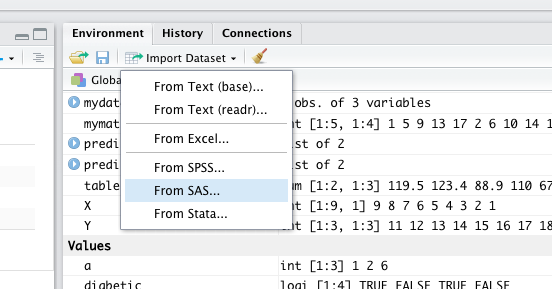
\includegraphics[width=7.67in]{png/Import}

When you read a data in other formats, they may also be imported as a data frame.

If the data is a .csv file, for example, we would also use the \texttt{read\_csv()} function from the \texttt{readr} package. Note that R has a built in function \texttt{read.csv()} that operates very similarly. The \texttt{readr} function \texttt{read\_csv()} has a number of advantages. For example, it is much faster reading larger data. It also uses the tibble package to read the data as a tibble.

\begin{Shaded}
\begin{Highlighting}[]
\FunctionTok{library}\NormalTok{(readr)}
\FunctionTok{library}\NormalTok{(RCurl)}
\NormalTok{x }\OtherTok{\textless{}{-}} \FunctionTok{getURL}\NormalTok{(}\StringTok{"https://raw.githubusercontent.com/tidyverse/readr/main/inst/extdata/mtcars.csv"}\NormalTok{)}
\NormalTok{example\_csv }\OtherTok{=} \FunctionTok{read\_csv}\NormalTok{(x, }\AttributeTok{show\_col\_types =} \ConstantTok{FALSE}\NormalTok{)}
\FunctionTok{head}\NormalTok{(example\_csv)}
\end{Highlighting}
\end{Shaded}

\begin{verbatim}
## # A tibble: 6 x 11
##     mpg   cyl  disp    hp  drat    wt  qsec    vs    am  gear  carb
##   <dbl> <dbl> <dbl> <dbl> <dbl> <dbl> <dbl> <dbl> <dbl> <dbl> <dbl>
## 1  21       6   160   110  3.9   2.62  16.5     0     1     4     4
## 2  21       6   160   110  3.9   2.88  17.0     0     1     4     4
## 3  22.8     4   108    93  3.85  2.32  18.6     1     1     4     1
## 4  21.4     6   258   110  3.08  3.22  19.4     1     0     3     1
## 5  18.7     8   360   175  3.15  3.44  17.0     0     0     3     2
## 6  18.1     6   225   105  2.76  3.46  20.2     1     0     3     1
\end{verbatim}

\begin{Shaded}
\begin{Highlighting}[]
\FunctionTok{str}\NormalTok{(example\_csv)}
\end{Highlighting}
\end{Shaded}

\begin{verbatim}
## spc_tbl_ [32 x 11] (S3: spec_tbl_df/tbl_df/tbl/data.frame)
##  $ mpg : num [1:32] 21 21 22.8 21.4 18.7 18.1 14.3 24.4 22.8 19.2 ...
##  $ cyl : num [1:32] 6 6 4 6 8 6 8 4 4 6 ...
##  $ disp: num [1:32] 160 160 108 258 360 ...
##  $ hp  : num [1:32] 110 110 93 110 175 105 245 62 95 123 ...
##  $ drat: num [1:32] 3.9 3.9 3.85 3.08 3.15 2.76 3.21 3.69 3.92 3.92 ...
##  $ wt  : num [1:32] 2.62 2.88 2.32 3.21 3.44 ...
##  $ qsec: num [1:32] 16.5 17 18.6 19.4 17 ...
##  $ vs  : num [1:32] 0 0 1 1 0 1 0 1 1 1 ...
##  $ am  : num [1:32] 1 1 1 0 0 0 0 0 0 0 ...
##  $ gear: num [1:32] 4 4 4 3 3 3 3 4 4 4 ...
##  $ carb: num [1:32] 4 4 1 1 2 1 4 2 2 4 ...
##  - attr(*, "spec")=
##   .. cols(
##   ..   mpg = col_double(),
##   ..   cyl = col_double(),
##   ..   disp = col_double(),
##   ..   hp = col_double(),
##   ..   drat = col_double(),
##   ..   wt = col_double(),
##   ..   qsec = col_double(),
##   ..   vs = col_double(),
##   ..   am = col_double(),
##   ..   gear = col_double(),
##   ..   carb = col_double()
##   .. )
##  - attr(*, "problems")=<externalptr>
\end{verbatim}

A tibble is simply a data frame that prints with sanity. Notice in the output above that we are given additional information such as dimension and variable type.

To understand more about the data set, we use the \texttt{?} operator to pull up the documentation for the data. (You can use \texttt{??} to search the Internet for more info)

\begin{Shaded}
\begin{Highlighting}[]
\NormalTok{?mtcars}
\NormalTok{??mtcars}
\CommentTok{\#View(mpg)}
\FunctionTok{head}\NormalTok{(mtcars)}
\end{Highlighting}
\end{Shaded}

\begin{verbatim}
##                    mpg cyl disp  hp drat    wt  qsec vs am gear carb
## Mazda RX4         21.0   6  160 110 3.90 2.620 16.46  0  1    4    4
## Mazda RX4 Wag     21.0   6  160 110 3.90 2.875 17.02  0  1    4    4
## Datsun 710        22.8   4  108  93 3.85 2.320 18.61  1  1    4    1
## Hornet 4 Drive    21.4   6  258 110 3.08 3.215 19.44  1  0    3    1
## Hornet Sportabout 18.7   8  360 175 3.15 3.440 17.02  0  0    3    2
## Valiant           18.1   6  225 105 2.76 3.460 20.22  1  0    3    1
\end{verbatim}

\begin{Shaded}
\begin{Highlighting}[]
\FunctionTok{tail}\NormalTok{(mtcars)}
\end{Highlighting}
\end{Shaded}

\begin{verbatim}
##                 mpg cyl  disp  hp drat    wt qsec vs am gear carb
## Porsche 914-2  26.0   4 120.3  91 4.43 2.140 16.7  0  1    5    2
## Lotus Europa   30.4   4  95.1 113 3.77 1.513 16.9  1  1    5    2
## Ford Pantera L 15.8   8 351.0 264 4.22 3.170 14.5  0  1    5    4
## Ferrari Dino   19.7   6 145.0 175 3.62 2.770 15.5  0  1    5    6
## Maserati Bora  15.0   8 301.0 335 3.54 3.570 14.6  0  1    5    8
## Volvo 142E     21.4   4 121.0 109 4.11 2.780 18.6  1  1    4    2
\end{verbatim}

After importing our data, a quick glance at the dataset can often tell us if the data were read in correctly. Use \texttt{head()} and \texttt{tail()} to look at a specified number of rows at the beginning or end of a dataset, respectively. Use \texttt{View()} on a dataset to open a spreadsheet-style view of a dataset. In RStuido, clicking on a dataset in the Environment pane will \texttt{View()} it.

\hypertarget{writing-exporting}{%
\section{Writing (exporting)}\label{writing-exporting}}

We can export our data in a number of formats, including text, Excel .xlsx, and in other statistical software formats like Stata .dta, using \texttt{write\_functions} that reverse the operations of the \texttt{read\_functions}.

Multiple objects can be stored in an R binary file (usally extension ``.Rdata'') with \texttt{save()} and then later loaded with \texttt{load()}.

I did not specify realistic path names below.

\begin{itemize}
\tightlist
\item
  Excel .csv file: \texttt{write\_csv(dat\_csv,\ file\ =\ "path/to/save/filename.csv")}
\item
  Stata .dta file: \texttt{write\_dta(dat\_csv,\ file\ =\ "path/to/save/filename.dta")}
\item
  save these objects to an .Rdata file: \texttt{save(dat\_csv,\ mydata,\ file="path/to/save/filename.Rdata")}
\end{itemize}

One last thing: if you want to save the entire workspace, \texttt{save.image()} is just a short-cut for ``save my current workspace'', i.e., \texttt{save(list\ =\ ls(all.names\ =\ TRUE),\ file\ =\ ".RData",\ envir\ =\ .GlobalEnv)}. It is also what happens with \texttt{q("yes")}.

\hypertarget{data-visualisation-with-r}{%
\chapter{Data visualisation with R}\label{data-visualisation-with-r}}

Let's first introduce the data set that will be used throughout this chapter. The data set is a part of the Ames Housing Price data, containing 165 observations and 12 features including the sale date and price.

\begin{Shaded}
\begin{Highlighting}[]
\FunctionTok{library}\NormalTok{(AmesHousing)}
\NormalTok{amesdata }\OtherTok{\textless{}{-}} \FunctionTok{make\_ames}\NormalTok{()}
\FunctionTok{str}\NormalTok{(amesdata)}
\end{Highlighting}
\end{Shaded}

\begin{verbatim}
## tibble [2,930 x 81] (S3: tbl_df/tbl/data.frame)
##  $ MS_SubClass       : Factor w/ 16 levels "One_Story_1946_and_Newer_All_Styles",..: 1 1 1 1 6 6 12 12 12 6 ...
##  $ MS_Zoning         : Factor w/ 7 levels "Floating_Village_Residential",..: 3 2 3 3 3 3 3 3 3 3 ...
##  $ Lot_Frontage      : num [1:2930] 141 80 81 93 74 78 41 43 39 60 ...
##  $ Lot_Area          : int [1:2930] 31770 11622 14267 11160 13830 9978 4920 5005 5389 7500 ...
##  $ Street            : Factor w/ 2 levels "Grvl","Pave": 2 2 2 2 2 2 2 2 2 2 ...
##  $ Alley             : Factor w/ 3 levels "Gravel","No_Alley_Access",..: 2 2 2 2 2 2 2 2 2 2 ...
##  $ Lot_Shape         : Factor w/ 4 levels "Regular","Slightly_Irregular",..: 2 1 2 1 2 2 1 2 2 1 ...
##  $ Land_Contour      : Factor w/ 4 levels "Bnk","HLS","Low",..: 4 4 4 4 4 4 4 2 4 4 ...
##  $ Utilities         : Factor w/ 3 levels "AllPub","NoSeWa",..: 1 1 1 1 1 1 1 1 1 1 ...
##  $ Lot_Config        : Factor w/ 5 levels "Corner","CulDSac",..: 1 5 1 1 5 5 5 5 5 5 ...
##  $ Land_Slope        : Factor w/ 3 levels "Gtl","Mod","Sev": 1 1 1 1 1 1 1 1 1 1 ...
##  $ Neighborhood      : Factor w/ 29 levels "North_Ames","College_Creek",..: 1 1 1 1 7 7 17 17 17 7 ...
##  $ Condition_1       : Factor w/ 9 levels "Artery","Feedr",..: 3 2 3 3 3 3 3 3 3 3 ...
##  $ Condition_2       : Factor w/ 8 levels "Artery","Feedr",..: 3 3 3 3 3 3 3 3 3 3 ...
##  $ Bldg_Type         : Factor w/ 5 levels "OneFam","TwoFmCon",..: 1 1 1 1 1 1 5 5 5 1 ...
##  $ House_Style       : Factor w/ 8 levels "One_and_Half_Fin",..: 3 3 3 3 8 8 3 3 3 8 ...
##  $ Overall_Qual      : Factor w/ 10 levels "Very_Poor","Poor",..: 6 5 6 7 5 6 8 8 8 7 ...
##  $ Overall_Cond      : Factor w/ 10 levels "Very_Poor","Poor",..: 5 6 6 5 5 6 5 5 5 5 ...
##  $ Year_Built        : int [1:2930] 1960 1961 1958 1968 1997 1998 2001 1992 1995 1999 ...
##  $ Year_Remod_Add    : int [1:2930] 1960 1961 1958 1968 1998 1998 2001 1992 1996 1999 ...
##  $ Roof_Style        : Factor w/ 6 levels "Flat","Gable",..: 4 2 4 4 2 2 2 2 2 2 ...
##  $ Roof_Matl         : Factor w/ 8 levels "ClyTile","CompShg",..: 2 2 2 2 2 2 2 2 2 2 ...
##  $ Exterior_1st      : Factor w/ 16 levels "AsbShng","AsphShn",..: 4 14 15 4 14 14 6 7 6 14 ...
##  $ Exterior_2nd      : Factor w/ 17 levels "AsbShng","AsphShn",..: 11 15 16 4 15 15 6 7 6 15 ...
##  $ Mas_Vnr_Type      : Factor w/ 5 levels "BrkCmn","BrkFace",..: 5 4 2 4 4 2 4 4 4 4 ...
##  $ Mas_Vnr_Area      : num [1:2930] 112 0 108 0 0 20 0 0 0 0 ...
##  $ Exter_Qual        : Factor w/ 4 levels "Excellent","Fair",..: 4 4 4 3 4 4 3 3 3 4 ...
##  $ Exter_Cond        : Factor w/ 5 levels "Excellent","Fair",..: 5 5 5 5 5 5 5 5 5 5 ...
##  $ Foundation        : Factor w/ 6 levels "BrkTil","CBlock",..: 2 2 2 2 3 3 3 3 3 3 ...
##  $ Bsmt_Qual         : Factor w/ 6 levels "Excellent","Fair",..: 6 6 6 6 3 6 3 3 3 6 ...
##  $ Bsmt_Cond         : Factor w/ 6 levels "Excellent","Fair",..: 3 6 6 6 6 6 6 6 6 6 ...
##  $ Bsmt_Exposure     : Factor w/ 5 levels "Av","Gd","Mn",..: 2 4 4 4 4 4 3 4 4 4 ...
##  $ BsmtFin_Type_1    : Factor w/ 7 levels "ALQ","BLQ","GLQ",..: 2 6 1 1 3 3 3 1 3 7 ...
##  $ BsmtFin_SF_1      : num [1:2930] 2 6 1 1 3 3 3 1 3 7 ...
##  $ BsmtFin_Type_2    : Factor w/ 7 levels "ALQ","BLQ","GLQ",..: 7 4 7 7 7 7 7 7 7 7 ...
##  $ BsmtFin_SF_2      : num [1:2930] 0 144 0 0 0 0 0 0 0 0 ...
##  $ Bsmt_Unf_SF       : num [1:2930] 441 270 406 1045 137 ...
##  $ Total_Bsmt_SF     : num [1:2930] 1080 882 1329 2110 928 ...
##  $ Heating           : Factor w/ 6 levels "Floor","GasA",..: 2 2 2 2 2 2 2 2 2 2 ...
##  $ Heating_QC        : Factor w/ 5 levels "Excellent","Fair",..: 2 5 5 1 3 1 1 1 1 3 ...
##  $ Central_Air       : Factor w/ 2 levels "N","Y": 2 2 2 2 2 2 2 2 2 2 ...
##  $ Electrical        : Factor w/ 6 levels "FuseA","FuseF",..: 5 5 5 5 5 5 5 5 5 5 ...
##  $ First_Flr_SF      : int [1:2930] 1656 896 1329 2110 928 926 1338 1280 1616 1028 ...
##  $ Second_Flr_SF     : int [1:2930] 0 0 0 0 701 678 0 0 0 776 ...
##  $ Low_Qual_Fin_SF   : int [1:2930] 0 0 0 0 0 0 0 0 0 0 ...
##  $ Gr_Liv_Area       : int [1:2930] 1656 896 1329 2110 1629 1604 1338 1280 1616 1804 ...
##  $ Bsmt_Full_Bath    : num [1:2930] 1 0 0 1 0 0 1 0 1 0 ...
##  $ Bsmt_Half_Bath    : num [1:2930] 0 0 0 0 0 0 0 0 0 0 ...
##  $ Full_Bath         : int [1:2930] 1 1 1 2 2 2 2 2 2 2 ...
##  $ Half_Bath         : int [1:2930] 0 0 1 1 1 1 0 0 0 1 ...
##  $ Bedroom_AbvGr     : int [1:2930] 3 2 3 3 3 3 2 2 2 3 ...
##  $ Kitchen_AbvGr     : int [1:2930] 1 1 1 1 1 1 1 1 1 1 ...
##  $ Kitchen_Qual      : Factor w/ 5 levels "Excellent","Fair",..: 5 5 3 1 5 3 3 3 3 3 ...
##  $ TotRms_AbvGrd     : int [1:2930] 7 5 6 8 6 7 6 5 5 7 ...
##  $ Functional        : Factor w/ 8 levels "Maj1","Maj2",..: 8 8 8 8 8 8 8 8 8 8 ...
##  $ Fireplaces        : int [1:2930] 2 0 0 2 1 1 0 0 1 1 ...
##  $ Fireplace_Qu      : Factor w/ 6 levels "Excellent","Fair",..: 3 4 4 6 6 3 4 4 6 6 ...
##  $ Garage_Type       : Factor w/ 7 levels "Attchd","Basment",..: 1 1 1 1 1 1 1 1 1 1 ...
##  $ Garage_Finish     : Factor w/ 4 levels "Fin","No_Garage",..: 1 4 4 1 1 1 1 3 3 1 ...
##  $ Garage_Cars       : num [1:2930] 2 1 1 2 2 2 2 2 2 2 ...
##  $ Garage_Area       : num [1:2930] 528 730 312 522 482 470 582 506 608 442 ...
##  $ Garage_Qual       : Factor w/ 6 levels "Excellent","Fair",..: 6 6 6 6 6 6 6 6 6 6 ...
##  $ Garage_Cond       : Factor w/ 6 levels "Excellent","Fair",..: 6 6 6 6 6 6 6 6 6 6 ...
##  $ Paved_Drive       : Factor w/ 3 levels "Dirt_Gravel",..: 2 3 3 3 3 3 3 3 3 3 ...
##  $ Wood_Deck_SF      : int [1:2930] 210 140 393 0 212 360 0 0 237 140 ...
##  $ Open_Porch_SF     : int [1:2930] 62 0 36 0 34 36 0 82 152 60 ...
##  $ Enclosed_Porch    : int [1:2930] 0 0 0 0 0 0 170 0 0 0 ...
##  $ Three_season_porch: int [1:2930] 0 0 0 0 0 0 0 0 0 0 ...
##  $ Screen_Porch      : int [1:2930] 0 120 0 0 0 0 0 144 0 0 ...
##  $ Pool_Area         : int [1:2930] 0 0 0 0 0 0 0 0 0 0 ...
##  $ Pool_QC           : Factor w/ 5 levels "Excellent","Fair",..: 4 4 4 4 4 4 4 4 4 4 ...
##  $ Fence             : Factor w/ 5 levels "Good_Privacy",..: 5 3 5 5 3 5 5 5 5 5 ...
##  $ Misc_Feature      : Factor w/ 6 levels "Elev","Gar2",..: 3 3 2 3 3 3 3 3 3 3 ...
##  $ Misc_Val          : int [1:2930] 0 0 12500 0 0 0 0 0 0 0 ...
##  $ Mo_Sold           : int [1:2930] 5 6 6 4 3 6 4 1 3 6 ...
##  $ Year_Sold         : int [1:2930] 2010 2010 2010 2010 2010 2010 2010 2010 2010 2010 ...
##  $ Sale_Type         : Factor w/ 10 levels "COD","Con","ConLD",..: 10 10 10 10 10 10 10 10 10 10 ...
##  $ Sale_Condition    : Factor w/ 6 levels "Abnorml","AdjLand",..: 5 5 5 5 5 5 5 5 5 5 ...
##  $ Sale_Price        : int [1:2930] 215000 105000 172000 244000 189900 195500 213500 191500 236500 189000 ...
##  $ Longitude         : num [1:2930] -93.6 -93.6 -93.6 -93.6 -93.6 ...
##  $ Latitude          : num [1:2930] 42.1 42.1 42.1 42.1 42.1 ...
##  - attr(*, "spec")=List of 2
##   ..$ cols   :List of 82
##   .. ..$ Order          : list()
##   .. .. ..- attr(*, "class")= chr [1:2] "collector_integer" "collector"
##   .. ..$ PID            : list()
##   .. .. ..- attr(*, "class")= chr [1:2] "collector_character" "collector"
##   .. ..$ MS SubClass    : list()
##   .. .. ..- attr(*, "class")= chr [1:2] "collector_character" "collector"
##   .. ..$ MS Zoning      : list()
##   .. .. ..- attr(*, "class")= chr [1:2] "collector_character" "collector"
##   .. ..$ Lot Frontage   : list()
##   .. .. ..- attr(*, "class")= chr [1:2] "collector_integer" "collector"
##   .. ..$ Lot Area       : list()
##   .. .. ..- attr(*, "class")= chr [1:2] "collector_integer" "collector"
##   .. ..$ Street         : list()
##   .. .. ..- attr(*, "class")= chr [1:2] "collector_character" "collector"
##   .. ..$ Alley          : list()
##   .. .. ..- attr(*, "class")= chr [1:2] "collector_character" "collector"
##   .. ..$ Lot Shape      : list()
##   .. .. ..- attr(*, "class")= chr [1:2] "collector_character" "collector"
##   .. ..$ Land Contour   : list()
##   .. .. ..- attr(*, "class")= chr [1:2] "collector_character" "collector"
##   .. ..$ Utilities      : list()
##   .. .. ..- attr(*, "class")= chr [1:2] "collector_character" "collector"
##   .. ..$ Lot Config     : list()
##   .. .. ..- attr(*, "class")= chr [1:2] "collector_character" "collector"
##   .. ..$ Land Slope     : list()
##   .. .. ..- attr(*, "class")= chr [1:2] "collector_character" "collector"
##   .. ..$ Neighborhood   : list()
##   .. .. ..- attr(*, "class")= chr [1:2] "collector_character" "collector"
##   .. ..$ Condition 1    : list()
##   .. .. ..- attr(*, "class")= chr [1:2] "collector_character" "collector"
##   .. ..$ Condition 2    : list()
##   .. .. ..- attr(*, "class")= chr [1:2] "collector_character" "collector"
##   .. ..$ Bldg Type      : list()
##   .. .. ..- attr(*, "class")= chr [1:2] "collector_character" "collector"
##   .. ..$ House Style    : list()
##   .. .. ..- attr(*, "class")= chr [1:2] "collector_character" "collector"
##   .. ..$ Overall Qual   : list()
##   .. .. ..- attr(*, "class")= chr [1:2] "collector_integer" "collector"
##   .. ..$ Overall Cond   : list()
##   .. .. ..- attr(*, "class")= chr [1:2] "collector_integer" "collector"
##   .. ..$ Year Built     : list()
##   .. .. ..- attr(*, "class")= chr [1:2] "collector_integer" "collector"
##   .. ..$ Year Remod/Add : list()
##   .. .. ..- attr(*, "class")= chr [1:2] "collector_integer" "collector"
##   .. ..$ Roof Style     : list()
##   .. .. ..- attr(*, "class")= chr [1:2] "collector_character" "collector"
##   .. ..$ Roof Matl      : list()
##   .. .. ..- attr(*, "class")= chr [1:2] "collector_character" "collector"
##   .. ..$ Exterior 1st   : list()
##   .. .. ..- attr(*, "class")= chr [1:2] "collector_character" "collector"
##   .. ..$ Exterior 2nd   : list()
##   .. .. ..- attr(*, "class")= chr [1:2] "collector_character" "collector"
##   .. ..$ Mas Vnr Type   : list()
##   .. .. ..- attr(*, "class")= chr [1:2] "collector_character" "collector"
##   .. ..$ Mas Vnr Area   : list()
##   .. .. ..- attr(*, "class")= chr [1:2] "collector_integer" "collector"
##   .. ..$ Exter Qual     : list()
##   .. .. ..- attr(*, "class")= chr [1:2] "collector_character" "collector"
##   .. ..$ Exter Cond     : list()
##   .. .. ..- attr(*, "class")= chr [1:2] "collector_character" "collector"
##   .. ..$ Foundation     : list()
##   .. .. ..- attr(*, "class")= chr [1:2] "collector_character" "collector"
##   .. ..$ Bsmt Qual      : list()
##   .. .. ..- attr(*, "class")= chr [1:2] "collector_character" "collector"
##   .. ..$ Bsmt Cond      : list()
##   .. .. ..- attr(*, "class")= chr [1:2] "collector_character" "collector"
##   .. ..$ Bsmt Exposure  : list()
##   .. .. ..- attr(*, "class")= chr [1:2] "collector_character" "collector"
##   .. ..$ BsmtFin Type 1 : list()
##   .. .. ..- attr(*, "class")= chr [1:2] "collector_character" "collector"
##   .. ..$ BsmtFin SF 1   : list()
##   .. .. ..- attr(*, "class")= chr [1:2] "collector_integer" "collector"
##   .. ..$ BsmtFin Type 2 : list()
##   .. .. ..- attr(*, "class")= chr [1:2] "collector_character" "collector"
##   .. ..$ BsmtFin SF 2   : list()
##   .. .. ..- attr(*, "class")= chr [1:2] "collector_integer" "collector"
##   .. ..$ Bsmt Unf SF    : list()
##   .. .. ..- attr(*, "class")= chr [1:2] "collector_integer" "collector"
##   .. ..$ Total Bsmt SF  : list()
##   .. .. ..- attr(*, "class")= chr [1:2] "collector_integer" "collector"
##   .. ..$ Heating        : list()
##   .. .. ..- attr(*, "class")= chr [1:2] "collector_character" "collector"
##   .. ..$ Heating QC     : list()
##   .. .. ..- attr(*, "class")= chr [1:2] "collector_character" "collector"
##   .. ..$ Central Air    : list()
##   .. .. ..- attr(*, "class")= chr [1:2] "collector_character" "collector"
##   .. ..$ Electrical     : list()
##   .. .. ..- attr(*, "class")= chr [1:2] "collector_character" "collector"
##   .. ..$ 1st Flr SF     : list()
##   .. .. ..- attr(*, "class")= chr [1:2] "collector_integer" "collector"
##   .. ..$ 2nd Flr SF     : list()
##   .. .. ..- attr(*, "class")= chr [1:2] "collector_integer" "collector"
##   .. ..$ Low Qual Fin SF: list()
##   .. .. ..- attr(*, "class")= chr [1:2] "collector_integer" "collector"
##   .. ..$ Gr Liv Area    : list()
##   .. .. ..- attr(*, "class")= chr [1:2] "collector_integer" "collector"
##   .. ..$ Bsmt Full Bath : list()
##   .. .. ..- attr(*, "class")= chr [1:2] "collector_integer" "collector"
##   .. ..$ Bsmt Half Bath : list()
##   .. .. ..- attr(*, "class")= chr [1:2] "collector_integer" "collector"
##   .. ..$ Full Bath      : list()
##   .. .. ..- attr(*, "class")= chr [1:2] "collector_integer" "collector"
##   .. ..$ Half Bath      : list()
##   .. .. ..- attr(*, "class")= chr [1:2] "collector_integer" "collector"
##   .. ..$ Bedroom AbvGr  : list()
##   .. .. ..- attr(*, "class")= chr [1:2] "collector_integer" "collector"
##   .. ..$ Kitchen AbvGr  : list()
##   .. .. ..- attr(*, "class")= chr [1:2] "collector_integer" "collector"
##   .. ..$ Kitchen Qual   : list()
##   .. .. ..- attr(*, "class")= chr [1:2] "collector_character" "collector"
##   .. ..$ TotRms AbvGrd  : list()
##   .. .. ..- attr(*, "class")= chr [1:2] "collector_integer" "collector"
##   .. ..$ Functional     : list()
##   .. .. ..- attr(*, "class")= chr [1:2] "collector_character" "collector"
##   .. ..$ Fireplaces     : list()
##   .. .. ..- attr(*, "class")= chr [1:2] "collector_integer" "collector"
##   .. ..$ Fireplace Qu   : list()
##   .. .. ..- attr(*, "class")= chr [1:2] "collector_character" "collector"
##   .. ..$ Garage Type    : list()
##   .. .. ..- attr(*, "class")= chr [1:2] "collector_character" "collector"
##   .. ..$ Garage Yr Blt  : list()
##   .. .. ..- attr(*, "class")= chr [1:2] "collector_integer" "collector"
##   .. ..$ Garage Finish  : list()
##   .. .. ..- attr(*, "class")= chr [1:2] "collector_character" "collector"
##   .. ..$ Garage Cars    : list()
##   .. .. ..- attr(*, "class")= chr [1:2] "collector_integer" "collector"
##   .. ..$ Garage Area    : list()
##   .. .. ..- attr(*, "class")= chr [1:2] "collector_integer" "collector"
##   .. ..$ Garage Qual    : list()
##   .. .. ..- attr(*, "class")= chr [1:2] "collector_character" "collector"
##   .. ..$ Garage Cond    : list()
##   .. .. ..- attr(*, "class")= chr [1:2] "collector_character" "collector"
##   .. ..$ Paved Drive    : list()
##   .. .. ..- attr(*, "class")= chr [1:2] "collector_character" "collector"
##   .. ..$ Wood Deck SF   : list()
##   .. .. ..- attr(*, "class")= chr [1:2] "collector_integer" "collector"
##   .. ..$ Open Porch SF  : list()
##   .. .. ..- attr(*, "class")= chr [1:2] "collector_integer" "collector"
##   .. ..$ Enclosed Porch : list()
##   .. .. ..- attr(*, "class")= chr [1:2] "collector_integer" "collector"
##   .. ..$ 3Ssn Porch     : list()
##   .. .. ..- attr(*, "class")= chr [1:2] "collector_integer" "collector"
##   .. ..$ Screen Porch   : list()
##   .. .. ..- attr(*, "class")= chr [1:2] "collector_integer" "collector"
##   .. ..$ Pool Area      : list()
##   .. .. ..- attr(*, "class")= chr [1:2] "collector_integer" "collector"
##   .. ..$ Pool QC        : list()
##   .. .. ..- attr(*, "class")= chr [1:2] "collector_character" "collector"
##   .. ..$ Fence          : list()
##   .. .. ..- attr(*, "class")= chr [1:2] "collector_character" "collector"
##   .. ..$ Misc Feature   : list()
##   .. .. ..- attr(*, "class")= chr [1:2] "collector_character" "collector"
##   .. ..$ Misc Val       : list()
##   .. .. ..- attr(*, "class")= chr [1:2] "collector_integer" "collector"
##   .. ..$ Mo Sold        : list()
##   .. .. ..- attr(*, "class")= chr [1:2] "collector_integer" "collector"
##   .. ..$ Yr Sold        : list()
##   .. .. ..- attr(*, "class")= chr [1:2] "collector_integer" "collector"
##   .. ..$ Sale Type      : list()
##   .. .. ..- attr(*, "class")= chr [1:2] "collector_character" "collector"
##   .. ..$ Sale Condition : list()
##   .. .. ..- attr(*, "class")= chr [1:2] "collector_character" "collector"
##   .. ..$ SalePrice      : list()
##   .. .. ..- attr(*, "class")= chr [1:2] "collector_integer" "collector"
##   ..$ default: list()
##   .. ..- attr(*, "class")= chr [1:2] "collector_guess" "collector"
##   ..- attr(*, "class")= chr "col_spec"
\end{verbatim}

\hypertarget{scatterplots}{%
\section{Scatterplots}\label{scatterplots}}

Are the bigger houses more expensive? In base R, we can use the \texttt{plot()} function to generate this scatterplot with the first argument being the variable on the x-axis and the second argument being the variable on the y-axis.

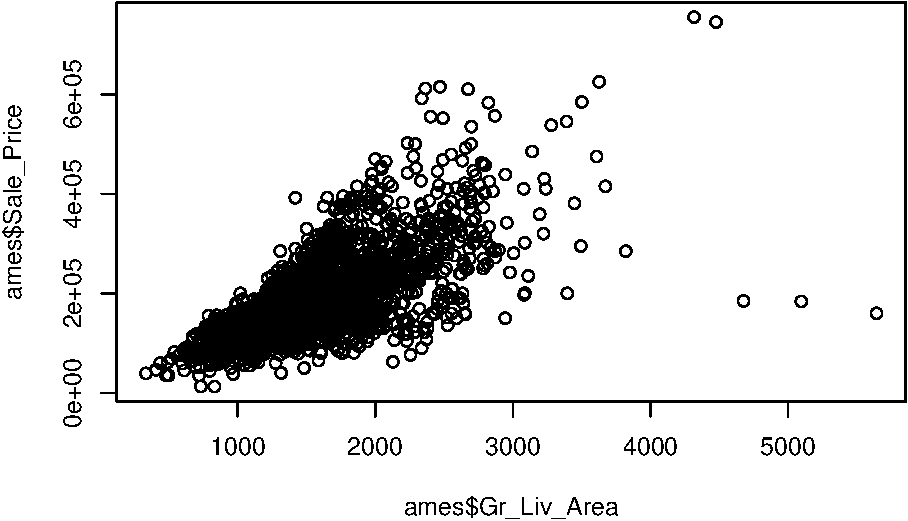
\includegraphics{04-visual_files/figure-latex/pressure-1.pdf}

It's OK but not nice. The \texttt{plot()} function provides a rich capability of customization by setting the graphical parameters.

\begin{Shaded}
\begin{Highlighting}[]
\FunctionTok{plot}\NormalTok{(amesdata}\SpecialCharTok{$}\NormalTok{Gr\_Liv\_Area, amesdata}\SpecialCharTok{$}\NormalTok{Sale\_Price, }
     \AttributeTok{col =} \StringTok{"red"}\NormalTok{, }
     \AttributeTok{xlab =} \StringTok{"Living Area"}\NormalTok{, }
     \AttributeTok{ylab =} \StringTok{"Sale Price"}\NormalTok{, }
     \AttributeTok{main =} \StringTok{"Sale Price vs. Living Area"}\NormalTok{,  }
     \AttributeTok{pch =} \DecValTok{1}\NormalTok{, }\CommentTok{\#Shape of the points}
     \AttributeTok{cex =} \DecValTok{1}\NormalTok{) }\CommentTok{\#Size of text and symbols}
\end{Highlighting}
\end{Shaded}

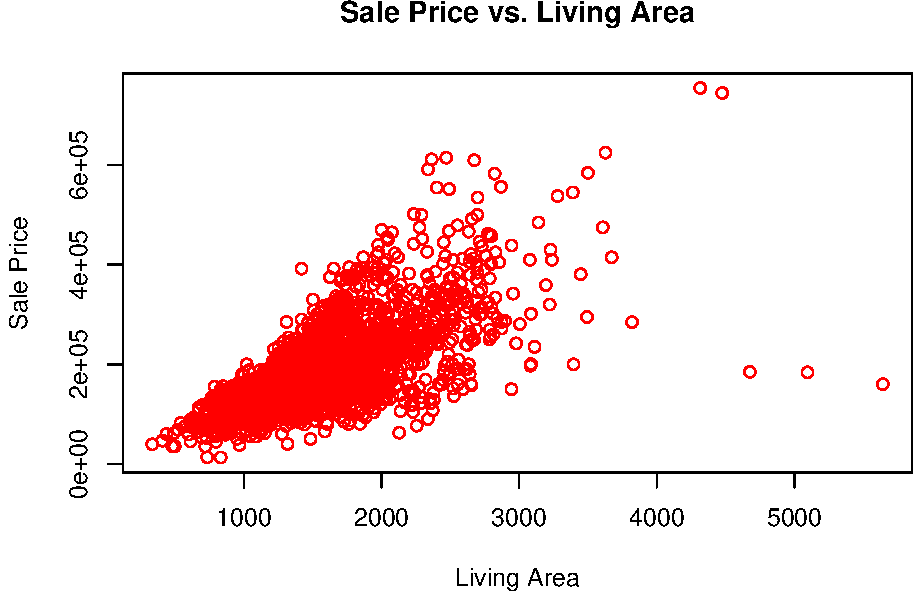
\includegraphics{04-visual_files/figure-latex/unnamed-chunk-2-1.pdf}

Although the \texttt{plot()} function gets the work done, the \texttt{ggplot2} package provides a superior user experience. It's a member of the \texttt{tidyverse} package, you don't need to install it separately if tidyverse was already installed.

\begin{Shaded}
\begin{Highlighting}[]
\FunctionTok{library}\NormalTok{(ggplot2)}
\FunctionTok{ggplot}\NormalTok{(}\AttributeTok{data =}\NormalTok{ amesdata) }\SpecialCharTok{+} 
  \FunctionTok{geom\_point}\NormalTok{(}\AttributeTok{mapping =} \FunctionTok{aes}\NormalTok{(}\AttributeTok{x =}\NormalTok{ Gr\_Liv\_Area, }\AttributeTok{y =}\NormalTok{ Sale\_Price))}
\end{Highlighting}
\end{Shaded}

\includegraphics{04-visual_files/figure-latex/unnamed-chunk-3-1.pdf}

In a nutshell, \texttt{ggplot2} implements the grammar of graphics, a coherent system for describing and building graphs. We always start with the function \texttt{ggplot()} with a data frame or tibble as its argument. To generate a scatterplot, you can add a layer using the \texttt{+} operator followed by the \texttt{geom\_point()} function, which is one of the many available geoms in ggplot. Inside \texttt{geom\_point()}, you need to set the value of the mapping argument. The mapping argument takes a functional form as \texttt{mapping\ =\ aes()}, where the \texttt{aes} is short for aesthetics. For example, you can use \texttt{aes()} to tell ggplot to use which variable on the x-axis, which variable on the y-axis.

\begin{Shaded}
\begin{Highlighting}[]
\FunctionTok{ggplot}\NormalTok{(}\AttributeTok{data =}\NormalTok{ amesdata) }\SpecialCharTok{+} 
  \FunctionTok{geom\_point}\NormalTok{(}\AttributeTok{mapping =} \FunctionTok{aes}\NormalTok{(Gr\_Liv\_Area, }\AttributeTok{y =}\NormalTok{ Sale\_Price), }
             \AttributeTok{color =} \StringTok{"red"}\NormalTok{,}
             \AttributeTok{shape =} \DecValTok{2}\NormalTok{,}
             \AttributeTok{size =} \FloatTok{0.5}\NormalTok{,}
             \AttributeTok{alpha =} \FloatTok{0.3}\NormalTok{) }\CommentTok{\#transparency level of the points}
\end{Highlighting}
\end{Shaded}

\includegraphics{04-visual_files/figure-latex/unnamed-chunk-4-1.pdf}

Suppose we want to use different colors according to the different \texttt{House\_Style} in the scatterplot.

\begin{Shaded}
\begin{Highlighting}[]
\FunctionTok{ggplot}\NormalTok{(}\AttributeTok{data =}\NormalTok{ amesdata) }\SpecialCharTok{+} 
  \FunctionTok{geom\_point}\NormalTok{(}\AttributeTok{mapping =} \FunctionTok{aes}\NormalTok{(}\AttributeTok{x =}\NormalTok{ Gr\_Liv\_Area, }
                           \AttributeTok{y =}\NormalTok{ Sale\_Price, }
                           \AttributeTok{color =}\NormalTok{ House\_Style), }
             \AttributeTok{size =} \DecValTok{1}\NormalTok{)}
\end{Highlighting}
\end{Shaded}

\includegraphics{04-visual_files/figure-latex/unnamed-chunk-5-1.pdf}

In addition to color, you can also map a discrete variable to the size aesthetic.

\begin{Shaded}
\begin{Highlighting}[]
\FunctionTok{ggplot}\NormalTok{(}\AttributeTok{data =}\NormalTok{ amesdata) }\SpecialCharTok{+} 
  \FunctionTok{geom\_point}\NormalTok{(}\AttributeTok{mapping =} \FunctionTok{aes}\NormalTok{(}\AttributeTok{x =}\NormalTok{ Gr\_Liv\_Area, }
                           \AttributeTok{y =}\NormalTok{ Sale\_Price, }
                           \AttributeTok{size =}\NormalTok{ House\_Style), }
             \AttributeTok{alpha =} \FloatTok{0.5}\NormalTok{)}
\end{Highlighting}
\end{Shaded}

\includegraphics{04-visual_files/figure-latex/unnamed-chunk-6-1.pdf}

Or

\begin{Shaded}
\begin{Highlighting}[]
\FunctionTok{ggplot}\NormalTok{(}\AttributeTok{data =}\NormalTok{ amesdata) }\SpecialCharTok{+} 
  \FunctionTok{geom\_point}\NormalTok{(}\AttributeTok{mapping =} \FunctionTok{aes}\NormalTok{(}\AttributeTok{x =}\NormalTok{ Gr\_Liv\_Area, }
                           \AttributeTok{y =}\NormalTok{ Sale\_Price, }
                           \AttributeTok{shape =}\NormalTok{ Exter\_Qual), }
             \AttributeTok{alpha =} \FloatTok{0.5}\NormalTok{,}
             \AttributeTok{size =} \DecValTok{2}\NormalTok{)}
\end{Highlighting}
\end{Shaded}

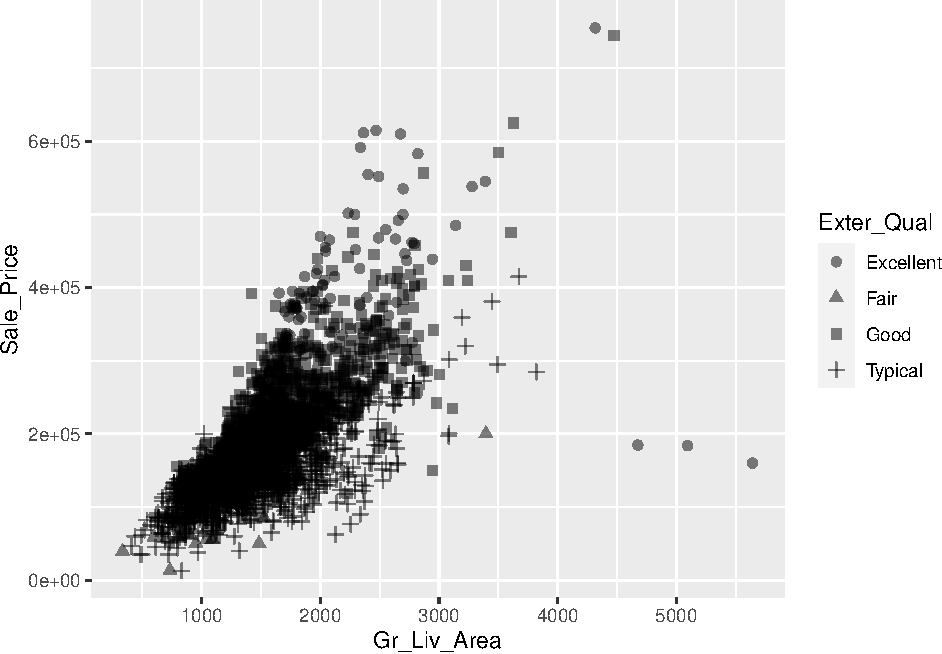
\includegraphics{04-visual_files/figure-latex/unnamed-chunk-7-1.pdf}

and multiple mapping:

\begin{Shaded}
\begin{Highlighting}[]
\FunctionTok{ggplot}\NormalTok{(}\AttributeTok{data =}\NormalTok{ amesdata) }\SpecialCharTok{+} 
  \FunctionTok{geom\_point}\NormalTok{(}\AttributeTok{mapping =} \FunctionTok{aes}\NormalTok{(}\AttributeTok{x =}\NormalTok{ Gr\_Liv\_Area, }
                           \AttributeTok{y =}\NormalTok{ Sale\_Price, }
                           \AttributeTok{shape =}\NormalTok{ Exter\_Qual,}
                           \AttributeTok{color =}\NormalTok{ Central\_Air), }
             \AttributeTok{alpha =} \FloatTok{0.5}\NormalTok{,}
             \AttributeTok{size =} \DecValTok{2}\NormalTok{)}
\end{Highlighting}
\end{Shaded}

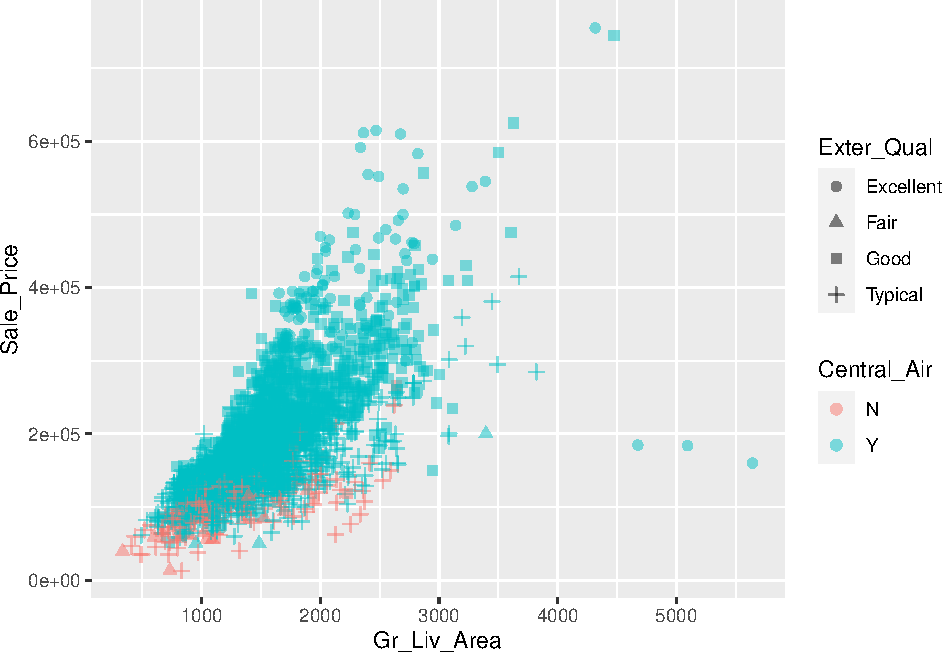
\includegraphics{04-visual_files/figure-latex/unnamed-chunk-8-1.pdf}

\hypertarget{smootlines}{%
\section{Smootlines}\label{smootlines}}

\begin{Shaded}
\begin{Highlighting}[]
\FunctionTok{ggplot}\NormalTok{(}\AttributeTok{data =}\NormalTok{ amesdata) }\SpecialCharTok{+} 
  \FunctionTok{geom\_smooth}\NormalTok{(}\AttributeTok{mapping =} \FunctionTok{aes}\NormalTok{(}\AttributeTok{x =}\NormalTok{ Gr\_Liv\_Area, }
                           \AttributeTok{y =}\NormalTok{ Sale\_Price), }
              \AttributeTok{size =} \FloatTok{1.5}\NormalTok{)}
\end{Highlighting}
\end{Shaded}

\begin{verbatim}
## `geom_smooth()` using method = 'gam' and formula 'y ~ s(x, bs = "cs")'
\end{verbatim}

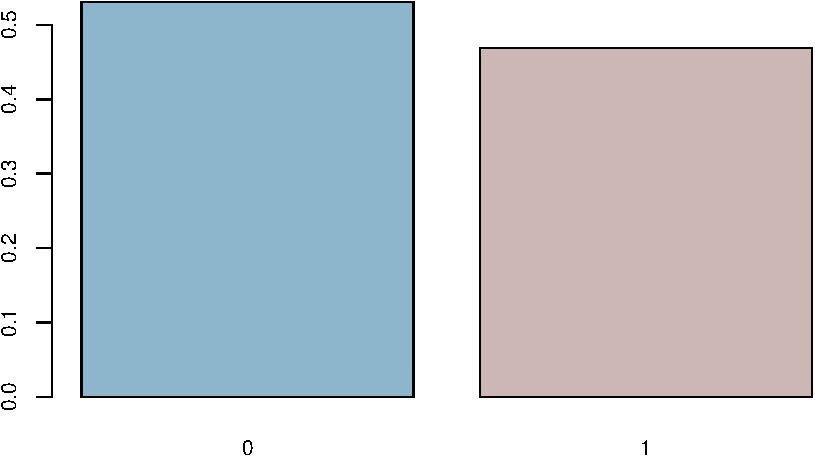
\includegraphics{04-visual_files/figure-latex/unnamed-chunk-9-1.pdf}

\begin{Shaded}
\begin{Highlighting}[]
\FunctionTok{ggplot}\NormalTok{(}\AttributeTok{data =}\NormalTok{ amesdata) }\SpecialCharTok{+} 
  \FunctionTok{geom\_smooth}\NormalTok{(}\AttributeTok{mapping =} \FunctionTok{aes}\NormalTok{(}\AttributeTok{x =}\NormalTok{ Gr\_Liv\_Area, }
                           \AttributeTok{y =}\NormalTok{ Sale\_Price), }
              \AttributeTok{size =} \FloatTok{1.5}\NormalTok{,}
              \AttributeTok{method =} \StringTok{"lm"}\NormalTok{)}
\end{Highlighting}
\end{Shaded}

\begin{verbatim}
## `geom_smooth()` using formula 'y ~ x'
\end{verbatim}

\includegraphics{04-visual_files/figure-latex/unnamed-chunk-10-1.pdf}

And

\begin{Shaded}
\begin{Highlighting}[]
\FunctionTok{ggplot}\NormalTok{(}\AttributeTok{data =}\NormalTok{ amesdata) }\SpecialCharTok{+} 
  \FunctionTok{geom\_point}\NormalTok{(}\AttributeTok{mapping =} \FunctionTok{aes}\NormalTok{(}\AttributeTok{x =}\NormalTok{ Gr\_Liv\_Area, }
                           \AttributeTok{y =}\NormalTok{ Sale\_Price)) }\SpecialCharTok{+}
  \FunctionTok{geom\_smooth}\NormalTok{(}\AttributeTok{mapping =} \FunctionTok{aes}\NormalTok{(}\AttributeTok{x =}\NormalTok{ Gr\_Liv\_Area, }
                           \AttributeTok{y =}\NormalTok{ Sale\_Price)) }
\end{Highlighting}
\end{Shaded}

\begin{verbatim}
## `geom_smooth()` using method = 'gam' and formula 'y ~ s(x, bs = "cs")'
\end{verbatim}

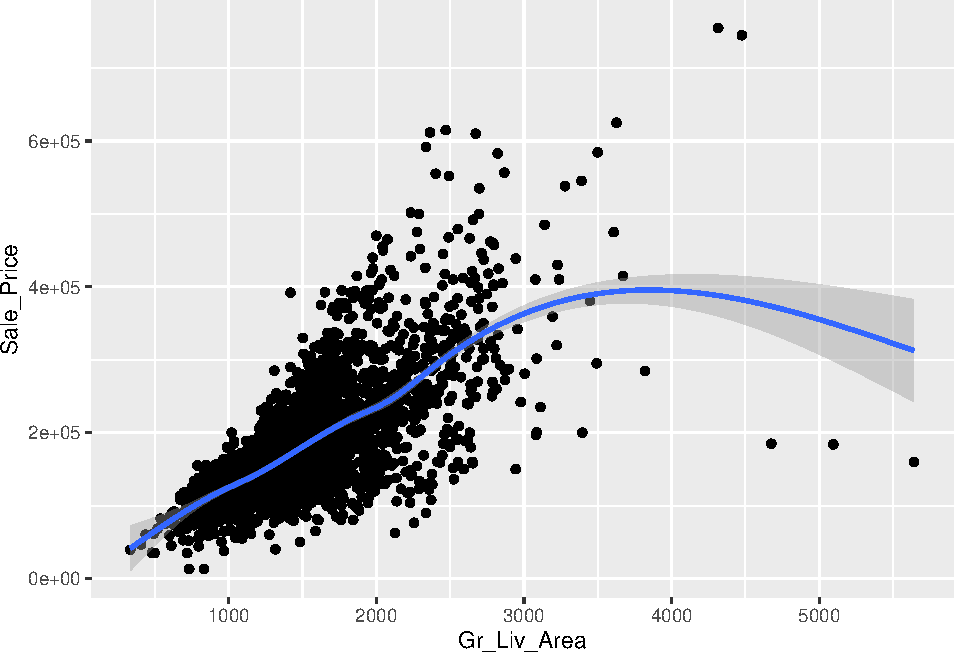
\includegraphics{04-visual_files/figure-latex/unnamed-chunk-11-1.pdf}

\begin{Shaded}
\begin{Highlighting}[]
\CommentTok{\# Or with global mapping}

\FunctionTok{ggplot}\NormalTok{(}\AttributeTok{data =}\NormalTok{ amesdata, }
       \AttributeTok{mapping =} \FunctionTok{aes}\NormalTok{(}\AttributeTok{x =}\NormalTok{ Gr\_Liv\_Area, }
                     \AttributeTok{y =}\NormalTok{ Sale\_Price,}
                     \AttributeTok{color =}\NormalTok{ Central\_Air)) }\SpecialCharTok{+}
  \FunctionTok{geom\_point}\NormalTok{() }\SpecialCharTok{+}
  \FunctionTok{geom\_smooth}\NormalTok{() }
\end{Highlighting}
\end{Shaded}

\begin{verbatim}
## `geom_smooth()` using method = 'gam' and formula 'y ~ s(x, bs = "cs")'
\end{verbatim}

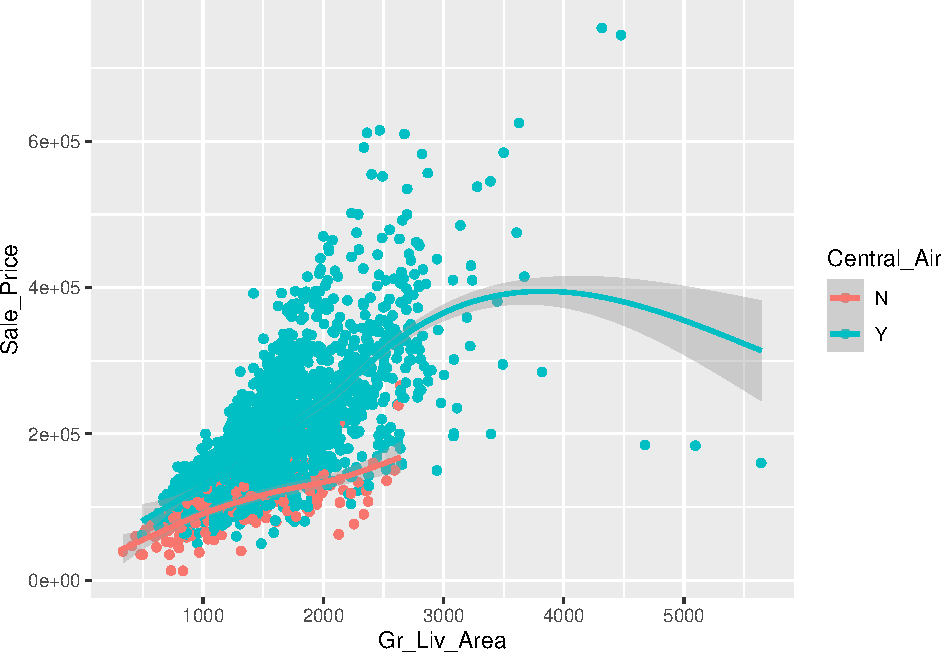
\includegraphics{04-visual_files/figure-latex/unnamed-chunk-11-2.pdf}

\hypertarget{histograms-density}{%
\section{Histograms \& Density}\label{histograms-density}}

How do we visualize continuous variables? One popular plot is called histograms.

\begin{Shaded}
\begin{Highlighting}[]
\FunctionTok{hist}\NormalTok{(amesdata}\SpecialCharTok{$}\NormalTok{Sale\_Price)}
\end{Highlighting}
\end{Shaded}

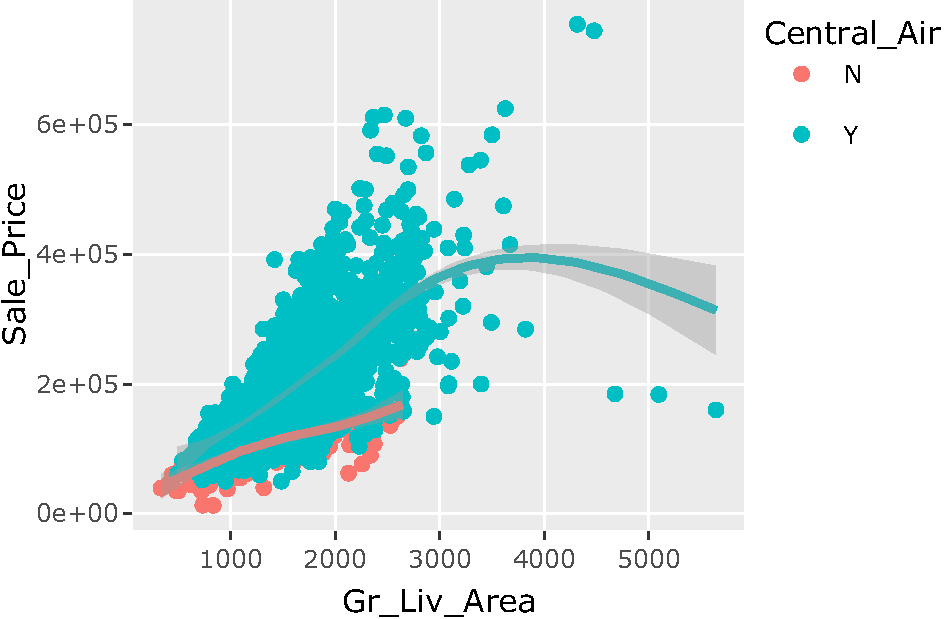
\includegraphics{04-visual_files/figure-latex/unnamed-chunk-12-1.pdf}

And density with ggplot

\begin{Shaded}
\begin{Highlighting}[]
\FunctionTok{ggplot}\NormalTok{(}\AttributeTok{data =}\NormalTok{ amesdata, }\FunctionTok{aes}\NormalTok{(}\AttributeTok{x =}\NormalTok{ Sale\_Price)) }\SpecialCharTok{+}
  \FunctionTok{geom\_histogram}\NormalTok{(}\FunctionTok{aes}\NormalTok{(}\AttributeTok{y =}\NormalTok{ ..density..)) }\SpecialCharTok{+}
  \FunctionTok{geom\_density}\NormalTok{(}\AttributeTok{color =} \StringTok{"red"}\NormalTok{,}
               \AttributeTok{size =} \FloatTok{1.5}\NormalTok{)}
\end{Highlighting}
\end{Shaded}

\begin{verbatim}
## `stat_bin()` using `bins = 30`. Pick better value with `binwidth`.
\end{verbatim}

\includegraphics{04-visual_files/figure-latex/unnamed-chunk-13-1.pdf}

\hypertarget{multiple-plots}{%
\section{Multiple plots}\label{multiple-plots}}

\begin{Shaded}
\begin{Highlighting}[]
\NormalTok{fc }\OtherTok{\textless{}{-}} \FunctionTok{ggplot}\NormalTok{(}\AttributeTok{data =}\NormalTok{ amesdata, }\FunctionTok{aes}\NormalTok{(}\AttributeTok{x =}\NormalTok{ Sale\_Price)) }\SpecialCharTok{+}
  \FunctionTok{geom\_histogram}\NormalTok{(}\FunctionTok{aes}\NormalTok{(}\AttributeTok{y =}\NormalTok{ ..density..)) }\SpecialCharTok{+}
  \FunctionTok{geom\_density}\NormalTok{(}\AttributeTok{color =} \StringTok{"red"}\NormalTok{,}
               \AttributeTok{size =} \FloatTok{1.5}\NormalTok{)}
\NormalTok{fc }\SpecialCharTok{+} \FunctionTok{facet\_wrap}\NormalTok{(}\StringTok{"Street"}\NormalTok{)}
\end{Highlighting}
\end{Shaded}

\begin{verbatim}
## `stat_bin()` using `bins = 30`. Pick better value with `binwidth`.
\end{verbatim}

\includegraphics{04-visual_files/figure-latex/unnamed-chunk-14-1.pdf}
\#\# Lables etc.

\begin{Shaded}
\begin{Highlighting}[]
\NormalTok{fc }\SpecialCharTok{+} 
  \FunctionTok{xlab}\NormalTok{(}\StringTok{"Sale Price"}\NormalTok{) }\SpecialCharTok{+} 
  \FunctionTok{ylab}\NormalTok{(}\StringTok{"Density"}\NormalTok{) }\SpecialCharTok{+} 
  \FunctionTok{ggtitle}\NormalTok{(}\StringTok{"Price vs. Area"}\NormalTok{) }\SpecialCharTok{+}
  \FunctionTok{theme}\NormalTok{(}\AttributeTok{axis.text =} \FunctionTok{element\_text}\NormalTok{(}\AttributeTok{size =} \DecValTok{25}\NormalTok{, }\AttributeTok{color =} \StringTok{"red"}\NormalTok{)) }\SpecialCharTok{+}
  \FunctionTok{theme}\NormalTok{(}\AttributeTok{plot.title =} \FunctionTok{element\_text}\NormalTok{(}\AttributeTok{size =} \DecValTok{24}\NormalTok{, }
                                     \AttributeTok{color =} \StringTok{"magenta"}\NormalTok{, }
                                     \AttributeTok{face =} \StringTok{"bold"}\NormalTok{,}
                                     \AttributeTok{hjust =} \FloatTok{0.5}\NormalTok{)) }
\end{Highlighting}
\end{Shaded}

\begin{verbatim}
## `stat_bin()` using `bins = 30`. Pick better value with `binwidth`.
\end{verbatim}

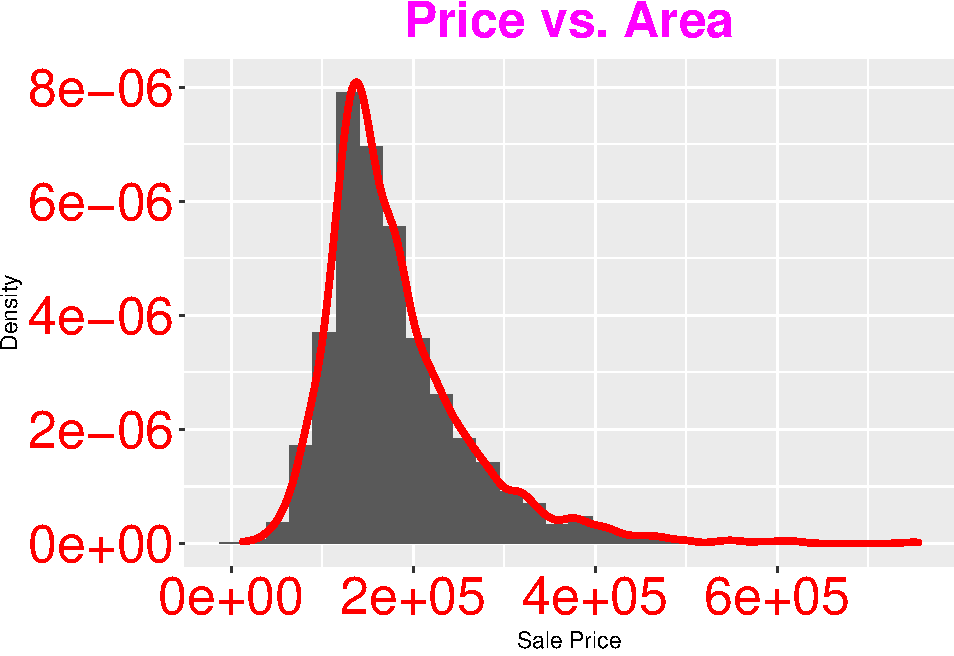
\includegraphics{04-visual_files/figure-latex/unnamed-chunk-15-1.pdf}

\hypertarget{add-lines}{%
\section{Add lines}\label{add-lines}}

Let's create some series (compounding series) of \$1000:

\begin{Shaded}
\begin{Highlighting}[]
\NormalTok{t }\OtherTok{\textless{}{-}} \FunctionTok{seq}\NormalTok{(}\DecValTok{0}\NormalTok{, }\DecValTok{10}\NormalTok{, }\DecValTok{1}\SpecialCharTok{/}\DecValTok{4}\NormalTok{)}
\NormalTok{A1 }\OtherTok{\textless{}{-}} \DecValTok{1000}\SpecialCharTok{*}\NormalTok{(}\DecValTok{1}\FloatTok{+0.05}\NormalTok{)}\SpecialCharTok{\^{}}\NormalTok{t}
\NormalTok{A2 }\OtherTok{\textless{}{-}} \DecValTok{1000}\SpecialCharTok{*}\NormalTok{(}\DecValTok{1}\FloatTok{+0.03}\NormalTok{)}\SpecialCharTok{\^{}}\NormalTok{t}
\NormalTok{A3 }\OtherTok{\textless{}{-}} \DecValTok{1000}\SpecialCharTok{*}\NormalTok{(}\DecValTok{1}\FloatTok{+0.07}\NormalTok{)}\SpecialCharTok{\^{}}\NormalTok{t}
\NormalTok{A4 }\OtherTok{\textless{}{-}} \DecValTok{1000}\SpecialCharTok{*}\NormalTok{(}\DecValTok{1}\FloatTok{+0.1}\NormalTok{)}\SpecialCharTok{\^{}}\NormalTok{t}
\end{Highlighting}
\end{Shaded}

\begin{Shaded}
\begin{Highlighting}[]
\FunctionTok{plot}\NormalTok{(t, A1)}
\end{Highlighting}
\end{Shaded}

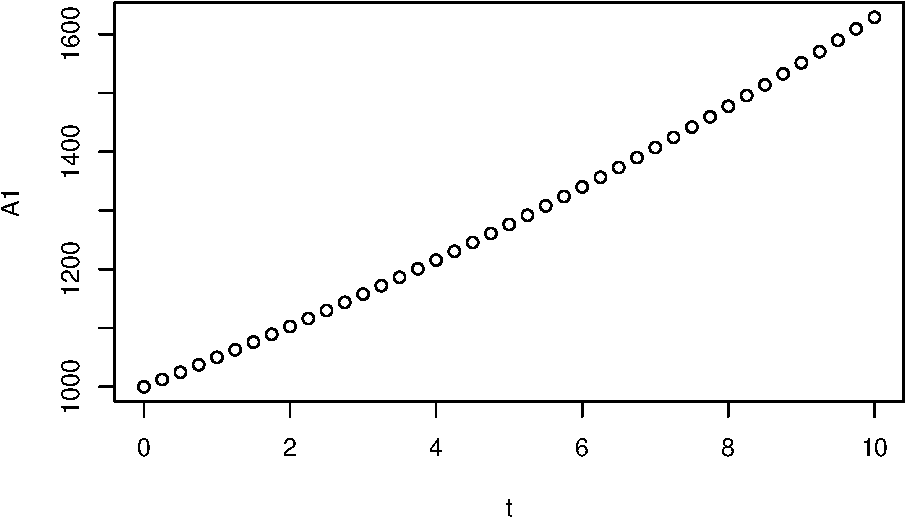
\includegraphics{04-visual_files/figure-latex/unnamed-chunk-17-1.pdf}

Here is a simple but beautiful plot \ldots{} So you may not want to use ggplot all the time:

\begin{Shaded}
\begin{Highlighting}[]
\FunctionTok{plot}\NormalTok{(t, A1,  }\AttributeTok{ylim =} \FunctionTok{c}\NormalTok{(}\DecValTok{1000}\NormalTok{,}\DecValTok{2000}\NormalTok{), }
     \AttributeTok{type =} \StringTok{"l"}\NormalTok{, }\AttributeTok{xlab =} \StringTok{"Time (in years)"}\NormalTok{, }
     \AttributeTok{ylab =} \StringTok{"Accumulated Value (in $)"}\NormalTok{, }
     \AttributeTok{main =} \StringTok{"Accumulated Value of $1000 Investment"}\NormalTok{, }\AttributeTok{col =} \StringTok{"black"}\NormalTok{)}
\FunctionTok{lines}\NormalTok{(t, A2, }\AttributeTok{type =} \StringTok{"l"}\NormalTok{, }\AttributeTok{col =} \StringTok{"blue"}\NormalTok{, }\AttributeTok{lty =} \DecValTok{2}\NormalTok{, }\AttributeTok{lwd =} \DecValTok{2}\NormalTok{)}
\FunctionTok{lines}\NormalTok{(t, A3, }\AttributeTok{type =} \StringTok{"l"}\NormalTok{, }\AttributeTok{col =} \StringTok{"red"}\NormalTok{, }\AttributeTok{lty =} \DecValTok{3}\NormalTok{, }\AttributeTok{lwd =} \DecValTok{3}\NormalTok{)}
\FunctionTok{legend}\NormalTok{(}\StringTok{"bottomright"}\NormalTok{, }
       \AttributeTok{legend =} \FunctionTok{c}\NormalTok{(}\StringTok{"3\% Interest"}\NormalTok{, }\StringTok{"5\% Interest"}\NormalTok{, }\StringTok{"7\% Interest"}\NormalTok{), }
       \AttributeTok{col =} \FunctionTok{c}\NormalTok{(}\StringTok{"blue"}\NormalTok{, }\StringTok{"black"}\NormalTok{, }\StringTok{"red"}\NormalTok{), }
       \AttributeTok{lty =} \FunctionTok{c}\NormalTok{(}\DecValTok{2}\NormalTok{, }\DecValTok{1}\NormalTok{, }\DecValTok{3}\NormalTok{), }\AttributeTok{bty =} \StringTok{"o"}\NormalTok{, }\AttributeTok{cex =} \FloatTok{0.75}\NormalTok{)}
\end{Highlighting}
\end{Shaded}

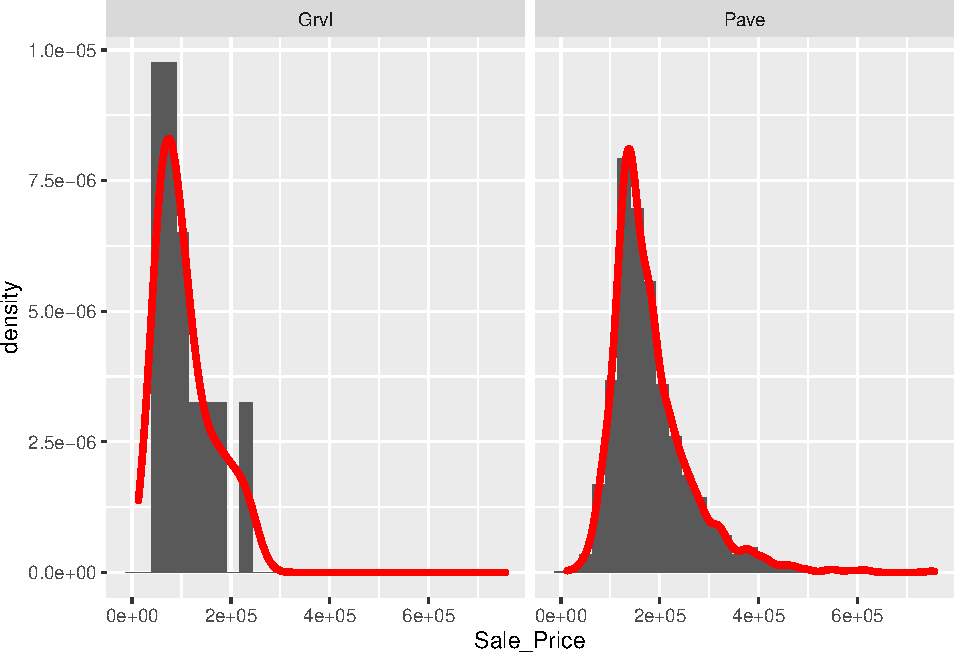
\includegraphics{04-visual_files/figure-latex/unnamed-chunk-18-1.pdf}

Or we can put them next to each other:

\begin{Shaded}
\begin{Highlighting}[]
\FunctionTok{par}\NormalTok{(}\AttributeTok{mfrow=}\FunctionTok{c}\NormalTok{(}\DecValTok{2}\NormalTok{,}\DecValTok{2}\NormalTok{), }\AttributeTok{oma =} \FunctionTok{c}\NormalTok{(}\DecValTok{0}\NormalTok{,}\DecValTok{0}\NormalTok{,}\DecValTok{2}\NormalTok{,}\DecValTok{0}\NormalTok{)) }\CommentTok{\# puts 4 plots in one window (2x2)}

\FunctionTok{plot}\NormalTok{(t, A1, }\AttributeTok{type =} \StringTok{"l"}\NormalTok{, }\AttributeTok{xlab =} \StringTok{"Time (in years)"}\NormalTok{, }
     \AttributeTok{ylab =} \StringTok{"AV {-} $"}\NormalTok{, }\AttributeTok{ylim =} \FunctionTok{c}\NormalTok{(}\DecValTok{1000}\NormalTok{, }\DecValTok{2500}\NormalTok{),}
     \AttributeTok{main =} \StringTok{"(i = 0.05)"}\NormalTok{)}

\FunctionTok{plot}\NormalTok{(t, A2, }\AttributeTok{type =} \StringTok{"l"}\NormalTok{, }\AttributeTok{xlab =} \StringTok{"Time (in years)"}\NormalTok{, }
     \AttributeTok{ylab =} \StringTok{"AV {-} $"}\NormalTok{, }\AttributeTok{ylim =} \FunctionTok{c}\NormalTok{(}\DecValTok{1000}\NormalTok{, }\DecValTok{2500}\NormalTok{),}
     \AttributeTok{main =} \StringTok{"(i = 0.03)"}\NormalTok{)}

\FunctionTok{plot}\NormalTok{(t, A3, }\AttributeTok{type =} \StringTok{"l"}\NormalTok{, }\AttributeTok{xlab =} \StringTok{"Time (in years)"}\NormalTok{, }
     \AttributeTok{ylab =} \StringTok{"AV {-} $"}\NormalTok{, }\AttributeTok{ylim =} \FunctionTok{c}\NormalTok{(}\DecValTok{1000}\NormalTok{, }\DecValTok{2500}\NormalTok{),}
     \AttributeTok{main =} \StringTok{"(i = 0.07)"}\NormalTok{)}

\FunctionTok{plot}\NormalTok{(t, A4, }\AttributeTok{type =} \StringTok{"l"}\NormalTok{, }\AttributeTok{xlab =} \StringTok{"Time (in years)"}\NormalTok{, }
     \AttributeTok{ylab =} \StringTok{"AV {-} $"}\NormalTok{, }\AttributeTok{ylim =} \FunctionTok{c}\NormalTok{(}\DecValTok{1000}\NormalTok{, }\DecValTok{2500}\NormalTok{),}
     \AttributeTok{main =} \StringTok{"(i = 0.1)"}\NormalTok{)}

\FunctionTok{mtext}\NormalTok{(}\StringTok{"Accumulated Value of $1000 Investment"}\NormalTok{,}
      \AttributeTok{outer=}\ConstantTok{TRUE}\NormalTok{, }\AttributeTok{cex =} \FloatTok{1.5}\NormalTok{, }\AttributeTok{col=}\StringTok{"olivedrab"}\NormalTok{)}
\end{Highlighting}
\end{Shaded}

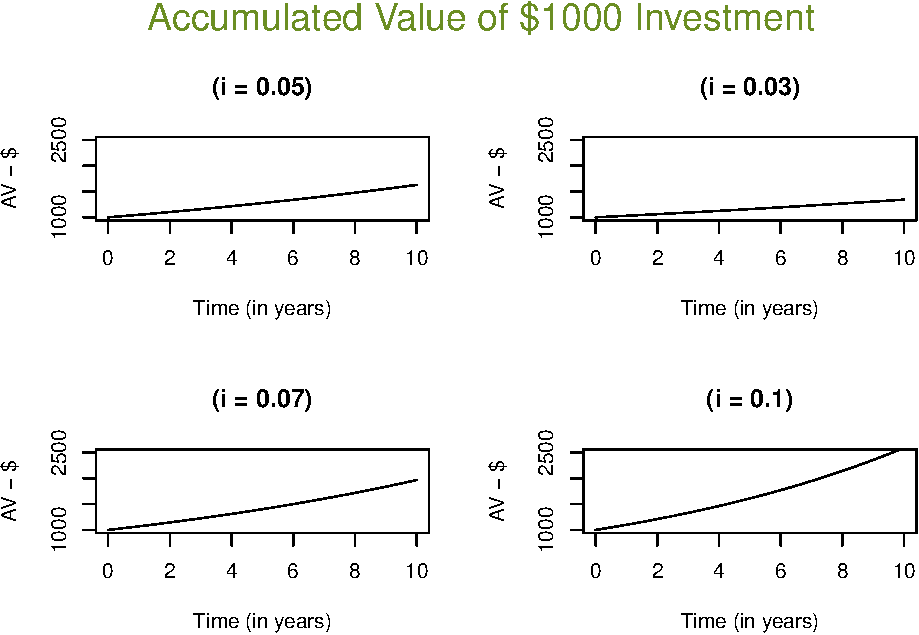
\includegraphics{04-visual_files/figure-latex/unnamed-chunk-19-1.pdf}

\hypertarget{pairwise-relationship}{%
\section{Pairwise relationship}\label{pairwise-relationship}}

R package \texttt{corrplot} provides a visual exploratory tool on correlation matrix that supports automatic variable reordering to help detect hidden patterns among variables. See more details \href{https://cran.r-project.org/web/packages/corrplot/vignettes/corrplot-intro.html}{here}

\begin{Shaded}
\begin{Highlighting}[]
\FunctionTok{library}\NormalTok{(corrplot)}
\end{Highlighting}
\end{Shaded}

\begin{verbatim}
## corrplot 0.92 loaded
\end{verbatim}

\begin{Shaded}
\begin{Highlighting}[]
\NormalTok{M }\OtherTok{=} \FunctionTok{cor}\NormalTok{(mtcars)}
\FunctionTok{corrplot}\NormalTok{(M, }\AttributeTok{method =} \StringTok{\textquotesingle{}number\textquotesingle{}}\NormalTok{) }\CommentTok{\# colorful number}
\end{Highlighting}
\end{Shaded}

\includegraphics{04-visual_files/figure-latex/unnamed-chunk-20-1.pdf}

\begin{Shaded}
\begin{Highlighting}[]
\FunctionTok{corrplot}\NormalTok{(M)}
\end{Highlighting}
\end{Shaded}

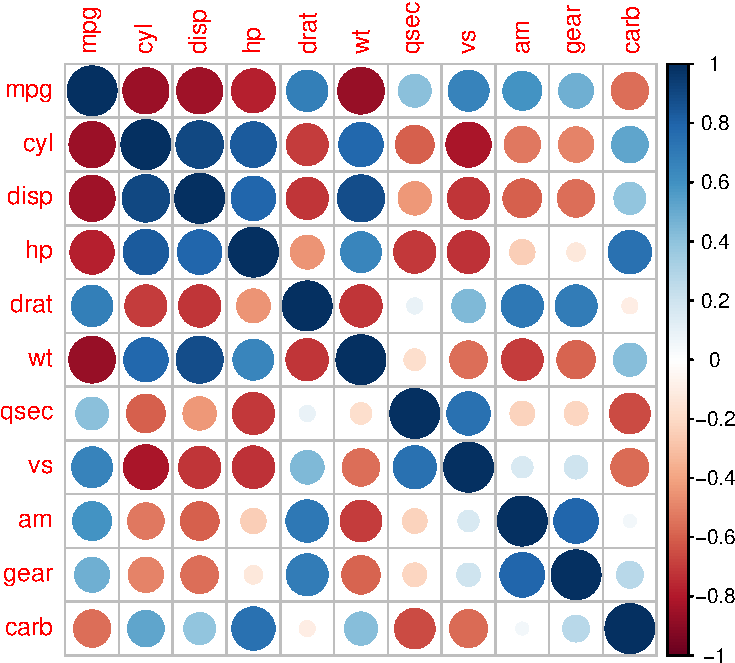
\includegraphics{04-visual_files/figure-latex/unnamed-chunk-20-2.pdf}

\begin{Shaded}
\begin{Highlighting}[]
\FunctionTok{corrplot}\NormalTok{(M, }\AttributeTok{order =} \StringTok{\textquotesingle{}AOE\textquotesingle{}}\NormalTok{)}
\end{Highlighting}
\end{Shaded}

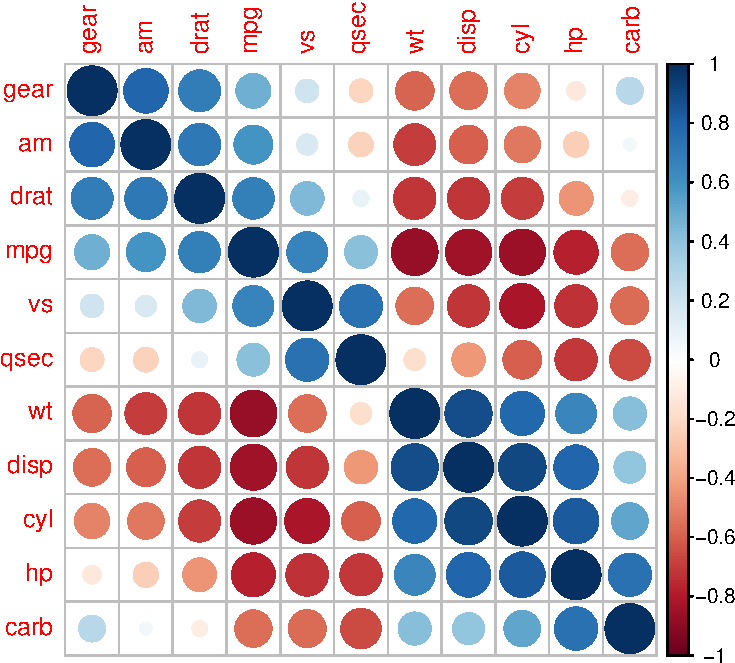
\includegraphics{04-visual_files/figure-latex/unnamed-chunk-20-3.pdf}

\begin{Shaded}
\begin{Highlighting}[]
\FunctionTok{corrplot.mixed}\NormalTok{(M, }\AttributeTok{order =} \StringTok{\textquotesingle{}AOE\textquotesingle{}}\NormalTok{)}
\end{Highlighting}
\end{Shaded}

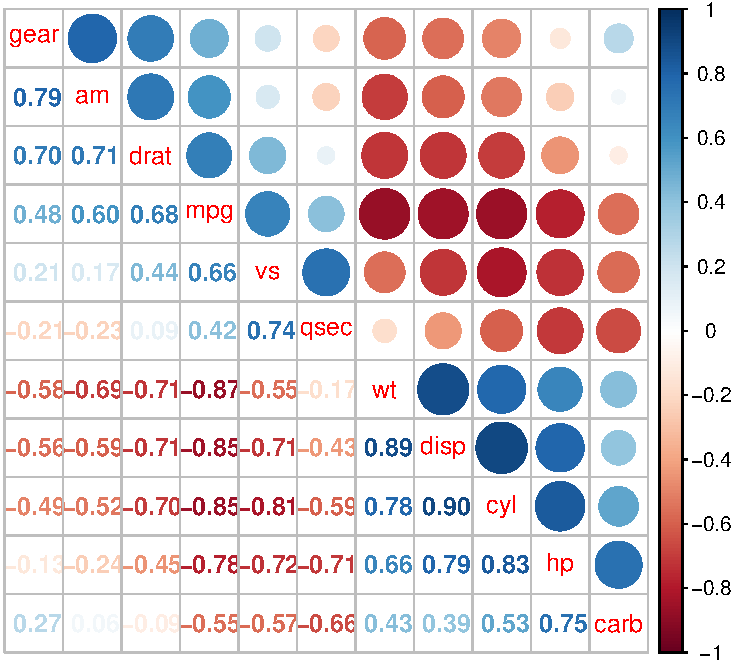
\includegraphics{04-visual_files/figure-latex/unnamed-chunk-20-4.pdf}

\hypertarget{conditional-scatterplot}{%
\section{Conditional Scatterplot}\label{conditional-scatterplot}}

To visualize the relationship between two continuous variables but for different levels of a factor variable you can create a conditional scatterplot with \texttt{coplot()}. Note that we haven't converted \texttt{maturity.stage} to a factor variable.

\begin{Shaded}
\begin{Highlighting}[]
\FunctionTok{library}\NormalTok{(RBootcamp)}
\FunctionTok{coplot}\NormalTok{(weight }\SpecialCharTok{\textasciitilde{}}\NormalTok{ DML }\SpecialCharTok{|}\NormalTok{ maturity.stage, }\AttributeTok{data =}\NormalTok{ squid1)}
\end{Highlighting}
\end{Shaded}

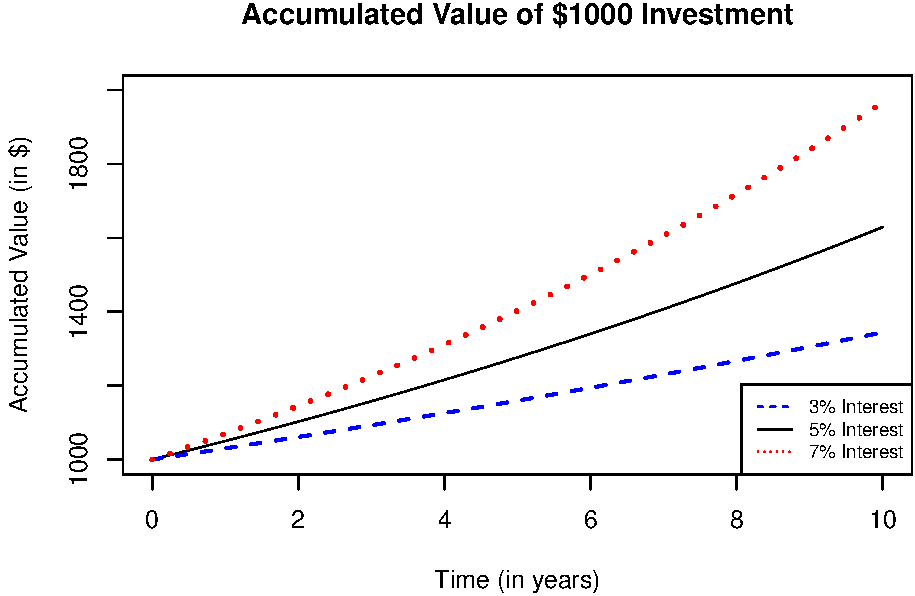
\includegraphics{04-visual_files/figure-latex/unnamed-chunk-21-1.pdf}

\hypertarget{panel}{%
\section{\texorpdfstring{\texttt{panel()}}{panel()}}\label{panel}}

To explore the relationships between multiple continuous variables we can have a pairs plot.

\begin{Shaded}
\begin{Highlighting}[]
\FunctionTok{pairs}\NormalTok{(mtcars[, }\FunctionTok{c}\NormalTok{(}\DecValTok{1}\NormalTok{, }\DecValTok{3}\NormalTok{, }\DecValTok{6}\NormalTok{)])}
\end{Highlighting}
\end{Shaded}

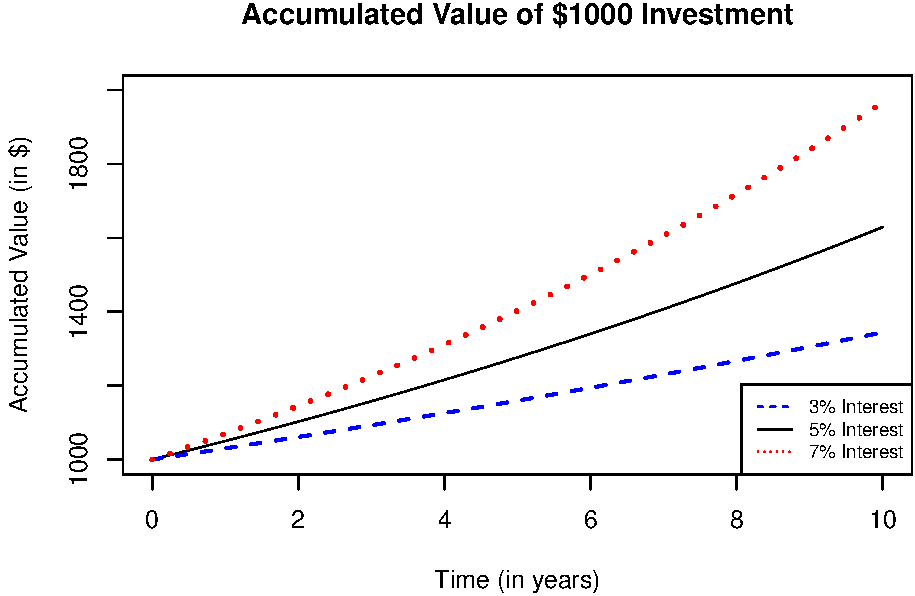
\includegraphics{04-visual_files/figure-latex/unnamed-chunk-22-1.pdf}

\hypertarget{data-management}{%
\chapter{Data Management}\label{data-management}}

We will use the same data set, Ames Housing Price data from the \texttt{AmesHousing} package, containing 2930 observations and 81 features including the sale date and price. And we will introduce the \texttt{dplyr} package in many applications. See more about \texttt{dplyr} \href{https://dplyr.tidyverse.org/articles/dplyr.html}{here}

\begin{Shaded}
\begin{Highlighting}[]
\FunctionTok{library}\NormalTok{(AmesHousing)}
\FunctionTok{library}\NormalTok{(dplyr)}
\end{Highlighting}
\end{Shaded}

\begin{verbatim}
## 
## Attaching package: 'dplyr'
\end{verbatim}

\begin{verbatim}
## The following objects are masked from 'package:stats':
## 
##     filter, lag
\end{verbatim}

\begin{verbatim}
## The following objects are masked from 'package:base':
## 
##     intersect, setdiff, setequal, union
\end{verbatim}

\begin{Shaded}
\begin{Highlighting}[]
\NormalTok{amesdata }\OtherTok{\textless{}{-}} \FunctionTok{make\_ames}\NormalTok{()}
\FunctionTok{glimpse}\NormalTok{(amesdata)}
\end{Highlighting}
\end{Shaded}

\begin{verbatim}
## Rows: 2,930
## Columns: 81
## $ MS_SubClass        <fct> One_Story_1946_and_Newer_All_Styles, One_Story_1946~
## $ MS_Zoning          <fct> Residential_Low_Density, Residential_High_Density, ~
## $ Lot_Frontage       <dbl> 141, 80, 81, 93, 74, 78, 41, 43, 39, 60, 75, 0, 63,~
## $ Lot_Area           <int> 31770, 11622, 14267, 11160, 13830, 9978, 4920, 5005~
## $ Street             <fct> Pave, Pave, Pave, Pave, Pave, Pave, Pave, Pave, Pav~
## $ Alley              <fct> No_Alley_Access, No_Alley_Access, No_Alley_Access, ~
## $ Lot_Shape          <fct> Slightly_Irregular, Regular, Slightly_Irregular, Re~
## $ Land_Contour       <fct> Lvl, Lvl, Lvl, Lvl, Lvl, Lvl, Lvl, HLS, Lvl, Lvl, L~
## $ Utilities          <fct> AllPub, AllPub, AllPub, AllPub, AllPub, AllPub, All~
## $ Lot_Config         <fct> Corner, Inside, Corner, Corner, Inside, Inside, Ins~
## $ Land_Slope         <fct> Gtl, Gtl, Gtl, Gtl, Gtl, Gtl, Gtl, Gtl, Gtl, Gtl, G~
## $ Neighborhood       <fct> North_Ames, North_Ames, North_Ames, North_Ames, Gil~
## $ Condition_1        <fct> Norm, Feedr, Norm, Norm, Norm, Norm, Norm, Norm, No~
## $ Condition_2        <fct> Norm, Norm, Norm, Norm, Norm, Norm, Norm, Norm, Nor~
## $ Bldg_Type          <fct> OneFam, OneFam, OneFam, OneFam, OneFam, OneFam, Twn~
## $ House_Style        <fct> One_Story, One_Story, One_Story, One_Story, Two_Sto~
## $ Overall_Qual       <fct> Above_Average, Average, Above_Average, Good, Averag~
## $ Overall_Cond       <fct> Average, Above_Average, Above_Average, Average, Ave~
## $ Year_Built         <int> 1960, 1961, 1958, 1968, 1997, 1998, 2001, 1992, 199~
## $ Year_Remod_Add     <int> 1960, 1961, 1958, 1968, 1998, 1998, 2001, 1992, 199~
## $ Roof_Style         <fct> Hip, Gable, Hip, Hip, Gable, Gable, Gable, Gable, G~
## $ Roof_Matl          <fct> CompShg, CompShg, CompShg, CompShg, CompShg, CompSh~
## $ Exterior_1st       <fct> BrkFace, VinylSd, Wd Sdng, BrkFace, VinylSd, VinylS~
## $ Exterior_2nd       <fct> Plywood, VinylSd, Wd Sdng, BrkFace, VinylSd, VinylS~
## $ Mas_Vnr_Type       <fct> Stone, None, BrkFace, None, None, BrkFace, None, No~
## $ Mas_Vnr_Area       <dbl> 112, 0, 108, 0, 0, 20, 0, 0, 0, 0, 0, 0, 0, 0, 0, 6~
## $ Exter_Qual         <fct> Typical, Typical, Typical, Good, Typical, Typical, ~
## $ Exter_Cond         <fct> Typical, Typical, Typical, Typical, Typical, Typica~
## $ Foundation         <fct> CBlock, CBlock, CBlock, CBlock, PConc, PConc, PConc~
## $ Bsmt_Qual          <fct> Typical, Typical, Typical, Typical, Good, Typical, ~
## $ Bsmt_Cond          <fct> Good, Typical, Typical, Typical, Typical, Typical, ~
## $ Bsmt_Exposure      <fct> Gd, No, No, No, No, No, Mn, No, No, No, No, No, No,~
## $ BsmtFin_Type_1     <fct> BLQ, Rec, ALQ, ALQ, GLQ, GLQ, GLQ, ALQ, GLQ, Unf, U~
## $ BsmtFin_SF_1       <dbl> 2, 6, 1, 1, 3, 3, 3, 1, 3, 7, 7, 1, 7, 3, 3, 1, 3, ~
## $ BsmtFin_Type_2     <fct> Unf, LwQ, Unf, Unf, Unf, Unf, Unf, Unf, Unf, Unf, U~
## $ BsmtFin_SF_2       <dbl> 0, 144, 0, 0, 0, 0, 0, 0, 0, 0, 0, 0, 0, 0, 1120, 0~
## $ Bsmt_Unf_SF        <dbl> 441, 270, 406, 1045, 137, 324, 722, 1017, 415, 994,~
## $ Total_Bsmt_SF      <dbl> 1080, 882, 1329, 2110, 928, 926, 1338, 1280, 1595, ~
## $ Heating            <fct> GasA, GasA, GasA, GasA, GasA, GasA, GasA, GasA, Gas~
## $ Heating_QC         <fct> Fair, Typical, Typical, Excellent, Good, Excellent,~
## $ Central_Air        <fct> Y, Y, Y, Y, Y, Y, Y, Y, Y, Y, Y, Y, Y, Y, Y, Y, Y, ~
## $ Electrical         <fct> SBrkr, SBrkr, SBrkr, SBrkr, SBrkr, SBrkr, SBrkr, SB~
## $ First_Flr_SF       <int> 1656, 896, 1329, 2110, 928, 926, 1338, 1280, 1616, ~
## $ Second_Flr_SF      <int> 0, 0, 0, 0, 701, 678, 0, 0, 0, 776, 892, 0, 676, 0,~
## $ Low_Qual_Fin_SF    <int> 0, 0, 0, 0, 0, 0, 0, 0, 0, 0, 0, 0, 0, 0, 0, 0, 0, ~
## $ Gr_Liv_Area        <int> 1656, 896, 1329, 2110, 1629, 1604, 1338, 1280, 1616~
## $ Bsmt_Full_Bath     <dbl> 1, 0, 0, 1, 0, 0, 1, 0, 1, 0, 0, 1, 0, 1, 1, 1, 0, ~
## $ Bsmt_Half_Bath     <dbl> 0, 0, 0, 0, 0, 0, 0, 0, 0, 0, 0, 0, 0, 0, 0, 0, 0, ~
## $ Full_Bath          <int> 1, 1, 1, 2, 2, 2, 2, 2, 2, 2, 2, 2, 2, 1, 1, 3, 2, ~
## $ Half_Bath          <int> 0, 0, 1, 1, 1, 1, 0, 0, 0, 1, 1, 0, 1, 1, 1, 1, 0, ~
## $ Bedroom_AbvGr      <int> 3, 2, 3, 3, 3, 3, 2, 2, 2, 3, 3, 3, 3, 2, 1, 4, 4, ~
## $ Kitchen_AbvGr      <int> 1, 1, 1, 1, 1, 1, 1, 1, 1, 1, 1, 1, 1, 1, 1, 1, 1, ~
## $ Kitchen_Qual       <fct> Typical, Typical, Good, Excellent, Typical, Good, G~
## $ TotRms_AbvGrd      <int> 7, 5, 6, 8, 6, 7, 6, 5, 5, 7, 7, 6, 7, 5, 4, 12, 8,~
## $ Functional         <fct> Typ, Typ, Typ, Typ, Typ, Typ, Typ, Typ, Typ, Typ, T~
## $ Fireplaces         <int> 2, 0, 0, 2, 1, 1, 0, 0, 1, 1, 1, 0, 1, 1, 0, 1, 0, ~
## $ Fireplace_Qu       <fct> Good, No_Fireplace, No_Fireplace, Typical, Typical,~
## $ Garage_Type        <fct> Attchd, Attchd, Attchd, Attchd, Attchd, Attchd, Att~
## $ Garage_Finish      <fct> Fin, Unf, Unf, Fin, Fin, Fin, Fin, RFn, RFn, Fin, F~
## $ Garage_Cars        <dbl> 2, 1, 1, 2, 2, 2, 2, 2, 2, 2, 2, 2, 2, 2, 2, 3, 2, ~
## $ Garage_Area        <dbl> 528, 730, 312, 522, 482, 470, 582, 506, 608, 442, 4~
## $ Garage_Qual        <fct> Typical, Typical, Typical, Typical, Typical, Typica~
## $ Garage_Cond        <fct> Typical, Typical, Typical, Typical, Typical, Typica~
## $ Paved_Drive        <fct> Partial_Pavement, Paved, Paved, Paved, Paved, Paved~
## $ Wood_Deck_SF       <int> 210, 140, 393, 0, 212, 360, 0, 0, 237, 140, 157, 48~
## $ Open_Porch_SF      <int> 62, 0, 36, 0, 34, 36, 0, 82, 152, 60, 84, 21, 75, 0~
## $ Enclosed_Porch     <int> 0, 0, 0, 0, 0, 0, 170, 0, 0, 0, 0, 0, 0, 0, 0, 0, 0~
## $ Three_season_porch <int> 0, 0, 0, 0, 0, 0, 0, 0, 0, 0, 0, 0, 0, 0, 0, 0, 0, ~
## $ Screen_Porch       <int> 0, 120, 0, 0, 0, 0, 0, 144, 0, 0, 0, 0, 0, 0, 140, ~
## $ Pool_Area          <int> 0, 0, 0, 0, 0, 0, 0, 0, 0, 0, 0, 0, 0, 0, 0, 0, 0, ~
## $ Pool_QC            <fct> No_Pool, No_Pool, No_Pool, No_Pool, No_Pool, No_Poo~
## $ Fence              <fct> No_Fence, Minimum_Privacy, No_Fence, No_Fence, Mini~
## $ Misc_Feature       <fct> None, None, Gar2, None, None, None, None, None, Non~
## $ Misc_Val           <int> 0, 0, 12500, 0, 0, 0, 0, 0, 0, 0, 0, 500, 0, 0, 0, ~
## $ Mo_Sold            <int> 5, 6, 6, 4, 3, 6, 4, 1, 3, 6, 4, 3, 5, 2, 6, 6, 6, ~
## $ Year_Sold          <int> 2010, 2010, 2010, 2010, 2010, 2010, 2010, 2010, 201~
## $ Sale_Type          <fct> WD , WD , WD , WD , WD , WD , WD , WD , WD , WD , W~
## $ Sale_Condition     <fct> Normal, Normal, Normal, Normal, Normal, Normal, Nor~
## $ Sale_Price         <int> 215000, 105000, 172000, 244000, 189900, 195500, 213~
## $ Longitude          <dbl> -93.61975, -93.61976, -93.61939, -93.61732, -93.638~
## $ Latitude           <dbl> 42.05403, 42.05301, 42.05266, 42.05125, 42.06090, 4~
\end{verbatim}

\hypertarget{filter}{%
\section{Filter}\label{filter}}

Suppose we want to find the houses that are sold in Jan 2010. You can use the function \texttt{filter()} in the \texttt{dplyr} package, a member of the tidyverse package. We can use subsetting operations

\begin{Shaded}
\begin{Highlighting}[]
\NormalTok{amesdata[amesdata}\SpecialCharTok{$}\NormalTok{Year\_Sold }\SpecialCharTok{==} \DecValTok{2010} \SpecialCharTok{\&}\NormalTok{ amesdata}\SpecialCharTok{$}\NormalTok{Mo\_Sold }\SpecialCharTok{==} \DecValTok{1}\NormalTok{, ] }
\end{Highlighting}
\end{Shaded}

\begin{verbatim}
## # A tibble: 26 x 81
##    MS_Sub~1 MS_Zo~2 Lot_F~3 Lot_A~4 Street Alley Lot_S~5 Land_~6 Utili~7 Lot_C~8
##    <fct>    <fct>     <dbl>   <int> <fct>  <fct> <fct>   <fct>   <fct>   <fct>  
##  1 One_Sto~ Reside~      43    5005 Pave   No_A~ Slight~ HLS     AllPub  Inside 
##  2 One_Sto~ Reside~     105   11751 Pave   No_A~ Slight~ Lvl     AllPub  Inside 
##  3 Split_F~ Reside~      85   10625 Pave   No_A~ Regular Lvl     AllPub  Inside 
##  4 Two_Sto~ Floati~       0    7500 Pave   No_A~ Regular Lvl     AllPub  Inside 
##  5 Two_Sto~ Reside~     102   12858 Pave   No_A~ Slight~ Lvl     AllPub  Inside 
##  6 One_Sto~ Reside~     100   18494 Pave   No_A~ Slight~ Lvl     AllPub  Corner 
##  7 One_Sto~ Reside~      43    3203 Pave   No_A~ Regular Lvl     AllPub  Inside 
##  8 Two_Sto~ Reside~      60   17433 Pave   No_A~ Modera~ Lvl     AllPub  CulDSac
##  9 Two_Sto~ Reside~      76   10142 Pave   No_A~ Slight~ Lvl     AllPub  Inside 
## 10 Two_Sto~ Floati~      39    3515 Pave   Paved Regular Lvl     AllPub  Inside 
## # ... with 16 more rows, 71 more variables: Land_Slope <fct>,
## #   Neighborhood <fct>, Condition_1 <fct>, Condition_2 <fct>, Bldg_Type <fct>,
## #   House_Style <fct>, Overall_Qual <fct>, Overall_Cond <fct>,
## #   Year_Built <int>, Year_Remod_Add <int>, Roof_Style <fct>, Roof_Matl <fct>,
## #   Exterior_1st <fct>, Exterior_2nd <fct>, Mas_Vnr_Type <fct>,
## #   Mas_Vnr_Area <dbl>, Exter_Qual <fct>, Exter_Cond <fct>, Foundation <fct>,
## #   Bsmt_Qual <fct>, Bsmt_Cond <fct>, Bsmt_Exposure <fct>, ...
\end{verbatim}

Or we can use \texttt{filter()}:

\begin{Shaded}
\begin{Highlighting}[]
\FunctionTok{library}\NormalTok{(dplyr)}
\NormalTok{dplyr}\SpecialCharTok{::}\FunctionTok{filter}\NormalTok{(amesdata, Year\_Sold }\SpecialCharTok{==} \DecValTok{2010}\NormalTok{, Mo\_Sold }\SpecialCharTok{==} \DecValTok{1}\NormalTok{)}
\end{Highlighting}
\end{Shaded}

\begin{verbatim}
## # A tibble: 26 x 81
##    MS_Sub~1 MS_Zo~2 Lot_F~3 Lot_A~4 Street Alley Lot_S~5 Land_~6 Utili~7 Lot_C~8
##    <fct>    <fct>     <dbl>   <int> <fct>  <fct> <fct>   <fct>   <fct>   <fct>  
##  1 One_Sto~ Reside~      43    5005 Pave   No_A~ Slight~ HLS     AllPub  Inside 
##  2 One_Sto~ Reside~     105   11751 Pave   No_A~ Slight~ Lvl     AllPub  Inside 
##  3 Split_F~ Reside~      85   10625 Pave   No_A~ Regular Lvl     AllPub  Inside 
##  4 Two_Sto~ Floati~       0    7500 Pave   No_A~ Regular Lvl     AllPub  Inside 
##  5 Two_Sto~ Reside~     102   12858 Pave   No_A~ Slight~ Lvl     AllPub  Inside 
##  6 One_Sto~ Reside~     100   18494 Pave   No_A~ Slight~ Lvl     AllPub  Corner 
##  7 One_Sto~ Reside~      43    3203 Pave   No_A~ Regular Lvl     AllPub  Inside 
##  8 Two_Sto~ Reside~      60   17433 Pave   No_A~ Modera~ Lvl     AllPub  CulDSac
##  9 Two_Sto~ Reside~      76   10142 Pave   No_A~ Slight~ Lvl     AllPub  Inside 
## 10 Two_Sto~ Floati~      39    3515 Pave   Paved Regular Lvl     AllPub  Inside 
## # ... with 16 more rows, 71 more variables: Land_Slope <fct>,
## #   Neighborhood <fct>, Condition_1 <fct>, Condition_2 <fct>, Bldg_Type <fct>,
## #   House_Style <fct>, Overall_Qual <fct>, Overall_Cond <fct>,
## #   Year_Built <int>, Year_Remod_Add <int>, Roof_Style <fct>, Roof_Matl <fct>,
## #   Exterior_1st <fct>, Exterior_2nd <fct>, Mas_Vnr_Type <fct>,
## #   Mas_Vnr_Area <dbl>, Exter_Qual <fct>, Exter_Cond <fct>, Foundation <fct>,
## #   Bsmt_Qual <fct>, Bsmt_Cond <fct>, Bsmt_Exposure <fct>, ...
\end{verbatim}

\hypertarget{arrange}{%
\section{Arrange}\label{arrange}}

Let's find the 10 houses with the highest sale prices by year

\begin{Shaded}
\begin{Highlighting}[]
\NormalTok{ar }\OtherTok{\textless{}{-}} \FunctionTok{arrange}\NormalTok{(amesdata, Year\_Sold, }\FunctionTok{desc}\NormalTok{(Sale\_Price))}
\NormalTok{ar}
\end{Highlighting}
\end{Shaded}

\begin{verbatim}
## # A tibble: 2,930 x 81
##    MS_Sub~1 MS_Zo~2 Lot_F~3 Lot_A~4 Street Alley Lot_S~5 Land_~6 Utili~7 Lot_C~8
##    <fct>    <fct>     <dbl>   <int> <fct>  <fct> <fct>   <fct>   <fct>   <fct>  
##  1 Two_Sto~ Reside~     118   35760 Pave   No_A~ Slight~ Lvl     AllPub  CulDSac
##  2 Two_Sto~ Reside~     114   17242 Pave   No_A~ Slight~ Lvl     AllPub  Inside 
##  3 Two_Sto~ Reside~      85   16056 Pave   No_A~ Slight~ Lvl     AllPub  Inside 
##  4 Two_Sto~ Reside~      60   18062 Pave   No_A~ Slight~ HLS     AllPub  CulDSac
##  5 Two_Sto~ Reside~      82   16052 Pave   No_A~ Slight~ Lvl     AllPub  CulDSac
##  6 Two_and~ Reside~      90   22950 Pave   No_A~ Modera~ Lvl     AllPub  Inside 
##  7 One_Sto~ Reside~      90   18261 Pave   No_A~ Slight~ HLS     AllPub  Inside 
##  8 One_Sto~ Reside~     107   13891 Pave   No_A~ Regular Lvl     AllPub  Inside 
##  9 Two_Sto~ Reside~      59   16023 Pave   No_A~ Slight~ HLS     AllPub  CulDSac
## 10 Two_Sto~ Reside~      66   13682 Pave   No_A~ Modera~ HLS     AllPub  CulDSac
## # ... with 2,920 more rows, 71 more variables: Land_Slope <fct>,
## #   Neighborhood <fct>, Condition_1 <fct>, Condition_2 <fct>, Bldg_Type <fct>,
## #   House_Style <fct>, Overall_Qual <fct>, Overall_Cond <fct>,
## #   Year_Built <int>, Year_Remod_Add <int>, Roof_Style <fct>, Roof_Matl <fct>,
## #   Exterior_1st <fct>, Exterior_2nd <fct>, Mas_Vnr_Type <fct>,
## #   Mas_Vnr_Area <dbl>, Exter_Qual <fct>, Exter_Cond <fct>, Foundation <fct>,
## #   Bsmt_Qual <fct>, Bsmt_Cond <fct>, Bsmt_Exposure <fct>, ...
\end{verbatim}

Or

\begin{Shaded}
\begin{Highlighting}[]
\NormalTok{arr }\OtherTok{\textless{}{-}}\NormalTok{ amesdata[}\FunctionTok{order}\NormalTok{(amesdata}\SpecialCharTok{$}\NormalTok{Year\_Sold, }\FunctionTok{desc}\NormalTok{(amesdata}\SpecialCharTok{$}\NormalTok{Sale\_Price)), ]}
\FunctionTok{head}\NormalTok{(arr)}
\end{Highlighting}
\end{Shaded}

\begin{verbatim}
## # A tibble: 6 x 81
##   MS_SubC~1 MS_Zo~2 Lot_F~3 Lot_A~4 Street Alley Lot_S~5 Land_~6 Utili~7 Lot_C~8
##   <fct>     <fct>     <dbl>   <int> <fct>  <fct> <fct>   <fct>   <fct>   <fct>  
## 1 Two_Stor~ Reside~     118   35760 Pave   No_A~ Slight~ Lvl     AllPub  CulDSac
## 2 Two_Stor~ Reside~     114   17242 Pave   No_A~ Slight~ Lvl     AllPub  Inside 
## 3 Two_Stor~ Reside~      85   16056 Pave   No_A~ Slight~ Lvl     AllPub  Inside 
## 4 Two_Stor~ Reside~      60   18062 Pave   No_A~ Slight~ HLS     AllPub  CulDSac
## 5 Two_Stor~ Reside~      82   16052 Pave   No_A~ Slight~ Lvl     AllPub  CulDSac
## 6 Two_and_~ Reside~      90   22950 Pave   No_A~ Modera~ Lvl     AllPub  Inside 
## # ... with 71 more variables: Land_Slope <fct>, Neighborhood <fct>,
## #   Condition_1 <fct>, Condition_2 <fct>, Bldg_Type <fct>, House_Style <fct>,
## #   Overall_Qual <fct>, Overall_Cond <fct>, Year_Built <int>,
## #   Year_Remod_Add <int>, Roof_Style <fct>, Roof_Matl <fct>,
## #   Exterior_1st <fct>, Exterior_2nd <fct>, Mas_Vnr_Type <fct>,
## #   Mas_Vnr_Area <dbl>, Exter_Qual <fct>, Exter_Cond <fct>, Foundation <fct>,
## #   Bsmt_Qual <fct>, Bsmt_Cond <fct>, Bsmt_Exposure <fct>, ...
\end{verbatim}

\hypertarget{pipe}{%
\section{Pipe}\label{pipe}}

Pipes help us apply multiple operations sequentially on a given data.

\begin{Shaded}
\begin{Highlighting}[]
\FunctionTok{library}\NormalTok{(ggplot2)}
\NormalTok{amesdata }\SpecialCharTok{\%\textgreater{}\%} 
  \FunctionTok{filter}\NormalTok{(Year\_Sold }\SpecialCharTok{==} \DecValTok{2009}\NormalTok{, Mo\_Sold }\SpecialCharTok{==} \DecValTok{1}\NormalTok{) }\SpecialCharTok{\%\textgreater{}\%} 
  \FunctionTok{arrange}\NormalTok{(Year\_Built) }\SpecialCharTok{\%\textgreater{}\%}
  \FunctionTok{ggplot}\NormalTok{(}\AttributeTok{mapping =} \FunctionTok{aes}\NormalTok{(}\AttributeTok{x =}\NormalTok{ Lot\_Area, }\AttributeTok{y =}\NormalTok{ Sale\_Price)) }\SpecialCharTok{+} 
  \FunctionTok{geom\_point}\NormalTok{()}
\end{Highlighting}
\end{Shaded}

\includegraphics{05-DataMan_files/figure-latex/unnamed-chunk-6-1.pdf}

\hypertarget{select}{%
\section{Select}\label{select}}

How do we select variables based on some characteristics

\begin{Shaded}
\begin{Highlighting}[]
\NormalTok{amesdata }\SpecialCharTok{\%\textgreater{}\%} \FunctionTok{select}\NormalTok{(}\FunctionTok{starts\_with}\NormalTok{(}\StringTok{"Year"}\NormalTok{), Sale\_Price)}
\end{Highlighting}
\end{Shaded}

\begin{verbatim}
## # A tibble: 2,930 x 4
##    Year_Built Year_Remod_Add Year_Sold Sale_Price
##         <int>          <int>     <int>      <int>
##  1       1960           1960      2010     215000
##  2       1961           1961      2010     105000
##  3       1958           1958      2010     172000
##  4       1968           1968      2010     244000
##  5       1997           1998      2010     189900
##  6       1998           1998      2010     195500
##  7       2001           2001      2010     213500
##  8       1992           1992      2010     191500
##  9       1995           1996      2010     236500
## 10       1999           1999      2010     189000
## # ... with 2,920 more rows
\end{verbatim}

\begin{Shaded}
\begin{Highlighting}[]
\NormalTok{amesdata }\SpecialCharTok{\%\textgreater{}\%} \FunctionTok{select}\NormalTok{(}\FunctionTok{contains}\NormalTok{(}\StringTok{"Mo"}\NormalTok{))}
\end{Highlighting}
\end{Shaded}

\begin{verbatim}
## # A tibble: 2,930 x 2
##    Year_Remod_Add Mo_Sold
##             <int>   <int>
##  1           1960       5
##  2           1961       6
##  3           1958       6
##  4           1968       4
##  5           1998       3
##  6           1998       6
##  7           2001       4
##  8           1992       1
##  9           1996       3
## 10           1999       6
## # ... with 2,920 more rows
\end{verbatim}

\hypertarget{create-group_by}{%
\section{\texorpdfstring{Create \& \texttt{group\_by()}}{Create \& group\_by()}}\label{create-group_by}}

We may want to create new variables as functions of the existing ones by \texttt{mutate()}:

\begin{Shaded}
\begin{Highlighting}[]
\FunctionTok{library}\NormalTok{(r02pro)}
\FunctionTok{library}\NormalTok{(tidyverse)}
\NormalTok{amesdata }\SpecialCharTok{\%\textgreater{}\%} 
  \FunctionTok{select}\NormalTok{(Overall\_Qual, Lot\_Area, Sale\_Price) }\SpecialCharTok{\%\textgreater{}\%}
  \FunctionTok{mutate}\NormalTok{(}\AttributeTok{ave\_price =}\NormalTok{ Sale\_Price}\SpecialCharTok{/}\NormalTok{Lot\_Area) }
\end{Highlighting}
\end{Shaded}

\begin{verbatim}
## # A tibble: 2,930 x 4
##    Overall_Qual  Lot_Area Sale_Price ave_price
##    <fct>            <int>      <int>     <dbl>
##  1 Above_Average    31770     215000      6.77
##  2 Average          11622     105000      9.03
##  3 Above_Average    14267     172000     12.1 
##  4 Good             11160     244000     21.9 
##  5 Average          13830     189900     13.7 
##  6 Above_Average     9978     195500     19.6 
##  7 Very_Good         4920     213500     43.4 
##  8 Very_Good         5005     191500     38.3 
##  9 Very_Good         5389     236500     43.9 
## 10 Good              7500     189000     25.2 
## # ... with 2,920 more rows
\end{verbatim}

Can we summarize by groups? First let's see an example for \texttt{summarize}:

\begin{Shaded}
\begin{Highlighting}[]
\NormalTok{amesdata }\SpecialCharTok{\%\textgreater{}\%} 
  \FunctionTok{summarize}\NormalTok{(}\AttributeTok{n\_houses =} \FunctionTok{n}\NormalTok{(),}
            \AttributeTok{ave\_liv\_area =} \FunctionTok{mean}\NormalTok{(Lot\_Area),}
            \AttributeTok{prob =} \FunctionTok{c}\NormalTok{(}\FloatTok{0.25}\NormalTok{, }\FloatTok{0.75}\NormalTok{),}
            \AttributeTok{q\_price =} \FunctionTok{quantile}\NormalTok{(Sale\_Price, }\FunctionTok{c}\NormalTok{(}\FloatTok{0.25}\NormalTok{, }\FloatTok{0.75}\NormalTok{),}
                               \AttributeTok{na.rm =} \ConstantTok{TRUE}\NormalTok{))}
\end{Highlighting}
\end{Shaded}

\begin{verbatim}
## # A tibble: 2 x 4
##   n_houses ave_liv_area  prob q_price
##      <int>        <dbl> <dbl>   <dbl>
## 1     2930       10148.  0.25  129500
## 2     2930       10148.  0.75  213500
\end{verbatim}

Another

\begin{Shaded}
\begin{Highlighting}[]
\NormalTok{amesdata }\SpecialCharTok{\%\textgreater{}\%} 
  \FunctionTok{group\_by}\NormalTok{(Overall\_Qual) }\SpecialCharTok{\%\textgreater{}\%} 
  \FunctionTok{summarize}\NormalTok{(}\AttributeTok{n\_houses =} \FunctionTok{n}\NormalTok{(),}
            \AttributeTok{ave\_liv\_area =} \FunctionTok{mean}\NormalTok{(Lot\_Area),}
            \AttributeTok{ave\_price =} \FunctionTok{mean}\NormalTok{(Sale\_Price),}
            \AttributeTok{na.rm =} \ConstantTok{TRUE}\NormalTok{)}
\end{Highlighting}
\end{Shaded}

\begin{verbatim}
## # A tibble: 10 x 5
##    Overall_Qual   n_houses ave_liv_area ave_price na.rm
##    <fct>             <int>        <dbl>     <dbl> <lgl>
##  1 Very_Poor             4       15214.    48725  TRUE 
##  2 Poor                 13        9326.    52325. TRUE 
##  3 Fair                 40        9439.    83186. TRUE 
##  4 Below_Average       226        8464.   106485. TRUE 
##  5 Average             825        9996.   134753. TRUE 
##  6 Above_Average       732        9788.   162130. TRUE 
##  7 Good                602       10309.   205026. TRUE 
##  8 Very_Good           350       10618.   270914. TRUE 
##  9 Excellent           107       12777.   368337. TRUE 
## 10 Very_Excellent       31       18071.   450217. TRUE
\end{verbatim}

\hypertarget{more-tools}{%
\section{More tools}\label{more-tools}}

\hypertarget{subset}{%
\subsection{\texorpdfstring{\texttt{subset()}}{subset()}}\label{subset}}

\begin{Shaded}
\begin{Highlighting}[]
\FunctionTok{any}\NormalTok{(}\FunctionTok{is.na}\NormalTok{(amesdata))}
\end{Highlighting}
\end{Shaded}

\begin{verbatim}
## [1] FALSE
\end{verbatim}

\begin{Shaded}
\begin{Highlighting}[]
\CommentTok{\#Pay attention to subset().  This will be a time{-}saver}
\NormalTok{sub }\OtherTok{\textless{}{-}} \FunctionTok{subset}\NormalTok{(amesdata, amesdata}\SpecialCharTok{$}\NormalTok{Overall\_Qual }\SpecialCharTok{!=} \StringTok{"Fair"}\NormalTok{)}
\FunctionTok{dim}\NormalTok{(sub)}
\end{Highlighting}
\end{Shaded}

\begin{verbatim}
## [1] 2890   81
\end{verbatim}

\begin{Shaded}
\begin{Highlighting}[]
\FunctionTok{dim}\NormalTok{(amesdata)}
\end{Highlighting}
\end{Shaded}

\begin{verbatim}
## [1] 2930   81
\end{verbatim}

\begin{Shaded}
\begin{Highlighting}[]
\CommentTok{\#You can drop columns (variables) as well}
\NormalTok{amesless }\OtherTok{=} \FunctionTok{subset}\NormalTok{(amesdata, }\AttributeTok{select =} \FunctionTok{c}\NormalTok{(}\StringTok{"Sale\_Type"}\NormalTok{, }\StringTok{"Mo\_Sold"}\NormalTok{))}
\FunctionTok{head}\NormalTok{(amesless)}
\end{Highlighting}
\end{Shaded}

\begin{verbatim}
## # A tibble: 6 x 2
##   Sale_Type Mo_Sold
##   <fct>       <int>
## 1 "WD "           5
## 2 "WD "           6
## 3 "WD "           6
## 4 "WD "           4
## 5 "WD "           3
## 6 "WD "           6
\end{verbatim}

However, look at the \texttt{help(subset)}: ``This is a convenience function intended for use interactively. \emph{For programming it is better to use the standard subsetting functions like \texttt{{[}\ {]}}}, and in particular the non-standard evaluation of argument subset can have unanticipated consequences''.

\hypertarget{within-with}{%
\subsection{\texorpdfstring{\texttt{within()} \& \texttt{with()}}{within() \& with()}}\label{within-with}}

Here is an example to use \texttt{within()}:

\begin{Shaded}
\begin{Highlighting}[]
\NormalTok{ana }\OtherTok{\textless{}{-}} \FunctionTok{within}\NormalTok{(amesdata, Sale\_Price[Fence }\SpecialCharTok{!=} \DecValTok{2}\NormalTok{] }\OtherTok{\textless{}{-}} \DecValTok{0}\NormalTok{) }

\CommentTok{\#which is a short cut of}

\NormalTok{amesdata}\SpecialCharTok{$}\NormalTok{Sale\_Price[amesdata}\SpecialCharTok{$}\NormalTok{Fence }\SpecialCharTok{!=} \DecValTok{2}\NormalTok{] }\OtherTok{\textless{}{-}} \DecValTok{0}
\end{Highlighting}
\end{Shaded}

And \texttt{with()}

\begin{Shaded}
\begin{Highlighting}[]
\FunctionTok{mean}\NormalTok{(}\FunctionTok{with}\NormalTok{(amesdata, Sale\_Price[Mo\_Sold }\SpecialCharTok{==} \DecValTok{5}  \SpecialCharTok{\&}\NormalTok{  Overall\_Qual }\SpecialCharTok{==}\StringTok{"Good"}\NormalTok{]))}
\end{Highlighting}
\end{Shaded}

\begin{verbatim}
## [1] 0
\end{verbatim}

\hypertarget{aggregate}{%
\subsection{\texorpdfstring{\texttt{aggregate()}}{aggregate()}}\label{aggregate}}

The \texttt{aggregate()} function in R can be used to calculate summary statistics for a dataset.

\begin{Shaded}
\begin{Highlighting}[]
\CommentTok{\#create data frame}
\NormalTok{df }\OtherTok{\textless{}{-}} \FunctionTok{data.frame}\NormalTok{(}\AttributeTok{team=}\FunctionTok{c}\NormalTok{(}\StringTok{\textquotesingle{}A\textquotesingle{}}\NormalTok{, }\StringTok{\textquotesingle{}A\textquotesingle{}}\NormalTok{, }\StringTok{\textquotesingle{}A\textquotesingle{}}\NormalTok{, }\StringTok{\textquotesingle{}B\textquotesingle{}}\NormalTok{, }\StringTok{\textquotesingle{}B\textquotesingle{}}\NormalTok{, }\StringTok{\textquotesingle{}B\textquotesingle{}}\NormalTok{),}
                 \AttributeTok{position=}\FunctionTok{c}\NormalTok{(}\StringTok{\textquotesingle{}G\textquotesingle{}}\NormalTok{, }\StringTok{\textquotesingle{}G\textquotesingle{}}\NormalTok{, }\StringTok{\textquotesingle{}F\textquotesingle{}}\NormalTok{, }\StringTok{\textquotesingle{}G\textquotesingle{}}\NormalTok{, }\StringTok{\textquotesingle{}F\textquotesingle{}}\NormalTok{, }\StringTok{\textquotesingle{}F\textquotesingle{}}\NormalTok{),}
                 \AttributeTok{points=}\FunctionTok{c}\NormalTok{(}\DecValTok{99}\NormalTok{, }\DecValTok{90}\NormalTok{, }\DecValTok{86}\NormalTok{, }\DecValTok{88}\NormalTok{, }\DecValTok{95}\NormalTok{, }\DecValTok{99}\NormalTok{),}
                 \AttributeTok{assists=}\FunctionTok{c}\NormalTok{(}\DecValTok{33}\NormalTok{, }\DecValTok{28}\NormalTok{, }\DecValTok{31}\NormalTok{, }\DecValTok{39}\NormalTok{, }\DecValTok{34}\NormalTok{, }\DecValTok{23}\NormalTok{),}
                 \AttributeTok{rebounds=}\FunctionTok{c}\NormalTok{(}\DecValTok{30}\NormalTok{, }\DecValTok{28}\NormalTok{, }\DecValTok{24}\NormalTok{, }\DecValTok{24}\NormalTok{, }\DecValTok{28}\NormalTok{, }\DecValTok{33}\NormalTok{))}

\NormalTok{df}
\end{Highlighting}
\end{Shaded}

\begin{verbatim}
##   team position points assists rebounds
## 1    A        G     99      33       30
## 2    A        G     90      28       28
## 3    A        F     86      31       24
## 4    B        G     88      39       24
## 5    B        F     95      34       28
## 6    B        F     99      23       33
\end{verbatim}

\begin{Shaded}
\begin{Highlighting}[]
\CommentTok{\#find mean points by team}
\FunctionTok{aggregate}\NormalTok{(df}\SpecialCharTok{$}\NormalTok{points, }\AttributeTok{by=}\FunctionTok{list}\NormalTok{(df}\SpecialCharTok{$}\NormalTok{team), }\AttributeTok{FUN=}\NormalTok{mean)}
\end{Highlighting}
\end{Shaded}

\begin{verbatim}
##   Group.1        x
## 1       A 91.66667
## 2       B 94.00000
\end{verbatim}

\begin{Shaded}
\begin{Highlighting}[]
\FunctionTok{aggregate}\NormalTok{(df}\SpecialCharTok{$}\NormalTok{points, }\AttributeTok{by=}\FunctionTok{list}\NormalTok{(df}\SpecialCharTok{$}\NormalTok{team, df}\SpecialCharTok{$}\NormalTok{position), }\AttributeTok{FUN=}\NormalTok{mean)}
\end{Highlighting}
\end{Shaded}

\begin{verbatim}
##   Group.1 Group.2    x
## 1       A       F 86.0
## 2       B       F 97.0
## 3       A       G 94.5
## 4       B       G 88.0
\end{verbatim}

We can also define our own functions

\begin{Shaded}
\begin{Highlighting}[]
\NormalTok{mine }\OtherTok{\textless{}{-}} \ControlFlowTok{function}\NormalTok{(x)\{}
  \FunctionTok{return}\NormalTok{(}\FunctionTok{sort}\NormalTok{(x))}
\NormalTok{\}}

\FunctionTok{aggregate}\NormalTok{(df}\SpecialCharTok{$}\NormalTok{points, }\AttributeTok{by=}\FunctionTok{list}\NormalTok{(df}\SpecialCharTok{$}\NormalTok{assists), }\AttributeTok{FUN=}\NormalTok{mine)}
\end{Highlighting}
\end{Shaded}

\begin{verbatim}
##   Group.1  x
## 1      23 99
## 2      28 90
## 3      31 86
## 4      33 99
## 5      34 95
## 6      39 88
\end{verbatim}

\hypertarget{tables}{%
\section{Tables}\label{tables}}

Here, we'll look at two-way tables.

\hypertarget{from-data-with-table}{%
\subsection{\texorpdfstring{From Data with \texttt{table()}}{From Data with table()}}\label{from-data-with-table}}

Most data tables use categorical variables. Here is definition of input from \texttt{table()}:

\begin{quote}
One or more objects which can be interpreted as factors (including numbers or character strings), or a list (such as a data frame) whose components can be so interpreted.
\end{quote}

\begin{Shaded}
\begin{Highlighting}[]
\NormalTok{tb1 }\OtherTok{\textless{}{-}} \FunctionTok{table}\NormalTok{(amesdata}\SpecialCharTok{$}\NormalTok{Lot\_Shape, amesdata}\SpecialCharTok{$}\NormalTok{House\_Style)}
\NormalTok{tb1}
\end{Highlighting}
\end{Shaded}

\begin{verbatim}
##                       
##                        One_and_Half_Fin One_and_Half_Unf One_Story SFoyer SLvl
##   Regular                           266               18       926     54   65
##   Slightly_Irregular                 44                1       514     29   61
##   Moderately_Irregular                3                0        35      0    2
##   Irregular                           1                0         6      0    0
##                       
##                        Two_and_Half_Fin Two_and_Half_Unf Two_Story
##   Regular                             6               17       507
##   Slightly_Irregular                  1                6       323
##   Moderately_Irregular                1                0        35
##   Irregular                           0                1         8
\end{verbatim}

\begin{Shaded}
\begin{Highlighting}[]
\NormalTok{tb2 }\OtherTok{\textless{}{-}} \FunctionTok{table}\NormalTok{(amesdata}\SpecialCharTok{$}\NormalTok{Lot\_Shape, amesdata}\SpecialCharTok{$}\NormalTok{House\_Style, amesdata}\SpecialCharTok{$}\NormalTok{Street)}
\NormalTok{tb2}
\end{Highlighting}
\end{Shaded}

\begin{verbatim}
## , ,  = Grvl
## 
##                       
##                        One_and_Half_Fin One_and_Half_Unf One_Story SFoyer SLvl
##   Regular                             1                0         6      1    0
##   Slightly_Irregular                  1                0         1      0    0
##   Moderately_Irregular                0                0         1      0    0
##   Irregular                           0                0         0      0    0
##                       
##                        Two_and_Half_Fin Two_and_Half_Unf Two_Story
##   Regular                             0                0         1
##   Slightly_Irregular                  0                0         0
##   Moderately_Irregular                0                0         0
##   Irregular                           0                0         0
## 
## , ,  = Pave
## 
##                       
##                        One_and_Half_Fin One_and_Half_Unf One_Story SFoyer SLvl
##   Regular                           265               18       920     53   65
##   Slightly_Irregular                 43                1       513     29   61
##   Moderately_Irregular                3                0        34      0    2
##   Irregular                           1                0         6      0    0
##                       
##                        Two_and_Half_Fin Two_and_Half_Unf Two_Story
##   Regular                             6               17       506
##   Slightly_Irregular                  1                6       323
##   Moderately_Irregular                1                0        35
##   Irregular                           0                1         8
\end{verbatim}

See what happens if you a continuous variable \texttt{amesdata\$Lot\_Area}:

\begin{Shaded}
\begin{Highlighting}[]
\CommentTok{\#tb2 \textless{}{-} table(amesdata$Lot\_Shape, amesdata$Lot\_Area, amesdata$Street)}
\CommentTok{\#tb2}
\end{Highlighting}
\end{Shaded}

\hypertarget{datatable}{%
\subsection{\texorpdfstring{\texttt{datatable()}}{datatable()}}\label{datatable}}

If we have more columns:

\begin{Shaded}
\begin{Highlighting}[]
\NormalTok{DT}\SpecialCharTok{::}\FunctionTok{datatable}\NormalTok{(amesdata, }\AttributeTok{rownames =} \ConstantTok{FALSE}\NormalTok{, }\AttributeTok{filter=}\StringTok{"top"}\NormalTok{, }\AttributeTok{options =} \FunctionTok{list}\NormalTok{(}\AttributeTok{pageLength =} \DecValTok{10}\NormalTok{, }\AttributeTok{scrollX=}\NormalTok{T) )}
\end{Highlighting}
\end{Shaded}

\includegraphics{05-DataMan_files/figure-latex/unnamed-chunk-20-1.pdf}

\hypertarget{with-describr}{%
\subsection{\texorpdfstring{With \texttt{describr}}{With describr}}\label{with-describr}}

The package \href{https://cran.r-project.org/web/packages/descriptr/descriptr.pdf}{\texttt{describr}} has several good functions

\begin{Shaded}
\begin{Highlighting}[]
\FunctionTok{library}\NormalTok{(descriptr)}
\FunctionTok{ds\_screener}\NormalTok{(mtcars)}
\end{Highlighting}
\end{Shaded}

\begin{verbatim}
## ----------------------------------------------------------------------
## |  Column Name  |  Data Type  |  Levels  |  Missing  |  Missing (%)  |
## ----------------------------------------------------------------------
## |      mpg      |   numeric   |    NA    |     0     |       0       |
## |      cyl      |   numeric   |    NA    |     0     |       0       |
## |     disp      |   numeric   |    NA    |     0     |       0       |
## |      hp       |   numeric   |    NA    |     0     |       0       |
## |     drat      |   numeric   |    NA    |     0     |       0       |
## |      wt       |   numeric   |    NA    |     0     |       0       |
## |     qsec      |   numeric   |    NA    |     0     |       0       |
## |      vs       |   numeric   |    NA    |     0     |       0       |
## |      am       |   numeric   |    NA    |     0     |       0       |
## |     gear      |   numeric   |    NA    |     0     |       0       |
## |     carb      |   numeric   |    NA    |     0     |       0       |
## ----------------------------------------------------------------------
## 
##  Overall Missing Values           0 
##  Percentage of Missing Values     0 %
##  Rows with Missing Values         0 
##  Columns With Missing Values      0
\end{verbatim}

One continuous one factor:

\begin{Shaded}
\begin{Highlighting}[]
\NormalTok{mtcars}\SpecialCharTok{$}\NormalTok{cyl }\OtherTok{\textless{}{-}} \FunctionTok{as.factor}\NormalTok{(mtcars}\SpecialCharTok{$}\NormalTok{cyl)}
\FunctionTok{ds\_group\_summary}\NormalTok{(mtcars, cyl, mpg)}
\end{Highlighting}
\end{Shaded}

\begin{verbatim}
##                                        mpg by cyl                                         
## -----------------------------------------------------------------------------------------
## |     Statistic/Levels|                    4|                    6|                    8|
## -----------------------------------------------------------------------------------------
## |                  Obs|                   11|                    7|                   14|
## |              Minimum|                 21.4|                 17.8|                 10.4|
## |              Maximum|                 33.9|                 21.4|                 19.2|
## |                 Mean|                26.66|                19.74|                 15.1|
## |               Median|                   26|                 19.7|                 15.2|
## |                 Mode|                 22.8|                   21|                 10.4|
## |       Std. Deviation|                 4.51|                 1.45|                 2.56|
## |             Variance|                20.34|                 2.11|                 6.55|
## |             Skewness|                 0.35|                -0.26|                -0.46|
## |             Kurtosis|                -1.43|                -1.83|                 0.33|
## |       Uncorrected SS|              8023.83|              2741.14|              3277.34|
## |         Corrected SS|               203.39|                12.68|                 85.2|
## |      Coeff Variation|                16.91|                 7.36|                16.95|
## |      Std. Error Mean|                 1.36|                 0.55|                 0.68|
## |                Range|                 12.5|                  3.6|                  8.8|
## |  Interquartile Range|                  7.6|                 2.35|                 1.85|
## -----------------------------------------------------------------------------------------
\end{verbatim}

\hypertarget{xtabs-ftabs}{%
\subsection{\texorpdfstring{\texttt{xtabs()} \& \texttt{ftabs()}}{xtabs() \& ftabs()}}\label{xtabs-ftabs}}

The \texttt{xtabs()} \& \texttt{ftabs()} functions allows you to quickly calculate frequencies for more factor variables.

\begin{Shaded}
\begin{Highlighting}[]
\FunctionTok{library}\NormalTok{(RBootcamp)}
\FunctionTok{ftable}\NormalTok{(}\FunctionTok{xtabs}\NormalTok{(}\SpecialCharTok{\textasciitilde{}}\NormalTok{ year }\SpecialCharTok{+}\NormalTok{ maturity.stage }\SpecialCharTok{+}\NormalTok{ month, }\AttributeTok{data =}\NormalTok{ squid1))}
\end{Highlighting}
\end{Shaded}

\begin{verbatim}
                month  1  2  3  4  5  6  7  8  9 10 11 12
\end{verbatim}

year maturity.stage\\
1989 1 0 0 0 0 0 0 0 0 0 0 0 2
2 0 0 0 0 0 0 0 0 0 0 0 3
3 0 0 0 0 0 0 0 0 0 0 0 5
4 0 0 0 0 0 0 0 0 0 0 0 2
5 0 0 0 0 0 0 0 0 0 0 0 0
1990 1 0 0 0 0 0 0 8 0 1 1 1 2
2 0 0 0 0 0 0 22 21 76 17 31 4
3 0 0 0 0 0 0 0 5 5 1 31 6
4 2 0 15 7 0 0 4 3 0 0 10 13
5 1 0 25 3 1 0 8 0 0 0 3 6
1991 1 0 0 0 2 0 4 0 0 0 0 0 0
2 1 1 0 1 0 6 0 0 0 0 0 0
3 2 0 0 1 1 0 0 0 0 0 0 0
4 16 8 6 13 6 1 1 0 0 0 0 0
5 18 21 23 16 23 3 0 0 0 0 0 0

\hypertarget{table-with-manual-entry}{%
\subsection{Table with manual entry}\label{table-with-manual-entry}}

\begin{Shaded}
\begin{Highlighting}[]
\NormalTok{smoke }\OtherTok{\textless{}{-}} \FunctionTok{matrix}\NormalTok{(}\FunctionTok{c}\NormalTok{(}\DecValTok{51}\NormalTok{,}\DecValTok{43}\NormalTok{,}\DecValTok{22}\NormalTok{,}\DecValTok{92}\NormalTok{,}\DecValTok{28}\NormalTok{,}\DecValTok{21}\NormalTok{,}\DecValTok{68}\NormalTok{,}\DecValTok{22}\NormalTok{,}\DecValTok{9}\NormalTok{),}\AttributeTok{ncol=}\DecValTok{3}\NormalTok{,}\AttributeTok{byrow=}\ConstantTok{TRUE}\NormalTok{)}
\FunctionTok{colnames}\NormalTok{(smoke) }\OtherTok{\textless{}{-}} \FunctionTok{c}\NormalTok{(}\StringTok{"High"}\NormalTok{,}\StringTok{"Low"}\NormalTok{,}\StringTok{"Middle"}\NormalTok{)}
\FunctionTok{rownames}\NormalTok{(smoke) }\OtherTok{\textless{}{-}} \FunctionTok{c}\NormalTok{(}\StringTok{"current"}\NormalTok{,}\StringTok{"former"}\NormalTok{,}\StringTok{"never"}\NormalTok{)}
\NormalTok{smoke }\OtherTok{\textless{}{-}} \FunctionTok{as.table}\NormalTok{(smoke)}
\NormalTok{smoke}
\end{Highlighting}
\end{Shaded}

\begin{verbatim}
##         High Low Middle
## current   51  43     22
## former    92  28     21
## never     68  22      9
\end{verbatim}

\hypertarget{tools-for-tables}{%
\subsection{Tools for tables}\label{tools-for-tables}}

\begin{Shaded}
\begin{Highlighting}[]
\FunctionTok{margin.table}\NormalTok{(smoke, }\DecValTok{1}\NormalTok{)}
\end{Highlighting}
\end{Shaded}

\begin{verbatim}
## current  former   never 
##     116     141      99
\end{verbatim}

\begin{Shaded}
\begin{Highlighting}[]
\FunctionTok{margin.table}\NormalTok{(smoke, }\DecValTok{2}\NormalTok{)}
\end{Highlighting}
\end{Shaded}

\begin{verbatim}
##   High    Low Middle 
##    211     93     52
\end{verbatim}

\begin{Shaded}
\begin{Highlighting}[]
\NormalTok{smoke}\SpecialCharTok{/}\FunctionTok{margin.table}\NormalTok{(smoke)}
\end{Highlighting}
\end{Shaded}

\begin{verbatim}
##               High        Low     Middle
## current 0.14325843 0.12078652 0.06179775
## former  0.25842697 0.07865169 0.05898876
## never   0.19101124 0.06179775 0.02528090
\end{verbatim}

\begin{Shaded}
\begin{Highlighting}[]
\FunctionTok{prop.table}\NormalTok{(smoke)}
\end{Highlighting}
\end{Shaded}

\begin{verbatim}
##               High        Low     Middle
## current 0.14325843 0.12078652 0.06179775
## former  0.25842697 0.07865169 0.05898876
## never   0.19101124 0.06179775 0.02528090
\end{verbatim}

\begin{Shaded}
\begin{Highlighting}[]
\FunctionTok{mosaicplot}\NormalTok{(smoke,}\AttributeTok{main=}\StringTok{"Smokers"}\NormalTok{,}\AttributeTok{xlab=}\StringTok{"Status"}\NormalTok{,}\AttributeTok{ylab=}\StringTok{"Economic Class"}\NormalTok{)}
\end{Highlighting}
\end{Shaded}

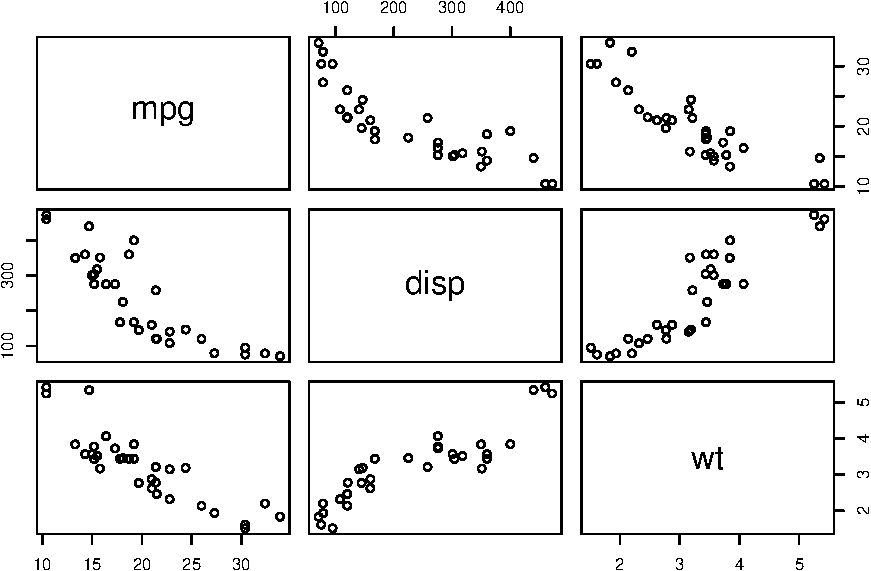
\includegraphics{05-DataMan_files/figure-latex/unnamed-chunk-26-1.pdf}

\hypertarget{merge}{%
\section{\texorpdfstring{\texttt{merge()}}{merge()}}\label{merge}}

The \texttt{merge()} function merges two data frames by common columns or row names, or do other versions of database join operations. Here is an example:

\begin{Shaded}
\begin{Highlighting}[]
\NormalTok{df1 }\OtherTok{=} \FunctionTok{data.frame}\NormalTok{(}\AttributeTok{StudentId =} \FunctionTok{c}\NormalTok{(}\DecValTok{1}\SpecialCharTok{:}\DecValTok{6}\NormalTok{), }
                 \AttributeTok{Marks =} \FunctionTok{c}\NormalTok{(}\StringTok{"70"}\NormalTok{, }\StringTok{"84"}\NormalTok{, }\StringTok{"90"}\NormalTok{, }\StringTok{"93"}\NormalTok{, }\StringTok{"80"}\NormalTok{, }\StringTok{"76"}\NormalTok{))}

\NormalTok{df2 }\OtherTok{=} \FunctionTok{data.frame}\NormalTok{(}\AttributeTok{StudentId =} \FunctionTok{c}\NormalTok{(}\DecValTok{2}\NormalTok{, }\DecValTok{4}\NormalTok{, }\DecValTok{6}\NormalTok{, }\DecValTok{7}\NormalTok{, }\DecValTok{8}\NormalTok{), }
                 \AttributeTok{city =} \FunctionTok{c}\NormalTok{(}\StringTok{"Lahore"}\NormalTok{, }\StringTok{"Karachi"}\NormalTok{, }\StringTok{"Peshawar"}\NormalTok{, }\StringTok{"Quetta"}\NormalTok{, }\StringTok{"Multan"}\NormalTok{)) }

\NormalTok{df3 }\OtherTok{=} \FunctionTok{merge}\NormalTok{(df1, df2, }\AttributeTok{by =} \StringTok{"StudentId"}\NormalTok{)}
\NormalTok{df3}
\end{Highlighting}
\end{Shaded}

\begin{verbatim}
##   StudentId Marks     city
## 1         2    84   Lahore
## 2         4    93  Karachi
## 3         6    76 Peshawar
\end{verbatim}

\begin{Shaded}
\begin{Highlighting}[]
\NormalTok{df4 }\OtherTok{=} \FunctionTok{merge}\NormalTok{(df1, df2, }\AttributeTok{by =} \StringTok{"StudentId"}\NormalTok{, }\AttributeTok{all =} \ConstantTok{TRUE}\NormalTok{)}
\NormalTok{df4}
\end{Highlighting}
\end{Shaded}

\begin{verbatim}
##   StudentId Marks     city
## 1         1    70     <NA>
## 2         2    84   Lahore
## 3         3    90     <NA>
## 4         4    93  Karachi
## 5         5    80     <NA>
## 6         6    76 Peshawar
## 7         7  <NA>   Quetta
## 8         8  <NA>   Multan
\end{verbatim}

See the options of \texttt{merge()} by \texttt{?merge}. We can do the same operation in \texttt{dplyr}:

\begin{Shaded}
\begin{Highlighting}[]
\FunctionTok{library}\NormalTok{(dplyr)}
\NormalTok{df3}\OtherTok{=}\NormalTok{ df1 }\SpecialCharTok{\%\textgreater{}\%} \FunctionTok{inner\_join}\NormalTok{(df2,}\AttributeTok{by=}\StringTok{"StudentId"}\NormalTok{)}
\NormalTok{df3}
\end{Highlighting}
\end{Shaded}

\begin{verbatim}
##   StudentId Marks     city
## 1         2    84   Lahore
## 2         4    93  Karachi
## 3         6    76 Peshawar
\end{verbatim}

\hypertarget{programing-basics}{%
\chapter{Programing basics}\label{programing-basics}}

In this section we see three main applications: conditional flows, loops, and functions, that are main pillars of any type of programming.

\hypertarget{conditional-flows}{%
\section{Conditional flows}\label{conditional-flows}}

\hypertarget{ifelse}{%
\subsection{if/else}\label{ifelse}}

The main syntax is as follows

\texttt{if\ (condition)\ \{}\strut \\
\textbf{some R code}\\
\texttt{\}\ else\ \{}\strut \\
\textbf{more R code}\\
\texttt{\}}

Here is a simple example:

\begin{Shaded}
\begin{Highlighting}[]
\NormalTok{x }\OtherTok{\textless{}{-}} \FunctionTok{c}\NormalTok{(}\StringTok{"what"}\NormalTok{,}\StringTok{"is"}\NormalTok{,}\StringTok{"truth"}\NormalTok{)}

\ControlFlowTok{if}\NormalTok{(}\StringTok{"Truth"} \SpecialCharTok{\%in\%}\NormalTok{ x) \{}
   \FunctionTok{print}\NormalTok{(}\StringTok{"Truth is found"}\NormalTok{)}
\NormalTok{\} }\ControlFlowTok{else}\NormalTok{ \{}
   \FunctionTok{print}\NormalTok{(}\StringTok{"Truth is not found"}\NormalTok{)}
\NormalTok{\}}
\end{Highlighting}
\end{Shaded}

\begin{verbatim}
## [1] "Truth is not found"
\end{verbatim}

How about this:

\begin{Shaded}
\begin{Highlighting}[]
\NormalTok{x }\OtherTok{\textless{}{-}} \FunctionTok{c}\NormalTok{(}\DecValTok{1}\NormalTok{, }\DecValTok{4}\NormalTok{, }\DecValTok{4}\NormalTok{)}
\NormalTok{a }\OtherTok{\textless{}{-}} \DecValTok{3}

\CommentTok{\#Here is a nice if/Else}
\ControlFlowTok{if}\NormalTok{(}\FunctionTok{length}\NormalTok{(x[x }\SpecialCharTok{==}\NormalTok{ a]) }\SpecialCharTok{\textgreater{}} \DecValTok{0}\NormalTok{) \{}
  \FunctionTok{print}\NormalTok{(}\FunctionTok{paste}\NormalTok{(}\StringTok{"x has"}\NormalTok{, }\FunctionTok{length}\NormalTok{(x[x}\SpecialCharTok{==}\NormalTok{a]), a))}
\NormalTok{\} }\ControlFlowTok{else}\NormalTok{ \{}
  \FunctionTok{print}\NormalTok{(}\FunctionTok{paste}\NormalTok{(}\StringTok{"x doesn\textquotesingle{}t have any"}\NormalTok{, a))}
\NormalTok{\}}
\end{Highlighting}
\end{Shaded}

\begin{verbatim}
## [1] "x doesn't have any 3"
\end{verbatim}

\begin{Shaded}
\begin{Highlighting}[]
\CommentTok{\#Another one with pipping}
\NormalTok{a }\OtherTok{\textless{}{-}} \DecValTok{4}
\ControlFlowTok{if}\NormalTok{(a }\SpecialCharTok{\%in\%}\NormalTok{ x) \{}
  \FunctionTok{print}\NormalTok{(}\FunctionTok{paste}\NormalTok{(}\StringTok{"x has"}\NormalTok{, }\FunctionTok{length}\NormalTok{(x[x}\SpecialCharTok{==}\NormalTok{a]), a))}
\NormalTok{\} }\ControlFlowTok{else}\NormalTok{ \{}
  \FunctionTok{print}\NormalTok{(}\FunctionTok{paste}\NormalTok{(}\StringTok{"x doesn\textquotesingle{}t have any"}\NormalTok{, a))}
\NormalTok{\}}
\end{Highlighting}
\end{Shaded}

\begin{verbatim}
## [1] "x has 2 4"
\end{verbatim}

\hypertarget{nested-conditions}{%
\subsection{Nested conditions}\label{nested-conditions}}

\begin{Shaded}
\begin{Highlighting}[]
\CommentTok{\#Change the numbers to see all conditions}
\NormalTok{x }\OtherTok{\textless{}{-}} \DecValTok{0}
\NormalTok{y }\OtherTok{\textless{}{-}} \DecValTok{4}
\ControlFlowTok{if}\NormalTok{ (x }\SpecialCharTok{==} \DecValTok{0} \SpecialCharTok{\&}\NormalTok{ y}\SpecialCharTok{!=} \DecValTok{0}\NormalTok{) \{}
  \FunctionTok{print}\NormalTok{(}\StringTok{"a number cannot be divided by zero"}\NormalTok{)}
\NormalTok{\} }\ControlFlowTok{else} \ControlFlowTok{if}\NormalTok{ (x }\SpecialCharTok{==} \DecValTok{0} \SpecialCharTok{\&}\NormalTok{ y }\SpecialCharTok{==} \DecValTok{0}\NormalTok{) \{}
  \FunctionTok{print}\NormalTok{(}\StringTok{"a zero cannot be divided by zero"}\NormalTok{)}
\NormalTok{\} }\ControlFlowTok{else}\NormalTok{ \{}
\NormalTok{  a }\OtherTok{\textless{}{-}}\NormalTok{ y}\SpecialCharTok{/}\NormalTok{x }
  \FunctionTok{print}\NormalTok{(}\FunctionTok{paste}\NormalTok{(}\StringTok{"y/x = "}\NormalTok{, a))}
\NormalTok{\}}
\end{Highlighting}
\end{Shaded}

\begin{verbatim}
## [1] "a number cannot be divided by zero"
\end{verbatim}

Building multiple conditions without else (it's a silly example!):

\begin{Shaded}
\begin{Highlighting}[]
\NormalTok{z }\OtherTok{\textless{}{-}} \DecValTok{0}
\NormalTok{w }\OtherTok{\textless{}{-}} \DecValTok{4}
\NormalTok{x }\OtherTok{\textless{}{-}} \DecValTok{5}
\NormalTok{y }\OtherTok{\textless{}{-}} \DecValTok{3}
\ControlFlowTok{if}\NormalTok{(z }\SpecialCharTok{\textgreater{}}\NormalTok{ w) }\FunctionTok{print}\NormalTok{(}\StringTok{"z is bigger than w"}\NormalTok{)}
\ControlFlowTok{if}\NormalTok{(w }\SpecialCharTok{\textgreater{}}\NormalTok{ z) }\FunctionTok{print}\NormalTok{(}\StringTok{"w is bigger than z"}\NormalTok{)}
\end{Highlighting}
\end{Shaded}

\begin{verbatim}
## [1] "w is bigger than z"
\end{verbatim}

\begin{Shaded}
\begin{Highlighting}[]
\ControlFlowTok{if}\NormalTok{(x }\SpecialCharTok{\textgreater{}}\NormalTok{ y) }\FunctionTok{print}\NormalTok{(}\StringTok{"x is bigger than y"}\NormalTok{)}
\end{Highlighting}
\end{Shaded}

\begin{verbatim}
## [1] "x is bigger than y"
\end{verbatim}

\begin{Shaded}
\begin{Highlighting}[]
\ControlFlowTok{if}\NormalTok{(y }\SpecialCharTok{\textgreater{}}\NormalTok{ x) }\FunctionTok{print}\NormalTok{(}\StringTok{"y is bigger than x"}\NormalTok{)}
\ControlFlowTok{if}\NormalTok{(z }\SpecialCharTok{\textgreater{}}\NormalTok{ x) }\FunctionTok{print}\NormalTok{(}\StringTok{"z is bigger than x"}\NormalTok{)}
\ControlFlowTok{if}\NormalTok{(x }\SpecialCharTok{\textgreater{}}\NormalTok{ z) }\FunctionTok{print}\NormalTok{(}\StringTok{"x is bigger than z"}\NormalTok{)}
\end{Highlighting}
\end{Shaded}

\begin{verbatim}
## [1] "x is bigger than z"
\end{verbatim}

\begin{Shaded}
\begin{Highlighting}[]
\ControlFlowTok{if}\NormalTok{(w }\SpecialCharTok{\textgreater{}}\NormalTok{ y) }\FunctionTok{print}\NormalTok{(}\StringTok{"w is bigger than y"}\NormalTok{)}
\end{Highlighting}
\end{Shaded}

\begin{verbatim}
## [1] "w is bigger than y"
\end{verbatim}

\begin{Shaded}
\begin{Highlighting}[]
\ControlFlowTok{if}\NormalTok{(y }\SpecialCharTok{\textgreater{}}\NormalTok{ w) }\FunctionTok{print}\NormalTok{(}\StringTok{"y is bigger than w"}\NormalTok{)}
\end{Highlighting}
\end{Shaded}

\hypertarget{simpler-ifelse}{%
\subsection{\texorpdfstring{Simpler \texttt{ifelse}}{Simpler ifelse}}\label{simpler-ifelse}}

A simpler, one-line \texttt{ifelse}:

\begin{Shaded}
\begin{Highlighting}[]
\CommentTok{\#Change the numbers}
\NormalTok{x }\OtherTok{\textless{}{-}} \DecValTok{0}
\NormalTok{y }\OtherTok{\textless{}{-}} \DecValTok{4}
\FunctionTok{ifelse}\NormalTok{ (x }\SpecialCharTok{\textgreater{}}\NormalTok{ y, }\StringTok{"x is bigger than y"}\NormalTok{, }\StringTok{"y is bigger than x"}\NormalTok{)}
\end{Highlighting}
\end{Shaded}

\begin{verbatim}
## [1] "y is bigger than x"
\end{verbatim}

\begin{Shaded}
\begin{Highlighting}[]
\CommentTok{\#Better (ifelse will fail if x = y.  Try it!)}
\FunctionTok{ifelse}\NormalTok{ (x }\SpecialCharTok{==}\NormalTok{ y, }\StringTok{"x is the same as y"}\NormalTok{,}
        \FunctionTok{ifelse}\NormalTok{(x }\SpecialCharTok{\textgreater{}}\NormalTok{ y, }\StringTok{"x is bigger than y"}\NormalTok{, }\StringTok{"y is bigger than x"}\NormalTok{))}
\end{Highlighting}
\end{Shaded}

\begin{verbatim}
## [1] "y is bigger than x"
\end{verbatim}

A simpler, without else!

\begin{Shaded}
\begin{Highlighting}[]
\NormalTok{z }\OtherTok{\textless{}{-}} \DecValTok{0}
\NormalTok{w }\OtherTok{\textless{}{-}} \DecValTok{4}
\ControlFlowTok{if}\NormalTok{(z }\SpecialCharTok{\textgreater{}}\NormalTok{ w) }\FunctionTok{print}\NormalTok{(}\StringTok{"w is bigger than z"}\NormalTok{)}

\CommentTok{\#Change the numbers}
\NormalTok{x }\OtherTok{\textless{}{-}} \DecValTok{5}
\NormalTok{y }\OtherTok{\textless{}{-}} \DecValTok{3}
\ControlFlowTok{if}\NormalTok{(x }\SpecialCharTok{\textgreater{}}\NormalTok{ y) }\FunctionTok{print}\NormalTok{(}\StringTok{"x is bigger than y"}\NormalTok{)}
\end{Highlighting}
\end{Shaded}

\begin{verbatim}
## [1] "x is bigger than y"
\end{verbatim}

\begin{Shaded}
\begin{Highlighting}[]
\CommentTok{\#See that both of them moves to the next line.}
\end{Highlighting}
\end{Shaded}

The \texttt{ifelse()} function only allows for one ``if'' statement, two cases. You could add nested ``if'' statements, but that's just a pain, especially if the 3+ conditions you want to use are all on the same level, conceptually. Is there a way to specify multiple conditions at the same time?

\begin{Shaded}
\begin{Highlighting}[]
\CommentTok{\#Let\textquotesingle{}s create a data frame:}
\NormalTok{df }\OtherTok{\textless{}{-}} \FunctionTok{data.frame}\NormalTok{(}\StringTok{"name"}\OtherTok{=}\FunctionTok{c}\NormalTok{(}\StringTok{"Kaija"}\NormalTok{, }\StringTok{"Ella"}\NormalTok{, }\StringTok{"Andis"}\NormalTok{), }\StringTok{"test1"} \OtherTok{=} \FunctionTok{c}\NormalTok{(}\ConstantTok{FALSE}\NormalTok{, }\ConstantTok{TRUE}\NormalTok{, }\ConstantTok{TRUE}\NormalTok{),}
                 \StringTok{"test2"} \OtherTok{=} \FunctionTok{c}\NormalTok{(}\ConstantTok{FALSE}\NormalTok{, }\ConstantTok{FALSE}\NormalTok{, }\ConstantTok{TRUE}\NormalTok{))}
\NormalTok{df}
\end{Highlighting}
\end{Shaded}

\begin{verbatim}
##    name test1 test2
## 1 Kaija FALSE FALSE
## 2  Ella  TRUE FALSE
## 3 Andis  TRUE  TRUE
\end{verbatim}

Suppose we want separate the people into three groups:

\begin{itemize}
\tightlist
\item
  People who passed both tests: Group A\\
\item
  People who passed one test: Group B
\item
  People who passed neither test: Group C
\end{itemize}

\texttt{dplyr} has a function for exactly this purpose: \texttt{case\_when()}.

\begin{Shaded}
\begin{Highlighting}[]
\FunctionTok{library}\NormalTok{(dplyr)}
\NormalTok{df }\OtherTok{\textless{}{-}}\NormalTok{ df }\SpecialCharTok{\%\textgreater{}\%} 
\FunctionTok{mutate}\NormalTok{(}\AttributeTok{group =} \FunctionTok{case\_when}\NormalTok{(test1 }\SpecialCharTok{\&}\NormalTok{ test2 }\SpecialCharTok{\textasciitilde{}} \StringTok{"A"}\NormalTok{, }\CommentTok{\# both tests: group A}
                         \FunctionTok{xor}\NormalTok{(test1, test2) }\SpecialCharTok{\textasciitilde{}} \StringTok{"B"}\NormalTok{, }\CommentTok{\# one test: group B}
                         \SpecialCharTok{!}\NormalTok{test1 }\SpecialCharTok{\&} \SpecialCharTok{!}\NormalTok{test2 }\SpecialCharTok{\textasciitilde{}} \StringTok{"C"} \CommentTok{\# neither test: group C}
\NormalTok{))}
\NormalTok{df}
\end{Highlighting}
\end{Shaded}

\begin{verbatim}
##    name test1 test2 group
## 1 Kaija FALSE FALSE     C
## 2  Ella  TRUE FALSE     B
## 3 Andis  TRUE  TRUE     A
\end{verbatim}

\hypertarget{loops}{%
\section{Loops}\label{loops}}

What would you do if you needed to execute a block of code multiple times? In general, statements are executed sequentially. A loop statement allows us to execute a statement or group of statements multiple times and the following is the general form of a loop statement in most programming languages. There are 3 main loop types: \texttt{while()}, \texttt{for()}, \texttt{repeat()}.

Here are some examples for \texttt{for()} loop:

\begin{Shaded}
\begin{Highlighting}[]
\NormalTok{x }\OtherTok{\textless{}{-}} \FunctionTok{c}\NormalTok{(}\DecValTok{3}\NormalTok{, }\SpecialCharTok{{-}}\DecValTok{1}\NormalTok{, }\DecValTok{4}\NormalTok{, }\DecValTok{2}\NormalTok{, }\DecValTok{10}\NormalTok{, }\DecValTok{5}\NormalTok{)}

\ControlFlowTok{for}\NormalTok{ (i }\ControlFlowTok{in} \DecValTok{1}\SpecialCharTok{:}\FunctionTok{length}\NormalTok{(x)) \{}
\NormalTok{  x[i] }\OtherTok{\textless{}{-}}\NormalTok{ x[i] }\SpecialCharTok{*} \DecValTok{2}
\NormalTok{\}}

\NormalTok{x}
\end{Highlighting}
\end{Shaded}

\begin{verbatim}
## [1]  6 -2  8  4 20 10
\end{verbatim}

Note that this just for an example. If we want to multiply each element of a vector by 2, a loop isn't the best way. Although it is very normal in many programming languages, we would simply use a vectorized operation in R.

\begin{Shaded}
\begin{Highlighting}[]
\NormalTok{x }\OtherTok{\textless{}{-}} \FunctionTok{c}\NormalTok{(}\DecValTok{3}\NormalTok{, }\SpecialCharTok{{-}}\DecValTok{1}\NormalTok{, }\DecValTok{4}\NormalTok{, }\DecValTok{2}\NormalTok{, }\DecValTok{10}\NormalTok{, }\DecValTok{5}\NormalTok{)}
\NormalTok{x }\OtherTok{\textless{}{-}}\NormalTok{ x }\SpecialCharTok{*} \DecValTok{2}
\NormalTok{x}
\end{Highlighting}
\end{Shaded}

\begin{verbatim}
## [1]  6 -2  8  4 20 10
\end{verbatim}

\hypertarget{conditional-loops}{%
\subsection{Conditional loops}\label{conditional-loops}}

But some times it would be very handy. If the element in \(x > 3\), multiply it with the subsequent element:

\begin{Shaded}
\begin{Highlighting}[]
\NormalTok{x }\OtherTok{\textless{}{-}} \FunctionTok{c}\NormalTok{(}\DecValTok{3}\NormalTok{, }\SpecialCharTok{{-}}\DecValTok{1}\NormalTok{, }\DecValTok{0}\NormalTok{, }\DecValTok{2}\NormalTok{, }\DecValTok{10}\NormalTok{, }\DecValTok{5}\NormalTok{)}

\NormalTok{x\_new }\OtherTok{\textless{}{-}} \FunctionTok{c}\NormalTok{() }\CommentTok{\#empty container}
\ControlFlowTok{for}\NormalTok{ (i }\ControlFlowTok{in} \DecValTok{1}\SpecialCharTok{:}\NormalTok{(}\FunctionTok{length}\NormalTok{(x)}\SpecialCharTok{{-}}\DecValTok{1}\NormalTok{)) \{}
  \FunctionTok{ifelse}\NormalTok{(x[i] }\SpecialCharTok{\textgreater{}} \DecValTok{3}\NormalTok{,  x\_new[i] }\OtherTok{\textless{}{-}}\NormalTok{ x[i] }\SpecialCharTok{*}\NormalTok{ x[i }\SpecialCharTok{+} \DecValTok{1}\NormalTok{], x\_new[i] }\OtherTok{\textless{}{-}} \DecValTok{0}\NormalTok{)  }
\NormalTok{\}}

\NormalTok{x}
\end{Highlighting}
\end{Shaded}

\begin{verbatim}
## [1]  3 -1  0  2 10  5
\end{verbatim}

\begin{Shaded}
\begin{Highlighting}[]
\NormalTok{x\_new}
\end{Highlighting}
\end{Shaded}

\begin{verbatim}
## [1]  0  0  0  0 50
\end{verbatim}

Inside the \texttt{if} and \texttt{else} clause, you can use \texttt{next} and \texttt{break} to further control the flow. The \texttt{next} function goes directly to the next loop cycle, while \texttt{break} jumped out of the current loop.

\begin{Shaded}
\begin{Highlighting}[]
\NormalTok{x }\OtherTok{\textless{}{-}} \FunctionTok{c}\NormalTok{(}\DecValTok{9}\NormalTok{, }\SpecialCharTok{{-}}\DecValTok{1}\NormalTok{, }\DecValTok{0}\NormalTok{, }\DecValTok{5}\NormalTok{, }\SpecialCharTok{{-}}\DecValTok{7}\NormalTok{, }\DecValTok{16}\NormalTok{, }\DecValTok{22}\NormalTok{)}
\NormalTok{zn }\OtherTok{\textless{}{-}} \FunctionTok{c}\NormalTok{()}

\ControlFlowTok{for}\NormalTok{(i }\ControlFlowTok{in} \DecValTok{1}\SpecialCharTok{:}\FunctionTok{length}\NormalTok{(x))\{ }
  \ControlFlowTok{if}\NormalTok{(x[i] }\SpecialCharTok{\textless{}} \DecValTok{0}\NormalTok{)\{ }
    \ControlFlowTok{next}
\NormalTok{  \} }
\NormalTok{  zn }\OtherTok{\textless{}{-}} \FunctionTok{c}\NormalTok{(zn,  }\FunctionTok{sqrt}\NormalTok{(x[i]))}
\NormalTok{\}}

\NormalTok{zn}
\end{Highlighting}
\end{Shaded}

\begin{verbatim}
## [1] 3.000000 0.000000 2.236068 4.000000 4.690416
\end{verbatim}

Inside the \texttt{if} and \texttt{else} clause, you can use \texttt{next} and \texttt{break} to further control the flow. The \texttt{next} function goes directly to the next loop cycle, while \texttt{break} jumped out of the current loop.

\begin{Shaded}
\begin{Highlighting}[]
\NormalTok{x }\OtherTok{\textless{}{-}} \FunctionTok{c}\NormalTok{(}\DecValTok{9}\NormalTok{, }\DecValTok{1}\NormalTok{, }\DecValTok{0}\NormalTok{, }\DecValTok{5}\NormalTok{, }\DecValTok{7}\NormalTok{, }\DecValTok{16}\NormalTok{, }\DecValTok{22}\NormalTok{)}
\NormalTok{bn }\OtherTok{\textless{}{-}} \FunctionTok{c}\NormalTok{()}

\ControlFlowTok{for}\NormalTok{(i }\ControlFlowTok{in} \DecValTok{1}\SpecialCharTok{:}\FunctionTok{length}\NormalTok{(x))\{ }
  \ControlFlowTok{if}\NormalTok{(x[i] }\SpecialCharTok{\textgreater{}} \DecValTok{10}\NormalTok{)\{ }
    \ControlFlowTok{break}
\NormalTok{  \} }
\NormalTok{  bn }\OtherTok{\textless{}{-}} \FunctionTok{c}\NormalTok{(bn,  }\FunctionTok{sqrt}\NormalTok{(x[i]))}
\NormalTok{\}}

\NormalTok{bn}
\end{Highlighting}
\end{Shaded}

\begin{verbatim}
## [1] 3.000000 1.000000 0.000000 2.236068 2.645751
\end{verbatim}

\hypertarget{while-and-repeat}{%
\subsection{\texorpdfstring{\texttt{while()} and \texttt{repeat()}}{while() and repeat()}}\label{while-and-repeat}}

Here are some examples for \texttt{while()} loop:

\begin{Shaded}
\begin{Highlighting}[]
\CommentTok{\# Let\textquotesingle{}s use our first example}

\NormalTok{x }\OtherTok{\textless{}{-}} \DecValTok{3}
\NormalTok{cnt }\OtherTok{\textless{}{-}} \DecValTok{1}

\ControlFlowTok{while}\NormalTok{ (cnt }\SpecialCharTok{\textless{}} \DecValTok{11}\NormalTok{) \{}
\NormalTok{   x }\OtherTok{=}\NormalTok{ x }\SpecialCharTok{*} \DecValTok{2}
\NormalTok{   cnt }\OtherTok{=}\NormalTok{ cnt }\SpecialCharTok{+} \DecValTok{1}
\NormalTok{\}}
\NormalTok{x}
\end{Highlighting}
\end{Shaded}

\begin{verbatim}
## [1] 3072
\end{verbatim}

Here are some examples for \texttt{repeat()} loop:

\begin{Shaded}
\begin{Highlighting}[]
\CommentTok{\# Let\textquotesingle{}s use our first example}

\NormalTok{x }\OtherTok{\textless{}{-}} \DecValTok{3}
\NormalTok{cnt }\OtherTok{\textless{}{-}} \DecValTok{1}

\ControlFlowTok{repeat}\NormalTok{ \{}
\NormalTok{   x }\OtherTok{=}\NormalTok{ x }\SpecialCharTok{*} \DecValTok{2}
\NormalTok{   cnt }\OtherTok{=}\NormalTok{ cnt }\SpecialCharTok{+} \DecValTok{1}
  
   \ControlFlowTok{if}\NormalTok{(cnt }\SpecialCharTok{\textgreater{}} \DecValTok{10}\NormalTok{) }\ControlFlowTok{break}
\NormalTok{\}}
\NormalTok{x}
\end{Highlighting}
\end{Shaded}

\begin{verbatim}
## [1] 3072
\end{verbatim}

\hypertarget{nested-loops}{%
\subsection{Nested loops}\label{nested-loops}}

It is also common to put one loop inside another one. Let's say we want to create a 5x5 matrix where each element \(A_{i j}=i+j\)

\begin{Shaded}
\begin{Highlighting}[]
\NormalTok{A }\OtherTok{\textless{}{-}} \FunctionTok{matrix}\NormalTok{(}\DecValTok{0}\NormalTok{, }\DecValTok{5}\NormalTok{, }\DecValTok{5}\NormalTok{) }\CommentTok{\#initialize the matrix A}

\ControlFlowTok{for}\NormalTok{ (i }\ControlFlowTok{in} \DecValTok{1}\SpecialCharTok{:}\DecValTok{5}\NormalTok{)       }\CommentTok{\#loop over index i}
  \ControlFlowTok{for}\NormalTok{ (j }\ControlFlowTok{in} \DecValTok{1}\SpecialCharTok{:}\DecValTok{5}\NormalTok{)\{    }\CommentTok{\#loop over index j}
\NormalTok{    A[i, j] }\OtherTok{\textless{}{-}}\NormalTok{ i }\SpecialCharTok{+}\NormalTok{ j }\CommentTok{\#set the (i, j){-}th element of A}
\NormalTok{  \}}
\NormalTok{A}
\end{Highlighting}
\end{Shaded}

\begin{verbatim}
##      [,1] [,2] [,3] [,4] [,5]
## [1,]    2    3    4    5    6
## [2,]    3    4    5    6    7
## [3,]    4    5    6    7    8
## [4,]    5    6    7    8    9
## [5,]    6    7    8    9   10
\end{verbatim}

\hypertarget{outer}{%
\subsection{\texorpdfstring{\texttt{outer()}}{outer()}}\label{outer}}

\texttt{outer()} takes two vectors and a function (that itself takes two arguments) and builds a \textbf{matrix} by calling the given function for each combination of the elements in the two vectors.

\begin{Shaded}
\begin{Highlighting}[]
\NormalTok{x }\OtherTok{\textless{}{-}} \FunctionTok{c}\NormalTok{(}\DecValTok{0}\NormalTok{, }\DecValTok{1}\NormalTok{, }\DecValTok{2}\NormalTok{)}
\NormalTok{y }\OtherTok{\textless{}{-}} \FunctionTok{c}\NormalTok{(}\DecValTok{0}\NormalTok{, }\DecValTok{1}\NormalTok{, }\DecValTok{2}\NormalTok{, }\DecValTok{3}\NormalTok{, }\DecValTok{4}\NormalTok{)}

\NormalTok{m }\OtherTok{\textless{}{-}} \FunctionTok{outer}\NormalTok{ (}
\NormalTok{   y,     }\CommentTok{\# First dimension:  the columns (y)}
\NormalTok{   x,     }\CommentTok{\# Second dimension: the rows    (x)}
   \ControlFlowTok{function}\NormalTok{ (x, y)   x}\SpecialCharTok{+}\DecValTok{2}\SpecialCharTok{*}\NormalTok{y}
\NormalTok{)}

\NormalTok{m}
\end{Highlighting}
\end{Shaded}

\begin{verbatim}
##      [,1] [,2] [,3]
## [1,]    0    2    4
## [2,]    1    3    5
## [3,]    2    4    6
## [4,]    3    5    7
## [5,]    4    6    8
\end{verbatim}

In place of the function, an operator can be given, which makes it easy to create a matrix with simple calculations (such as multiplying):

\begin{Shaded}
\begin{Highlighting}[]
\NormalTok{m }\OtherTok{\textless{}{-}} \FunctionTok{outer}\NormalTok{(}\FunctionTok{c}\NormalTok{(}\DecValTok{10}\NormalTok{, }\DecValTok{20}\NormalTok{, }\DecValTok{30}\NormalTok{, }\DecValTok{40}\NormalTok{), }\FunctionTok{c}\NormalTok{(}\DecValTok{2}\NormalTok{, }\DecValTok{4}\NormalTok{, }\DecValTok{6}\NormalTok{), }\StringTok{"*"}\NormalTok{)}
\NormalTok{m}
\end{Highlighting}
\end{Shaded}

\begin{verbatim}
##      [,1] [,2] [,3]
## [1,]   20   40   60
## [2,]   40   80  120
## [3,]   60  120  180
## [4,]   80  160  240
\end{verbatim}

It becomes very handy when we build a polynomial model:

\begin{Shaded}
\begin{Highlighting}[]
\NormalTok{x }\OtherTok{\textless{}{-}} \FunctionTok{sample}\NormalTok{(}\DecValTok{0}\SpecialCharTok{:}\DecValTok{20}\NormalTok{, }\DecValTok{10}\NormalTok{, }\AttributeTok{replace =} \ConstantTok{TRUE}\NormalTok{)}
\NormalTok{x}
\end{Highlighting}
\end{Shaded}

\begin{verbatim}
##  [1]  7  9 19 10  0  5 17 10  7  9
\end{verbatim}

\begin{Shaded}
\begin{Highlighting}[]
\NormalTok{m }\OtherTok{\textless{}{-}} \FunctionTok{outer}\NormalTok{(x, }\DecValTok{1}\SpecialCharTok{:}\DecValTok{4}\NormalTok{, }\StringTok{"\^{}"}\NormalTok{)}
\NormalTok{m}
\end{Highlighting}
\end{Shaded}

\begin{verbatim}
##       [,1] [,2] [,3]   [,4]
##  [1,]    7   49  343   2401
##  [2,]    9   81  729   6561
##  [3,]   19  361 6859 130321
##  [4,]   10  100 1000  10000
##  [5,]    0    0    0      0
##  [6,]    5   25  125    625
##  [7,]   17  289 4913  83521
##  [8,]   10  100 1000  10000
##  [9,]    7   49  343   2401
## [10,]    9   81  729   6561
\end{verbatim}

We can also use \texttt{outer()} for this example

\begin{Shaded}
\begin{Highlighting}[]
\FunctionTok{outer}\NormalTok{(}\DecValTok{1}\SpecialCharTok{:}\DecValTok{5}\NormalTok{, }\DecValTok{1}\SpecialCharTok{:}\DecValTok{5}\NormalTok{, }\StringTok{"+"}\NormalTok{)}
\end{Highlighting}
\end{Shaded}

\begin{verbatim}
##      [,1] [,2] [,3] [,4] [,5]
## [1,]    2    3    4    5    6
## [2,]    3    4    5    6    7
## [3,]    4    5    6    7    8
## [4,]    5    6    7    8    9
## [5,]    6    7    8    9   10
\end{verbatim}

\begin{Shaded}
\begin{Highlighting}[]
\CommentTok{\# Or}

\FunctionTok{outer}\NormalTok{(}\DecValTok{1}\SpecialCharTok{:}\DecValTok{4}\NormalTok{, }\DecValTok{1}\SpecialCharTok{:}\DecValTok{4}\NormalTok{, }\ControlFlowTok{function}\NormalTok{(i, j)\{}\FloatTok{0.5}\SpecialCharTok{\^{}}\NormalTok{\{}\FunctionTok{abs}\NormalTok{(i}\SpecialCharTok{{-}}\NormalTok{j)\}\})}
\end{Highlighting}
\end{Shaded}

\begin{verbatim}
##       [,1] [,2] [,3]  [,4]
## [1,] 1.000 0.50 0.25 0.125
## [2,] 0.500 1.00 0.50 0.250
## [3,] 0.250 0.50 1.00 0.500
## [4,] 0.125 0.25 0.50 1.000
\end{verbatim}

\hypertarget{the-apply-family}{%
\section{\texorpdfstring{The \texttt{apply()} family}{The apply() family}}\label{the-apply-family}}

The \texttt{apply()} family is one of the R base packages and is populated with functions to manipulate slices of data from matrices, arrays, lists and data frames in a repetitive way. These functions allow crossing the data in a number of ways and avoid explicit use of loop constructs. They act on an input list, matrix or array and apply a named function with one or several optional arguments. The family is made up of the \texttt{apply()}, \texttt{lapply()} , \texttt{sapply()}, \texttt{vapply()}, \texttt{mapply()}, \texttt{rapply()}, and \texttt{tapply()} functions.

\hypertarget{apply}{%
\subsection{\texorpdfstring{\texttt{apply()}}{apply()}}\label{apply}}

The R base manual tells you that it's called as follows: \texttt{apply(X,\ MARGIN,\ FUN,\ ...)}, where, X is an array or a matrix if the dimension of the array is 2; MARGIN is a variable defining how the function is applied: when \texttt{MARGIN=1}, it applies over rows, whereas with \texttt{MARGIN=2}, it works over columns. Note that when you use the construct \texttt{MARGIN=c(1,2)}, it applies to both rows and columns; and FUN, which is the function that you want to apply to the data. It can be any R function, including a User Defined Function (UDF).

\begin{Shaded}
\begin{Highlighting}[]
\CommentTok{\# Construct a 5x6 matrix}
\NormalTok{X }\OtherTok{\textless{}{-}} \FunctionTok{matrix}\NormalTok{(}\FunctionTok{rnorm}\NormalTok{(}\DecValTok{30}\NormalTok{), }\AttributeTok{nrow=}\DecValTok{5}\NormalTok{, }\AttributeTok{ncol=}\DecValTok{6}\NormalTok{)}

\CommentTok{\# Sum the values of each column with \textasciigrave{}apply()\textasciigrave{}}
\FunctionTok{apply}\NormalTok{(X, }\DecValTok{2}\NormalTok{, sum)}
\end{Highlighting}
\end{Shaded}

\begin{verbatim}
## [1]  2.3823217 -1.2894225 -2.4129301 -0.2844947 -1.6296557 -4.8437539
\end{verbatim}

\begin{Shaded}
\begin{Highlighting}[]
\FunctionTok{apply}\NormalTok{(X, }\DecValTok{2}\NormalTok{, length)}
\end{Highlighting}
\end{Shaded}

\begin{verbatim}
## [1] 5 5 5 5 5 5
\end{verbatim}

\begin{Shaded}
\begin{Highlighting}[]
\FunctionTok{apply}\NormalTok{(X, }\DecValTok{1}\NormalTok{, length)}
\end{Highlighting}
\end{Shaded}

\begin{verbatim}
## [1] 6 6 6 6 6
\end{verbatim}

\begin{Shaded}
\begin{Highlighting}[]
\FunctionTok{apply}\NormalTok{(X, }\DecValTok{2}\NormalTok{, }\ControlFlowTok{function}\NormalTok{ (x) }\FunctionTok{length}\NormalTok{(x)}\SpecialCharTok{{-}}\DecValTok{1}\NormalTok{)}
\end{Highlighting}
\end{Shaded}

\begin{verbatim}
## [1] 4 4 4 4 4 4
\end{verbatim}

\begin{Shaded}
\begin{Highlighting}[]
\CommentTok{\#If you don’t want to write a function inside of the arguments}
\NormalTok{len }\OtherTok{\textless{}{-}} \ControlFlowTok{function}\NormalTok{(x)\{}
  \FunctionTok{length}\NormalTok{(x)}\SpecialCharTok{{-}}\DecValTok{1}
\NormalTok{\}}
\FunctionTok{apply}\NormalTok{(X,}\DecValTok{2}\NormalTok{, len)}
\end{Highlighting}
\end{Shaded}

\begin{verbatim}
## [1] 4 4 4 4 4 4
\end{verbatim}

\begin{Shaded}
\begin{Highlighting}[]
\CommentTok{\#It can also be used to repeat a function on cells within a matrix}
\NormalTok{X\_new }\OtherTok{\textless{}{-}} \FunctionTok{apply}\NormalTok{(X[}\DecValTok{1}\SpecialCharTok{:}\DecValTok{2}\NormalTok{,], }\DecValTok{1}\NormalTok{, }\ControlFlowTok{function}\NormalTok{(x) x}\SpecialCharTok{+}\DecValTok{1}\NormalTok{)}
\NormalTok{X\_new}
\end{Highlighting}
\end{Shaded}

\begin{verbatim}
##              [,1]         [,2]
## [1,]  1.448670734  1.788860514
## [2,]  1.750915324  0.722027088
## [3,]  0.833623757  0.949493235
## [4,]  0.001116069  0.738579066
## [5,]  1.769290662  1.783511818
## [6,] -0.044204172 -0.006294795
\end{verbatim}

Since \texttt{apply()} is used only for matrices, if you apply \texttt{apply()} to a data frame, it first coerces your data.frame to an array which means all the columns must have the same type. Depending on your context, this could have unintended consequences. For a safer practice in data frames, we can use \texttt{lappy()} and \texttt{sapply()}:

\hypertarget{lapply}{%
\subsection{\texorpdfstring{\texttt{lapply()}}{lapply()}}\label{lapply}}

You want to apply a given function to every element of a list and obtain a list as a result. When you execute \texttt{?lapply}, you see that the syntax looks like the \texttt{apply()} function. The difference is that it can be used for other objects like data frames, lists or vectors. And the output returned is a list (which explains the ``l'' in the function name), which has the same number of elements as the object passed to it. \texttt{lapply()} function does not need MARGIN.

\begin{Shaded}
\begin{Highlighting}[]
\NormalTok{A}\OtherTok{\textless{}{-}}\FunctionTok{c}\NormalTok{(}\DecValTok{1}\SpecialCharTok{:}\DecValTok{9}\NormalTok{)}
\NormalTok{B}\OtherTok{\textless{}{-}}\FunctionTok{c}\NormalTok{(}\DecValTok{1}\SpecialCharTok{:}\DecValTok{12}\NormalTok{)}
\NormalTok{C}\OtherTok{\textless{}{-}}\FunctionTok{c}\NormalTok{(}\DecValTok{1}\SpecialCharTok{:}\DecValTok{15}\NormalTok{)}
\NormalTok{my.lst}\OtherTok{\textless{}{-}}\FunctionTok{list}\NormalTok{(A,B,C)}
\FunctionTok{lapply}\NormalTok{(my.lst, sum)}
\end{Highlighting}
\end{Shaded}

\begin{verbatim}
## [[1]]
## [1] 45
## 
## [[2]]
## [1] 78
## 
## [[3]]
## [1] 120
\end{verbatim}

\hypertarget{sapply}{%
\subsection{\texorpdfstring{\texttt{sapply()}}{sapply()}}\label{sapply}}

\texttt{sapply} works just like \texttt{lapply}, but will simplify the output if possible. This means that instead of returning a list like \texttt{lapply}, it will return a vector instead if the data is simplifiable.

\begin{Shaded}
\begin{Highlighting}[]
\NormalTok{A}\OtherTok{\textless{}{-}}\FunctionTok{c}\NormalTok{(}\DecValTok{1}\SpecialCharTok{:}\DecValTok{9}\NormalTok{)}
\NormalTok{B}\OtherTok{\textless{}{-}}\FunctionTok{c}\NormalTok{(}\DecValTok{1}\SpecialCharTok{:}\DecValTok{12}\NormalTok{)}
\NormalTok{C}\OtherTok{\textless{}{-}}\FunctionTok{c}\NormalTok{(}\DecValTok{1}\SpecialCharTok{:}\DecValTok{15}\NormalTok{)}
\NormalTok{my.lst}\OtherTok{\textless{}{-}}\FunctionTok{list}\NormalTok{(A,B,C)}
\FunctionTok{sapply}\NormalTok{(my.lst, sum)}
\end{Highlighting}
\end{Shaded}

\begin{verbatim}
## [1]  45  78 120
\end{verbatim}

\hypertarget{tapply}{%
\subsection{\texorpdfstring{\texttt{tapply()}}{tapply()}}\label{tapply}}

Sometimes you may want to perform the apply function on some data, but have it separated by factor. In that case, you should use \texttt{tapply}. Let's take a look at the information for \texttt{tapply}.

\begin{Shaded}
\begin{Highlighting}[]
\NormalTok{X }\OtherTok{\textless{}{-}} \FunctionTok{matrix}\NormalTok{(}\FunctionTok{c}\NormalTok{(}\DecValTok{1}\SpecialCharTok{:}\DecValTok{10}\NormalTok{, }\DecValTok{11}\SpecialCharTok{:}\DecValTok{20}\NormalTok{, }\DecValTok{21}\SpecialCharTok{:}\DecValTok{30}\NormalTok{), }\AttributeTok{nrow =} \DecValTok{10}\NormalTok{, }\AttributeTok{ncol =} \DecValTok{3}\NormalTok{)}
\NormalTok{tdata }\OtherTok{\textless{}{-}} \FunctionTok{as.data.frame}\NormalTok{(}\FunctionTok{cbind}\NormalTok{(}\FunctionTok{c}\NormalTok{(}\DecValTok{1}\NormalTok{,}\DecValTok{1}\NormalTok{,}\DecValTok{1}\NormalTok{,}\DecValTok{1}\NormalTok{,}\DecValTok{1}\NormalTok{,}\DecValTok{2}\NormalTok{,}\DecValTok{2}\NormalTok{,}\DecValTok{2}\NormalTok{,}\DecValTok{2}\NormalTok{,}\DecValTok{2}\NormalTok{), X))}
\NormalTok{tdata}
\end{Highlighting}
\end{Shaded}

\begin{verbatim}
##    V1 V2 V3 V4
## 1   1  1 11 21
## 2   1  2 12 22
## 3   1  3 13 23
## 4   1  4 14 24
## 5   1  5 15 25
## 6   2  6 16 26
## 7   2  7 17 27
## 8   2  8 18 28
## 9   2  9 19 29
## 10  2 10 20 30
\end{verbatim}

\begin{Shaded}
\begin{Highlighting}[]
\FunctionTok{tapply}\NormalTok{(tdata}\SpecialCharTok{$}\NormalTok{V2, tdata}\SpecialCharTok{$}\NormalTok{V1, mean)}
\end{Highlighting}
\end{Shaded}

\begin{verbatim}
## 1 2 
## 3 8
\end{verbatim}

What we have here is an important tool: We have a conditional mean of column 2 (V2) with respect to column 1 (V1). You can use \texttt{tapply} to do some quick summary statistics on a variable split by condition.

\begin{Shaded}
\begin{Highlighting}[]
\NormalTok{summary }\OtherTok{\textless{}{-}} \FunctionTok{tapply}\NormalTok{(tdata}\SpecialCharTok{$}\NormalTok{V2, tdata}\SpecialCharTok{$}\NormalTok{V1, }\ControlFlowTok{function}\NormalTok{(x) }\FunctionTok{c}\NormalTok{(}\FunctionTok{mean}\NormalTok{(x), }\FunctionTok{sd}\NormalTok{(x)))}
\NormalTok{summary}
\end{Highlighting}
\end{Shaded}

\begin{verbatim}
## $`1`
## [1] 3.000000 1.581139
## 
## $`2`
## [1] 8.000000 1.581139
\end{verbatim}

\hypertarget{mapply}{%
\subsection{\texorpdfstring{\texttt{mapply()}}{mapply()}}\label{mapply}}

\texttt{mapply()} would be used to create a new variable. For example, using dataset \texttt{tdata}, we could divide one column by another column to create a new value. This would be useful for creating a ratio of two variables as shown in the example below.

\begin{Shaded}
\begin{Highlighting}[]
\NormalTok{tdata}\SpecialCharTok{$}\NormalTok{V5 }\OtherTok{\textless{}{-}} \FunctionTok{mapply}\NormalTok{(}\ControlFlowTok{function}\NormalTok{(x, y) x}\SpecialCharTok{/}\NormalTok{y, tdata}\SpecialCharTok{$}\NormalTok{V2, tdata}\SpecialCharTok{$}\NormalTok{V4)}
\NormalTok{tdata}\SpecialCharTok{$}\NormalTok{V5}
\end{Highlighting}
\end{Shaded}

\begin{verbatim}
##  [1] 0.04761905 0.09090909 0.13043478 0.16666667 0.20000000 0.23076923
##  [7] 0.25925926 0.28571429 0.31034483 0.33333333
\end{verbatim}

\hypertarget{functions}{%
\section{Functions}\label{functions}}

An R function is created by using the keyword function. Let's write our first function:

\begin{Shaded}
\begin{Highlighting}[]
\NormalTok{first }\OtherTok{\textless{}{-}} \ControlFlowTok{function}\NormalTok{(a)\{}
\NormalTok{  b }\OtherTok{\textless{}{-}}\NormalTok{ a }\SpecialCharTok{\^{}} \DecValTok{2}
  \FunctionTok{return}\NormalTok{(b)}
\NormalTok{\}}

\FunctionTok{first}\NormalTok{(}\DecValTok{1675}\NormalTok{)}
\end{Highlighting}
\end{Shaded}

\begin{verbatim}
## [1] 2805625
\end{verbatim}

Let's have a function that find the z-score (standardization). That's subtracting the sample mean, and dividing by the sample standard deviation.

\[
\frac{x-\overline{x}}{s}
\]

\begin{Shaded}
\begin{Highlighting}[]
\NormalTok{z\_score }\OtherTok{\textless{}{-}} \ControlFlowTok{function}\NormalTok{(x)\{}
  \FunctionTok{return}\NormalTok{((x }\SpecialCharTok{{-}} \FunctionTok{mean}\NormalTok{(x))}\SpecialCharTok{/}\FunctionTok{sd}\NormalTok{(x))}
\NormalTok{\}}

\FunctionTok{set.seed}\NormalTok{(}\DecValTok{1}\NormalTok{)}
\NormalTok{x }\OtherTok{\textless{}{-}} \FunctionTok{rnorm}\NormalTok{(}\DecValTok{10}\NormalTok{, }\DecValTok{3}\NormalTok{, }\DecValTok{30}\NormalTok{)}
\NormalTok{z }\OtherTok{\textless{}{-}} \FunctionTok{z\_score}\NormalTok{(x)}
\NormalTok{z}
\end{Highlighting}
\end{Shaded}

\begin{verbatim}
##  [1] -0.97190653  0.06589991 -1.23987805  1.87433300  0.25276523 -1.22045645
##  [7]  0.45507643  0.77649606  0.56826358 -0.56059319
\end{verbatim}

Lets create a function that prints the factorials:

\begin{Shaded}
\begin{Highlighting}[]
\NormalTok{fact }\OtherTok{\textless{}{-}} \ControlFlowTok{function}\NormalTok{(a)\{}
\NormalTok{  b }\OtherTok{\textless{}{-}} \DecValTok{1}
  \ControlFlowTok{for}\NormalTok{ (i }\ControlFlowTok{in} \DecValTok{1}\SpecialCharTok{:}\NormalTok{(a}\DecValTok{{-}1}\NormalTok{)) \{}
\NormalTok{    b }\OtherTok{\textless{}{-}}\NormalTok{ b}\SpecialCharTok{*}\NormalTok{(i}\SpecialCharTok{+}\DecValTok{1}\NormalTok{) }
\NormalTok{  \}}
\NormalTok{  b}
\NormalTok{\}}

\FunctionTok{fact}\NormalTok{(}\DecValTok{5}\NormalTok{)}
\end{Highlighting}
\end{Shaded}

\begin{verbatim}
## [1] 120
\end{verbatim}

Creating loops is an act of art and requires very careful thinking. The same loop can be done by many different structures. And it always takes more time to understand somebody else's loop than your own!

\hypertarget{source}{%
\section{\texorpdfstring{\texttt{source()}}{source()}}\label{source}}

You can use the \texttt{source()} function in R to reuse functions that you create in another R script. The function uses the following basic syntax: \texttt{source("path/to/some/file.R")}

Suppose we have the following R script called \texttt{some\_functions.R} that contains two simple user-defined functions:

\texttt{divide\_by\_two\ \textless{}-\ function(x)\ \{}
\texttt{return(x/2)}
\texttt{\}}

\texttt{multiply\_by\_three\ \textless{}-\ function(x)\ \{}
\texttt{return(x*3)}
\texttt{\}}

Now suppose we're currently working with some R script called \texttt{main\_script.R}. Assuming \texttt{some\_functions.R} and main\_script.R are located within the same folder, we can use source at the top of our \texttt{main\_script.R} to allow us to use the functions we defined in the \texttt{some\_functions.R} script:

\begin{Shaded}
\begin{Highlighting}[]
\FunctionTok{source}\NormalTok{(}\StringTok{"some\_functions.R"}\NormalTok{)}

\NormalTok{df }\OtherTok{\textless{}{-}} \FunctionTok{data.frame}\NormalTok{(}\AttributeTok{team=}\FunctionTok{c}\NormalTok{(}\StringTok{\textquotesingle{}A\textquotesingle{}}\NormalTok{, }\StringTok{\textquotesingle{}B\textquotesingle{}}\NormalTok{, }\StringTok{\textquotesingle{}C\textquotesingle{}}\NormalTok{, }\StringTok{\textquotesingle{}D\textquotesingle{}}\NormalTok{, }\StringTok{\textquotesingle{}E\textquotesingle{}}\NormalTok{, }\StringTok{\textquotesingle{}F\textquotesingle{}}\NormalTok{),}
                 \AttributeTok{points=}\FunctionTok{c}\NormalTok{(}\DecValTok{14}\NormalTok{, }\DecValTok{19}\NormalTok{, }\DecValTok{22}\NormalTok{, }\DecValTok{15}\NormalTok{, }\DecValTok{30}\NormalTok{, }\DecValTok{40}\NormalTok{))}

\NormalTok{df}\SpecialCharTok{$}\NormalTok{half\_points }\OtherTok{\textless{}{-}} \FunctionTok{divide\_by\_two}\NormalTok{(df}\SpecialCharTok{$}\NormalTok{points)}

\NormalTok{df}\SpecialCharTok{$}\NormalTok{triple\_points }\OtherTok{\textless{}{-}} \FunctionTok{multiply\_by\_three}\NormalTok{(df}\SpecialCharTok{$}\NormalTok{points)}
\NormalTok{df}
\end{Highlighting}
\end{Shaded}

\begin{verbatim}
##   team points half_points triple_points
## 1    A     14         7.0            42
## 2    B     19         9.5            57
## 3    C     22        11.0            66
## 4    D     15         7.5            45
## 5    E     30        15.0            90
## 6    F     40        20.0           120
\end{verbatim}

We can use as many source functions as we'd like if we want to reuse functions defined in several different scripts.

\hypertarget{simulation-in-r}{%
\chapter{Simulation in R}\label{simulation-in-r}}

In this chapter, we will learn how to simulate data and illustrate their use in several examples. More specifically we'll cover the following subjects:

\begin{enumerate}
\def\labelenumi{\arabic{enumi}.}
\tightlist
\item
  \textbf{Sampling in R: \texttt{sample()},}
\item
  \textbf{Random number generating with probability distributions,}
\item
  \textbf{Simulation for statistical inference,}
\item
  \textbf{Creating data with a DGM,}
\item
  \textbf{Bootstrapping,}
\item
  \textbf{Power of simulation - A fun example.}
\end{enumerate}

Why would we want to simulate data? Why not just use real data? Because with real data, we don't know what the right answer is. Suppose we use real data and we apply a method to extract information, how do we know that we applied the method correctly? Now suppose we create artificial data by simulating a ``Data Generating Model''. Since we can know the correct answer, we can check whether or not our methods work to extract the information we wish to have. If our method is correct, then we can apply it to the real data.

\hypertarget{sampling-in-r-sample}{%
\section{\texorpdfstring{Sampling in R: \texttt{sample()}}{Sampling in R: sample()}}\label{sampling-in-r-sample}}

Let's play with \texttt{sample()} for simple random sampling. We will see the arguments of \texttt{sample()} function.

\begin{Shaded}
\begin{Highlighting}[]
\FunctionTok{sample}\NormalTok{(}\FunctionTok{c}\NormalTok{(}\StringTok{"H"}\NormalTok{,}\StringTok{"T"}\NormalTok{), }\AttributeTok{size =} \DecValTok{8}\NormalTok{, }\AttributeTok{replace =} \ConstantTok{TRUE}\NormalTok{)  }\CommentTok{\# fair coin}
\end{Highlighting}
\end{Shaded}

\begin{verbatim}
## [1] "H" "T" "H" "H" "H" "H" "T" "H"
\end{verbatim}

\begin{Shaded}
\begin{Highlighting}[]
\FunctionTok{sample}\NormalTok{(}\DecValTok{1}\SpecialCharTok{:}\DecValTok{6}\NormalTok{, }\AttributeTok{size =} \DecValTok{2}\NormalTok{, }\AttributeTok{replace =} \ConstantTok{TRUE}\NormalTok{, }\AttributeTok{prob=}\FunctionTok{c}\NormalTok{(}\FloatTok{0.3}\NormalTok{, }\FloatTok{0.1}\NormalTok{, }\FloatTok{0.1}\NormalTok{, }\FloatTok{0.2}\NormalTok{, }\FloatTok{0.3}\NormalTok{, }\FloatTok{0.1}\NormalTok{))}
\end{Highlighting}
\end{Shaded}

\begin{verbatim}
## [1] 4 3
\end{verbatim}

\begin{Shaded}
\begin{Highlighting}[]
\CommentTok{\#let\textquotesingle{}s do it again}
\FunctionTok{sample}\NormalTok{(}\FunctionTok{c}\NormalTok{(}\StringTok{"H"}\NormalTok{,}\StringTok{"T"}\NormalTok{), }\AttributeTok{size =} \DecValTok{8}\NormalTok{, }\AttributeTok{replace =} \ConstantTok{TRUE}\NormalTok{)  }
\end{Highlighting}
\end{Shaded}

\begin{verbatim}
## [1] "T" "T" "T" "T" "T" "T" "H" "T"
\end{verbatim}

\begin{Shaded}
\begin{Highlighting}[]
\FunctionTok{sample}\NormalTok{(}\DecValTok{1}\SpecialCharTok{:}\DecValTok{6}\NormalTok{, }\AttributeTok{size =} \DecValTok{2}\NormalTok{, }\AttributeTok{replace =} \ConstantTok{TRUE}\NormalTok{, }\AttributeTok{prob=}\FunctionTok{c}\NormalTok{(}\FloatTok{0.3}\NormalTok{, }\FloatTok{0.1}\NormalTok{, }\FloatTok{0.1}\NormalTok{, }\FloatTok{0.2}\NormalTok{, }\FloatTok{0.3}\NormalTok{, }\FloatTok{0.1}\NormalTok{))}
\end{Highlighting}
\end{Shaded}

\begin{verbatim}
## [1] 5 1
\end{verbatim}

The results are different. If we use \texttt{set.seed()} then we can get the same results each time. Lets try now:

\begin{Shaded}
\begin{Highlighting}[]
\FunctionTok{set.seed}\NormalTok{(}\DecValTok{123}\NormalTok{)}
\FunctionTok{sample}\NormalTok{(}\FunctionTok{c}\NormalTok{(}\StringTok{"H"}\NormalTok{,}\StringTok{"T"}\NormalTok{), }\AttributeTok{size =} \DecValTok{8}\NormalTok{, }\AttributeTok{replace =} \ConstantTok{TRUE}\NormalTok{)  }
\end{Highlighting}
\end{Shaded}

\begin{verbatim}
## [1] "H" "H" "H" "T" "H" "T" "T" "T"
\end{verbatim}

\begin{Shaded}
\begin{Highlighting}[]
\FunctionTok{sample}\NormalTok{(}\DecValTok{1}\SpecialCharTok{:}\DecValTok{6}\NormalTok{, }\AttributeTok{size =} \DecValTok{2}\NormalTok{, }\AttributeTok{replace =} \ConstantTok{TRUE}\NormalTok{, }\AttributeTok{prob=}\FunctionTok{c}\NormalTok{(}\FloatTok{0.3}\NormalTok{, }\FloatTok{0.1}\NormalTok{, }\FloatTok{0.1}\NormalTok{, }\FloatTok{0.2}\NormalTok{, }\FloatTok{0.3}\NormalTok{, }\FloatTok{0.1}\NormalTok{))}
\end{Highlighting}
\end{Shaded}

\begin{verbatim}
## [1] 4 5
\end{verbatim}

\begin{Shaded}
\begin{Highlighting}[]
\CommentTok{\#let\textquotesingle{}s do it again}

\FunctionTok{set.seed}\NormalTok{(}\DecValTok{123}\NormalTok{)}
\FunctionTok{sample}\NormalTok{(}\FunctionTok{c}\NormalTok{(}\StringTok{"H"}\NormalTok{,}\StringTok{"T"}\NormalTok{), }\AttributeTok{size =} \DecValTok{8}\NormalTok{, }\AttributeTok{replace =} \ConstantTok{TRUE}\NormalTok{) }
\end{Highlighting}
\end{Shaded}

\begin{verbatim}
## [1] "H" "H" "H" "T" "H" "T" "T" "T"
\end{verbatim}

\begin{Shaded}
\begin{Highlighting}[]
\FunctionTok{sample}\NormalTok{(}\DecValTok{1}\SpecialCharTok{:}\DecValTok{6}\NormalTok{, }\AttributeTok{size =} \DecValTok{2}\NormalTok{, }\AttributeTok{replace =} \ConstantTok{TRUE}\NormalTok{, }\AttributeTok{prob=}\FunctionTok{c}\NormalTok{(}\FloatTok{0.3}\NormalTok{, }\FloatTok{0.1}\NormalTok{, }\FloatTok{0.1}\NormalTok{, }\FloatTok{0.2}\NormalTok{, }\FloatTok{0.3}\NormalTok{, }\FloatTok{0.1}\NormalTok{))}
\end{Highlighting}
\end{Shaded}

\begin{verbatim}
## [1] 4 5
\end{verbatim}

We use \texttt{replace=TRUE} to override the default sample without replacement. This means the same thing can get selected from the population multiple times. And, \texttt{prob=} to sample elements with different probabilities.

\begin{Shaded}
\begin{Highlighting}[]
\NormalTok{x }\OtherTok{\textless{}{-}} \DecValTok{1}\SpecialCharTok{:}\DecValTok{12}

\CommentTok{\# Shuffles}
\FunctionTok{set.seed}\NormalTok{(}\DecValTok{123}\NormalTok{)}
\FunctionTok{sample}\NormalTok{(x)}
\end{Highlighting}
\end{Shaded}

\begin{verbatim}
##  [1]  3 12 10  2  6 11  5  4  9  8  1  7
\end{verbatim}

\begin{Shaded}
\begin{Highlighting}[]
\FunctionTok{set.seed}\NormalTok{(}\DecValTok{123}\NormalTok{)}
\FunctionTok{sample}\NormalTok{(x, }\AttributeTok{replace =} \ConstantTok{TRUE}\NormalTok{)}
\end{Highlighting}
\end{Shaded}

\begin{verbatim}
##  [1]  3  3 10  2  6 11  5  4  6  9 10 11
\end{verbatim}

Let's generate 501 coin flips. In the true model, this should generate heads half of the time, and tails half of the time.

\begin{Shaded}
\begin{Highlighting}[]
\FunctionTok{set.seed}\NormalTok{(}\DecValTok{123}\NormalTok{)}
\NormalTok{coins }\OtherTok{\textless{}{-}} \FunctionTok{sample}\NormalTok{(}\FunctionTok{c}\NormalTok{(}\StringTok{"Heads"}\NormalTok{,}\StringTok{"Tails"}\NormalTok{), }\DecValTok{501}\NormalTok{, }\AttributeTok{replace =} \ConstantTok{TRUE}\NormalTok{)}
\end{Highlighting}
\end{Shaded}

The proportion of heads:

\begin{Shaded}
\begin{Highlighting}[]
\FunctionTok{mean}\NormalTok{(coins}\SpecialCharTok{==}\StringTok{\textquotesingle{}Heads\textquotesingle{}}\NormalTok{)}
\end{Highlighting}
\end{Shaded}

\begin{verbatim}
## [1] 0.5209581
\end{verbatim}

\begin{Shaded}
\begin{Highlighting}[]
\FunctionTok{barplot}\NormalTok{(}\FunctionTok{prop.table}\NormalTok{(}\FunctionTok{table}\NormalTok{(coins)), }
        \AttributeTok{col =} \FunctionTok{c}\NormalTok{(}\StringTok{"lightskyblue3"}\NormalTok{,}\StringTok{"mistyrose3"}\NormalTok{),}
        \AttributeTok{cex.axis =} \FloatTok{0.8}\NormalTok{, }\AttributeTok{cex.names =} \FloatTok{0.8}\NormalTok{)}
\end{Highlighting}
\end{Shaded}

\includegraphics{07-Sim_files/figure-latex/unnamed-chunk-5-1.pdf}

The true model generates heads 0.521 of the time. What if it always errs on the same side? In other words, what if it's always bias towards \emph{heads} in every sample with 501 flips? We will do our first simulation to answer it momentarily.

One more useful application:

\begin{Shaded}
\begin{Highlighting}[]
\FunctionTok{sample}\NormalTok{(letters, }\DecValTok{10}\NormalTok{, }\AttributeTok{replace =} \ConstantTok{TRUE}\NormalTok{)}
\end{Highlighting}
\end{Shaded}

\begin{verbatim}
##  [1] "p" "z" "o" "s" "c" "n" "a" "x" "a" "p"
\end{verbatim}

\hypertarget{pdfs-in-r}{%
\section{PDF's in R}\label{pdfs-in-r}}

Here are the common probability distributions in R. Search help in R for more detail.

\texttt{beta(shape1,\ shape2,\ ncp)},\\
\texttt{binom(size,\ prob)},\\
\texttt{chisq(df,\ ncp)},\\
\texttt{exp(rate)},\\
\texttt{gamma(shape,\ scale)},\\
\texttt{logis(location,\ scale)},\\
\texttt{norm(mean,\ sd)},\\
\texttt{pois(lambda)},\\
\texttt{t(df,\ ncp)},\\
\texttt{unif(min,\ max)},

\texttt{dnorm(x,)} returns the density or the value on the y-axis of a probability distribution for a discrete value of x,\\
\texttt{pnorm(q,)} returns the cumulative density function (CDF) or the area under the curve to the left of an x value on a probability distribution curve,
\texttt{qnorm(p,)} returns the quantile value, i.e.~the standardized z value for x,
\texttt{rnorm(n,)} returns a random simulation of size n

\begin{Shaded}
\begin{Highlighting}[]
\FunctionTok{rnorm}\NormalTok{(}\DecValTok{6}\NormalTok{) }\CommentTok{\#  6 values from a standard normal distribution}
\end{Highlighting}
\end{Shaded}

\begin{verbatim}
## [1] -0.2645952 -0.9472983  0.7395213  0.8967787 -0.3460009 -1.7820571
\end{verbatim}

\begin{Shaded}
\begin{Highlighting}[]
\FunctionTok{rnorm}\NormalTok{(}\DecValTok{10}\NormalTok{, }\AttributeTok{mean =} \DecValTok{50}\NormalTok{, }\AttributeTok{sd =} \DecValTok{19}\NormalTok{) }\CommentTok{\# 10 values from a normal distribution}
\end{Highlighting}
\end{Shaded}

\begin{verbatim}
##  [1] 58.83389 12.93042 40.19385 59.29253 67.13847 62.16690 68.07297 38.61666
##  [9] 24.71680 38.74801
\end{verbatim}

The binomial distribution is the distribution of the number of successes in n independent Bernoulli trials where a Bernoulli trial results in success or failure, with the probability of success = p

\begin{Shaded}
\begin{Highlighting}[]
\CommentTok{\# A single Bernoulli trial (e.g. a coin flip) is given with size = 1.}
\FunctionTok{rbinom}\NormalTok{(}\AttributeTok{n =} \DecValTok{1}\NormalTok{, }\AttributeTok{size =} \DecValTok{1}\NormalTok{, }\AttributeTok{prob =} \FloatTok{0.5}\NormalTok{)}
\end{Highlighting}
\end{Shaded}

\begin{verbatim}
## [1] 1
\end{verbatim}

\begin{Shaded}
\begin{Highlighting}[]
\CommentTok{\# 10 trials for one flip (size = 1)}
\FunctionTok{rbinom}\NormalTok{(}\AttributeTok{n =} \DecValTok{10}\NormalTok{, }\AttributeTok{size =} \DecValTok{1}\NormalTok{, }\AttributeTok{prob =} \FloatTok{0.5}\NormalTok{)}
\end{Highlighting}
\end{Shaded}

\begin{verbatim}
##  [1] 0 1 1 0 0 0 1 1 1 1
\end{verbatim}

\begin{Shaded}
\begin{Highlighting}[]
\CommentTok{\# how many successes in 10 trials}
\FunctionTok{rbinom}\NormalTok{(}\AttributeTok{n =} \DecValTok{1}\NormalTok{, }\AttributeTok{size =} \DecValTok{10}\NormalTok{, }\AttributeTok{p =} \FloatTok{0.5}\NormalTok{)}
\end{Highlighting}
\end{Shaded}

\begin{verbatim}
## [1] 6
\end{verbatim}

So, a binomially distributed number is the same as the number of 1's in n such Bernoulli numbers.

\begin{Shaded}
\begin{Highlighting}[]
\CommentTok{\# 5 separate series of 10 trials}
\FunctionTok{rbinom}\NormalTok{(}\AttributeTok{n =} \DecValTok{5}\NormalTok{, }\AttributeTok{size =} \DecValTok{10}\NormalTok{, }\AttributeTok{p =} \FloatTok{0.5}\NormalTok{)}
\end{Highlighting}
\end{Shaded}

\begin{verbatim}
## [1] 5 5 2 2 7
\end{verbatim}

These numbers shows how many 1's we have out of 10 trials in each of 5 observations

Can we replicate our coin-flip example here with probability distributions? Yes, we can!

\begin{Shaded}
\begin{Highlighting}[]
\FunctionTok{set.seed}\NormalTok{(}\DecValTok{123}\NormalTok{)}
\NormalTok{coins }\OtherTok{\textless{}{-}} \FunctionTok{rbinom}\NormalTok{(}\AttributeTok{n =} \DecValTok{501}\NormalTok{, }\AttributeTok{size =} \DecValTok{1}\NormalTok{, }\AttributeTok{p =} \FloatTok{0.5}\NormalTok{)}
\FunctionTok{mean}\NormalTok{(coins}\SpecialCharTok{==}\DecValTok{0}\NormalTok{)}
\end{Highlighting}
\end{Shaded}

\begin{verbatim}
## [1] 0.5309381
\end{verbatim}

\begin{Shaded}
\begin{Highlighting}[]
\FunctionTok{mean}\NormalTok{(coins)}
\end{Highlighting}
\end{Shaded}

\begin{verbatim}
## [1] 0.4690619
\end{verbatim}

\begin{Shaded}
\begin{Highlighting}[]
\FunctionTok{barplot}\NormalTok{(}\FunctionTok{prop.table}\NormalTok{(}\FunctionTok{table}\NormalTok{(coins)),}
        \AttributeTok{col =} \FunctionTok{c}\NormalTok{(}\StringTok{"lightskyblue3"}\NormalTok{,}\StringTok{"mistyrose3"}\NormalTok{),}
        \AttributeTok{cex.axis =} \FloatTok{0.8}\NormalTok{, }\AttributeTok{cex.names =} \FloatTok{0.8}\NormalTok{)}
\end{Highlighting}
\end{Shaded}

\includegraphics{07-Sim_files/figure-latex/unnamed-chunk-10-1.pdf}

Uniform numbers are ones that are ``equally likely'' to be in the specified range. We use \texttt{runif()}:

\begin{Shaded}
\begin{Highlighting}[]
\FunctionTok{runif}\NormalTok{(}\AttributeTok{n =} \DecValTok{10}\NormalTok{, }\AttributeTok{min =} \DecValTok{0}\NormalTok{, }\AttributeTok{max =} \DecValTok{2}\NormalTok{) }\CommentTok{\# Uniform distribution}
\end{Highlighting}
\end{Shaded}

\begin{verbatim}
##  [1] 0.7328829 0.5742003 0.1599458 0.7309085 0.3560276 1.0721074 1.0078974
##  [8] 1.8900702 0.6826426 0.9294275
\end{verbatim}

Poisson distribution gives the likelihood of a certain number of events occurring in a given period of space or time. It can be used to estimate how likely it is that something will happen \texttt{x} number of times. For example, if the average number of people who buy cheeseburgers from a fast-food chain on a Friday night at a single restaurant location is 200, a Poisson distribution can answer questions such as, \emph{What is the probability that more than 300 people will buy burgers?} The application of the Poisson distribution thereby enables managers to introduce optimal scheduling systems that would not work with, say, a normal distribution.

\begin{Shaded}
\begin{Highlighting}[]
\CommentTok{\# Lambda = Average number of events}
\FunctionTok{rpois}\NormalTok{(}\AttributeTok{n =} \DecValTok{10}\NormalTok{, }\AttributeTok{lambda =} \DecValTok{15}\NormalTok{) }\CommentTok{\# Poisson distribution}
\end{Highlighting}
\end{Shaded}

\begin{verbatim}
##  [1]  9 17 14  9 13  8 20 23 20 14
\end{verbatim}

\hypertarget{simulation-for-statistical-inference}{%
\section{Simulation for statistical inference}\label{simulation-for-statistical-inference}}

Let's apply a simulation to our coin flipping.

\begin{Shaded}
\begin{Highlighting}[]
\NormalTok{nsims }\OtherTok{\textless{}{-}} \DecValTok{10000}
\NormalTok{nheads }\OtherTok{\textless{}{-}} \FunctionTok{c}\NormalTok{() }

\ControlFlowTok{for}\NormalTok{ (i }\ControlFlowTok{in} \DecValTok{1}\SpecialCharTok{:}\NormalTok{nsims)\{}
\NormalTok{  nheads[i] }\OtherTok{\textless{}{-}} \FunctionTok{mean}\NormalTok{(}\FunctionTok{rbinom}\NormalTok{(}\AttributeTok{n =} \DecValTok{501}\NormalTok{, }\AttributeTok{size =} \DecValTok{1}\NormalTok{, }\AttributeTok{p =} \FloatTok{0.5}\NormalTok{))}
\NormalTok{\}}

\FunctionTok{mean}\NormalTok{(nheads)}
\end{Highlighting}
\end{Shaded}

\begin{verbatim}
## [1] 0.4999669
\end{verbatim}

\begin{Shaded}
\begin{Highlighting}[]
\FunctionTok{hist}\NormalTok{(nheads, }\AttributeTok{col=}\StringTok{"blue"}\NormalTok{, }\AttributeTok{cex.axis =} \FloatTok{0.75}\NormalTok{)}
\end{Highlighting}
\end{Shaded}

\includegraphics{07-Sim_files/figure-latex/unnamed-chunk-13-1.pdf}

Here is another way for the same simulation:

\begin{Shaded}
\begin{Highlighting}[]
\NormalTok{nheads }\OtherTok{\textless{}{-}} \FunctionTok{replicate}\NormalTok{(}\DecValTok{10000}\NormalTok{, }\FunctionTok{mean}\NormalTok{(}\FunctionTok{rbinom}\NormalTok{(}\AttributeTok{n =} \DecValTok{501}\NormalTok{, }\AttributeTok{size =} \DecValTok{1}\NormalTok{, }\AttributeTok{p =} \FloatTok{0.5}\NormalTok{)))}
\FunctionTok{hist}\NormalTok{(nheads, }\AttributeTok{col=}\StringTok{"pink"}\NormalTok{,}\AttributeTok{cex.axis =} \FloatTok{0.75}\NormalTok{)}
\end{Highlighting}
\end{Shaded}

\includegraphics{07-Sim_files/figure-latex/unnamed-chunk-14-1.pdf}

\begin{Shaded}
\begin{Highlighting}[]
\FunctionTok{mean}\NormalTok{(nheads)}
\end{Highlighting}
\end{Shaded}

\begin{verbatim}
## [1] 0.4999421
\end{verbatim}

What's the 95\% confidence interval for the mean? In other words, what's the 95\% CI for the mean of a randomly selected sample?

\begin{Shaded}
\begin{Highlighting}[]
\NormalTok{sd }\OtherTok{\textless{}{-}} \FunctionTok{sd}\NormalTok{(nheads)}
\NormalTok{CI95 }\OtherTok{\textless{}{-}} \FunctionTok{c}\NormalTok{(}\SpecialCharTok{{-}}\FloatTok{1.96}\SpecialCharTok{*}\NormalTok{sd}\SpecialCharTok{+}\FunctionTok{mean}\NormalTok{(nheads), }\FloatTok{1.96}\SpecialCharTok{*}\NormalTok{sd}\SpecialCharTok{+}\FunctionTok{mean}\NormalTok{(nheads))}
\NormalTok{CI95}
\end{Highlighting}
\end{Shaded}

\begin{verbatim}
## [1] 0.4563052 0.5435791
\end{verbatim}

What happens if we use a ``wrong'' estimator for the mean, like sum(heads)/300?

\begin{Shaded}
\begin{Highlighting}[]
\NormalTok{n.sims }\OtherTok{\textless{}{-}} \DecValTok{10000}
\NormalTok{n.heads }\OtherTok{\textless{}{-}} \FunctionTok{rep}\NormalTok{(}\ConstantTok{NA}\NormalTok{, n.sims) }\CommentTok{\# create vector to store simulations}
\ControlFlowTok{for}\NormalTok{ (i }\ControlFlowTok{in} \DecValTok{1}\SpecialCharTok{:}\NormalTok{n.sims)\{}
\NormalTok{  n.heads[i] }\OtherTok{\textless{}{-}} \FunctionTok{sum}\NormalTok{(}\FunctionTok{rbinom}\NormalTok{(}\AttributeTok{n =} \DecValTok{501}\NormalTok{, }\AttributeTok{size =} \DecValTok{1}\NormalTok{, }\AttributeTok{p =} \FloatTok{0.5}\NormalTok{))}\SpecialCharTok{/}\DecValTok{300}
\NormalTok{\}}
\FunctionTok{mean}\NormalTok{(n.heads)}
\end{Highlighting}
\end{Shaded}

\begin{verbatim}
## [1] 0.834594
\end{verbatim}

Because we are working with a simulation, it would be easy to show the result from this incorrect estimator.

\hypertarget{data-generating-model-dgm}{%
\section{Data Generating Model (DGM)}\label{data-generating-model-dgm}}

One of the major tasks of statistics is to obtain information about populations. In most of cases, the population is unknown and the only thing that is known for the researcher is a finite subset of observations drawn from the population. The main aim of the statistical analysis is to obtain information about the population through analysis of the sample. Since very little information is known about the population characteristics, one has to establish some assumptions about the behavior of this unknown population. For example, we can state the population regression function (PRF) as a data generating process (DGP). DGP can be expressed as the some of DGM plus the error term (\(u_i\)). For a pair of realizations \((x_i,y_i)\) from the random variables \((X,Y)\), we can write the following equalities:

\[
y_{i}=E\left(Y | X=x_{i}\right)+u_{i}=\text{DGM} + u_{i} = \alpha+\beta x_{i}+u_{i} =\text{DGP}
\]

and

\[
E\left(u | X=x_{i}\right)=0
\]

This result implies that for \(X=x_i\), if the DGM is correctly specified, the divergences of all values of \(Y\) from the its conditional expectation \(E(Y\vert X=x_i)\) are averaged out. Hence, if DGM is not correctly specified, the error picks up those omitted variables and \(E\left(u | X=x_{i}\right)\neq0\).

In a regression analysis, the PRF includes DGM for \(y_i\), which is unknown to us. Because it is unknown, we must try to learn about it from a sample which is the only available data for us. If we assume that there is a specific PRF that generates the data, then given any estimator of \(\alpha\) and \(\beta\), namely \(\hat{\beta}\) and \(\hat{\alpha}\), we can estimate them from our sample with the sample regression function (SRF):

\[
\widehat{E\left(Y | X=x_{i}\right)}=\hat{y}_{i}=\hat{\alpha}+\hat{\beta} x_{i}, \quad i=1, \cdots, n
\]

Hence,

\[
y_{i}=\hat{y}_{i}+\hat{u}_{i}, \quad i=1, \cdots, n
\]

where \(\hat{u_i}\) is denoted the residuals from SRF.

With a data generating process (DGP) at hand, it is possible to create new simulated data, which could be viewed as an example of real-world data that a researcher would face. With the artificial data we generated, DGM is now known and the whole population is accessible. That is, we can test many models on different samples drawn from this population in order to see whether their inferential properties are in line with DGM. We'll have several examples below.

Here is our DGM:

\[
Y_{i}=\beta_{1}+\beta_{2} X_{2 i}+\beta_{3} X_{3 i}+\beta_{4} X_{2 i} X_{3 i}+\beta_{5} X_{5 i},
\]

with the following coefficient vector: \(\beta = (12, -0.7, 34, -0.17, 5.4)\). Moreover \(x_2\) is a binary variable with values of 0 and 1 and \(x_5\) and \(x_3\) are highly correlated with \(\rho = 0.65\). When we add the error term, \(u\), which is independently and identically (i.i.d) distributed with \(N(0,1)\), we can get the whole \emph{population} of 10,000 observations.

\begin{Shaded}
\begin{Highlighting}[]
\FunctionTok{library}\NormalTok{(MASS)}
\NormalTok{N }\OtherTok{\textless{}{-}} \DecValTok{10000}
\NormalTok{x\_2 }\OtherTok{\textless{}{-}} \FunctionTok{sample}\NormalTok{(}\FunctionTok{c}\NormalTok{(}\DecValTok{0}\NormalTok{,}\DecValTok{1}\NormalTok{), N, }\AttributeTok{replace =} \ConstantTok{TRUE}\NormalTok{) }\CommentTok{\#Dummy variable}

\CommentTok{\#mvrnorm() creates a matrix of correlated variables }
\NormalTok{X\_corr }\OtherTok{\textless{}{-}} \FunctionTok{mvrnorm}\NormalTok{(N, }\AttributeTok{mu =} \FunctionTok{c}\NormalTok{(}\DecValTok{0}\NormalTok{,}\DecValTok{0}\NormalTok{), }\AttributeTok{Sigma =} \FunctionTok{matrix}\NormalTok{(}\FunctionTok{c}\NormalTok{(}\DecValTok{1}\NormalTok{,}\FloatTok{0.65}\NormalTok{,}\FloatTok{0.65}\NormalTok{,}\DecValTok{1}\NormalTok{), }\AttributeTok{ncol =} \DecValTok{2}\NormalTok{),}
               \AttributeTok{empirical =} \ConstantTok{TRUE}\NormalTok{)}

\CommentTok{\#We can check their correlation}
\FunctionTok{cor}\NormalTok{(X\_corr)}
\end{Highlighting}
\end{Shaded}

\begin{verbatim}
##      [,1] [,2]
## [1,] 1.00 0.65
## [2,] 0.65 1.00
\end{verbatim}

\begin{Shaded}
\begin{Highlighting}[]
\CommentTok{\#Each column is one of our variables}
\NormalTok{x\_3 }\OtherTok{\textless{}{-}}\NormalTok{ X\_corr[,}\DecValTok{1}\NormalTok{]}
\NormalTok{x\_5 }\OtherTok{\textless{}{-}}\NormalTok{ X\_corr[,}\DecValTok{2}\NormalTok{]}

\CommentTok{\#interaction}
\NormalTok{x\_23 }\OtherTok{\textless{}{-}}\NormalTok{ x\_2}\SpecialCharTok{*}\NormalTok{x\_3}
  
\CommentTok{\# Now DGM}
\NormalTok{beta }\OtherTok{\textless{}{-}} \FunctionTok{c}\NormalTok{(}\DecValTok{12}\NormalTok{, }\SpecialCharTok{{-}}\FloatTok{0.7}\NormalTok{, }\DecValTok{34}\NormalTok{, }\SpecialCharTok{{-}}\FloatTok{0.17}\NormalTok{, }\FloatTok{5.4}\NormalTok{)}
\NormalTok{dgm }\OtherTok{\textless{}{-}}\NormalTok{ beta[}\DecValTok{1}\NormalTok{] }\SpecialCharTok{+}\NormalTok{ beta[}\DecValTok{2}\NormalTok{]}\SpecialCharTok{*}\NormalTok{x\_2 }\SpecialCharTok{+}\NormalTok{ beta[}\DecValTok{3}\NormalTok{]}\SpecialCharTok{*}\NormalTok{x\_3 }\SpecialCharTok{+}\NormalTok{ beta[}\DecValTok{4}\NormalTok{]}\SpecialCharTok{*}\NormalTok{x\_23 }\SpecialCharTok{+}\NormalTok{ beta[}\DecValTok{5}\NormalTok{]}\SpecialCharTok{*}\NormalTok{x\_5}

\CommentTok{\#And our Y}
\NormalTok{y }\OtherTok{\textless{}{-}}\NormalTok{ dgm }\SpecialCharTok{+} \FunctionTok{rnorm}\NormalTok{(N,}\DecValTok{0}\NormalTok{,}\DecValTok{1}\NormalTok{)}
\NormalTok{pop }\OtherTok{\textless{}{-}} \FunctionTok{data.frame}\NormalTok{(y, x\_2, x\_3, x\_23, x\_5)}
\FunctionTok{str}\NormalTok{(pop)}
\end{Highlighting}
\end{Shaded}

\begin{verbatim}
## 'data.frame':    10000 obs. of  5 variables:
##  $ y   : num  -49.2 16.8 -10.1 -50.2 93 ...
##  $ x_2 : num  1 1 1 1 0 0 0 1 0 0 ...
##  $ x_3 : num  -1.575 0.307 -0.431 -1.487 2.159 ...
##  $ x_23: num  -1.575 0.307 -0.431 -1.487 0 ...
##  $ x_5 : num  -1.321 -0.692 -1.338 -1.726 1.3 ...
\end{verbatim}

\begin{Shaded}
\begin{Highlighting}[]
\CommentTok{\#for better looking tables install.packages("stargazer")}
\FunctionTok{library}\NormalTok{(stargazer)}
\FunctionTok{stargazer}\NormalTok{(pop, }\AttributeTok{type =} \StringTok{"text"}\NormalTok{, }\AttributeTok{title =} \StringTok{"Descriptive Statistics"}\NormalTok{,}
          \AttributeTok{digits =} \DecValTok{1}\NormalTok{, }\AttributeTok{out =} \StringTok{"table1.text"}\NormalTok{)}
\end{Highlighting}
\end{Shaded}

\begin{verbatim}
## 
## Descriptive Statistics
## ============================================
## Statistic   N    Mean  St. Dev.  Min    Max 
## --------------------------------------------
## y         10,000 11.7    37.7   -143.1 164.3
## x_2       10,000  0.5    0.5      0      1  
## x_3       10,000  0.0    1.0     -3.9   3.9 
## x_23      10,000 0.002   0.7     -3.2   3.7 
## x_5       10,000 -0.0    1.0     -3.8   3.6 
## --------------------------------------------
\end{verbatim}

\begin{Shaded}
\begin{Highlighting}[]
\CommentTok{\#The table will be saved in the working directory too}
\CommentTok{\#with whatever name you write in the out option.}
\CommentTok{\#You can open this file with any word processor}
\end{Highlighting}
\end{Shaded}

Now we are going to sample this population and run a SRF.

\begin{Shaded}
\begin{Highlighting}[]
\FunctionTok{library}\NormalTok{(stargazer)}

\NormalTok{n }\OtherTok{\textless{}{-}} \DecValTok{500} \CommentTok{\#sample size}
\NormalTok{ind }\OtherTok{\textless{}{-}} \FunctionTok{sample}\NormalTok{(}\FunctionTok{nrow}\NormalTok{(pop), n, }\AttributeTok{replace =} \ConstantTok{FALSE}\NormalTok{)}
\NormalTok{sample }\OtherTok{\textless{}{-}}\NormalTok{ pop[ind, ]}
\FunctionTok{str}\NormalTok{(sample)}
\end{Highlighting}
\end{Shaded}

\begin{verbatim}
## 'data.frame':    500 obs. of  5 variables:
##  $ y   : num  40.8 55.8 -11.1 17.9 20.5 ...
##  $ x_2 : num  1 0 0 0 0 0 1 0 1 0 ...
##  $ x_3 : num  0.9187 1.177 -0.5007 0.3275 0.0758 ...
##  $ x_23: num  0.919 0 0 0 0 ...
##  $ x_5 : num  -0.221 0.692 -0.724 -0.606 1.417 ...
\end{verbatim}

\begin{Shaded}
\begin{Highlighting}[]
\NormalTok{model }\OtherTok{\textless{}{-}} \FunctionTok{lm}\NormalTok{(y }\SpecialCharTok{\textasciitilde{}}\NormalTok{ ., }\AttributeTok{data =}\NormalTok{ sample)}
\FunctionTok{stargazer}\NormalTok{(model, }\AttributeTok{type =} \StringTok{"text"}\NormalTok{, }\AttributeTok{title =} \StringTok{"G O O D {-}  M O D E L"}\NormalTok{,}
          \AttributeTok{dep.var.labels =} \StringTok{"Y"}\NormalTok{,}
          \AttributeTok{digits =} \DecValTok{3}\NormalTok{)}
\end{Highlighting}
\end{Shaded}

\begin{verbatim}
## 
## G O O D - M O D E L
## ================================================
##                         Dependent variable:     
##                     ----------------------------
##                                  Y              
## ------------------------------------------------
## x_2                          -0.714***          
##                               (0.089)           
##                                                 
## x_3                          34.029***          
##                               (0.070)           
##                                                 
## x_23                          -0.164*           
##                               (0.089)           
##                                                 
## x_5                           5.344***          
##                               (0.055)           
##                                                 
## Constant                     11.945***          
##                               (0.061)           
##                                                 
## ------------------------------------------------
## Observations                    500             
## R2                             0.999            
## Adjusted R2                    0.999            
## Residual Std. Error       0.992 (df = 495)      
## F Statistic         177,153.800*** (df = 4; 495)
## ================================================
## Note:                *p<0.1; **p<0.05; ***p<0.01
\end{verbatim}

As you can see the coefficients are very close to our ``true'' coefficients specified in DGM. Now we can test what happens if we omit \(x_5\) in our SRF and estimate it.

\begin{Shaded}
\begin{Highlighting}[]
\FunctionTok{library}\NormalTok{(stargazer)}

\NormalTok{n }\OtherTok{\textless{}{-}} \DecValTok{500} \CommentTok{\#sample size}
\NormalTok{sample }\OtherTok{\textless{}{-}}\NormalTok{ pop[}\FunctionTok{sample}\NormalTok{(}\FunctionTok{nrow}\NormalTok{(pop), n, }\AttributeTok{replace =} \ConstantTok{FALSE}\NormalTok{), ]}
\FunctionTok{str}\NormalTok{(sample)}
\end{Highlighting}
\end{Shaded}

\begin{verbatim}
## 'data.frame':    500 obs. of  5 variables:
##  $ y   : num  22.46 6.48 35.52 32.34 -16.7 ...
##  $ x_2 : num  1 1 0 1 1 1 0 1 1 0 ...
##  $ x_3 : num  0.2913 0.0582 0.3794 0.7569 -0.6862 ...
##  $ x_23: num  0.2913 0.0582 0 0.7569 -0.6862 ...
##  $ x_5 : num  0.146 -1.156 1.972 -0.523 -0.518 ...
\end{verbatim}

\begin{Shaded}
\begin{Highlighting}[]
\NormalTok{model\_bad }\OtherTok{\textless{}{-}} \FunctionTok{lm}\NormalTok{(y }\SpecialCharTok{\textasciitilde{}}\NormalTok{ x\_2 }\SpecialCharTok{+}\NormalTok{ x\_3 }\SpecialCharTok{+}\NormalTok{ x\_23, }\AttributeTok{data =}\NormalTok{ sample)}
\FunctionTok{stargazer}\NormalTok{(model\_bad, }\AttributeTok{type =} \StringTok{"text"}\NormalTok{, }\AttributeTok{title =} \StringTok{"B A D {-} M O D E L"}\NormalTok{,}
          \AttributeTok{dep.var.labels =} \StringTok{"Y"}\NormalTok{,}
          \AttributeTok{digits =} \DecValTok{3}\NormalTok{)}
\end{Highlighting}
\end{Shaded}

\begin{verbatim}
## 
## B A D - M O D E L
## ===============================================
##                         Dependent variable:    
##                     ---------------------------
##                                  Y             
## -----------------------------------------------
## x_2                           -0.485           
##                               (0.377)          
##                                                
## x_3                          37.569***         
##                               (0.266)          
##                                                
## x_23                          -0.501           
##                               (0.387)          
##                                                
## Constant                     11.886***         
##                               (0.271)          
##                                                
## -----------------------------------------------
## Observations                    500            
## R2                             0.987           
## Adjusted R2                    0.987           
## Residual Std. Error      4.205 (df = 496)      
## F Statistic         12,481.320*** (df = 3; 496)
## ===============================================
## Note:               *p<0.1; **p<0.05; ***p<0.01
\end{verbatim}

Now it seems that none of the coefficients are as good as before, except for the intercept. This is a so-called omitted variable bias (OVB) problem, also known as a model underfitting or specification error. Would it be a problem for only one sample? We can simulate the results many times and see whether \textbf{on average} \(\hat{\beta_3}\) is biased or not.

\begin{Shaded}
\begin{Highlighting}[]
\NormalTok{n.sims }\OtherTok{\textless{}{-}} \DecValTok{500}
\NormalTok{n }\OtherTok{\textless{}{-}} \DecValTok{500} \CommentTok{\#sample size}
\NormalTok{beta\_3 }\OtherTok{\textless{}{-}} \FunctionTok{c}\NormalTok{(}\DecValTok{0}\NormalTok{)}

\ControlFlowTok{for}\NormalTok{ (i }\ControlFlowTok{in} \DecValTok{1}\SpecialCharTok{:}\NormalTok{n.sims)\{}
  \FunctionTok{set.seed}\NormalTok{(i)}
\NormalTok{  sample }\OtherTok{\textless{}{-}}\NormalTok{ pop[}\FunctionTok{sample}\NormalTok{(}\FunctionTok{nrow}\NormalTok{(pop), n, }\AttributeTok{replace =} \ConstantTok{FALSE}\NormalTok{), ]}
\NormalTok{  model\_bad }\OtherTok{\textless{}{-}} \FunctionTok{lm}\NormalTok{(y }\SpecialCharTok{\textasciitilde{}}\NormalTok{ x\_2 }\SpecialCharTok{+}\NormalTok{ x\_3 }\SpecialCharTok{+}\NormalTok{ x\_23, }\AttributeTok{data =}\NormalTok{ sample)}
\NormalTok{  beta\_3[i] }\OtherTok{\textless{}{-}}\NormalTok{ model\_bad}\SpecialCharTok{$}\NormalTok{coefficients[}\StringTok{"x\_3"}\NormalTok{]}
\NormalTok{\}}
\FunctionTok{summary}\NormalTok{(beta\_3)}
\end{Highlighting}
\end{Shaded}

\begin{verbatim}
##    Min. 1st Qu.  Median    Mean 3rd Qu.    Max. 
##   36.76   37.32   37.50   37.50   37.67   38.26
\end{verbatim}

As we can see the OVB problem is not a problem in one sample. We withdrew a sample and estimated the same underfitting model 500 times with a simulation. Hence, we collected 500 \(\hat{\beta_3}\). The average is 37.58. If we do the same simulation with a model that is correctly specified, you can see the results: the average of 500 \(\hat{\beta_3}\) is 34, which is the ``correct''true'' coefficient in our DGM.

\begin{Shaded}
\begin{Highlighting}[]
\NormalTok{n.sims }\OtherTok{\textless{}{-}} \DecValTok{500}
\NormalTok{n }\OtherTok{\textless{}{-}} \DecValTok{500} \CommentTok{\#sample size}
\NormalTok{beta\_3 }\OtherTok{\textless{}{-}} \FunctionTok{c}\NormalTok{(}\ConstantTok{NA}\NormalTok{, n.sims)}

\ControlFlowTok{for}\NormalTok{ (i }\ControlFlowTok{in} \DecValTok{1}\SpecialCharTok{:}\NormalTok{n.sims)\{}
\NormalTok{  sample }\OtherTok{\textless{}{-}}\NormalTok{ pop[}\FunctionTok{sample}\NormalTok{(}\FunctionTok{nrow}\NormalTok{(pop), n, }\AttributeTok{replace =} \ConstantTok{FALSE}\NormalTok{), ]}
\NormalTok{  model\_good }\OtherTok{\textless{}{-}} \FunctionTok{lm}\NormalTok{(y }\SpecialCharTok{\textasciitilde{}}\NormalTok{ x\_2 }\SpecialCharTok{+}\NormalTok{ x\_3 }\SpecialCharTok{+}\NormalTok{ x\_23 }\SpecialCharTok{+}\NormalTok{ x\_5, }\AttributeTok{data =}\NormalTok{ sample)}
\NormalTok{  beta\_3[i] }\OtherTok{\textless{}{-}}\NormalTok{ model\_good}\SpecialCharTok{$}\NormalTok{coefficients[}\StringTok{"x\_3"}\NormalTok{]}
\NormalTok{\}}
\FunctionTok{summary}\NormalTok{(beta\_3)}
\end{Highlighting}
\end{Shaded}

\begin{verbatim}
##    Min. 1st Qu.  Median    Mean 3rd Qu.    Max. 
##   33.79   33.94   33.99   33.99   34.04   34.19
\end{verbatim}

\hypertarget{bootstrapping}{%
\section{Bootstrapping}\label{bootstrapping}}

Bootstrapping is the process of resampling with replacement with an equal probabilities. With bootstrapping, we can calculate a statistic (e.g.~the mean) from each bootstrapped sample repeated thousands of times and estimate a precise/accurate uncertainty of the mean (confidence interval) of the data's distribution.

Generally bootstrapping follows the same basic steps:

\begin{itemize}
\tightlist
\item
  Resample a given data set a specified number of times,\\
\item
  Calculate a specific statistic from each sample,\\
\item
  Find the standard deviation of the distribution of that statistic.
\end{itemize}

In the following bootstrapping example we would like to obtain a standard error for the estimate of the mean. We will be using the \texttt{lapply()}, \texttt{sapply()} functions in combination with the sample function. (see this link for more details: \url{https://stats.idre.ucla.edu/r/library/r-library-introduction-to-bootstrapping/})\citep{UCLA_2021}

Let's create a data set by taking 100 observations from a normal distribution with mean 5 and standard deviation 3:

\begin{Shaded}
\begin{Highlighting}[]
\FunctionTok{set.seed}\NormalTok{(}\DecValTok{123}\NormalTok{)}
\NormalTok{data }\OtherTok{\textless{}{-}} \FunctionTok{rnorm}\NormalTok{(}\DecValTok{100}\NormalTok{, }\DecValTok{5}\NormalTok{, }\DecValTok{3}\NormalTok{) }

\CommentTok{\#obtaining 20 bootstrap samples and storing in a list}
\NormalTok{resamples }\OtherTok{\textless{}{-}} \FunctionTok{lapply}\NormalTok{(}\DecValTok{1}\SpecialCharTok{:}\DecValTok{20}\NormalTok{, }\ControlFlowTok{function}\NormalTok{(i) }\FunctionTok{sample}\NormalTok{(data, }\AttributeTok{replace =}\NormalTok{ T))}

\NormalTok{resamples[}\DecValTok{1}\NormalTok{]}
\end{Highlighting}
\end{Shaded}

\begin{verbatim}
## [[1]]
##   [1]  8.76144476  3.11628177  4.02220524 10.36073941  6.30554447  9.10580685
##   [7]  2.93597415  3.60003394  3.58162578  6.34462934  5.71619521  7.06592076
##  [13]  4.91435973  4.34607526  7.33989536  4.37624817  5.37156273  6.93312965
##  [19]  8.67224539  4.32268704  1.20481630  1.63067425  4.33854031  5.91058592
##  [25]  4.14568098  1.63067425 11.15025406 -1.92750663 11.50686790  4.11478555
##  [31]  7.06592076  8.62388599  5.33204815 10.36073941  8.29051704  7.68537698
##  [37]  3.85858700  3.85858700  3.66301409  4.02220524 -1.92750663  6.15584120
##  [43]  2.93944144  6.38274862  6.38274862  6.75384125  6.13891845  2.87239771
##  [49]  2.81332631  4.00037785  9.10580685  1.92198666 -0.06007993  7.68537698
##  [55]  0.35374159  1.58558919  3.66301409  4.87138863  9.10580685  4.14568098
##  [61]  8.67224539  3.12488220  4.91435973 -0.06007993  6.38274862  3.12488220
##  [67]  8.29051704  8.44642286  4.11478555  6.93312965  2.81332631  0.35374159
##  [73]  8.01721557  1.92198666  5.33204815 10.14519496  7.98051157  3.31857306
##  [79]  8.44642286  6.75384125  5.01729256  1.58558919 -0.06007993  7.51336113
##  [85]  4.33854031  6.38274862  5.64782471 -0.06007993  2.91587906  6.93312965
##  [91] 10.14519496  3.11628177  6.27939266  5.71619521  6.49355143  1.94427385
##  [97]  6.66175296  0.35374159  3.58162578  7.46474324
\end{verbatim}

Here is another way to do the same thing:

\begin{Shaded}
\begin{Highlighting}[]
\FunctionTok{set.seed}\NormalTok{(}\DecValTok{123}\NormalTok{)}
\NormalTok{data }\OtherTok{\textless{}{-}} \FunctionTok{rnorm}\NormalTok{(}\DecValTok{100}\NormalTok{, }\DecValTok{5}\NormalTok{, }\DecValTok{3}\NormalTok{)}
\NormalTok{resamples\_2 }\OtherTok{\textless{}{-}} \FunctionTok{matrix}\NormalTok{(}\ConstantTok{NA}\NormalTok{, }\AttributeTok{nrow =} \DecValTok{100}\NormalTok{, }\AttributeTok{ncol =} \DecValTok{20}\NormalTok{)}

\ControlFlowTok{for}\NormalTok{ (i }\ControlFlowTok{in} \DecValTok{1}\SpecialCharTok{:}\DecValTok{20}\NormalTok{) \{}
\NormalTok{  resamples\_2[,i] }\OtherTok{\textless{}{-}} \FunctionTok{sample}\NormalTok{(data, }\DecValTok{100}\NormalTok{, }\AttributeTok{replace =} \ConstantTok{TRUE}\NormalTok{)}
\NormalTok{\}}

\FunctionTok{dim}\NormalTok{(resamples\_2)}
\end{Highlighting}
\end{Shaded}

\begin{verbatim}
## [1] 100  20
\end{verbatim}

\begin{Shaded}
\begin{Highlighting}[]
\CommentTok{\#display the first of the bootstrap samples}
\NormalTok{resamples\_2[, }\DecValTok{1}\NormalTok{]}
\end{Highlighting}
\end{Shaded}

\begin{verbatim}
##   [1]  8.76144476  3.11628177  4.02220524 10.36073941  6.30554447  9.10580685
##   [7]  2.93597415  3.60003394  3.58162578  6.34462934  5.71619521  7.06592076
##  [13]  4.91435973  4.34607526  7.33989536  4.37624817  5.37156273  6.93312965
##  [19]  8.67224539  4.32268704  1.20481630  1.63067425  4.33854031  5.91058592
##  [25]  4.14568098  1.63067425 11.15025406 -1.92750663 11.50686790  4.11478555
##  [31]  7.06592076  8.62388599  5.33204815 10.36073941  8.29051704  7.68537698
##  [37]  3.85858700  3.85858700  3.66301409  4.02220524 -1.92750663  6.15584120
##  [43]  2.93944144  6.38274862  6.38274862  6.75384125  6.13891845  2.87239771
##  [49]  2.81332631  4.00037785  9.10580685  1.92198666 -0.06007993  7.68537698
##  [55]  0.35374159  1.58558919  3.66301409  4.87138863  9.10580685  4.14568098
##  [61]  8.67224539  3.12488220  4.91435973 -0.06007993  6.38274862  3.12488220
##  [67]  8.29051704  8.44642286  4.11478555  6.93312965  2.81332631  0.35374159
##  [73]  8.01721557  1.92198666  5.33204815 10.14519496  7.98051157  3.31857306
##  [79]  8.44642286  6.75384125  5.01729256  1.58558919 -0.06007993  7.51336113
##  [85]  4.33854031  6.38274862  5.64782471 -0.06007993  2.91587906  6.93312965
##  [91] 10.14519496  3.11628177  6.27939266  5.71619521  6.49355143  1.94427385
##  [97]  6.66175296  0.35374159  3.58162578  7.46474324
\end{verbatim}

Calculating the mean for each bootstrap sample:

\begin{Shaded}
\begin{Highlighting}[]
\FunctionTok{colMeans}\NormalTok{(resamples\_2)}
\end{Highlighting}
\end{Shaded}

\begin{verbatim}
##  [1] 5.095470 5.611315 5.283893 4.930731 4.804722 5.187125 4.946582 4.952693
##  [9] 5.470162 5.058354 4.790996 5.357154 5.479364 5.366046 5.454458 5.474732
## [17] 5.566421 5.229395 5.111966 5.262666
\end{verbatim}

\begin{Shaded}
\begin{Highlighting}[]
\CommentTok{\#and the mean of all means}
\FunctionTok{mean}\NormalTok{(}\FunctionTok{colMeans}\NormalTok{(resamples\_2))}
\end{Highlighting}
\end{Shaded}

\begin{verbatim}
## [1] 5.221712
\end{verbatim}

Calculating the standard deviation of the distribution of means:

\begin{Shaded}
\begin{Highlighting}[]
\FunctionTok{sqrt}\NormalTok{(}\FunctionTok{var}\NormalTok{(}\FunctionTok{colMeans}\NormalTok{(resamples\_2)))}
\end{Highlighting}
\end{Shaded}

\begin{verbatim}
## [1] 0.2523254
\end{verbatim}

\hypertarget{monty-hall---fun-example}{%
\section{Monty Hall - Fun example}\label{monty-hall---fun-example}}

The Monty Hall problem is a well-known brain teaser based on the American television game show \textbf{Let's Make a Deal} and named after its original host, Monty Hall. Here is an excerpt from \href{https://en.wikipedia.org/wiki/Monty_Hall}{Wikipedia}

\begin{quote}
Hall's name is used in a probability puzzle known as the ``Monty Hall problem''. The name was conceived by statistician Steve Selvin who used the title in describing a probability problem to Scientific American in 1975 based on one of the games on Let's Make a Deal, and more popularized when it was presented in a weekly national newspaper column by Marilyn vos Savant in 1990.
\end{quote}

\begin{quote}
A host (``Monty'') provides a player with three doors, one containing a valuable prize and the other two containing a ``gag'', valueless prize. The contestant is offered a choice of one of the doors without knowledge of the content behind them. ``Monty'', who knows which door has the prize, opens a door that the player did not select that has a gag prize, and then offers the player the option to switch from their choice to the other remaining unopened door. The probability problem arises from asking if the player should switch to the unrevealed door.
\end{quote}

\begin{quote}
Mathematically, the problem shows that a player switching to the other door has a 2/3 chance of winning under standard conditions, but this is a counterintuitive effect of switching one's choice of doors, and the problem gained wide attention due to conflicting views following vos Savant's publication, with many asserting that the probability of winning had dropped to 1/2 if one switched. A number of other solutions become possible if the problem setup is outside of the ``standard conditions'' defined by vos Savant: that the host equally selects one of the two gag prize doors if the player had first picked the winning prize, and the offer to switch is always presented.
\end{quote}

\begin{quote}
Hall gave an explanation of the solution to that problem in an interview with The New York Times reporter John Tierney in 1991. In the article, Hall pointed out that because he had control over the way the game progressed, playing on the psychology of the contestant, the theoretical solution did not apply to the show's actual gameplay. He said he was not surprised at the experts' insistence that the probability was 1 out of 2. ``That's the same assumption contestants would make on the show after I showed them there was nothing behind one door,'' he said. ``They'd think the odds on their door had now gone up to 1 in 2, so they hated to give up the door no matter how much money I offered. By opening that door we were applying pressure. We called it the Henry James treatment. It was `The Turn of the Screw.'\,'' Hall clarified that as a game show host he was not required to follow the rules of the puzzle as Marilyn vos Savant often explains in her weekly column in Parade, and did not always allow a person the opportunity to switch. For example, he might open their door immediately if it was a losing door, might offer them money to not switch from a losing door to a winning door, or might only allow them the opportunity to switch if they had a winning door. ``If the host is required to open a door all the time and offer you a switch, then you should take the switch,'' he said. ``But if he has the choice whether to allow a switch or not, beware. Caveat emptor. It all depends on his mood.''
\end{quote}

Many readers of vos Savant's column refused to believe switching is beneficial despite her explanation. After the problem appeared in Parade, approximately 10,000 readers, \textbf{including nearly 1,000 with PhDs}, wrote to the magazine, most of them claiming vos Savant was wrong. Even when given explanations, simulations, and formal mathematical proofs, many people still do not accept that switching is the best strategy. \textbf{Paul Erdős, one of the most prolific mathematicians in history, remained unconvinced until he was shown a computer simulation demonstrating the predicted result}.

The given probabilities depend on specific assumptions about how the host and contestant choose their doors. A key insight is that, under these standard conditions, there is more information about doors 2 and 3 that was not available at the beginning of the game, when door 1 was chosen by the player: the host's deliberate action adds value to the door he did not choose to eliminate, but not to the one chosen by the contestant originally. Another insight is that switching doors is a different action than choosing between the two remaining doors at random, as the first action uses the previous information and the latter does not. Other possible behaviors than the one described can reveal different additional information, or none at all, and yield different probabilities.

\hypertarget{here-is-the-simple-bayes-rule-prab-prbapraprb.}{%
\subsubsection*{\texorpdfstring{Here is the simple Bayes rule: \(Pr(A|B) = Pr(B|A)Pr(A)/Pr(B)\).}{Here is the simple Bayes rule: Pr(A\textbar B) = Pr(B\textbar A)Pr(A)/Pr(B).}}\label{here-is-the-simple-bayes-rule-prab-prbapraprb.}}
\addcontentsline{toc}{subsubsection}{Here is the simple Bayes rule: \(Pr(A|B) = Pr(B|A)Pr(A)/Pr(B)\).}

Let's play it: The player picks Door 1, Monty Hall opens Door 3. My question is this:

\(Pr(CAR = 1|Open = 3) < Pr(CAR = 2|Open = 3)\)?

If this is true the player should always switch. Here is the Bayesian answer:

\(Pr(Car=1|Open=3) = Pr(Open=3|Car=1)Pr(Car=1)/Pr(Open=3)\) = 1/2 x (1/3) / (1/2) = 1/3

Let's see each number. Given that the player picks Door 1, if the car is behind Door 1, Monty should be indifferent between opening Doors 2 and 3. So the first term is 1/2. The second term is easy: Probability that the car is behind Door 1 is 1/3. The third term is also simple and usually overlooked. This is not a conditional probability. If the car were behind Door 2, the probability that Monty opens Door 3 would be 1. And this explains why the second option is different, below:

\(Pr(Car=2|Open=3) = Pr(Open=3|Car=2)Pr(Car=2)/Pr(Open=3)\) = 1 x (1/3) / (1/2) = 2/3


\includegraphics[width=9.58in]{png/montyhall}

Image taken from \url{http://media.graytvinc.com/images/690*388/mon+tyhall.jpg}

\hypertarget{simulation-to-prove-it}{%
\subsubsection*{Simulation to prove it}\label{simulation-to-prove-it}}
\addcontentsline{toc}{subsubsection}{Simulation to prove it}

\hypertarget{step-1-decide-the-number-of-plays}{%
\subsubsection*{Step 1: Decide the number of plays}\label{step-1-decide-the-number-of-plays}}
\addcontentsline{toc}{subsubsection}{Step 1: Decide the number of plays}

\begin{Shaded}
\begin{Highlighting}[]
\NormalTok{n }\OtherTok{\textless{}{-}} \DecValTok{100000}
\end{Highlighting}
\end{Shaded}

\hypertarget{step-2-define-all-possible-door-combinations}{%
\subsubsection*{Step 2: Define all possible door combinations}\label{step-2-define-all-possible-door-combinations}}
\addcontentsline{toc}{subsubsection}{Step 2: Define all possible door combinations}

3 doors, the first one has the car. All possible outcomes for the game:

\begin{Shaded}
\begin{Highlighting}[]
\NormalTok{outcomes }\OtherTok{\textless{}{-}} \FunctionTok{c}\NormalTok{(}\DecValTok{123}\NormalTok{,}\DecValTok{132}\NormalTok{,}\DecValTok{213}\NormalTok{,}\DecValTok{231}\NormalTok{,}\DecValTok{312}\NormalTok{,}\DecValTok{321}\NormalTok{)}
\end{Highlighting}
\end{Shaded}

\hypertarget{step-3-create-empty-containers-where-you-store-the-outcomes-from-each-game}{%
\subsubsection*{Step 3: Create empty containers where you store the outcomes from each game}\label{step-3-create-empty-containers-where-you-store-the-outcomes-from-each-game}}
\addcontentsline{toc}{subsubsection}{Step 3: Create empty containers where you store the outcomes from each game}

\begin{Shaded}
\begin{Highlighting}[]
\NormalTok{car }\OtherTok{\textless{}{-}} \FunctionTok{rep}\NormalTok{(}\DecValTok{0}\NormalTok{, n)}
\NormalTok{goat1 }\OtherTok{\textless{}{-}} \FunctionTok{rep}\NormalTok{(}\DecValTok{0}\NormalTok{, n)}
\NormalTok{goat2 }\OtherTok{\textless{}{-}} \FunctionTok{rep}\NormalTok{(}\DecValTok{0}\NormalTok{, n)}
\NormalTok{choice }\OtherTok{\textless{}{-}} \FunctionTok{rep}\NormalTok{(}\DecValTok{0}\NormalTok{,n)}
\NormalTok{monty }\OtherTok{\textless{}{-}} \FunctionTok{rep}\NormalTok{(}\DecValTok{0}\NormalTok{, n)}
\NormalTok{winner }\OtherTok{\textless{}{-}} \FunctionTok{rep}\NormalTok{(}\DecValTok{0}\NormalTok{, n)}
\end{Highlighting}
\end{Shaded}

\hypertarget{step-4-loop}{%
\subsubsection*{Step 4: Loop}\label{step-4-loop}}
\addcontentsline{toc}{subsubsection}{Step 4: Loop}

\begin{Shaded}
\begin{Highlighting}[]
\ControlFlowTok{for}\NormalTok{ (i }\ControlFlowTok{in} \DecValTok{1}\SpecialCharTok{:}\NormalTok{n)\{}
\NormalTok{  doors }\OtherTok{\textless{}{-}} \FunctionTok{sample}\NormalTok{(outcomes,}\DecValTok{1}\NormalTok{) }\CommentTok{\#The game\textquotesingle{}s door combination}
\NormalTok{  car[i] }\OtherTok{\textless{}{-}} \FunctionTok{substring}\NormalTok{(doors, }\AttributeTok{first =} \FunctionTok{c}\NormalTok{(}\DecValTok{1}\NormalTok{,}\DecValTok{2}\NormalTok{,}\DecValTok{3}\NormalTok{), }\AttributeTok{last =} \FunctionTok{c}\NormalTok{(}\DecValTok{1}\NormalTok{,}\DecValTok{2}\NormalTok{,}\DecValTok{3}\NormalTok{))[}\DecValTok{1}\NormalTok{] }\CommentTok{\#the right door}
\NormalTok{  goat1[i] }\OtherTok{\textless{}{-}} \FunctionTok{substring}\NormalTok{(doors, }\AttributeTok{first =} \FunctionTok{c}\NormalTok{(}\DecValTok{1}\NormalTok{,}\DecValTok{2}\NormalTok{,}\DecValTok{3}\NormalTok{), }\AttributeTok{last =} \FunctionTok{c}\NormalTok{(}\DecValTok{1}\NormalTok{,}\DecValTok{2}\NormalTok{,}\DecValTok{3}\NormalTok{))[}\DecValTok{2}\NormalTok{] }\CommentTok{\#The first wrong door}
\NormalTok{  goat2[i] }\OtherTok{\textless{}{-}} \FunctionTok{substring}\NormalTok{(doors, }\AttributeTok{first =} \FunctionTok{c}\NormalTok{(}\DecValTok{1}\NormalTok{,}\DecValTok{2}\NormalTok{,}\DecValTok{3}\NormalTok{), }\AttributeTok{last =} \FunctionTok{c}\NormalTok{(}\DecValTok{1}\NormalTok{,}\DecValTok{2}\NormalTok{,}\DecValTok{3}\NormalTok{))[}\DecValTok{3}\NormalTok{] }\CommentTok{\#The second wrong door}
  
  \CommentTok{\#Person selects a random door}
\NormalTok{  choice[i] }\OtherTok{\textless{}{-}} \FunctionTok{sample}\NormalTok{(}\DecValTok{1}\SpecialCharTok{:}\DecValTok{3}\NormalTok{,}\DecValTok{1}\NormalTok{)}
  
  \CommentTok{\#Now Monty opens a door}
  \ControlFlowTok{if}\NormalTok{ (choice[i] }\SpecialCharTok{==}\NormalTok{ car[i])}
\NormalTok{    \{monty[i] }\OtherTok{=} \FunctionTok{sample}\NormalTok{(}\FunctionTok{c}\NormalTok{(goat1[i],goat2[i]),}\DecValTok{1}\NormalTok{)\}}
  \ControlFlowTok{else} \ControlFlowTok{if}\NormalTok{ (choice[i] }\SpecialCharTok{==}\NormalTok{ goat1[i])}
\NormalTok{    \{monty[i] }\OtherTok{=}\NormalTok{ goat2[i]\}}
  \ControlFlowTok{else}
\NormalTok{    \{monty[i] }\OtherTok{=}\NormalTok{ goat1[i]\}}

  \CommentTok{\# 1 represents the stayer who remains by her initial choice}
  \CommentTok{\# 2 represents the switcher who changes her initial choice}
  \ControlFlowTok{if}\NormalTok{ (choice[i] }\SpecialCharTok{==}\NormalTok{ car[i])\{winner[i] }\OtherTok{=} \DecValTok{1}\NormalTok{\} }\ControlFlowTok{else}\NormalTok{ \{winner[i] }\OtherTok{=} \DecValTok{2}\NormalTok{\}}
\NormalTok{\}}
\end{Highlighting}
\end{Shaded}

\hypertarget{step-5-chart}{%
\subsubsection*{Step 5: Chart}\label{step-5-chart}}
\addcontentsline{toc}{subsubsection}{Step 5: Chart}

\begin{Shaded}
\begin{Highlighting}[]
\FunctionTok{hist}\NormalTok{(winner, }\AttributeTok{breaks =} \DecValTok{2}\NormalTok{, }\AttributeTok{main =} \StringTok{"Who would win the most?"}\NormalTok{,}
     \AttributeTok{ylim =} \FunctionTok{c}\NormalTok{(}\DecValTok{0}\NormalTok{,}\DecValTok{70000}\NormalTok{), }\AttributeTok{labels =} \FunctionTok{c}\NormalTok{(}\StringTok{"Stayer"}\NormalTok{, }\StringTok{"Switcher"}\NormalTok{),}
     \AttributeTok{col =} \FunctionTok{c}\NormalTok{(}\StringTok{"aliceblue"}\NormalTok{, }\StringTok{"pink"}\NormalTok{),}
     \AttributeTok{cex.axis =} \FloatTok{0.75}\NormalTok{, }\AttributeTok{cex.lab =} \FloatTok{0.75}\NormalTok{, }\AttributeTok{cex.main =} \FloatTok{0.85}\NormalTok{)}
\end{Highlighting}
\end{Shaded}

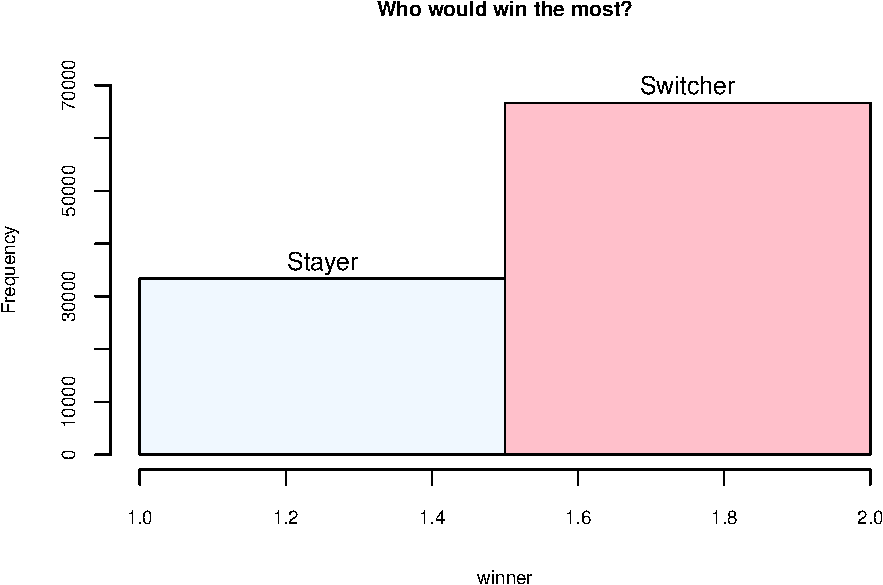
\includegraphics{07-Sim_files/figure-latex/unnamed-chunk-31-1.pdf}

The simulation is inspired by \url{https://theressomethingaboutr.wordpress.com/2019/02/12/in-memory-of-monty-hall/} \citep{Rajter_2019}

\hypertarget{exploratory-data-analysis-eda}{%
\chapter{Exploratory Data Analysis (EDA)}\label{exploratory-data-analysis-eda}}

EDA is an informal process to have an inital investigation of the data. EDA is an important part of any data analysis. For example, data cleaning is just one application of EDA: you ask questions about whether your data meets your expectations or not. To do data cleaning, you'll need to deploy all the tools of EDA: \textbf{visualisation, transformation, and modelling}.

The main steps in exploratory data analysis are:

\begin{itemize}
\tightlist
\item
  Getting the data
\item
  Dataset Overview
\item
  Visualization
\item
  Identifying missing values
\item
  Distibution of data: variations
\item
  Correlated variables
\end{itemize}

\hypertarget{getting-the-data}{%
\section{Getting the data}\label{getting-the-data}}

We will use the same data set, Ames Housing Price data from the \texttt{AmesHousing} package, containing 2930 observations and 81 features including the sale date and price.

\begin{Shaded}
\begin{Highlighting}[]
\FunctionTok{library}\NormalTok{(AmesHousing)}
\FunctionTok{library}\NormalTok{(dplyr)}
\end{Highlighting}
\end{Shaded}

\begin{verbatim}
## 
## Attaching package: 'dplyr'
\end{verbatim}

\begin{verbatim}
## The following objects are masked from 'package:stats':
## 
##     filter, lag
\end{verbatim}

\begin{verbatim}
## The following objects are masked from 'package:base':
## 
##     intersect, setdiff, setequal, union
\end{verbatim}

\begin{Shaded}
\begin{Highlighting}[]
\FunctionTok{library}\NormalTok{(DataExplorer)}
\NormalTok{amesdata }\OtherTok{\textless{}{-}} \FunctionTok{make\_ames}\NormalTok{()}
\FunctionTok{introduce}\NormalTok{(amesdata)}
\end{Highlighting}
\end{Shaded}

\begin{verbatim}
## # A tibble: 1 x 9
##    rows columns discrete_columns conti~1 all_m~2 total~3 compl~4 total~5 memor~6
##   <int>   <int>            <int>   <int>   <int>   <int>   <int>   <int>   <dbl>
## 1  2930      81               46      35       0       0    2930  237330 1146920
## # ... with abbreviated variable names 1: continuous_columns,
## #   2: all_missing_columns, 3: total_missing_values, 4: complete_rows,
## #   5: total_observations, 6: memory_usage
\end{verbatim}

\begin{Shaded}
\begin{Highlighting}[]
\FunctionTok{glimpse}\NormalTok{(amesdata)}
\end{Highlighting}
\end{Shaded}

\begin{verbatim}
## Rows: 2,930
## Columns: 81
## $ MS_SubClass        <fct> One_Story_1946_and_Newer_All_Styles, One_Story_1946~
## $ MS_Zoning          <fct> Residential_Low_Density, Residential_High_Density, ~
## $ Lot_Frontage       <dbl> 141, 80, 81, 93, 74, 78, 41, 43, 39, 60, 75, 0, 63,~
## $ Lot_Area           <int> 31770, 11622, 14267, 11160, 13830, 9978, 4920, 5005~
## $ Street             <fct> Pave, Pave, Pave, Pave, Pave, Pave, Pave, Pave, Pav~
## $ Alley              <fct> No_Alley_Access, No_Alley_Access, No_Alley_Access, ~
## $ Lot_Shape          <fct> Slightly_Irregular, Regular, Slightly_Irregular, Re~
## $ Land_Contour       <fct> Lvl, Lvl, Lvl, Lvl, Lvl, Lvl, Lvl, HLS, Lvl, Lvl, L~
## $ Utilities          <fct> AllPub, AllPub, AllPub, AllPub, AllPub, AllPub, All~
## $ Lot_Config         <fct> Corner, Inside, Corner, Corner, Inside, Inside, Ins~
## $ Land_Slope         <fct> Gtl, Gtl, Gtl, Gtl, Gtl, Gtl, Gtl, Gtl, Gtl, Gtl, G~
## $ Neighborhood       <fct> North_Ames, North_Ames, North_Ames, North_Ames, Gil~
## $ Condition_1        <fct> Norm, Feedr, Norm, Norm, Norm, Norm, Norm, Norm, No~
## $ Condition_2        <fct> Norm, Norm, Norm, Norm, Norm, Norm, Norm, Norm, Nor~
## $ Bldg_Type          <fct> OneFam, OneFam, OneFam, OneFam, OneFam, OneFam, Twn~
## $ House_Style        <fct> One_Story, One_Story, One_Story, One_Story, Two_Sto~
## $ Overall_Qual       <fct> Above_Average, Average, Above_Average, Good, Averag~
## $ Overall_Cond       <fct> Average, Above_Average, Above_Average, Average, Ave~
## $ Year_Built         <int> 1960, 1961, 1958, 1968, 1997, 1998, 2001, 1992, 199~
## $ Year_Remod_Add     <int> 1960, 1961, 1958, 1968, 1998, 1998, 2001, 1992, 199~
## $ Roof_Style         <fct> Hip, Gable, Hip, Hip, Gable, Gable, Gable, Gable, G~
## $ Roof_Matl          <fct> CompShg, CompShg, CompShg, CompShg, CompShg, CompSh~
## $ Exterior_1st       <fct> BrkFace, VinylSd, Wd Sdng, BrkFace, VinylSd, VinylS~
## $ Exterior_2nd       <fct> Plywood, VinylSd, Wd Sdng, BrkFace, VinylSd, VinylS~
## $ Mas_Vnr_Type       <fct> Stone, None, BrkFace, None, None, BrkFace, None, No~
## $ Mas_Vnr_Area       <dbl> 112, 0, 108, 0, 0, 20, 0, 0, 0, 0, 0, 0, 0, 0, 0, 6~
## $ Exter_Qual         <fct> Typical, Typical, Typical, Good, Typical, Typical, ~
## $ Exter_Cond         <fct> Typical, Typical, Typical, Typical, Typical, Typica~
## $ Foundation         <fct> CBlock, CBlock, CBlock, CBlock, PConc, PConc, PConc~
## $ Bsmt_Qual          <fct> Typical, Typical, Typical, Typical, Good, Typical, ~
## $ Bsmt_Cond          <fct> Good, Typical, Typical, Typical, Typical, Typical, ~
## $ Bsmt_Exposure      <fct> Gd, No, No, No, No, No, Mn, No, No, No, No, No, No,~
## $ BsmtFin_Type_1     <fct> BLQ, Rec, ALQ, ALQ, GLQ, GLQ, GLQ, ALQ, GLQ, Unf, U~
## $ BsmtFin_SF_1       <dbl> 2, 6, 1, 1, 3, 3, 3, 1, 3, 7, 7, 1, 7, 3, 3, 1, 3, ~
## $ BsmtFin_Type_2     <fct> Unf, LwQ, Unf, Unf, Unf, Unf, Unf, Unf, Unf, Unf, U~
## $ BsmtFin_SF_2       <dbl> 0, 144, 0, 0, 0, 0, 0, 0, 0, 0, 0, 0, 0, 0, 1120, 0~
## $ Bsmt_Unf_SF        <dbl> 441, 270, 406, 1045, 137, 324, 722, 1017, 415, 994,~
## $ Total_Bsmt_SF      <dbl> 1080, 882, 1329, 2110, 928, 926, 1338, 1280, 1595, ~
## $ Heating            <fct> GasA, GasA, GasA, GasA, GasA, GasA, GasA, GasA, Gas~
## $ Heating_QC         <fct> Fair, Typical, Typical, Excellent, Good, Excellent,~
## $ Central_Air        <fct> Y, Y, Y, Y, Y, Y, Y, Y, Y, Y, Y, Y, Y, Y, Y, Y, Y, ~
## $ Electrical         <fct> SBrkr, SBrkr, SBrkr, SBrkr, SBrkr, SBrkr, SBrkr, SB~
## $ First_Flr_SF       <int> 1656, 896, 1329, 2110, 928, 926, 1338, 1280, 1616, ~
## $ Second_Flr_SF      <int> 0, 0, 0, 0, 701, 678, 0, 0, 0, 776, 892, 0, 676, 0,~
## $ Low_Qual_Fin_SF    <int> 0, 0, 0, 0, 0, 0, 0, 0, 0, 0, 0, 0, 0, 0, 0, 0, 0, ~
## $ Gr_Liv_Area        <int> 1656, 896, 1329, 2110, 1629, 1604, 1338, 1280, 1616~
## $ Bsmt_Full_Bath     <dbl> 1, 0, 0, 1, 0, 0, 1, 0, 1, 0, 0, 1, 0, 1, 1, 1, 0, ~
## $ Bsmt_Half_Bath     <dbl> 0, 0, 0, 0, 0, 0, 0, 0, 0, 0, 0, 0, 0, 0, 0, 0, 0, ~
## $ Full_Bath          <int> 1, 1, 1, 2, 2, 2, 2, 2, 2, 2, 2, 2, 2, 1, 1, 3, 2, ~
## $ Half_Bath          <int> 0, 0, 1, 1, 1, 1, 0, 0, 0, 1, 1, 0, 1, 1, 1, 1, 0, ~
## $ Bedroom_AbvGr      <int> 3, 2, 3, 3, 3, 3, 2, 2, 2, 3, 3, 3, 3, 2, 1, 4, 4, ~
## $ Kitchen_AbvGr      <int> 1, 1, 1, 1, 1, 1, 1, 1, 1, 1, 1, 1, 1, 1, 1, 1, 1, ~
## $ Kitchen_Qual       <fct> Typical, Typical, Good, Excellent, Typical, Good, G~
## $ TotRms_AbvGrd      <int> 7, 5, 6, 8, 6, 7, 6, 5, 5, 7, 7, 6, 7, 5, 4, 12, 8,~
## $ Functional         <fct> Typ, Typ, Typ, Typ, Typ, Typ, Typ, Typ, Typ, Typ, T~
## $ Fireplaces         <int> 2, 0, 0, 2, 1, 1, 0, 0, 1, 1, 1, 0, 1, 1, 0, 1, 0, ~
## $ Fireplace_Qu       <fct> Good, No_Fireplace, No_Fireplace, Typical, Typical,~
## $ Garage_Type        <fct> Attchd, Attchd, Attchd, Attchd, Attchd, Attchd, Att~
## $ Garage_Finish      <fct> Fin, Unf, Unf, Fin, Fin, Fin, Fin, RFn, RFn, Fin, F~
## $ Garage_Cars        <dbl> 2, 1, 1, 2, 2, 2, 2, 2, 2, 2, 2, 2, 2, 2, 2, 3, 2, ~
## $ Garage_Area        <dbl> 528, 730, 312, 522, 482, 470, 582, 506, 608, 442, 4~
## $ Garage_Qual        <fct> Typical, Typical, Typical, Typical, Typical, Typica~
## $ Garage_Cond        <fct> Typical, Typical, Typical, Typical, Typical, Typica~
## $ Paved_Drive        <fct> Partial_Pavement, Paved, Paved, Paved, Paved, Paved~
## $ Wood_Deck_SF       <int> 210, 140, 393, 0, 212, 360, 0, 0, 237, 140, 157, 48~
## $ Open_Porch_SF      <int> 62, 0, 36, 0, 34, 36, 0, 82, 152, 60, 84, 21, 75, 0~
## $ Enclosed_Porch     <int> 0, 0, 0, 0, 0, 0, 170, 0, 0, 0, 0, 0, 0, 0, 0, 0, 0~
## $ Three_season_porch <int> 0, 0, 0, 0, 0, 0, 0, 0, 0, 0, 0, 0, 0, 0, 0, 0, 0, ~
## $ Screen_Porch       <int> 0, 120, 0, 0, 0, 0, 0, 144, 0, 0, 0, 0, 0, 0, 140, ~
## $ Pool_Area          <int> 0, 0, 0, 0, 0, 0, 0, 0, 0, 0, 0, 0, 0, 0, 0, 0, 0, ~
## $ Pool_QC            <fct> No_Pool, No_Pool, No_Pool, No_Pool, No_Pool, No_Poo~
## $ Fence              <fct> No_Fence, Minimum_Privacy, No_Fence, No_Fence, Mini~
## $ Misc_Feature       <fct> None, None, Gar2, None, None, None, None, None, Non~
## $ Misc_Val           <int> 0, 0, 12500, 0, 0, 0, 0, 0, 0, 0, 0, 500, 0, 0, 0, ~
## $ Mo_Sold            <int> 5, 6, 6, 4, 3, 6, 4, 1, 3, 6, 4, 3, 5, 2, 6, 6, 6, ~
## $ Year_Sold          <int> 2010, 2010, 2010, 2010, 2010, 2010, 2010, 2010, 201~
## $ Sale_Type          <fct> WD , WD , WD , WD , WD , WD , WD , WD , WD , WD , W~
## $ Sale_Condition     <fct> Normal, Normal, Normal, Normal, Normal, Normal, Nor~
## $ Sale_Price         <int> 215000, 105000, 172000, 244000, 189900, 195500, 213~
## $ Longitude          <dbl> -93.61975, -93.61976, -93.61939, -93.61732, -93.638~
## $ Latitude           <dbl> 42.05403, 42.05301, 42.05266, 42.05125, 42.06090, 4~
\end{verbatim}

\hypertarget{visualization}{%
\section{Visualization}\label{visualization}}

\hypertarget{looking-into}{%
\subsection{Looking into}\label{looking-into}}

\begin{Shaded}
\begin{Highlighting}[]
\NormalTok{amesdata }\SpecialCharTok{\%\textgreater{}\%} \FunctionTok{plot\_intro}\NormalTok{()}
\end{Highlighting}
\end{Shaded}

\includegraphics{08-EDA_files/figure-latex/unnamed-chunk-3-1.pdf}

\begin{Shaded}
\begin{Highlighting}[]
\NormalTok{amesdata }\SpecialCharTok{\%\textgreater{}\%} \FunctionTok{plot\_missing}\NormalTok{()}
\end{Highlighting}
\end{Shaded}

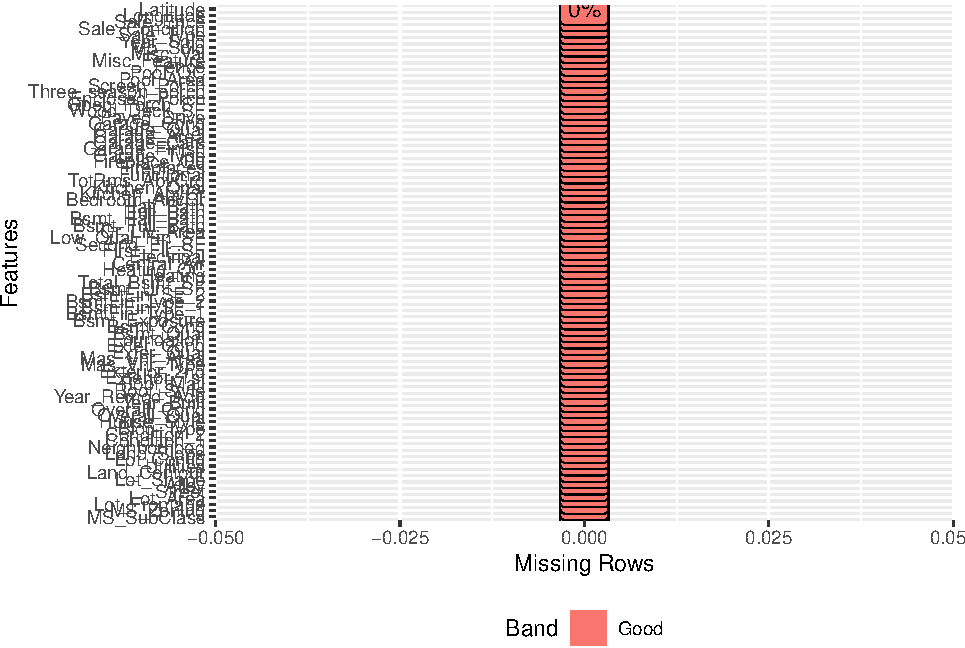
\includegraphics{08-EDA_files/figure-latex/unnamed-chunk-3-2.pdf}
Yes, our data is ``clean'' but how about this:

\begin{Shaded}
\begin{Highlighting}[]
\FunctionTok{library}\NormalTok{(forcats)}
\NormalTok{gss\_cat }\SpecialCharTok{\%\textgreater{}\%} \FunctionTok{glimpse}\NormalTok{()}
\end{Highlighting}
\end{Shaded}

\begin{verbatim}
## Rows: 21,483
## Columns: 9
## $ year    <int> 2000, 2000, 2000, 2000, 2000, 2000, 2000, 2000, 2000, 2000, 20~
## $ marital <fct> Never married, Divorced, Widowed, Never married, Divorced, Mar~
## $ age     <int> 26, 48, 67, 39, 25, 25, 36, 44, 44, 47, 53, 52, 52, 51, 52, 40~
## $ race    <fct> White, White, White, White, White, White, White, White, White,~
## $ rincome <fct> $8000 to 9999, $8000 to 9999, Not applicable, Not applicable, ~
## $ partyid <fct> "Ind,near rep", "Not str republican", "Independent", "Ind,near~
## $ relig   <fct> Protestant, Protestant, Protestant, Orthodox-christian, None, ~
## $ denom   <fct> "Southern baptist", "Baptist-dk which", "No denomination", "No~
## $ tvhours <int> 12, NA, 2, 4, 1, NA, 3, NA, 0, 3, 2, NA, 1, NA, 1, 7, NA, 3, 3~
\end{verbatim}

\begin{Shaded}
\begin{Highlighting}[]
\NormalTok{gss\_cat }\SpecialCharTok{\%\textgreater{}\%} \FunctionTok{plot\_missing}\NormalTok{()}
\end{Highlighting}
\end{Shaded}

\includegraphics{08-EDA_files/figure-latex/unnamed-chunk-4-1.pdf}

\begin{Shaded}
\begin{Highlighting}[]
\NormalTok{gss\_cat }\SpecialCharTok{\%\textgreater{}\%} \FunctionTok{profile\_missing}\NormalTok{()}
\end{Highlighting}
\end{Shaded}

\begin{verbatim}
## # A tibble: 9 x 3
##   feature num_missing pct_missing
##   <fct>         <int>       <dbl>
## 1 year              0     0      
## 2 marital           0     0      
## 3 age              76     0.00354
## 4 race              0     0      
## 5 rincome           0     0      
## 6 partyid           0     0      
## 7 relig             0     0      
## 8 denom             0     0      
## 9 tvhours       10146     0.472
\end{verbatim}

See the data source here: \url{https://forcats.tidyverse.org/reference/gss_cat.html}

\hypertarget{plots}{%
\subsection{Plots}\label{plots}}

\begin{Shaded}
\begin{Highlighting}[]
\NormalTok{amesdata  }\SpecialCharTok{\%\textgreater{}\%} \FunctionTok{plot\_density}\NormalTok{()}
\end{Highlighting}
\end{Shaded}

\includegraphics{08-EDA_files/figure-latex/unnamed-chunk-5-1.pdf} \includegraphics{08-EDA_files/figure-latex/unnamed-chunk-5-2.pdf} \includegraphics{08-EDA_files/figure-latex/unnamed-chunk-5-3.pdf}

\begin{Shaded}
\begin{Highlighting}[]
\NormalTok{gss\_cat  }\SpecialCharTok{\%\textgreater{}\%} \FunctionTok{plot\_correlation}\NormalTok{()}
\end{Highlighting}
\end{Shaded}

\begin{verbatim}
## 1 features with more than 20 categories ignored!
## denom: 30 categories
\end{verbatim}

\includegraphics{08-EDA_files/figure-latex/unnamed-chunk-6-1.pdf}
\#\# Variation \& Correlation

The ``near-zero-variance'' predictors may need to be identified and eliminated prior to modeling. We use the package \texttt{caret} to identify \href{https://topepo.github.io/caret/pre-processing.html}{``near-zero-variance'' variables}:

\begin{quote}
To identify these types of predictors, the following two metrics can be calculated:
\end{quote}

\begin{quote}
the frequency of the most prevalent value over the second most frequent value (called the ``frequency ratio'\,'), which would be near one for well-behaved predictors and very large for highly-unbalanced data and
the ``percent of unique values'\,' is the number of unique values divided by the total number of samples (times 100) that approaches zero as the granularity of the data increases
\end{quote}

\begin{quote}
If the frequency ratio is greater than a pre-specified threshold and the unique value percentage is less than a threshold, we might consider a predictor to be near zero-variance.
\end{quote}

\begin{Shaded}
\begin{Highlighting}[]
\NormalTok{caret}\SpecialCharTok{::}\FunctionTok{nearZeroVar}\NormalTok{(amesdata, }\AttributeTok{saveMetrics=} \ConstantTok{TRUE}\NormalTok{)}
\end{Highlighting}
\end{Shaded}

\begin{verbatim}
##                      freqRatio percentUnique zeroVar   nzv
## MS_SubClass           1.876522    0.54607509   FALSE FALSE
## MS_Zoning             4.919913    0.23890785   FALSE FALSE
## Lot_Frontage          1.775362    4.40273038   FALSE FALSE
## Lot_Area              1.023256   66.89419795   FALSE FALSE
## Street              243.166667    0.06825939   FALSE  TRUE
## Alley                22.766667    0.10238908   FALSE  TRUE
## Lot_Shape             1.898876    0.13651877   FALSE FALSE
## Land_Contour         21.941667    0.13651877   FALSE  TRUE
## Utilities          1463.500000    0.10238908   FALSE  TRUE
## Lot_Config            4.187867    0.17064846   FALSE FALSE
## Land_Slope           22.312000    0.10238908   FALSE  TRUE
## Neighborhood          1.659176    0.95563140   FALSE FALSE
## Condition_1          15.378049    0.30716724   FALSE FALSE
## Condition_2         223.076923    0.27303754   FALSE  TRUE
## Bldg_Type            10.407725    0.17064846   FALSE FALSE
## House_Style           1.696449    0.27303754   FALSE FALSE
## Overall_Qual          1.127049    0.34129693   FALSE FALSE
## Overall_Cond          3.103189    0.30716724   FALSE FALSE
## Year_Built            1.028986    4.02730375   FALSE FALSE
## Year_Remod_Add        1.787129    2.08191126   FALSE FALSE
## Roof_Style            4.212341    0.20477816   FALSE FALSE
## Roof_Matl           125.521739    0.27303754   FALSE  TRUE
## Exterior_1st          2.280000    0.54607509   FALSE FALSE
## Exterior_2nd          2.270694    0.58020478   FALSE FALSE
## Mas_Vnr_Type          2.017045    0.17064846   FALSE FALSE
## Mas_Vnr_Area        118.066667   15.18771331   FALSE FALSE
## Exter_Qual            1.819009    0.13651877   FALSE FALSE
## Exter_Cond            8.525084    0.17064846   FALSE FALSE
## Foundation            1.053055    0.20477816   FALSE FALSE
## Bsmt_Qual             1.052502    0.20477816   FALSE FALSE
## Bsmt_Cond            21.442623    0.20477816   FALSE  TRUE
## Bsmt_Exposure         4.559809    0.17064846   FALSE FALSE
## BsmtFin_Type_1        1.009401    0.23890785   FALSE FALSE
## BsmtFin_SF_1          1.009401    0.27303754   FALSE FALSE
## BsmtFin_Type_2       23.575472    0.23890785   FALSE  TRUE
## BsmtFin_SF_2        515.800000    9.35153584   FALSE  TRUE
## Bsmt_Unf_SF          12.894737   38.80546075   FALSE FALSE
## Total_Bsmt_SF         1.081081   36.10921502   FALSE FALSE
## Heating             106.851852    0.20477816   FALSE  TRUE
## Heating_QC            1.730324    0.17064846   FALSE FALSE
## Central_Air          13.948980    0.06825939   FALSE FALSE
## Electrical           14.265957    0.20477816   FALSE FALSE
## First_Flr_SF          1.642857   36.96245734   FALSE FALSE
## Second_Flr_SF        72.956522   21.67235495   FALSE FALSE
## Low_Qual_Fin_SF     722.500000    1.22866894   FALSE  TRUE
## Gr_Liv_Area           1.576923   44.09556314   FALSE FALSE
## Bsmt_Full_Bath        1.447079    0.13651877   FALSE FALSE
## Bsmt_Half_Bath       16.111111    0.10238908   FALSE FALSE
## Full_Bath             1.162367    0.17064846   FALSE FALSE
## Half_Bath             1.735405    0.10238908   FALSE FALSE
## Bedroom_AbvGr         2.149394    0.27303754   FALSE FALSE
## Kitchen_AbvGr        21.674419    0.13651877   FALSE  TRUE
## Kitchen_Qual          1.287931    0.17064846   FALSE FALSE
## TotRms_AbvGrd         1.300462    0.47781570   FALSE FALSE
## Functional           38.971429    0.27303754   FALSE  TRUE
## Fireplaces            1.116170    0.17064846   FALSE FALSE
## Fireplace_Qu          1.911290    0.20477816   FALSE FALSE
## Garage_Type           2.213555    0.23890785   FALSE FALSE
## Garage_Finish         1.516010    0.13651877   FALSE FALSE
## Garage_Cars           2.060411    0.20477816   FALSE FALSE
## Garage_Area           1.628866   20.58020478   FALSE FALSE
## Garage_Qual          16.446541    0.20477816   FALSE FALSE
## Garage_Cond          16.761006    0.20477816   FALSE FALSE
## Paved_Drive          12.277778    0.10238908   FALSE FALSE
## Wood_Deck_SF         20.621622   12.96928328   FALSE FALSE
## Open_Porch_SF        25.000000    8.60068259   FALSE  TRUE
## Enclosed_Porch      112.318182    6.24573379   FALSE  TRUE
## Three_season_porch  964.333333    1.05802048   FALSE  TRUE
## Screen_Porch        205.692308    4.12969283   FALSE  TRUE
## Pool_Area          2917.000000    0.47781570   FALSE  TRUE
## Pool_QC             729.250000    0.17064846   FALSE  TRUE
## Fence                 7.145455    0.17064846   FALSE FALSE
## Misc_Feature         29.726316    0.20477816   FALSE  TRUE
## Misc_Val            157.055556    1.29692833   FALSE  TRUE
## Mo_Sold               1.124722    0.40955631   FALSE FALSE
## Year_Sold             1.070988    0.17064846   FALSE FALSE
## Sale_Type            10.610879    0.34129693   FALSE FALSE
## Sale_Condition        9.848980    0.20477816   FALSE FALSE
## Sale_Price            1.030303   35.22184300   FALSE FALSE
## Longitude             1.000000   74.12969283   FALSE FALSE
## Latitude              1.111111   67.57679181   FALSE FALSE
\end{verbatim}

Again, using the package \texttt{caret}:

\begin{quote}
While there are some models that thrive on correlated predictors (such as pls), other models may benefit from reducing the level of correlation between the predictors.
\end{quote}

\begin{quote}
Given a correlation matrix, the \texttt{findCorrelation} function uses the following algorithm to flag predictors for removal:
\end{quote}

\begin{Shaded}
\begin{Highlighting}[]
\CommentTok{\#descrCor \textless{}{-}  cor(gss\_cat)}
\CommentTok{\#highCorr \textless{}{-} sum(abs(descrCor[upper.tri(descrCor)]) \textgreater{} .999)}
\end{Highlighting}
\end{Shaded}

\hypertarget{rmarkdown}{%
\section{RMarkdown}\label{rmarkdown}}

R Markdown provides an excellent platform for authoring your data science projects (like EDA's) combining your codes, their results, and your commentary. R Markdown documents support multiple output formats: HTML, PDFs, Word files, slideshows, and more.

Here are some examples

\begin{itemize}
\tightlist
\item
  html output: \url{https://raw.githack.com/yaydede/Blog_posts/main/EDA.html}
\item
  pdf output: \url{https://yaydede.github.io/files/CV6.pdf}
\end{itemize}

You can use R Markdown in many ways but here are the few main ways:

\begin{itemize}
\tightlist
\item
  For communicating to decision makers who want to focus on the conclusions, not the code behind the analysis.
\item
  For collaborating with those, who are interested in both your conclusions and the codes.
\item
  As a nice notebook where you can capture not only what you did, but also what you were thinking.
\item
  As a scientific manuscript using Latex: \url{https://www.marianamontes.me/post/academic-writing-in-r-markdown-i/}
\item
  A book with \href{https://bookdown.org}{Bookdown}: \url{https://yaydede.github.io/ToolShed/}
\item
  As a blog with \href{https://bookdown.org/yihui/blogdown/}{Blogdown}: \url{https://shilaan.rbind.io/post/building-your-website-using-r-blogdown/}
\item
  As a good \texttt{html} support for your website: \url{https://yaydede.github.io}
\end{itemize}

Our package \texttt{RBootcamp} has a template: \texttt{Worksheet1}. Locate it at \texttt{File\ \textgreater{}\ New\ File\ \textgreater{}\ R\ Markdown\ \textgreater{}\ Template}. It will give a a good starting point

\hypertarget{lessons-answers}{%
\chapter{Lessons \& Answers}\label{lessons-answers}}

There are 6 interactive lessons with a wide range of exercises. Please access them by

\begin{Shaded}
\begin{Highlighting}[]
\CommentTok{\#install.packages("remotes")}
\CommentTok{\#remotes::install\_github("yaydede/RBootcamp")}
\end{Highlighting}
\end{Shaded}

Run the following lines on your console \ldots{}

\hypertarget{lessons}{%
\section{Lessons}\label{lessons}}

\texttt{learnr::run\_tutorial("Lesson1",\ "RBootcamp")} for Ch's 1 and 2\\
\texttt{learnr::run\_tutorial("Lesson2",\ "RBootcamp")} for Ch. 4\\
\texttt{learnr::run\_tutorial("Lesson3",\ "RBootcamp")} for Ch. 5\\
\texttt{learnr::run\_tutorial("Lesson4",\ "RBootcamp")} for Ch. 6\\
\texttt{learnr::run\_tutorial("Lesson5",\ "RBootcamp")} for Ch. 7\\
\texttt{learnr::run\_tutorial("Lesson6",\ "RBootcamp")} for Ch. 8

\hypertarget{answers}{%
\section{Answers}\label{answers}}

\texttt{learnr::run\_tutorial("Lesson1A",\ "RBootcamp")}\strut \\
\texttt{learnr::run\_tutorial("Lesson2A",\ "RBootcamp")}\strut \\
\texttt{learnr::run\_tutorial("Lesson3A",\ "RBootcamp")}\strut \\
\texttt{learnr::run\_tutorial("Lesson4A",\ "RBootcamp")}\strut \\
\texttt{learnr::run\_tutorial("Lesson5A",\ "RBootcamp")}\strut \\
\texttt{learnr::run\_tutorial("Lesson6A",\ "RBootcamp")}

  \bibliography{book.bib,packages.bib}

\end{document}
